\documentclass[twoside]{book}

% Packages required by doxygen
\usepackage{fixltx2e}
\usepackage{calc}
\usepackage{doxygen}
\usepackage[export]{adjustbox} % also loads graphicx
\usepackage{graphicx}
\usepackage[utf8]{inputenc}
\usepackage{makeidx}
\usepackage{multicol}
\usepackage{multirow}
\PassOptionsToPackage{warn}{textcomp}
\usepackage{textcomp}
\usepackage[nointegrals]{wasysym}
\usepackage[table]{xcolor}

% Font selection
\usepackage[T1]{fontenc}
\usepackage[scaled=.90]{helvet}
\usepackage{courier}
\usepackage{amssymb}
\usepackage{sectsty}
\renewcommand{\familydefault}{\sfdefault}
\allsectionsfont{%
  \fontseries{bc}\selectfont%
  \color{darkgray}%
}
\renewcommand{\DoxyLabelFont}{%
  \fontseries{bc}\selectfont%
  \color{darkgray}%
}
\newcommand{\+}{\discretionary{\mbox{\scriptsize$\hookleftarrow$}}{}{}}

% Page & text layout
\usepackage{geometry}
\geometry{%
  a4paper,%
  top=2.5cm,%
  bottom=2.5cm,%
  left=2.5cm,%
  right=2.5cm%
}
\tolerance=750
\hfuzz=15pt
\hbadness=750
\setlength{\emergencystretch}{15pt}
\setlength{\parindent}{0cm}
\setlength{\parskip}{3ex plus 2ex minus 2ex}
\makeatletter
\renewcommand{\paragraph}{%
  \@startsection{paragraph}{4}{0ex}{-1.0ex}{1.0ex}{%
    \normalfont\normalsize\bfseries\SS@parafont%
  }%
}
\renewcommand{\subparagraph}{%
  \@startsection{subparagraph}{5}{0ex}{-1.0ex}{1.0ex}{%
    \normalfont\normalsize\bfseries\SS@subparafont%
  }%
}
\makeatother

% Headers & footers
\usepackage{fancyhdr}
\pagestyle{fancyplain}
\fancyhead[LE]{\fancyplain{}{\bfseries\thepage}}
\fancyhead[CE]{\fancyplain{}{}}
\fancyhead[RE]{\fancyplain{}{\bfseries\leftmark}}
\fancyhead[LO]{\fancyplain{}{\bfseries\rightmark}}
\fancyhead[CO]{\fancyplain{}{}}
\fancyhead[RO]{\fancyplain{}{\bfseries\thepage}}
\fancyfoot[LE]{\fancyplain{}{}}
\fancyfoot[CE]{\fancyplain{}{}}
\fancyfoot[RE]{\fancyplain{}{\bfseries\scriptsize Generated by Doxygen }}
\fancyfoot[LO]{\fancyplain{}{\bfseries\scriptsize Generated by Doxygen }}
\fancyfoot[CO]{\fancyplain{}{}}
\fancyfoot[RO]{\fancyplain{}{}}
\renewcommand{\footrulewidth}{0.4pt}
\renewcommand{\chaptermark}[1]{%
  \markboth{#1}{}%
}
\renewcommand{\sectionmark}[1]{%
  \markright{\thesection\ #1}%
}

% Indices & bibliography
\usepackage{natbib}
\usepackage[titles]{tocloft}
\setcounter{tocdepth}{3}
\setcounter{secnumdepth}{5}
\makeindex

% Hyperlinks (required, but should be loaded last)
\usepackage{ifpdf}
\ifpdf
  \usepackage[pdftex,pagebackref=true]{hyperref}
\else
  \usepackage[ps2pdf,pagebackref=true]{hyperref}
\fi
\hypersetup{%
  colorlinks=true,%
  linkcolor=blue,%
  citecolor=blue,%
  unicode%
}

% Custom commands
\newcommand{\clearemptydoublepage}{%
  \newpage{\pagestyle{empty}\cleardoublepage}%
}

\usepackage{caption}
\captionsetup{labelsep=space,justification=centering,font={bf},singlelinecheck=off,skip=4pt,position=top}

%===== C O N T E N T S =====

\begin{document}

% Titlepage & ToC
\hypersetup{pageanchor=false,
             bookmarksnumbered=true,
             pdfencoding=unicode
            }
\pagenumbering{roman}
\begin{titlepage}
\vspace*{7cm}
\begin{center}%
{\Large Daimtronics }\\
\vspace*{1cm}
{\large Generated by Doxygen 1.8.11}\\
\end{center}
\end{titlepage}
\clearemptydoublepage
\tableofcontents
\clearemptydoublepage
\pagenumbering{arabic}
\hypersetup{pageanchor=true}

%--- Begin generated contents ---
\chapter{Namespace Index}
\section{Namespace List}
Here is a list of all namespaces with brief descriptions\+:\begin{DoxyCompactList}
\item\contentsline{section}{\hyperlink{namespaceros}{ros} }{\pageref{namespaceros}}{}
\item\contentsline{section}{\hyperlink{namespaceros_1_1message__operations}{ros\+::message\+\_\+operations} }{\pageref{namespaceros_1_1message__operations}}{}
\item\contentsline{section}{\hyperlink{namespaceros_1_1message__traits}{ros\+::message\+\_\+traits} }{\pageref{namespaceros_1_1message__traits}}{}
\item\contentsline{section}{\hyperlink{namespaceros_1_1serialization}{ros\+::serialization} }{\pageref{namespaceros_1_1serialization}}{}
\item\contentsline{section}{\hyperlink{namespacesemi__truck}{semi\+\_\+truck} }{\pageref{namespacesemi__truck}}{}
\end{DoxyCompactList}

\chapter{Hierarchical Index}
\section{Class Hierarchy}
This inheritance list is sorted roughly, but not completely, alphabetically\+:\begin{DoxyCompactList}
\item \contentsline{section}{actuator\+\_\+data\+\_\+t}{\pageref{structactuator__data__t}}{}
\item \contentsline{section}{ros\+:\+:message\+\_\+traits\+:\+:Data\+Type$<$ \+:\+:semi\+\_\+truck\+:\+:Teensy\+\_\+\+Actuators\+\_\+$<$ Container\+Allocator $>$ $>$}{\pageref{structros_1_1message__traits_1_1_data_type_3_01_1_1semi__truck_1_1_teensy___actuators___3_01_container_allocator_01_4_01_4}}{}
\item \contentsline{section}{ros\+:\+:message\+\_\+traits\+:\+:Data\+Type$<$ \+:\+:semi\+\_\+truck\+:\+:Teensy\+\_\+\+Sensors\+\_\+$<$ Container\+Allocator $>$ $>$}{\pageref{structros_1_1message__traits_1_1_data_type_3_01_1_1semi__truck_1_1_teensy___sensors___3_01_container_allocator_01_4_01_4}}{}
\item \contentsline{section}{ros\+:\+:message\+\_\+traits\+:\+:Definition$<$ \+:\+:semi\+\_\+truck\+:\+:Teensy\+\_\+\+Actuators\+\_\+$<$ Container\+Allocator $>$ $>$}{\pageref{structros_1_1message__traits_1_1_definition_3_01_1_1semi__truck_1_1_teensy___actuators___3_01_container_allocator_01_4_01_4}}{}
\item \contentsline{section}{ros\+:\+:message\+\_\+traits\+:\+:Definition$<$ \+:\+:semi\+\_\+truck\+:\+:Teensy\+\_\+\+Sensors\+\_\+$<$ Container\+Allocator $>$ $>$}{\pageref{structros_1_1message__traits_1_1_definition_3_01_1_1semi__truck_1_1_teensy___sensors___3_01_container_allocator_01_4_01_4}}{}
\item False\+Type\begin{DoxyCompactList}
\item \contentsline{section}{ros\+:\+:message\+\_\+traits\+:\+:Has\+Header$<$ \+:\+:semi\+\_\+truck\+:\+:Teensy\+\_\+\+Actuators\+\_\+$<$ Container\+Allocator $>$ $>$}{\pageref{structros_1_1message__traits_1_1_has_header_3_01_1_1semi__truck_1_1_teensy___actuators___3_01_container_allocator_01_4_01_4}}{}
\item \contentsline{section}{ros\+:\+:message\+\_\+traits\+:\+:Has\+Header$<$ \+:\+:semi\+\_\+truck\+:\+:Teensy\+\_\+\+Actuators\+\_\+$<$ Container\+Allocator $>$ const $>$}{\pageref{structros_1_1message__traits_1_1_has_header_3_01_1_1semi__truck_1_1_teensy___actuators___3_01_coe86513e6694fc989720644eb04b2c486}}{}
\item \contentsline{section}{ros\+:\+:message\+\_\+traits\+:\+:Has\+Header$<$ \+:\+:semi\+\_\+truck\+:\+:Teensy\+\_\+\+Sensors\+\_\+$<$ Container\+Allocator $>$ $>$}{\pageref{structros_1_1message__traits_1_1_has_header_3_01_1_1semi__truck_1_1_teensy___sensors___3_01_container_allocator_01_4_01_4}}{}
\item \contentsline{section}{ros\+:\+:message\+\_\+traits\+:\+:Has\+Header$<$ \+:\+:semi\+\_\+truck\+:\+:Teensy\+\_\+\+Sensors\+\_\+$<$ Container\+Allocator $>$ const $>$}{\pageref{structros_1_1message__traits_1_1_has_header_3_01_1_1semi__truck_1_1_teensy___sensors___3_01_cont27420888fce5a6e96344b08bcfbbf57b}}{}
\end{DoxyCompactList}
\item \contentsline{section}{ros\+:\+:message\+\_\+traits\+:\+:M\+D5\+Sum$<$ \+:\+:semi\+\_\+truck\+:\+:Teensy\+\_\+\+Actuators\+\_\+$<$ Container\+Allocator $>$ $>$}{\pageref{structros_1_1message__traits_1_1_m_d5_sum_3_01_1_1semi__truck_1_1_teensy___actuators___3_01_container_allocator_01_4_01_4}}{}
\item \contentsline{section}{ros\+:\+:message\+\_\+traits\+:\+:M\+D5\+Sum$<$ \+:\+:semi\+\_\+truck\+:\+:Teensy\+\_\+\+Sensors\+\_\+$<$ Container\+Allocator $>$ $>$}{\pageref{structros_1_1message__traits_1_1_m_d5_sum_3_01_1_1semi__truck_1_1_teensy___sensors___3_01_container_allocator_01_4_01_4}}{}
\item \contentsline{section}{ros\+:\+:message\+\_\+operations\+:\+:Printer$<$ \+:\+:semi\+\_\+truck\+:\+:Teensy\+\_\+\+Actuators\+\_\+$<$ Container\+Allocator $>$ $>$}{\pageref{structros_1_1message__operations_1_1_printer_3_01_1_1semi__truck_1_1_teensy___actuators___3_01_container_allocator_01_4_01_4}}{}
\item \contentsline{section}{ros\+:\+:message\+\_\+operations\+:\+:Printer$<$ \+:\+:semi\+\_\+truck\+:\+:Teensy\+\_\+\+Sensors\+\_\+$<$ Container\+Allocator $>$ $>$}{\pageref{structros_1_1message__operations_1_1_printer_3_01_1_1semi__truck_1_1_teensy___sensors___3_01_container_allocator_01_4_01_4}}{}
\item \contentsline{section}{sensor\+\_\+data\+\_\+t}{\pageref{structsensor__data__t}}{}
\item \contentsline{section}{ros\+:\+:serialization\+:\+:Serializer$<$ \+:\+:semi\+\_\+truck\+:\+:Teensy\+\_\+\+Actuators\+\_\+$<$ Container\+Allocator $>$ $>$}{\pageref{structros_1_1serialization_1_1_serializer_3_01_1_1semi__truck_1_1_teensy___actuators___3_01_container_allocator_01_4_01_4}}{}
\item \contentsline{section}{ros\+:\+:serialization\+:\+:Serializer$<$ \+:\+:semi\+\_\+truck\+:\+:Teensy\+\_\+\+Sensors\+\_\+$<$ Container\+Allocator $>$ $>$}{\pageref{structros_1_1serialization_1_1_serializer_3_01_1_1semi__truck_1_1_teensy___sensors___3_01_container_allocator_01_4_01_4}}{}
\item \contentsline{section}{system\+\_\+data\+\_\+t}{\pageref{structsystem__data__t}}{}
\item \contentsline{section}{semi\+\_\+truck\+:\+:Teensy\+\_\+\+Actuators\+\_\+$<$ Container\+Allocator $>$}{\pageref{structsemi__truck_1_1_teensy___actuators__}}{}
\item \contentsline{section}{semi\+\_\+truck\+:\+:Teensy\+\_\+\+Sensors\+\_\+$<$ Container\+Allocator $>$}{\pageref{structsemi__truck_1_1_teensy___sensors__}}{}
\item True\+Type\begin{DoxyCompactList}
\item \contentsline{section}{ros\+:\+:message\+\_\+traits\+:\+:Is\+Fixed\+Size$<$ \+:\+:semi\+\_\+truck\+:\+:Teensy\+\_\+\+Actuators\+\_\+$<$ Container\+Allocator $>$ $>$}{\pageref{structros_1_1message__traits_1_1_is_fixed_size_3_01_1_1semi__truck_1_1_teensy___actuators___3_01_container_allocator_01_4_01_4}}{}
\item \contentsline{section}{ros\+:\+:message\+\_\+traits\+:\+:Is\+Fixed\+Size$<$ \+:\+:semi\+\_\+truck\+:\+:Teensy\+\_\+\+Actuators\+\_\+$<$ Container\+Allocator $>$ const $>$}{\pageref{structros_1_1message__traits_1_1_is_fixed_size_3_01_1_1semi__truck_1_1_teensy___actuators___3_01e88fb587a6d6e04d6a7968cdf33bb127}}{}
\item \contentsline{section}{ros\+:\+:message\+\_\+traits\+:\+:Is\+Fixed\+Size$<$ \+:\+:semi\+\_\+truck\+:\+:Teensy\+\_\+\+Sensors\+\_\+$<$ Container\+Allocator $>$ $>$}{\pageref{structros_1_1message__traits_1_1_is_fixed_size_3_01_1_1semi__truck_1_1_teensy___sensors___3_01_container_allocator_01_4_01_4}}{}
\item \contentsline{section}{ros\+:\+:message\+\_\+traits\+:\+:Is\+Fixed\+Size$<$ \+:\+:semi\+\_\+truck\+:\+:Teensy\+\_\+\+Sensors\+\_\+$<$ Container\+Allocator $>$ const $>$}{\pageref{structros_1_1message__traits_1_1_is_fixed_size_3_01_1_1semi__truck_1_1_teensy___sensors___3_01_cb53d5848a141775744a1974dc7127755}}{}
\item \contentsline{section}{ros\+:\+:message\+\_\+traits\+:\+:Is\+Message$<$ \+:\+:semi\+\_\+truck\+:\+:Teensy\+\_\+\+Actuators\+\_\+$<$ Container\+Allocator $>$ $>$}{\pageref{structros_1_1message__traits_1_1_is_message_3_01_1_1semi__truck_1_1_teensy___actuators___3_01_container_allocator_01_4_01_4}}{}
\item \contentsline{section}{ros\+:\+:message\+\_\+traits\+:\+:Is\+Message$<$ \+:\+:semi\+\_\+truck\+:\+:Teensy\+\_\+\+Actuators\+\_\+$<$ Container\+Allocator $>$ const $>$}{\pageref{structros_1_1message__traits_1_1_is_message_3_01_1_1semi__truck_1_1_teensy___actuators___3_01_cobc29fbe598d16bac74a311be55406c9e}}{}
\item \contentsline{section}{ros\+:\+:message\+\_\+traits\+:\+:Is\+Message$<$ \+:\+:semi\+\_\+truck\+:\+:Teensy\+\_\+\+Sensors\+\_\+$<$ Container\+Allocator $>$ $>$}{\pageref{structros_1_1message__traits_1_1_is_message_3_01_1_1semi__truck_1_1_teensy___sensors___3_01_container_allocator_01_4_01_4}}{}
\item \contentsline{section}{ros\+:\+:message\+\_\+traits\+:\+:Is\+Message$<$ \+:\+:semi\+\_\+truck\+:\+:Teensy\+\_\+\+Sensors\+\_\+$<$ Container\+Allocator $>$ const $>$}{\pageref{structros_1_1message__traits_1_1_is_message_3_01_1_1semi__truck_1_1_teensy___sensors___3_01_contee20f324312af52498809118a40cc274}}{}
\end{DoxyCompactList}
\end{DoxyCompactList}

\chapter{Class Index}
\section{Class List}
Here are the classes, structs, unions and interfaces with brief descriptions\+:\begin{DoxyCompactList}
\item\contentsline{section}{\hyperlink{structactuator__data__t}{actuator\+\_\+data\+\_\+t} }{\pageref{structactuator__data__t}}{}
\item\contentsline{section}{\hyperlink{structros_1_1message__traits_1_1_data_type_3_01_1_1semi__truck_1_1_teensy___actuators___3_01_container_allocator_01_4_01_4}{ros\+::message\+\_\+traits\+::\+Data\+Type$<$ \+::semi\+\_\+truck\+::\+Teensy\+\_\+\+Actuators\+\_\+$<$ Container\+Allocator $>$ $>$} }{\pageref{structros_1_1message__traits_1_1_data_type_3_01_1_1semi__truck_1_1_teensy___actuators___3_01_container_allocator_01_4_01_4}}{}
\item\contentsline{section}{\hyperlink{structros_1_1message__traits_1_1_data_type_3_01_1_1semi__truck_1_1_teensy___sensors___3_01_container_allocator_01_4_01_4}{ros\+::message\+\_\+traits\+::\+Data\+Type$<$ \+::semi\+\_\+truck\+::\+Teensy\+\_\+\+Sensors\+\_\+$<$ Container\+Allocator $>$ $>$} }{\pageref{structros_1_1message__traits_1_1_data_type_3_01_1_1semi__truck_1_1_teensy___sensors___3_01_container_allocator_01_4_01_4}}{}
\item\contentsline{section}{\hyperlink{structros_1_1message__traits_1_1_definition_3_01_1_1semi__truck_1_1_teensy___actuators___3_01_container_allocator_01_4_01_4}{ros\+::message\+\_\+traits\+::\+Definition$<$ \+::semi\+\_\+truck\+::\+Teensy\+\_\+\+Actuators\+\_\+$<$ Container\+Allocator $>$ $>$} }{\pageref{structros_1_1message__traits_1_1_definition_3_01_1_1semi__truck_1_1_teensy___actuators___3_01_container_allocator_01_4_01_4}}{}
\item\contentsline{section}{\hyperlink{structros_1_1message__traits_1_1_definition_3_01_1_1semi__truck_1_1_teensy___sensors___3_01_container_allocator_01_4_01_4}{ros\+::message\+\_\+traits\+::\+Definition$<$ \+::semi\+\_\+truck\+::\+Teensy\+\_\+\+Sensors\+\_\+$<$ Container\+Allocator $>$ $>$} }{\pageref{structros_1_1message__traits_1_1_definition_3_01_1_1semi__truck_1_1_teensy___sensors___3_01_container_allocator_01_4_01_4}}{}
\item\contentsline{section}{\hyperlink{structros_1_1message__traits_1_1_has_header_3_01_1_1semi__truck_1_1_teensy___actuators___3_01_container_allocator_01_4_01_4}{ros\+::message\+\_\+traits\+::\+Has\+Header$<$ \+::semi\+\_\+truck\+::\+Teensy\+\_\+\+Actuators\+\_\+$<$ Container\+Allocator $>$ $>$} }{\pageref{structros_1_1message__traits_1_1_has_header_3_01_1_1semi__truck_1_1_teensy___actuators___3_01_container_allocator_01_4_01_4}}{}
\item\contentsline{section}{\hyperlink{structros_1_1message__traits_1_1_has_header_3_01_1_1semi__truck_1_1_teensy___actuators___3_01_coe86513e6694fc989720644eb04b2c486}{ros\+::message\+\_\+traits\+::\+Has\+Header$<$ \+::semi\+\_\+truck\+::\+Teensy\+\_\+\+Actuators\+\_\+$<$ Container\+Allocator $>$ const  $>$} }{\pageref{structros_1_1message__traits_1_1_has_header_3_01_1_1semi__truck_1_1_teensy___actuators___3_01_coe86513e6694fc989720644eb04b2c486}}{}
\item\contentsline{section}{\hyperlink{structros_1_1message__traits_1_1_has_header_3_01_1_1semi__truck_1_1_teensy___sensors___3_01_container_allocator_01_4_01_4}{ros\+::message\+\_\+traits\+::\+Has\+Header$<$ \+::semi\+\_\+truck\+::\+Teensy\+\_\+\+Sensors\+\_\+$<$ Container\+Allocator $>$ $>$} }{\pageref{structros_1_1message__traits_1_1_has_header_3_01_1_1semi__truck_1_1_teensy___sensors___3_01_container_allocator_01_4_01_4}}{}
\item\contentsline{section}{\hyperlink{structros_1_1message__traits_1_1_has_header_3_01_1_1semi__truck_1_1_teensy___sensors___3_01_cont27420888fce5a6e96344b08bcfbbf57b}{ros\+::message\+\_\+traits\+::\+Has\+Header$<$ \+::semi\+\_\+truck\+::\+Teensy\+\_\+\+Sensors\+\_\+$<$ Container\+Allocator $>$ const  $>$} }{\pageref{structros_1_1message__traits_1_1_has_header_3_01_1_1semi__truck_1_1_teensy___sensors___3_01_cont27420888fce5a6e96344b08bcfbbf57b}}{}
\item\contentsline{section}{\hyperlink{structros_1_1message__traits_1_1_is_fixed_size_3_01_1_1semi__truck_1_1_teensy___actuators___3_01_container_allocator_01_4_01_4}{ros\+::message\+\_\+traits\+::\+Is\+Fixed\+Size$<$ \+::semi\+\_\+truck\+::\+Teensy\+\_\+\+Actuators\+\_\+$<$ Container\+Allocator $>$ $>$} }{\pageref{structros_1_1message__traits_1_1_is_fixed_size_3_01_1_1semi__truck_1_1_teensy___actuators___3_01_container_allocator_01_4_01_4}}{}
\item\contentsline{section}{\hyperlink{structros_1_1message__traits_1_1_is_fixed_size_3_01_1_1semi__truck_1_1_teensy___actuators___3_01e88fb587a6d6e04d6a7968cdf33bb127}{ros\+::message\+\_\+traits\+::\+Is\+Fixed\+Size$<$ \+::semi\+\_\+truck\+::\+Teensy\+\_\+\+Actuators\+\_\+$<$ Container\+Allocator $>$ const  $>$} }{\pageref{structros_1_1message__traits_1_1_is_fixed_size_3_01_1_1semi__truck_1_1_teensy___actuators___3_01e88fb587a6d6e04d6a7968cdf33bb127}}{}
\item\contentsline{section}{\hyperlink{structros_1_1message__traits_1_1_is_fixed_size_3_01_1_1semi__truck_1_1_teensy___sensors___3_01_container_allocator_01_4_01_4}{ros\+::message\+\_\+traits\+::\+Is\+Fixed\+Size$<$ \+::semi\+\_\+truck\+::\+Teensy\+\_\+\+Sensors\+\_\+$<$ Container\+Allocator $>$ $>$} }{\pageref{structros_1_1message__traits_1_1_is_fixed_size_3_01_1_1semi__truck_1_1_teensy___sensors___3_01_container_allocator_01_4_01_4}}{}
\item\contentsline{section}{\hyperlink{structros_1_1message__traits_1_1_is_fixed_size_3_01_1_1semi__truck_1_1_teensy___sensors___3_01_cb53d5848a141775744a1974dc7127755}{ros\+::message\+\_\+traits\+::\+Is\+Fixed\+Size$<$ \+::semi\+\_\+truck\+::\+Teensy\+\_\+\+Sensors\+\_\+$<$ Container\+Allocator $>$ const  $>$} }{\pageref{structros_1_1message__traits_1_1_is_fixed_size_3_01_1_1semi__truck_1_1_teensy___sensors___3_01_cb53d5848a141775744a1974dc7127755}}{}
\item\contentsline{section}{\hyperlink{structros_1_1message__traits_1_1_is_message_3_01_1_1semi__truck_1_1_teensy___actuators___3_01_container_allocator_01_4_01_4}{ros\+::message\+\_\+traits\+::\+Is\+Message$<$ \+::semi\+\_\+truck\+::\+Teensy\+\_\+\+Actuators\+\_\+$<$ Container\+Allocator $>$ $>$} }{\pageref{structros_1_1message__traits_1_1_is_message_3_01_1_1semi__truck_1_1_teensy___actuators___3_01_container_allocator_01_4_01_4}}{}
\item\contentsline{section}{\hyperlink{structros_1_1message__traits_1_1_is_message_3_01_1_1semi__truck_1_1_teensy___actuators___3_01_cobc29fbe598d16bac74a311be55406c9e}{ros\+::message\+\_\+traits\+::\+Is\+Message$<$ \+::semi\+\_\+truck\+::\+Teensy\+\_\+\+Actuators\+\_\+$<$ Container\+Allocator $>$ const  $>$} }{\pageref{structros_1_1message__traits_1_1_is_message_3_01_1_1semi__truck_1_1_teensy___actuators___3_01_cobc29fbe598d16bac74a311be55406c9e}}{}
\item\contentsline{section}{\hyperlink{structros_1_1message__traits_1_1_is_message_3_01_1_1semi__truck_1_1_teensy___sensors___3_01_container_allocator_01_4_01_4}{ros\+::message\+\_\+traits\+::\+Is\+Message$<$ \+::semi\+\_\+truck\+::\+Teensy\+\_\+\+Sensors\+\_\+$<$ Container\+Allocator $>$ $>$} }{\pageref{structros_1_1message__traits_1_1_is_message_3_01_1_1semi__truck_1_1_teensy___sensors___3_01_container_allocator_01_4_01_4}}{}
\item\contentsline{section}{\hyperlink{structros_1_1message__traits_1_1_is_message_3_01_1_1semi__truck_1_1_teensy___sensors___3_01_contee20f324312af52498809118a40cc274}{ros\+::message\+\_\+traits\+::\+Is\+Message$<$ \+::semi\+\_\+truck\+::\+Teensy\+\_\+\+Sensors\+\_\+$<$ Container\+Allocator $>$ const  $>$} }{\pageref{structros_1_1message__traits_1_1_is_message_3_01_1_1semi__truck_1_1_teensy___sensors___3_01_contee20f324312af52498809118a40cc274}}{}
\item\contentsline{section}{\hyperlink{structros_1_1message__traits_1_1_m_d5_sum_3_01_1_1semi__truck_1_1_teensy___actuators___3_01_container_allocator_01_4_01_4}{ros\+::message\+\_\+traits\+::\+M\+D5\+Sum$<$ \+::semi\+\_\+truck\+::\+Teensy\+\_\+\+Actuators\+\_\+$<$ Container\+Allocator $>$ $>$} }{\pageref{structros_1_1message__traits_1_1_m_d5_sum_3_01_1_1semi__truck_1_1_teensy___actuators___3_01_container_allocator_01_4_01_4}}{}
\item\contentsline{section}{\hyperlink{structros_1_1message__traits_1_1_m_d5_sum_3_01_1_1semi__truck_1_1_teensy___sensors___3_01_container_allocator_01_4_01_4}{ros\+::message\+\_\+traits\+::\+M\+D5\+Sum$<$ \+::semi\+\_\+truck\+::\+Teensy\+\_\+\+Sensors\+\_\+$<$ Container\+Allocator $>$ $>$} }{\pageref{structros_1_1message__traits_1_1_m_d5_sum_3_01_1_1semi__truck_1_1_teensy___sensors___3_01_container_allocator_01_4_01_4}}{}
\item\contentsline{section}{\hyperlink{structros_1_1message__operations_1_1_printer_3_01_1_1semi__truck_1_1_teensy___actuators___3_01_container_allocator_01_4_01_4}{ros\+::message\+\_\+operations\+::\+Printer$<$ \+::semi\+\_\+truck\+::\+Teensy\+\_\+\+Actuators\+\_\+$<$ Container\+Allocator $>$ $>$} }{\pageref{structros_1_1message__operations_1_1_printer_3_01_1_1semi__truck_1_1_teensy___actuators___3_01_container_allocator_01_4_01_4}}{}
\item\contentsline{section}{\hyperlink{structros_1_1message__operations_1_1_printer_3_01_1_1semi__truck_1_1_teensy___sensors___3_01_container_allocator_01_4_01_4}{ros\+::message\+\_\+operations\+::\+Printer$<$ \+::semi\+\_\+truck\+::\+Teensy\+\_\+\+Sensors\+\_\+$<$ Container\+Allocator $>$ $>$} }{\pageref{structros_1_1message__operations_1_1_printer_3_01_1_1semi__truck_1_1_teensy___sensors___3_01_container_allocator_01_4_01_4}}{}
\item\contentsline{section}{\hyperlink{structsensor__data__t}{sensor\+\_\+data\+\_\+t} }{\pageref{structsensor__data__t}}{}
\item\contentsline{section}{\hyperlink{structros_1_1serialization_1_1_serializer_3_01_1_1semi__truck_1_1_teensy___actuators___3_01_container_allocator_01_4_01_4}{ros\+::serialization\+::\+Serializer$<$ \+::semi\+\_\+truck\+::\+Teensy\+\_\+\+Actuators\+\_\+$<$ Container\+Allocator $>$ $>$} }{\pageref{structros_1_1serialization_1_1_serializer_3_01_1_1semi__truck_1_1_teensy___actuators___3_01_container_allocator_01_4_01_4}}{}
\item\contentsline{section}{\hyperlink{structros_1_1serialization_1_1_serializer_3_01_1_1semi__truck_1_1_teensy___sensors___3_01_container_allocator_01_4_01_4}{ros\+::serialization\+::\+Serializer$<$ \+::semi\+\_\+truck\+::\+Teensy\+\_\+\+Sensors\+\_\+$<$ Container\+Allocator $>$ $>$} }{\pageref{structros_1_1serialization_1_1_serializer_3_01_1_1semi__truck_1_1_teensy___sensors___3_01_container_allocator_01_4_01_4}}{}
\item\contentsline{section}{\hyperlink{structsystem__data__t}{system\+\_\+data\+\_\+t} }{\pageref{structsystem__data__t}}{}
\item\contentsline{section}{\hyperlink{structsemi__truck_1_1_teensy___actuators__}{semi\+\_\+truck\+::\+Teensy\+\_\+\+Actuators\+\_\+$<$ Container\+Allocator $>$} }{\pageref{structsemi__truck_1_1_teensy___actuators__}}{}
\item\contentsline{section}{\hyperlink{structsemi__truck_1_1_teensy___sensors__}{semi\+\_\+truck\+::\+Teensy\+\_\+\+Sensors\+\_\+$<$ Container\+Allocator $>$} }{\pageref{structsemi__truck_1_1_teensy___sensors__}}{}
\end{DoxyCompactList}

\chapter{File Index}
\section{File List}
Here is a list of all files with brief descriptions\+:\begin{DoxyCompactList}
\item\contentsline{section}{daimtronics/semi\+\_\+catkin\+\_\+ws/src/semi\+\_\+truck/\hyperlink{package_8xml}{package.\+xml} }{\pageref{package_8xml}}{}
\item\contentsline{section}{daimtronics/semi\+\_\+catkin\+\_\+ws/src/semi\+\_\+truck/include/\hyperlink{semi__catkin__ws_2src_2semi__truck_2include_2system__data_8h}{system\+\_\+data.\+h} }{\pageref{semi__catkin__ws_2src_2semi__truck_2include_2system__data_8h}}{}
\item\contentsline{section}{daimtronics/semi\+\_\+catkin\+\_\+ws/src/semi\+\_\+truck/include/\hyperlink{_teensy___actuators_8h}{Teensy\+\_\+\+Actuators.\+h} }{\pageref{_teensy___actuators_8h}}{}
\item\contentsline{section}{daimtronics/semi\+\_\+catkin\+\_\+ws/src/semi\+\_\+truck/include/\hyperlink{_teensy___sensors_8h}{Teensy\+\_\+\+Sensors.\+h} }{\pageref{_teensy___sensors_8h}}{}
\item\contentsline{section}{daimtronics/semi\+\_\+catkin\+\_\+ws/src/semi\+\_\+truck/msg/\hyperlink{_teensy___actuators_8msg}{Teensy\+\_\+\+Actuators.\+msg} }{\pageref{_teensy___actuators_8msg}}{}
\item\contentsline{section}{daimtronics/semi\+\_\+catkin\+\_\+ws/src/semi\+\_\+truck/msg/\hyperlink{_teensy___sensors_8msg}{Teensy\+\_\+\+Sensors.\+msg} }{\pageref{_teensy___sensors_8msg}}{}
\item\contentsline{section}{daimtronics/semi\+\_\+catkin\+\_\+ws/src/semi\+\_\+truck/src/\hyperlink{pi__comm__node_8cpp}{pi\+\_\+comm\+\_\+node.\+cpp} }{\pageref{pi__comm__node_8cpp}}{}
\item\contentsline{section}{daimtronics/semi\+\_\+catkin\+\_\+ws/src/semi\+\_\+truck/src/\hyperlink{pi__comm__node_8h}{pi\+\_\+comm\+\_\+node.\+h} }{\pageref{pi__comm__node_8h}}{}
\item\contentsline{section}{daimtronics/semi\+\_\+catkin\+\_\+ws/src/semi\+\_\+truck/src/\hyperlink{semi__truck__api_8cpp}{semi\+\_\+truck\+\_\+api.\+cpp} }{\pageref{semi__truck__api_8cpp}}{}
\item\contentsline{section}{daimtronics/semi\+\_\+catkin\+\_\+ws/src/semi\+\_\+truck/src/\hyperlink{semi__truck__api_8h}{semi\+\_\+truck\+\_\+api.\+h} }{\pageref{semi__truck__api_8h}}{}
\item\contentsline{section}{daimtronics/semi\+\_\+catkin\+\_\+ws/src/semi\+\_\+truck/src/\hyperlink{truck__template__node_8cpp}{truck\+\_\+template\+\_\+node.\+cpp} }{\pageref{truck__template__node_8cpp}}{}
\item\contentsline{section}{daimtronics/teensy\+\_\+chibios/src/\hyperlink{_8_d_s___store}{.\+D\+S\+\_\+\+Store} }{\pageref{_8_d_s___store}}{}
\item\contentsline{section}{daimtronics/teensy\+\_\+chibios/src/main/\hyperlink{fifth__wheel_8cpp}{fifth\+\_\+wheel.\+cpp} }{\pageref{fifth__wheel_8cpp}}{}
\item\contentsline{section}{daimtronics/teensy\+\_\+chibios/src/main/\hyperlink{hall__sensor_8cpp}{hall\+\_\+sensor.\+cpp} }{\pageref{hall__sensor_8cpp}}{}
\item\contentsline{section}{daimtronics/teensy\+\_\+chibios/src/main/\hyperlink{imu_8cpp}{imu.\+cpp} }{\pageref{imu_8cpp}}{}
\item\contentsline{section}{daimtronics/teensy\+\_\+chibios/src/main/\hyperlink{main_8ino}{main.\+ino} }{\pageref{main_8ino}}{}
\item\contentsline{section}{daimtronics/teensy\+\_\+chibios/src/main/\hyperlink{motor__driver_8cpp}{motor\+\_\+driver.\+cpp} }{\pageref{motor__driver_8cpp}}{}
\item\contentsline{section}{daimtronics/teensy\+\_\+chibios/src/main/\hyperlink{range__finder_8cpp}{range\+\_\+finder.\+cpp} }{\pageref{range__finder_8cpp}}{}
\item\contentsline{section}{daimtronics/teensy\+\_\+chibios/src/main/\hyperlink{_r_c__receiver_8cpp}{R\+C\+\_\+receiver.\+cpp} }{\pageref{_r_c__receiver_8cpp}}{}
\item\contentsline{section}{daimtronics/teensy\+\_\+chibios/src/main/\hyperlink{steer__servo_8cpp}{steer\+\_\+servo.\+cpp} }{\pageref{steer__servo_8cpp}}{}
\item\contentsline{section}{daimtronics/teensy\+\_\+chibios/src/main/\hyperlink{tca__selector_8cpp}{tca\+\_\+selector.\+cpp} }{\pageref{tca__selector_8cpp}}{}
\item\contentsline{section}{daimtronics/teensy\+\_\+chibios/src/main/\hyperlink{teensy__serial_8cpp}{teensy\+\_\+serial.\+cpp} }{\pageref{teensy__serial_8cpp}}{}
\item\contentsline{section}{daimtronics/teensy\+\_\+chibios/src/main/\hyperlink{tof__lidar_8cpp}{tof\+\_\+lidar.\+cpp} }{\pageref{tof__lidar_8cpp}}{}
\item\contentsline{section}{daimtronics/teensy\+\_\+chibios/src/main/\hyperlink{wheel__speed_8cpp}{wheel\+\_\+speed.\+cpp} }{\pageref{wheel__speed_8cpp}}{}
\item\contentsline{section}{daimtronics/teensy\+\_\+chibios/src/main/include/\hyperlink{fifth__wheel_8h}{fifth\+\_\+wheel.\+h} }{\pageref{fifth__wheel_8h}}{}
\item\contentsline{section}{daimtronics/teensy\+\_\+chibios/src/main/include/\hyperlink{hall__sensor_8h}{hall\+\_\+sensor.\+h} }{\pageref{hall__sensor_8h}}{}
\item\contentsline{section}{daimtronics/teensy\+\_\+chibios/src/main/include/\hyperlink{imu_8h}{imu.\+h} }{\pageref{imu_8h}}{}
\item\contentsline{section}{daimtronics/teensy\+\_\+chibios/src/main/include/\hyperlink{motor__driver_8h}{motor\+\_\+driver.\+h} }{\pageref{motor__driver_8h}}{}
\item\contentsline{section}{daimtronics/teensy\+\_\+chibios/src/main/include/\hyperlink{range__finder_8h}{range\+\_\+finder.\+h} }{\pageref{range__finder_8h}}{}
\item\contentsline{section}{daimtronics/teensy\+\_\+chibios/src/main/include/\hyperlink{_r_c__receiver_8h}{R\+C\+\_\+receiver.\+h} }{\pageref{_r_c__receiver_8h}}{}
\item\contentsline{section}{daimtronics/teensy\+\_\+chibios/src/main/include/\hyperlink{steer__servo_8h}{steer\+\_\+servo.\+h} }{\pageref{steer__servo_8h}}{}
\item\contentsline{section}{daimtronics/teensy\+\_\+chibios/src/main/include/\hyperlink{teensy__chibios_2src_2main_2include_2system__data_8h}{system\+\_\+data.\+h} }{\pageref{teensy__chibios_2src_2main_2include_2system__data_8h}}{}
\item\contentsline{section}{daimtronics/teensy\+\_\+chibios/src/main/include/\hyperlink{tca__selector_8h}{tca\+\_\+selector.\+h} }{\pageref{tca__selector_8h}}{}
\item\contentsline{section}{daimtronics/teensy\+\_\+chibios/src/main/include/\hyperlink{teensy__serial_8h}{teensy\+\_\+serial.\+h} }{\pageref{teensy__serial_8h}}{}
\item\contentsline{section}{daimtronics/teensy\+\_\+chibios/src/main/include/\hyperlink{tof__lidar_8h}{tof\+\_\+lidar.\+h} }{\pageref{tof__lidar_8h}}{}
\item\contentsline{section}{daimtronics/teensy\+\_\+chibios/src/main/include/\hyperlink{wheel__speed_8h}{wheel\+\_\+speed.\+h} }{\pageref{wheel__speed_8h}}{}
\end{DoxyCompactList}

\chapter{Namespace Documentation}
\hypertarget{namespaceros}{}\section{ros Namespace Reference}
\label{namespaceros}\index{ros@{ros}}
\subsection*{Namespaces}
\begin{DoxyCompactItemize}
\item 
 \hyperlink{namespaceros_1_1message__operations}{message\+\_\+operations}
\item 
 \hyperlink{namespaceros_1_1message__traits}{message\+\_\+traits}
\item 
 \hyperlink{namespaceros_1_1serialization}{serialization}
\end{DoxyCompactItemize}

\hypertarget{namespaceros_1_1message__operations}{}\section{ros\+:\+:message\+\_\+operations Namespace Reference}
\label{namespaceros_1_1message__operations}\index{ros\+::message\+\_\+operations@{ros\+::message\+\_\+operations}}
\subsection*{Classes}
\begin{DoxyCompactItemize}
\item 
struct \hyperlink{structros_1_1message__operations_1_1_printer_3_01_1_1semi__truck_1_1_teensy___actuators___3_01_container_allocator_01_4_01_4}{Printer$<$ \+::semi\+\_\+truck\+::\+Teensy\+\_\+\+Actuators\+\_\+$<$ Container\+Allocator $>$ $>$}
\item 
struct \hyperlink{structros_1_1message__operations_1_1_printer_3_01_1_1semi__truck_1_1_teensy___sensors___3_01_container_allocator_01_4_01_4}{Printer$<$ \+::semi\+\_\+truck\+::\+Teensy\+\_\+\+Sensors\+\_\+$<$ Container\+Allocator $>$ $>$}
\end{DoxyCompactItemize}

\hypertarget{namespaceros_1_1message__traits}{}\section{ros\+:\+:message\+\_\+traits Namespace Reference}
\label{namespaceros_1_1message__traits}\index{ros\+::message\+\_\+traits@{ros\+::message\+\_\+traits}}
\subsection*{Classes}
\begin{DoxyCompactItemize}
\item 
struct \hyperlink{structros_1_1message__traits_1_1_data_type_3_01_1_1semi__truck_1_1_teensy___actuators___3_01_container_allocator_01_4_01_4}{Data\+Type$<$ \+::semi\+\_\+truck\+::\+Teensy\+\_\+\+Actuators\+\_\+$<$ Container\+Allocator $>$ $>$}
\item 
struct \hyperlink{structros_1_1message__traits_1_1_data_type_3_01_1_1semi__truck_1_1_teensy___sensors___3_01_container_allocator_01_4_01_4}{Data\+Type$<$ \+::semi\+\_\+truck\+::\+Teensy\+\_\+\+Sensors\+\_\+$<$ Container\+Allocator $>$ $>$}
\item 
struct \hyperlink{structros_1_1message__traits_1_1_definition_3_01_1_1semi__truck_1_1_teensy___actuators___3_01_container_allocator_01_4_01_4}{Definition$<$ \+::semi\+\_\+truck\+::\+Teensy\+\_\+\+Actuators\+\_\+$<$ Container\+Allocator $>$ $>$}
\item 
struct \hyperlink{structros_1_1message__traits_1_1_definition_3_01_1_1semi__truck_1_1_teensy___sensors___3_01_container_allocator_01_4_01_4}{Definition$<$ \+::semi\+\_\+truck\+::\+Teensy\+\_\+\+Sensors\+\_\+$<$ Container\+Allocator $>$ $>$}
\item 
struct \hyperlink{structros_1_1message__traits_1_1_has_header_3_01_1_1semi__truck_1_1_teensy___actuators___3_01_container_allocator_01_4_01_4}{Has\+Header$<$ \+::semi\+\_\+truck\+::\+Teensy\+\_\+\+Actuators\+\_\+$<$ Container\+Allocator $>$ $>$}
\item 
struct \hyperlink{structros_1_1message__traits_1_1_has_header_3_01_1_1semi__truck_1_1_teensy___actuators___3_01_coe86513e6694fc989720644eb04b2c486}{Has\+Header$<$ \+::semi\+\_\+truck\+::\+Teensy\+\_\+\+Actuators\+\_\+$<$ Container\+Allocator $>$ const  $>$}
\item 
struct \hyperlink{structros_1_1message__traits_1_1_has_header_3_01_1_1semi__truck_1_1_teensy___sensors___3_01_container_allocator_01_4_01_4}{Has\+Header$<$ \+::semi\+\_\+truck\+::\+Teensy\+\_\+\+Sensors\+\_\+$<$ Container\+Allocator $>$ $>$}
\item 
struct \hyperlink{structros_1_1message__traits_1_1_has_header_3_01_1_1semi__truck_1_1_teensy___sensors___3_01_cont27420888fce5a6e96344b08bcfbbf57b}{Has\+Header$<$ \+::semi\+\_\+truck\+::\+Teensy\+\_\+\+Sensors\+\_\+$<$ Container\+Allocator $>$ const  $>$}
\item 
struct \hyperlink{structros_1_1message__traits_1_1_is_fixed_size_3_01_1_1semi__truck_1_1_teensy___actuators___3_01_container_allocator_01_4_01_4}{Is\+Fixed\+Size$<$ \+::semi\+\_\+truck\+::\+Teensy\+\_\+\+Actuators\+\_\+$<$ Container\+Allocator $>$ $>$}
\item 
struct \hyperlink{structros_1_1message__traits_1_1_is_fixed_size_3_01_1_1semi__truck_1_1_teensy___actuators___3_01e88fb587a6d6e04d6a7968cdf33bb127}{Is\+Fixed\+Size$<$ \+::semi\+\_\+truck\+::\+Teensy\+\_\+\+Actuators\+\_\+$<$ Container\+Allocator $>$ const  $>$}
\item 
struct \hyperlink{structros_1_1message__traits_1_1_is_fixed_size_3_01_1_1semi__truck_1_1_teensy___sensors___3_01_container_allocator_01_4_01_4}{Is\+Fixed\+Size$<$ \+::semi\+\_\+truck\+::\+Teensy\+\_\+\+Sensors\+\_\+$<$ Container\+Allocator $>$ $>$}
\item 
struct \hyperlink{structros_1_1message__traits_1_1_is_fixed_size_3_01_1_1semi__truck_1_1_teensy___sensors___3_01_cb53d5848a141775744a1974dc7127755}{Is\+Fixed\+Size$<$ \+::semi\+\_\+truck\+::\+Teensy\+\_\+\+Sensors\+\_\+$<$ Container\+Allocator $>$ const  $>$}
\item 
struct \hyperlink{structros_1_1message__traits_1_1_is_message_3_01_1_1semi__truck_1_1_teensy___actuators___3_01_container_allocator_01_4_01_4}{Is\+Message$<$ \+::semi\+\_\+truck\+::\+Teensy\+\_\+\+Actuators\+\_\+$<$ Container\+Allocator $>$ $>$}
\item 
struct \hyperlink{structros_1_1message__traits_1_1_is_message_3_01_1_1semi__truck_1_1_teensy___actuators___3_01_cobc29fbe598d16bac74a311be55406c9e}{Is\+Message$<$ \+::semi\+\_\+truck\+::\+Teensy\+\_\+\+Actuators\+\_\+$<$ Container\+Allocator $>$ const  $>$}
\item 
struct \hyperlink{structros_1_1message__traits_1_1_is_message_3_01_1_1semi__truck_1_1_teensy___sensors___3_01_container_allocator_01_4_01_4}{Is\+Message$<$ \+::semi\+\_\+truck\+::\+Teensy\+\_\+\+Sensors\+\_\+$<$ Container\+Allocator $>$ $>$}
\item 
struct \hyperlink{structros_1_1message__traits_1_1_is_message_3_01_1_1semi__truck_1_1_teensy___sensors___3_01_contee20f324312af52498809118a40cc274}{Is\+Message$<$ \+::semi\+\_\+truck\+::\+Teensy\+\_\+\+Sensors\+\_\+$<$ Container\+Allocator $>$ const  $>$}
\item 
struct \hyperlink{structros_1_1message__traits_1_1_m_d5_sum_3_01_1_1semi__truck_1_1_teensy___actuators___3_01_container_allocator_01_4_01_4}{M\+D5\+Sum$<$ \+::semi\+\_\+truck\+::\+Teensy\+\_\+\+Actuators\+\_\+$<$ Container\+Allocator $>$ $>$}
\item 
struct \hyperlink{structros_1_1message__traits_1_1_m_d5_sum_3_01_1_1semi__truck_1_1_teensy___sensors___3_01_container_allocator_01_4_01_4}{M\+D5\+Sum$<$ \+::semi\+\_\+truck\+::\+Teensy\+\_\+\+Sensors\+\_\+$<$ Container\+Allocator $>$ $>$}
\end{DoxyCompactItemize}

\hypertarget{namespaceros_1_1serialization}{}\section{ros\+:\+:serialization Namespace Reference}
\label{namespaceros_1_1serialization}\index{ros\+::serialization@{ros\+::serialization}}
\subsection*{Classes}
\begin{DoxyCompactItemize}
\item 
struct \hyperlink{structros_1_1serialization_1_1_serializer_3_01_1_1semi__truck_1_1_teensy___actuators___3_01_container_allocator_01_4_01_4}{Serializer$<$ \+::semi\+\_\+truck\+::\+Teensy\+\_\+\+Actuators\+\_\+$<$ Container\+Allocator $>$ $>$}
\item 
struct \hyperlink{structros_1_1serialization_1_1_serializer_3_01_1_1semi__truck_1_1_teensy___sensors___3_01_container_allocator_01_4_01_4}{Serializer$<$ \+::semi\+\_\+truck\+::\+Teensy\+\_\+\+Sensors\+\_\+$<$ Container\+Allocator $>$ $>$}
\end{DoxyCompactItemize}

\hypertarget{namespacesemi__truck}{}\section{semi\+\_\+truck Namespace Reference}
\label{namespacesemi__truck}\index{semi\+\_\+truck@{semi\+\_\+truck}}
\subsection*{Classes}
\begin{DoxyCompactItemize}
\item 
struct \hyperlink{structsemi__truck_1_1_teensy___actuators__}{Teensy\+\_\+\+Actuators\+\_\+}
\item 
struct \hyperlink{structsemi__truck_1_1_teensy___sensors__}{Teensy\+\_\+\+Sensors\+\_\+}
\end{DoxyCompactItemize}
\subsection*{Typedefs}
\begin{DoxyCompactItemize}
\item 
typedef \+::\hyperlink{structsemi__truck_1_1_teensy___actuators__}{semi\+\_\+truck\+::\+Teensy\+\_\+\+Actuators\+\_\+}$<$ std\+::allocator$<$ void $>$ $>$ \hyperlink{namespacesemi__truck_ab8254dd176d8fef1f1381fb4e7e5e869}{Teensy\+\_\+\+Actuators}
\item 
typedef boost\+::shared\+\_\+ptr$<$ \+::\hyperlink{namespacesemi__truck_ab8254dd176d8fef1f1381fb4e7e5e869}{semi\+\_\+truck\+::\+Teensy\+\_\+\+Actuators} $>$ \hyperlink{namespacesemi__truck_a865760e0f4929063a89f6acce25f9bab}{Teensy\+\_\+\+Actuators\+Ptr}
\item 
typedef boost\+::shared\+\_\+ptr$<$ \+::\hyperlink{namespacesemi__truck_ab8254dd176d8fef1f1381fb4e7e5e869}{semi\+\_\+truck\+::\+Teensy\+\_\+\+Actuators} const  $>$ \hyperlink{namespacesemi__truck_a66fc29d018a09cb82a509c3de393001b}{Teensy\+\_\+\+Actuators\+Const\+Ptr}
\item 
typedef \+::\hyperlink{structsemi__truck_1_1_teensy___sensors__}{semi\+\_\+truck\+::\+Teensy\+\_\+\+Sensors\+\_\+}$<$ std\+::allocator$<$ void $>$ $>$ \hyperlink{namespacesemi__truck_a8ffe15bf9a1e739c2242ac6d6feaa67f}{Teensy\+\_\+\+Sensors}
\item 
typedef boost\+::shared\+\_\+ptr$<$ \+::\hyperlink{namespacesemi__truck_a8ffe15bf9a1e739c2242ac6d6feaa67f}{semi\+\_\+truck\+::\+Teensy\+\_\+\+Sensors} $>$ \hyperlink{namespacesemi__truck_a2e84194604862e88522a06e29cff3b7e}{Teensy\+\_\+\+Sensors\+Ptr}
\item 
typedef boost\+::shared\+\_\+ptr$<$ \+::\hyperlink{namespacesemi__truck_a8ffe15bf9a1e739c2242ac6d6feaa67f}{semi\+\_\+truck\+::\+Teensy\+\_\+\+Sensors} const  $>$ \hyperlink{namespacesemi__truck_a47fa34135a8e2aa8c828d29436a9c726}{Teensy\+\_\+\+Sensors\+Const\+Ptr}
\end{DoxyCompactItemize}
\subsection*{Functions}
\begin{DoxyCompactItemize}
\item 
{\footnotesize template$<$typename Container\+Allocator $>$ }\\std\+::ostream \& \hyperlink{namespacesemi__truck_aa64782c2c0f1112e9c802016c4e3d4b3}{operator$<$$<$} (std\+::ostream \&s, const \+::\hyperlink{structsemi__truck_1_1_teensy___actuators__}{semi\+\_\+truck\+::\+Teensy\+\_\+\+Actuators\+\_\+}$<$ Container\+Allocator $>$ \&v)
\item 
{\footnotesize template$<$typename Container\+Allocator $>$ }\\std\+::ostream \& \hyperlink{namespacesemi__truck_a1bb38ca9af123f5a2cd3ab871f6618d2}{operator$<$$<$} (std\+::ostream \&s, const \+::\hyperlink{structsemi__truck_1_1_teensy___sensors__}{semi\+\_\+truck\+::\+Teensy\+\_\+\+Sensors\+\_\+}$<$ Container\+Allocator $>$ \&v)
\end{DoxyCompactItemize}


\subsection{Typedef Documentation}
\index{semi\+\_\+truck@{semi\+\_\+truck}!Teensy\+\_\+\+Actuators@{Teensy\+\_\+\+Actuators}}
\index{Teensy\+\_\+\+Actuators@{Teensy\+\_\+\+Actuators}!semi\+\_\+truck@{semi\+\_\+truck}}
\subsubsection[{\texorpdfstring{Teensy\+\_\+\+Actuators}{Teensy_Actuators}}]{\setlength{\rightskip}{0pt plus 5cm}typedef \+::{\bf semi\+\_\+truck\+::\+Teensy\+\_\+\+Actuators\+\_\+}$<$std\+::allocator$<$void$>$ $>$ {\bf semi\+\_\+truck\+::\+Teensy\+\_\+\+Actuators}}\hypertarget{namespacesemi__truck_ab8254dd176d8fef1f1381fb4e7e5e869}{}\label{namespacesemi__truck_ab8254dd176d8fef1f1381fb4e7e5e869}
\index{semi\+\_\+truck@{semi\+\_\+truck}!Teensy\+\_\+\+Actuators\+Const\+Ptr@{Teensy\+\_\+\+Actuators\+Const\+Ptr}}
\index{Teensy\+\_\+\+Actuators\+Const\+Ptr@{Teensy\+\_\+\+Actuators\+Const\+Ptr}!semi\+\_\+truck@{semi\+\_\+truck}}
\subsubsection[{\texorpdfstring{Teensy\+\_\+\+Actuators\+Const\+Ptr}{Teensy_ActuatorsConstPtr}}]{\setlength{\rightskip}{0pt plus 5cm}typedef boost\+::shared\+\_\+ptr$<$ \+::{\bf semi\+\_\+truck\+::\+Teensy\+\_\+\+Actuators} const$>$ {\bf semi\+\_\+truck\+::\+Teensy\+\_\+\+Actuators\+Const\+Ptr}}\hypertarget{namespacesemi__truck_a66fc29d018a09cb82a509c3de393001b}{}\label{namespacesemi__truck_a66fc29d018a09cb82a509c3de393001b}
\index{semi\+\_\+truck@{semi\+\_\+truck}!Teensy\+\_\+\+Actuators\+Ptr@{Teensy\+\_\+\+Actuators\+Ptr}}
\index{Teensy\+\_\+\+Actuators\+Ptr@{Teensy\+\_\+\+Actuators\+Ptr}!semi\+\_\+truck@{semi\+\_\+truck}}
\subsubsection[{\texorpdfstring{Teensy\+\_\+\+Actuators\+Ptr}{Teensy_ActuatorsPtr}}]{\setlength{\rightskip}{0pt plus 5cm}typedef boost\+::shared\+\_\+ptr$<$ \+::{\bf semi\+\_\+truck\+::\+Teensy\+\_\+\+Actuators} $>$ {\bf semi\+\_\+truck\+::\+Teensy\+\_\+\+Actuators\+Ptr}}\hypertarget{namespacesemi__truck_a865760e0f4929063a89f6acce25f9bab}{}\label{namespacesemi__truck_a865760e0f4929063a89f6acce25f9bab}
\index{semi\+\_\+truck@{semi\+\_\+truck}!Teensy\+\_\+\+Sensors@{Teensy\+\_\+\+Sensors}}
\index{Teensy\+\_\+\+Sensors@{Teensy\+\_\+\+Sensors}!semi\+\_\+truck@{semi\+\_\+truck}}
\subsubsection[{\texorpdfstring{Teensy\+\_\+\+Sensors}{Teensy_Sensors}}]{\setlength{\rightskip}{0pt plus 5cm}typedef \+::{\bf semi\+\_\+truck\+::\+Teensy\+\_\+\+Sensors\+\_\+}$<$std\+::allocator$<$void$>$ $>$ {\bf semi\+\_\+truck\+::\+Teensy\+\_\+\+Sensors}}\hypertarget{namespacesemi__truck_a8ffe15bf9a1e739c2242ac6d6feaa67f}{}\label{namespacesemi__truck_a8ffe15bf9a1e739c2242ac6d6feaa67f}
\index{semi\+\_\+truck@{semi\+\_\+truck}!Teensy\+\_\+\+Sensors\+Const\+Ptr@{Teensy\+\_\+\+Sensors\+Const\+Ptr}}
\index{Teensy\+\_\+\+Sensors\+Const\+Ptr@{Teensy\+\_\+\+Sensors\+Const\+Ptr}!semi\+\_\+truck@{semi\+\_\+truck}}
\subsubsection[{\texorpdfstring{Teensy\+\_\+\+Sensors\+Const\+Ptr}{Teensy_SensorsConstPtr}}]{\setlength{\rightskip}{0pt plus 5cm}typedef boost\+::shared\+\_\+ptr$<$ \+::{\bf semi\+\_\+truck\+::\+Teensy\+\_\+\+Sensors} const$>$ {\bf semi\+\_\+truck\+::\+Teensy\+\_\+\+Sensors\+Const\+Ptr}}\hypertarget{namespacesemi__truck_a47fa34135a8e2aa8c828d29436a9c726}{}\label{namespacesemi__truck_a47fa34135a8e2aa8c828d29436a9c726}
\index{semi\+\_\+truck@{semi\+\_\+truck}!Teensy\+\_\+\+Sensors\+Ptr@{Teensy\+\_\+\+Sensors\+Ptr}}
\index{Teensy\+\_\+\+Sensors\+Ptr@{Teensy\+\_\+\+Sensors\+Ptr}!semi\+\_\+truck@{semi\+\_\+truck}}
\subsubsection[{\texorpdfstring{Teensy\+\_\+\+Sensors\+Ptr}{Teensy_SensorsPtr}}]{\setlength{\rightskip}{0pt plus 5cm}typedef boost\+::shared\+\_\+ptr$<$ \+::{\bf semi\+\_\+truck\+::\+Teensy\+\_\+\+Sensors} $>$ {\bf semi\+\_\+truck\+::\+Teensy\+\_\+\+Sensors\+Ptr}}\hypertarget{namespacesemi__truck_a2e84194604862e88522a06e29cff3b7e}{}\label{namespacesemi__truck_a2e84194604862e88522a06e29cff3b7e}


\subsection{Function Documentation}
\index{semi\+\_\+truck@{semi\+\_\+truck}!operator$<$$<$@{operator$<$$<$}}
\index{operator$<$$<$@{operator$<$$<$}!semi\+\_\+truck@{semi\+\_\+truck}}
\subsubsection[{\texorpdfstring{operator$<$$<$(std\+::ostream \&s, const \+::semi\+\_\+truck\+::\+Teensy\+\_\+\+Actuators\+\_\+$<$ Container\+Allocator $>$ \&v)}{operator<<(std::ostream &s, const ::semi_truck::Teensy_Actuators_< ContainerAllocator > &v)}}]{\setlength{\rightskip}{0pt plus 5cm}template$<$typename Container\+Allocator $>$ std\+::ostream\& semi\+\_\+truck\+::operator$<$$<$ (
\begin{DoxyParamCaption}
\item[{std\+::ostream \&}]{s, }
\item[{const \+::{\bf semi\+\_\+truck\+::\+Teensy\+\_\+\+Actuators\+\_\+}$<$ Container\+Allocator $>$ \&}]{v}
\end{DoxyParamCaption}
)}\hypertarget{namespacesemi__truck_aa64782c2c0f1112e9c802016c4e3d4b3}{}\label{namespacesemi__truck_aa64782c2c0f1112e9c802016c4e3d4b3}
\index{semi\+\_\+truck@{semi\+\_\+truck}!operator$<$$<$@{operator$<$$<$}}
\index{operator$<$$<$@{operator$<$$<$}!semi\+\_\+truck@{semi\+\_\+truck}}
\subsubsection[{\texorpdfstring{operator$<$$<$(std\+::ostream \&s, const \+::semi\+\_\+truck\+::\+Teensy\+\_\+\+Sensors\+\_\+$<$ Container\+Allocator $>$ \&v)}{operator<<(std::ostream &s, const ::semi_truck::Teensy_Sensors_< ContainerAllocator > &v)}}]{\setlength{\rightskip}{0pt plus 5cm}template$<$typename Container\+Allocator $>$ std\+::ostream\& semi\+\_\+truck\+::operator$<$$<$ (
\begin{DoxyParamCaption}
\item[{std\+::ostream \&}]{s, }
\item[{const \+::{\bf semi\+\_\+truck\+::\+Teensy\+\_\+\+Sensors\+\_\+}$<$ Container\+Allocator $>$ \&}]{v}
\end{DoxyParamCaption}
)}\hypertarget{namespacesemi__truck_a1bb38ca9af123f5a2cd3ab871f6618d2}{}\label{namespacesemi__truck_a1bb38ca9af123f5a2cd3ab871f6618d2}

\chapter{Class Documentation}
\hypertarget{structactuator__data__t}{}\section{actuator\+\_\+data\+\_\+t Struct Reference}
\label{structactuator__data__t}\index{actuator\+\_\+data\+\_\+t@{actuator\+\_\+data\+\_\+t}}


{\ttfamily \#include $<$system\+\_\+data.\+h$>$}

\subsection*{Public Attributes}
\begin{DoxyCompactItemize}
\item 
int16\+\_\+t \hyperlink{structactuator__data__t_a6bb0dbd1bc0cbf0938b3d3b97a180341}{motor\+\_\+output}
\item 
int16\+\_\+t \hyperlink{structactuator__data__t_acf5132436492fb9e558cf10d0b6b645c}{steer\+\_\+output}
\item 
int16\+\_\+t \hyperlink{structactuator__data__t_a596e1fa7fcb12226e6be45007a46a4a2}{fifth\+\_\+output}
\end{DoxyCompactItemize}


\subsection{Member Data Documentation}
\index{actuator\+\_\+data\+\_\+t@{actuator\+\_\+data\+\_\+t}!fifth\+\_\+output@{fifth\+\_\+output}}
\index{fifth\+\_\+output@{fifth\+\_\+output}!actuator\+\_\+data\+\_\+t@{actuator\+\_\+data\+\_\+t}}
\subsubsection[{\texorpdfstring{fifth\+\_\+output}{fifth_output}}]{\setlength{\rightskip}{0pt plus 5cm}int16\+\_\+t actuator\+\_\+data\+\_\+t\+::fifth\+\_\+output}\hypertarget{structactuator__data__t_a596e1fa7fcb12226e6be45007a46a4a2}{}\label{structactuator__data__t_a596e1fa7fcb12226e6be45007a46a4a2}
\index{actuator\+\_\+data\+\_\+t@{actuator\+\_\+data\+\_\+t}!motor\+\_\+output@{motor\+\_\+output}}
\index{motor\+\_\+output@{motor\+\_\+output}!actuator\+\_\+data\+\_\+t@{actuator\+\_\+data\+\_\+t}}
\subsubsection[{\texorpdfstring{motor\+\_\+output}{motor_output}}]{\setlength{\rightskip}{0pt plus 5cm}int16\+\_\+t actuator\+\_\+data\+\_\+t\+::motor\+\_\+output}\hypertarget{structactuator__data__t_a6bb0dbd1bc0cbf0938b3d3b97a180341}{}\label{structactuator__data__t_a6bb0dbd1bc0cbf0938b3d3b97a180341}
\index{actuator\+\_\+data\+\_\+t@{actuator\+\_\+data\+\_\+t}!steer\+\_\+output@{steer\+\_\+output}}
\index{steer\+\_\+output@{steer\+\_\+output}!actuator\+\_\+data\+\_\+t@{actuator\+\_\+data\+\_\+t}}
\subsubsection[{\texorpdfstring{steer\+\_\+output}{steer_output}}]{\setlength{\rightskip}{0pt plus 5cm}int16\+\_\+t actuator\+\_\+data\+\_\+t\+::steer\+\_\+output}\hypertarget{structactuator__data__t_acf5132436492fb9e558cf10d0b6b645c}{}\label{structactuator__data__t_acf5132436492fb9e558cf10d0b6b645c}


The documentation for this struct was generated from the following file\+:\begin{DoxyCompactItemize}
\item 
daimtronics/teensy\+\_\+chibios/src/main/include/\hyperlink{teensy__chibios_2src_2main_2include_2system__data_8h}{system\+\_\+data.\+h}\end{DoxyCompactItemize}

\hypertarget{structros_1_1message__traits_1_1_data_type_3_01_1_1semi__truck_1_1_teensy___actuators___3_01_container_allocator_01_4_01_4}{}\section{ros\+:\+:message\+\_\+traits\+:\+:Data\+Type$<$ \+:\+:semi\+\_\+truck\+:\+:Teensy\+\_\+\+Actuators\+\_\+$<$ Container\+Allocator $>$ $>$ Struct Template Reference}
\label{structros_1_1message__traits_1_1_data_type_3_01_1_1semi__truck_1_1_teensy___actuators___3_01_container_allocator_01_4_01_4}\index{ros\+::message\+\_\+traits\+::\+Data\+Type$<$ \+::semi\+\_\+truck\+::\+Teensy\+\_\+\+Actuators\+\_\+$<$ Container\+Allocator $>$ $>$@{ros\+::message\+\_\+traits\+::\+Data\+Type$<$ \+::semi\+\_\+truck\+::\+Teensy\+\_\+\+Actuators\+\_\+$<$ Container\+Allocator $>$ $>$}}


{\ttfamily \#include $<$Teensy\+\_\+\+Actuators.\+h$>$}

\subsection*{Static Public Member Functions}
\begin{DoxyCompactItemize}
\item 
static const char $\ast$ \hyperlink{structros_1_1message__traits_1_1_data_type_3_01_1_1semi__truck_1_1_teensy___actuators___3_01_container_allocator_01_4_01_4_a6b6499be4a9876ee3e0fea4de58305dd}{value} ()
\item 
static const char $\ast$ \hyperlink{structros_1_1message__traits_1_1_data_type_3_01_1_1semi__truck_1_1_teensy___actuators___3_01_container_allocator_01_4_01_4_ac5bdbe2e6de1660232532de02723bb40}{value} (const \+::\hyperlink{structsemi__truck_1_1_teensy___actuators__}{semi\+\_\+truck\+::\+Teensy\+\_\+\+Actuators\+\_\+}$<$ Container\+Allocator $>$ \&)
\end{DoxyCompactItemize}


\subsection{Member Function Documentation}
\index{ros\+::message\+\_\+traits\+::\+Data\+Type$<$ \+::semi\+\_\+truck\+::\+Teensy\+\_\+\+Actuators\+\_\+$<$ Container\+Allocator $>$ $>$@{ros\+::message\+\_\+traits\+::\+Data\+Type$<$ \+::semi\+\_\+truck\+::\+Teensy\+\_\+\+Actuators\+\_\+$<$ Container\+Allocator $>$ $>$}!value@{value}}
\index{value@{value}!ros\+::message\+\_\+traits\+::\+Data\+Type$<$ \+::semi\+\_\+truck\+::\+Teensy\+\_\+\+Actuators\+\_\+$<$ Container\+Allocator $>$ $>$@{ros\+::message\+\_\+traits\+::\+Data\+Type$<$ \+::semi\+\_\+truck\+::\+Teensy\+\_\+\+Actuators\+\_\+$<$ Container\+Allocator $>$ $>$}}
\subsubsection[{\texorpdfstring{value()}{value()}}]{\setlength{\rightskip}{0pt plus 5cm}template$<$class Container\+Allocator $>$ static const char$\ast$ ros\+::message\+\_\+traits\+::\+Data\+Type$<$ \+::{\bf semi\+\_\+truck\+::\+Teensy\+\_\+\+Actuators\+\_\+}$<$ Container\+Allocator $>$ $>$\+::value (
\begin{DoxyParamCaption}
{}
\end{DoxyParamCaption}
)\hspace{0.3cm}{\ttfamily [inline]}, {\ttfamily [static]}}\hypertarget{structros_1_1message__traits_1_1_data_type_3_01_1_1semi__truck_1_1_teensy___actuators___3_01_container_allocator_01_4_01_4_a6b6499be4a9876ee3e0fea4de58305dd}{}\label{structros_1_1message__traits_1_1_data_type_3_01_1_1semi__truck_1_1_teensy___actuators___3_01_container_allocator_01_4_01_4_a6b6499be4a9876ee3e0fea4de58305dd}
\index{ros\+::message\+\_\+traits\+::\+Data\+Type$<$ \+::semi\+\_\+truck\+::\+Teensy\+\_\+\+Actuators\+\_\+$<$ Container\+Allocator $>$ $>$@{ros\+::message\+\_\+traits\+::\+Data\+Type$<$ \+::semi\+\_\+truck\+::\+Teensy\+\_\+\+Actuators\+\_\+$<$ Container\+Allocator $>$ $>$}!value@{value}}
\index{value@{value}!ros\+::message\+\_\+traits\+::\+Data\+Type$<$ \+::semi\+\_\+truck\+::\+Teensy\+\_\+\+Actuators\+\_\+$<$ Container\+Allocator $>$ $>$@{ros\+::message\+\_\+traits\+::\+Data\+Type$<$ \+::semi\+\_\+truck\+::\+Teensy\+\_\+\+Actuators\+\_\+$<$ Container\+Allocator $>$ $>$}}
\subsubsection[{\texorpdfstring{value(const \+::semi\+\_\+truck\+::\+Teensy\+\_\+\+Actuators\+\_\+$<$ Container\+Allocator $>$ \&)}{value(const ::semi_truck::Teensy_Actuators_< ContainerAllocator > &)}}]{\setlength{\rightskip}{0pt plus 5cm}template$<$class Container\+Allocator $>$ static const char$\ast$ ros\+::message\+\_\+traits\+::\+Data\+Type$<$ \+::{\bf semi\+\_\+truck\+::\+Teensy\+\_\+\+Actuators\+\_\+}$<$ Container\+Allocator $>$ $>$\+::value (
\begin{DoxyParamCaption}
\item[{const \+::{\bf semi\+\_\+truck\+::\+Teensy\+\_\+\+Actuators\+\_\+}$<$ Container\+Allocator $>$ \&}]{}
\end{DoxyParamCaption}
)\hspace{0.3cm}{\ttfamily [inline]}, {\ttfamily [static]}}\hypertarget{structros_1_1message__traits_1_1_data_type_3_01_1_1semi__truck_1_1_teensy___actuators___3_01_container_allocator_01_4_01_4_ac5bdbe2e6de1660232532de02723bb40}{}\label{structros_1_1message__traits_1_1_data_type_3_01_1_1semi__truck_1_1_teensy___actuators___3_01_container_allocator_01_4_01_4_ac5bdbe2e6de1660232532de02723bb40}


The documentation for this struct was generated from the following file\+:\begin{DoxyCompactItemize}
\item 
daimtronics/semi\+\_\+catkin\+\_\+ws/src/semi\+\_\+truck/include/\hyperlink{_teensy___actuators_8h}{Teensy\+\_\+\+Actuators.\+h}\end{DoxyCompactItemize}

\hypertarget{structros_1_1message__traits_1_1_data_type_3_01_1_1semi__truck_1_1_teensy___sensors___3_01_container_allocator_01_4_01_4}{}\section{ros\+:\+:message\+\_\+traits\+:\+:Data\+Type$<$ \+:\+:semi\+\_\+truck\+:\+:Teensy\+\_\+\+Sensors\+\_\+$<$ Container\+Allocator $>$ $>$ Struct Template Reference}
\label{structros_1_1message__traits_1_1_data_type_3_01_1_1semi__truck_1_1_teensy___sensors___3_01_container_allocator_01_4_01_4}\index{ros\+::message\+\_\+traits\+::\+Data\+Type$<$ \+::semi\+\_\+truck\+::\+Teensy\+\_\+\+Sensors\+\_\+$<$ Container\+Allocator $>$ $>$@{ros\+::message\+\_\+traits\+::\+Data\+Type$<$ \+::semi\+\_\+truck\+::\+Teensy\+\_\+\+Sensors\+\_\+$<$ Container\+Allocator $>$ $>$}}


{\ttfamily \#include $<$Teensy\+\_\+\+Sensors.\+h$>$}

\subsection*{Static Public Member Functions}
\begin{DoxyCompactItemize}
\item 
static const char $\ast$ \hyperlink{structros_1_1message__traits_1_1_data_type_3_01_1_1semi__truck_1_1_teensy___sensors___3_01_container_allocator_01_4_01_4_ae6fe8692452f07ae5b3e75e5d0ddd34e}{value} ()
\item 
static const char $\ast$ \hyperlink{structros_1_1message__traits_1_1_data_type_3_01_1_1semi__truck_1_1_teensy___sensors___3_01_container_allocator_01_4_01_4_aa312708edc222ddedc634b6124bf6688}{value} (const \+::\hyperlink{structsemi__truck_1_1_teensy___sensors__}{semi\+\_\+truck\+::\+Teensy\+\_\+\+Sensors\+\_\+}$<$ Container\+Allocator $>$ \&)
\end{DoxyCompactItemize}


\subsection{Member Function Documentation}
\index{ros\+::message\+\_\+traits\+::\+Data\+Type$<$ \+::semi\+\_\+truck\+::\+Teensy\+\_\+\+Sensors\+\_\+$<$ Container\+Allocator $>$ $>$@{ros\+::message\+\_\+traits\+::\+Data\+Type$<$ \+::semi\+\_\+truck\+::\+Teensy\+\_\+\+Sensors\+\_\+$<$ Container\+Allocator $>$ $>$}!value@{value}}
\index{value@{value}!ros\+::message\+\_\+traits\+::\+Data\+Type$<$ \+::semi\+\_\+truck\+::\+Teensy\+\_\+\+Sensors\+\_\+$<$ Container\+Allocator $>$ $>$@{ros\+::message\+\_\+traits\+::\+Data\+Type$<$ \+::semi\+\_\+truck\+::\+Teensy\+\_\+\+Sensors\+\_\+$<$ Container\+Allocator $>$ $>$}}
\subsubsection[{\texorpdfstring{value()}{value()}}]{\setlength{\rightskip}{0pt plus 5cm}template$<$class Container\+Allocator $>$ static const char$\ast$ ros\+::message\+\_\+traits\+::\+Data\+Type$<$ \+::{\bf semi\+\_\+truck\+::\+Teensy\+\_\+\+Sensors\+\_\+}$<$ Container\+Allocator $>$ $>$\+::value (
\begin{DoxyParamCaption}
{}
\end{DoxyParamCaption}
)\hspace{0.3cm}{\ttfamily [inline]}, {\ttfamily [static]}}\hypertarget{structros_1_1message__traits_1_1_data_type_3_01_1_1semi__truck_1_1_teensy___sensors___3_01_container_allocator_01_4_01_4_ae6fe8692452f07ae5b3e75e5d0ddd34e}{}\label{structros_1_1message__traits_1_1_data_type_3_01_1_1semi__truck_1_1_teensy___sensors___3_01_container_allocator_01_4_01_4_ae6fe8692452f07ae5b3e75e5d0ddd34e}
\index{ros\+::message\+\_\+traits\+::\+Data\+Type$<$ \+::semi\+\_\+truck\+::\+Teensy\+\_\+\+Sensors\+\_\+$<$ Container\+Allocator $>$ $>$@{ros\+::message\+\_\+traits\+::\+Data\+Type$<$ \+::semi\+\_\+truck\+::\+Teensy\+\_\+\+Sensors\+\_\+$<$ Container\+Allocator $>$ $>$}!value@{value}}
\index{value@{value}!ros\+::message\+\_\+traits\+::\+Data\+Type$<$ \+::semi\+\_\+truck\+::\+Teensy\+\_\+\+Sensors\+\_\+$<$ Container\+Allocator $>$ $>$@{ros\+::message\+\_\+traits\+::\+Data\+Type$<$ \+::semi\+\_\+truck\+::\+Teensy\+\_\+\+Sensors\+\_\+$<$ Container\+Allocator $>$ $>$}}
\subsubsection[{\texorpdfstring{value(const \+::semi\+\_\+truck\+::\+Teensy\+\_\+\+Sensors\+\_\+$<$ Container\+Allocator $>$ \&)}{value(const ::semi_truck::Teensy_Sensors_< ContainerAllocator > &)}}]{\setlength{\rightskip}{0pt plus 5cm}template$<$class Container\+Allocator $>$ static const char$\ast$ ros\+::message\+\_\+traits\+::\+Data\+Type$<$ \+::{\bf semi\+\_\+truck\+::\+Teensy\+\_\+\+Sensors\+\_\+}$<$ Container\+Allocator $>$ $>$\+::value (
\begin{DoxyParamCaption}
\item[{const \+::{\bf semi\+\_\+truck\+::\+Teensy\+\_\+\+Sensors\+\_\+}$<$ Container\+Allocator $>$ \&}]{}
\end{DoxyParamCaption}
)\hspace{0.3cm}{\ttfamily [inline]}, {\ttfamily [static]}}\hypertarget{structros_1_1message__traits_1_1_data_type_3_01_1_1semi__truck_1_1_teensy___sensors___3_01_container_allocator_01_4_01_4_aa312708edc222ddedc634b6124bf6688}{}\label{structros_1_1message__traits_1_1_data_type_3_01_1_1semi__truck_1_1_teensy___sensors___3_01_container_allocator_01_4_01_4_aa312708edc222ddedc634b6124bf6688}


The documentation for this struct was generated from the following file\+:\begin{DoxyCompactItemize}
\item 
daimtronics/semi\+\_\+catkin\+\_\+ws/src/semi\+\_\+truck/include/\hyperlink{_teensy___sensors_8h}{Teensy\+\_\+\+Sensors.\+h}\end{DoxyCompactItemize}

\hypertarget{structros_1_1message__traits_1_1_definition_3_01_1_1semi__truck_1_1_teensy___actuators___3_01_container_allocator_01_4_01_4}{}\section{ros\+:\+:message\+\_\+traits\+:\+:Definition$<$ \+:\+:semi\+\_\+truck\+:\+:Teensy\+\_\+\+Actuators\+\_\+$<$ Container\+Allocator $>$ $>$ Struct Template Reference}
\label{structros_1_1message__traits_1_1_definition_3_01_1_1semi__truck_1_1_teensy___actuators___3_01_container_allocator_01_4_01_4}\index{ros\+::message\+\_\+traits\+::\+Definition$<$ \+::semi\+\_\+truck\+::\+Teensy\+\_\+\+Actuators\+\_\+$<$ Container\+Allocator $>$ $>$@{ros\+::message\+\_\+traits\+::\+Definition$<$ \+::semi\+\_\+truck\+::\+Teensy\+\_\+\+Actuators\+\_\+$<$ Container\+Allocator $>$ $>$}}


{\ttfamily \#include $<$Teensy\+\_\+\+Actuators.\+h$>$}

\subsection*{Static Public Member Functions}
\begin{DoxyCompactItemize}
\item 
static const char $\ast$ \hyperlink{structros_1_1message__traits_1_1_definition_3_01_1_1semi__truck_1_1_teensy___actuators___3_01_container_allocator_01_4_01_4_aa3ed8d9ede4dc4c925b1486f17e0054b}{value} ()
\item 
static const char $\ast$ \hyperlink{structros_1_1message__traits_1_1_definition_3_01_1_1semi__truck_1_1_teensy___actuators___3_01_container_allocator_01_4_01_4_a672cfba4a1d48ce01673e856d89eb862}{value} (const \+::\hyperlink{structsemi__truck_1_1_teensy___actuators__}{semi\+\_\+truck\+::\+Teensy\+\_\+\+Actuators\+\_\+}$<$ Container\+Allocator $>$ \&)
\end{DoxyCompactItemize}


\subsection{Member Function Documentation}
\index{ros\+::message\+\_\+traits\+::\+Definition$<$ \+::semi\+\_\+truck\+::\+Teensy\+\_\+\+Actuators\+\_\+$<$ Container\+Allocator $>$ $>$@{ros\+::message\+\_\+traits\+::\+Definition$<$ \+::semi\+\_\+truck\+::\+Teensy\+\_\+\+Actuators\+\_\+$<$ Container\+Allocator $>$ $>$}!value@{value}}
\index{value@{value}!ros\+::message\+\_\+traits\+::\+Definition$<$ \+::semi\+\_\+truck\+::\+Teensy\+\_\+\+Actuators\+\_\+$<$ Container\+Allocator $>$ $>$@{ros\+::message\+\_\+traits\+::\+Definition$<$ \+::semi\+\_\+truck\+::\+Teensy\+\_\+\+Actuators\+\_\+$<$ Container\+Allocator $>$ $>$}}
\subsubsection[{\texorpdfstring{value()}{value()}}]{\setlength{\rightskip}{0pt plus 5cm}template$<$class Container\+Allocator $>$ static const char$\ast$ ros\+::message\+\_\+traits\+::\+Definition$<$ \+::{\bf semi\+\_\+truck\+::\+Teensy\+\_\+\+Actuators\+\_\+}$<$ Container\+Allocator $>$ $>$\+::value (
\begin{DoxyParamCaption}
{}
\end{DoxyParamCaption}
)\hspace{0.3cm}{\ttfamily [inline]}, {\ttfamily [static]}}\hypertarget{structros_1_1message__traits_1_1_definition_3_01_1_1semi__truck_1_1_teensy___actuators___3_01_container_allocator_01_4_01_4_aa3ed8d9ede4dc4c925b1486f17e0054b}{}\label{structros_1_1message__traits_1_1_definition_3_01_1_1semi__truck_1_1_teensy___actuators___3_01_container_allocator_01_4_01_4_aa3ed8d9ede4dc4c925b1486f17e0054b}
\index{ros\+::message\+\_\+traits\+::\+Definition$<$ \+::semi\+\_\+truck\+::\+Teensy\+\_\+\+Actuators\+\_\+$<$ Container\+Allocator $>$ $>$@{ros\+::message\+\_\+traits\+::\+Definition$<$ \+::semi\+\_\+truck\+::\+Teensy\+\_\+\+Actuators\+\_\+$<$ Container\+Allocator $>$ $>$}!value@{value}}
\index{value@{value}!ros\+::message\+\_\+traits\+::\+Definition$<$ \+::semi\+\_\+truck\+::\+Teensy\+\_\+\+Actuators\+\_\+$<$ Container\+Allocator $>$ $>$@{ros\+::message\+\_\+traits\+::\+Definition$<$ \+::semi\+\_\+truck\+::\+Teensy\+\_\+\+Actuators\+\_\+$<$ Container\+Allocator $>$ $>$}}
\subsubsection[{\texorpdfstring{value(const \+::semi\+\_\+truck\+::\+Teensy\+\_\+\+Actuators\+\_\+$<$ Container\+Allocator $>$ \&)}{value(const ::semi_truck::Teensy_Actuators_< ContainerAllocator > &)}}]{\setlength{\rightskip}{0pt plus 5cm}template$<$class Container\+Allocator $>$ static const char$\ast$ ros\+::message\+\_\+traits\+::\+Definition$<$ \+::{\bf semi\+\_\+truck\+::\+Teensy\+\_\+\+Actuators\+\_\+}$<$ Container\+Allocator $>$ $>$\+::value (
\begin{DoxyParamCaption}
\item[{const \+::{\bf semi\+\_\+truck\+::\+Teensy\+\_\+\+Actuators\+\_\+}$<$ Container\+Allocator $>$ \&}]{}
\end{DoxyParamCaption}
)\hspace{0.3cm}{\ttfamily [inline]}, {\ttfamily [static]}}\hypertarget{structros_1_1message__traits_1_1_definition_3_01_1_1semi__truck_1_1_teensy___actuators___3_01_container_allocator_01_4_01_4_a672cfba4a1d48ce01673e856d89eb862}{}\label{structros_1_1message__traits_1_1_definition_3_01_1_1semi__truck_1_1_teensy___actuators___3_01_container_allocator_01_4_01_4_a672cfba4a1d48ce01673e856d89eb862}


The documentation for this struct was generated from the following file\+:\begin{DoxyCompactItemize}
\item 
daimtronics/semi\+\_\+catkin\+\_\+ws/src/semi\+\_\+truck/include/\hyperlink{_teensy___actuators_8h}{Teensy\+\_\+\+Actuators.\+h}\end{DoxyCompactItemize}

\hypertarget{structros_1_1message__traits_1_1_definition_3_01_1_1semi__truck_1_1_teensy___sensors___3_01_container_allocator_01_4_01_4}{}\section{ros\+:\+:message\+\_\+traits\+:\+:Definition$<$ \+:\+:semi\+\_\+truck\+:\+:Teensy\+\_\+\+Sensors\+\_\+$<$ Container\+Allocator $>$ $>$ Struct Template Reference}
\label{structros_1_1message__traits_1_1_definition_3_01_1_1semi__truck_1_1_teensy___sensors___3_01_container_allocator_01_4_01_4}\index{ros\+::message\+\_\+traits\+::\+Definition$<$ \+::semi\+\_\+truck\+::\+Teensy\+\_\+\+Sensors\+\_\+$<$ Container\+Allocator $>$ $>$@{ros\+::message\+\_\+traits\+::\+Definition$<$ \+::semi\+\_\+truck\+::\+Teensy\+\_\+\+Sensors\+\_\+$<$ Container\+Allocator $>$ $>$}}


{\ttfamily \#include $<$Teensy\+\_\+\+Sensors.\+h$>$}

\subsection*{Static Public Member Functions}
\begin{DoxyCompactItemize}
\item 
static const char $\ast$ \hyperlink{structros_1_1message__traits_1_1_definition_3_01_1_1semi__truck_1_1_teensy___sensors___3_01_container_allocator_01_4_01_4_a69c5d659f180f04f59860abe2664d819}{value} ()
\item 
static const char $\ast$ \hyperlink{structros_1_1message__traits_1_1_definition_3_01_1_1semi__truck_1_1_teensy___sensors___3_01_container_allocator_01_4_01_4_a770df544a1cdd4fa9c8b43e67c618242}{value} (const \+::\hyperlink{structsemi__truck_1_1_teensy___sensors__}{semi\+\_\+truck\+::\+Teensy\+\_\+\+Sensors\+\_\+}$<$ Container\+Allocator $>$ \&)
\end{DoxyCompactItemize}


\subsection{Member Function Documentation}
\index{ros\+::message\+\_\+traits\+::\+Definition$<$ \+::semi\+\_\+truck\+::\+Teensy\+\_\+\+Sensors\+\_\+$<$ Container\+Allocator $>$ $>$@{ros\+::message\+\_\+traits\+::\+Definition$<$ \+::semi\+\_\+truck\+::\+Teensy\+\_\+\+Sensors\+\_\+$<$ Container\+Allocator $>$ $>$}!value@{value}}
\index{value@{value}!ros\+::message\+\_\+traits\+::\+Definition$<$ \+::semi\+\_\+truck\+::\+Teensy\+\_\+\+Sensors\+\_\+$<$ Container\+Allocator $>$ $>$@{ros\+::message\+\_\+traits\+::\+Definition$<$ \+::semi\+\_\+truck\+::\+Teensy\+\_\+\+Sensors\+\_\+$<$ Container\+Allocator $>$ $>$}}
\subsubsection[{\texorpdfstring{value()}{value()}}]{\setlength{\rightskip}{0pt plus 5cm}template$<$class Container\+Allocator $>$ static const char$\ast$ ros\+::message\+\_\+traits\+::\+Definition$<$ \+::{\bf semi\+\_\+truck\+::\+Teensy\+\_\+\+Sensors\+\_\+}$<$ Container\+Allocator $>$ $>$\+::value (
\begin{DoxyParamCaption}
{}
\end{DoxyParamCaption}
)\hspace{0.3cm}{\ttfamily [inline]}, {\ttfamily [static]}}\hypertarget{structros_1_1message__traits_1_1_definition_3_01_1_1semi__truck_1_1_teensy___sensors___3_01_container_allocator_01_4_01_4_a69c5d659f180f04f59860abe2664d819}{}\label{structros_1_1message__traits_1_1_definition_3_01_1_1semi__truck_1_1_teensy___sensors___3_01_container_allocator_01_4_01_4_a69c5d659f180f04f59860abe2664d819}
\index{ros\+::message\+\_\+traits\+::\+Definition$<$ \+::semi\+\_\+truck\+::\+Teensy\+\_\+\+Sensors\+\_\+$<$ Container\+Allocator $>$ $>$@{ros\+::message\+\_\+traits\+::\+Definition$<$ \+::semi\+\_\+truck\+::\+Teensy\+\_\+\+Sensors\+\_\+$<$ Container\+Allocator $>$ $>$}!value@{value}}
\index{value@{value}!ros\+::message\+\_\+traits\+::\+Definition$<$ \+::semi\+\_\+truck\+::\+Teensy\+\_\+\+Sensors\+\_\+$<$ Container\+Allocator $>$ $>$@{ros\+::message\+\_\+traits\+::\+Definition$<$ \+::semi\+\_\+truck\+::\+Teensy\+\_\+\+Sensors\+\_\+$<$ Container\+Allocator $>$ $>$}}
\subsubsection[{\texorpdfstring{value(const \+::semi\+\_\+truck\+::\+Teensy\+\_\+\+Sensors\+\_\+$<$ Container\+Allocator $>$ \&)}{value(const ::semi_truck::Teensy_Sensors_< ContainerAllocator > &)}}]{\setlength{\rightskip}{0pt plus 5cm}template$<$class Container\+Allocator $>$ static const char$\ast$ ros\+::message\+\_\+traits\+::\+Definition$<$ \+::{\bf semi\+\_\+truck\+::\+Teensy\+\_\+\+Sensors\+\_\+}$<$ Container\+Allocator $>$ $>$\+::value (
\begin{DoxyParamCaption}
\item[{const \+::{\bf semi\+\_\+truck\+::\+Teensy\+\_\+\+Sensors\+\_\+}$<$ Container\+Allocator $>$ \&}]{}
\end{DoxyParamCaption}
)\hspace{0.3cm}{\ttfamily [inline]}, {\ttfamily [static]}}\hypertarget{structros_1_1message__traits_1_1_definition_3_01_1_1semi__truck_1_1_teensy___sensors___3_01_container_allocator_01_4_01_4_a770df544a1cdd4fa9c8b43e67c618242}{}\label{structros_1_1message__traits_1_1_definition_3_01_1_1semi__truck_1_1_teensy___sensors___3_01_container_allocator_01_4_01_4_a770df544a1cdd4fa9c8b43e67c618242}


The documentation for this struct was generated from the following file\+:\begin{DoxyCompactItemize}
\item 
daimtronics/semi\+\_\+catkin\+\_\+ws/src/semi\+\_\+truck/include/\hyperlink{_teensy___sensors_8h}{Teensy\+\_\+\+Sensors.\+h}\end{DoxyCompactItemize}

\hypertarget{structros_1_1message__traits_1_1_has_header_3_01_1_1semi__truck_1_1_teensy___actuators___3_01_container_allocator_01_4_01_4}{}\section{ros\+:\+:message\+\_\+traits\+:\+:Has\+Header$<$ \+:\+:semi\+\_\+truck\+:\+:Teensy\+\_\+\+Actuators\+\_\+$<$ Container\+Allocator $>$ $>$ Struct Template Reference}
\label{structros_1_1message__traits_1_1_has_header_3_01_1_1semi__truck_1_1_teensy___actuators___3_01_container_allocator_01_4_01_4}\index{ros\+::message\+\_\+traits\+::\+Has\+Header$<$ \+::semi\+\_\+truck\+::\+Teensy\+\_\+\+Actuators\+\_\+$<$ Container\+Allocator $>$ $>$@{ros\+::message\+\_\+traits\+::\+Has\+Header$<$ \+::semi\+\_\+truck\+::\+Teensy\+\_\+\+Actuators\+\_\+$<$ Container\+Allocator $>$ $>$}}


{\ttfamily \#include $<$Teensy\+\_\+\+Actuators.\+h$>$}



Inheritance diagram for ros\+:\+:message\+\_\+traits\+:\+:Has\+Header$<$ \+:\+:semi\+\_\+truck\+:\+:Teensy\+\_\+\+Actuators\+\_\+$<$ Container\+Allocator $>$ $>$\+:\nopagebreak
\begin{figure}[H]
\begin{center}
\leavevmode
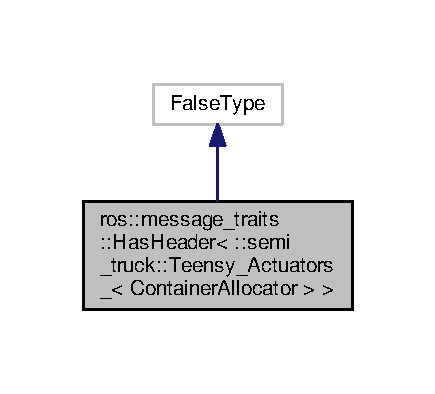
\includegraphics[width=209pt]{structros_1_1message__traits_1_1_has_header_3_01_1_1semi__truck_1_1_teensy___actuators___3_01_co18eb1472522127f29dda17275cdd5b27}
\end{center}
\end{figure}


Collaboration diagram for ros\+:\+:message\+\_\+traits\+:\+:Has\+Header$<$ \+:\+:semi\+\_\+truck\+:\+:Teensy\+\_\+\+Actuators\+\_\+$<$ Container\+Allocator $>$ $>$\+:\nopagebreak
\begin{figure}[H]
\begin{center}
\leavevmode
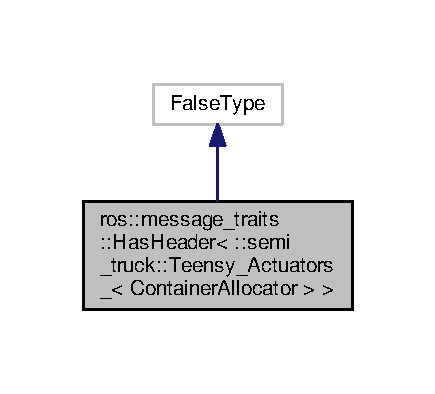
\includegraphics[width=209pt]{structros_1_1message__traits_1_1_has_header_3_01_1_1semi__truck_1_1_teensy___actuators___3_01_cobb41f2262ef52d212439be3a2bb589cf}
\end{center}
\end{figure}


The documentation for this struct was generated from the following file\+:\begin{DoxyCompactItemize}
\item 
daimtronics/semi\+\_\+catkin\+\_\+ws/src/semi\+\_\+truck/include/\hyperlink{_teensy___actuators_8h}{Teensy\+\_\+\+Actuators.\+h}\end{DoxyCompactItemize}

\hypertarget{structros_1_1message__traits_1_1_has_header_3_01_1_1semi__truck_1_1_teensy___actuators___3_01_coe86513e6694fc989720644eb04b2c486}{}\section{ros\+:\+:message\+\_\+traits\+:\+:Has\+Header$<$ \+:\+:semi\+\_\+truck\+:\+:Teensy\+\_\+\+Actuators\+\_\+$<$ Container\+Allocator $>$ const $>$ Struct Template Reference}
\label{structros_1_1message__traits_1_1_has_header_3_01_1_1semi__truck_1_1_teensy___actuators___3_01_coe86513e6694fc989720644eb04b2c486}\index{ros\+::message\+\_\+traits\+::\+Has\+Header$<$ \+::semi\+\_\+truck\+::\+Teensy\+\_\+\+Actuators\+\_\+$<$ Container\+Allocator $>$ const  $>$@{ros\+::message\+\_\+traits\+::\+Has\+Header$<$ \+::semi\+\_\+truck\+::\+Teensy\+\_\+\+Actuators\+\_\+$<$ Container\+Allocator $>$ const  $>$}}


{\ttfamily \#include $<$Teensy\+\_\+\+Actuators.\+h$>$}



Inheritance diagram for ros\+:\+:message\+\_\+traits\+:\+:Has\+Header$<$ \+:\+:semi\+\_\+truck\+:\+:Teensy\+\_\+\+Actuators\+\_\+$<$ Container\+Allocator $>$ const $>$\+:\nopagebreak
\begin{figure}[H]
\begin{center}
\leavevmode
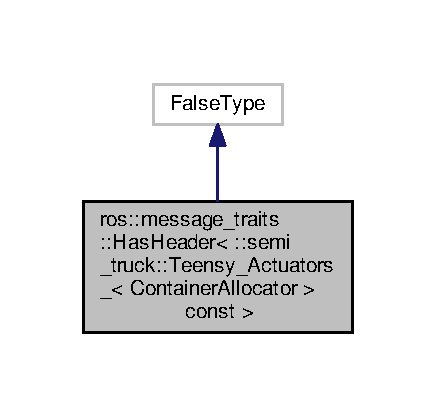
\includegraphics[width=209pt]{structros_1_1message__traits_1_1_has_header_3_01_1_1semi__truck_1_1_teensy___actuators___3_01_co21e737ff7bf090f0bf05daab3f8c4a3d}
\end{center}
\end{figure}


Collaboration diagram for ros\+:\+:message\+\_\+traits\+:\+:Has\+Header$<$ \+:\+:semi\+\_\+truck\+:\+:Teensy\+\_\+\+Actuators\+\_\+$<$ Container\+Allocator $>$ const $>$\+:\nopagebreak
\begin{figure}[H]
\begin{center}
\leavevmode
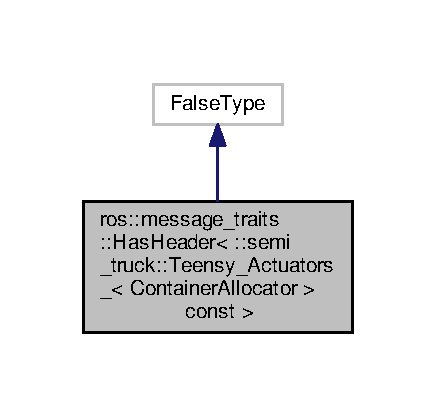
\includegraphics[width=209pt]{structros_1_1message__traits_1_1_has_header_3_01_1_1semi__truck_1_1_teensy___actuators___3_01_coc0dc8493ad8bf7fdbb800952171a3e5d}
\end{center}
\end{figure}


The documentation for this struct was generated from the following file\+:\begin{DoxyCompactItemize}
\item 
daimtronics/semi\+\_\+catkin\+\_\+ws/src/semi\+\_\+truck/include/\hyperlink{_teensy___actuators_8h}{Teensy\+\_\+\+Actuators.\+h}\end{DoxyCompactItemize}

\hypertarget{structros_1_1message__traits_1_1_has_header_3_01_1_1semi__truck_1_1_teensy___sensors___3_01_container_allocator_01_4_01_4}{}\section{ros\+:\+:message\+\_\+traits\+:\+:Has\+Header$<$ \+:\+:semi\+\_\+truck\+:\+:Teensy\+\_\+\+Sensors\+\_\+$<$ Container\+Allocator $>$ $>$ Struct Template Reference}
\label{structros_1_1message__traits_1_1_has_header_3_01_1_1semi__truck_1_1_teensy___sensors___3_01_container_allocator_01_4_01_4}\index{ros\+::message\+\_\+traits\+::\+Has\+Header$<$ \+::semi\+\_\+truck\+::\+Teensy\+\_\+\+Sensors\+\_\+$<$ Container\+Allocator $>$ $>$@{ros\+::message\+\_\+traits\+::\+Has\+Header$<$ \+::semi\+\_\+truck\+::\+Teensy\+\_\+\+Sensors\+\_\+$<$ Container\+Allocator $>$ $>$}}


{\ttfamily \#include $<$Teensy\+\_\+\+Sensors.\+h$>$}



Inheritance diagram for ros\+:\+:message\+\_\+traits\+:\+:Has\+Header$<$ \+:\+:semi\+\_\+truck\+:\+:Teensy\+\_\+\+Sensors\+\_\+$<$ Container\+Allocator $>$ $>$\+:\nopagebreak
\begin{figure}[H]
\begin{center}
\leavevmode
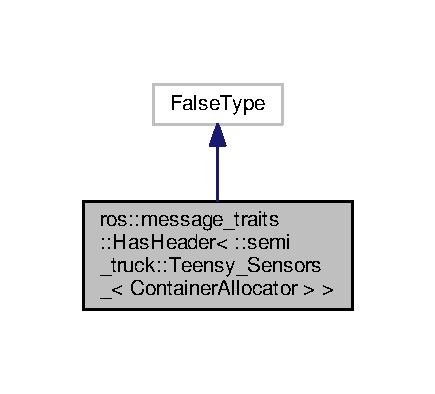
\includegraphics[width=209pt]{structros_1_1message__traits_1_1_has_header_3_01_1_1semi__truck_1_1_teensy___sensors___3_01_cont8409c41542eae9da2f6e341cda4ed823}
\end{center}
\end{figure}


Collaboration diagram for ros\+:\+:message\+\_\+traits\+:\+:Has\+Header$<$ \+:\+:semi\+\_\+truck\+:\+:Teensy\+\_\+\+Sensors\+\_\+$<$ Container\+Allocator $>$ $>$\+:\nopagebreak
\begin{figure}[H]
\begin{center}
\leavevmode
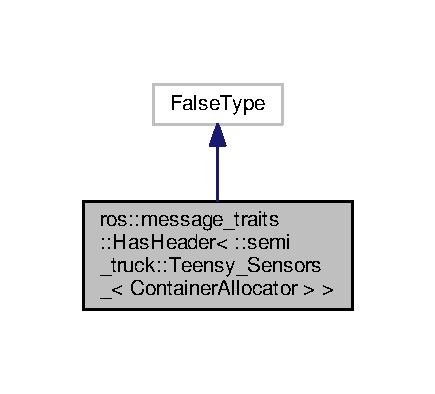
\includegraphics[width=209pt]{structros_1_1message__traits_1_1_has_header_3_01_1_1semi__truck_1_1_teensy___sensors___3_01_cont99a4e8a172ebdec2ee5e1c6f01ac464b}
\end{center}
\end{figure}


The documentation for this struct was generated from the following file\+:\begin{DoxyCompactItemize}
\item 
daimtronics/semi\+\_\+catkin\+\_\+ws/src/semi\+\_\+truck/include/\hyperlink{_teensy___sensors_8h}{Teensy\+\_\+\+Sensors.\+h}\end{DoxyCompactItemize}

\hypertarget{structros_1_1message__traits_1_1_has_header_3_01_1_1semi__truck_1_1_teensy___sensors___3_01_cont27420888fce5a6e96344b08bcfbbf57b}{}\section{ros\+:\+:message\+\_\+traits\+:\+:Has\+Header$<$ \+:\+:semi\+\_\+truck\+:\+:Teensy\+\_\+\+Sensors\+\_\+$<$ Container\+Allocator $>$ const $>$ Struct Template Reference}
\label{structros_1_1message__traits_1_1_has_header_3_01_1_1semi__truck_1_1_teensy___sensors___3_01_cont27420888fce5a6e96344b08bcfbbf57b}\index{ros\+::message\+\_\+traits\+::\+Has\+Header$<$ \+::semi\+\_\+truck\+::\+Teensy\+\_\+\+Sensors\+\_\+$<$ Container\+Allocator $>$ const  $>$@{ros\+::message\+\_\+traits\+::\+Has\+Header$<$ \+::semi\+\_\+truck\+::\+Teensy\+\_\+\+Sensors\+\_\+$<$ Container\+Allocator $>$ const  $>$}}


{\ttfamily \#include $<$Teensy\+\_\+\+Sensors.\+h$>$}



Inheritance diagram for ros\+:\+:message\+\_\+traits\+:\+:Has\+Header$<$ \+:\+:semi\+\_\+truck\+:\+:Teensy\+\_\+\+Sensors\+\_\+$<$ Container\+Allocator $>$ const $>$\+:\nopagebreak
\begin{figure}[H]
\begin{center}
\leavevmode
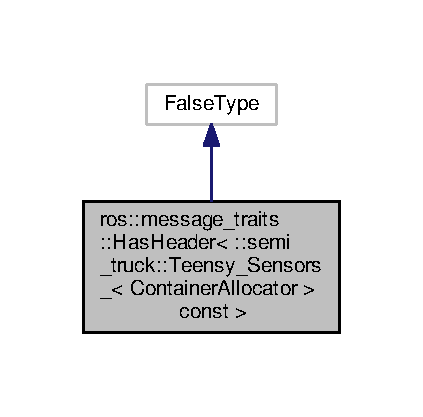
\includegraphics[width=203pt]{structros_1_1message__traits_1_1_has_header_3_01_1_1semi__truck_1_1_teensy___sensors___3_01_contf7f62526d34fd86c71475ca367bd221d}
\end{center}
\end{figure}


Collaboration diagram for ros\+:\+:message\+\_\+traits\+:\+:Has\+Header$<$ \+:\+:semi\+\_\+truck\+:\+:Teensy\+\_\+\+Sensors\+\_\+$<$ Container\+Allocator $>$ const $>$\+:\nopagebreak
\begin{figure}[H]
\begin{center}
\leavevmode
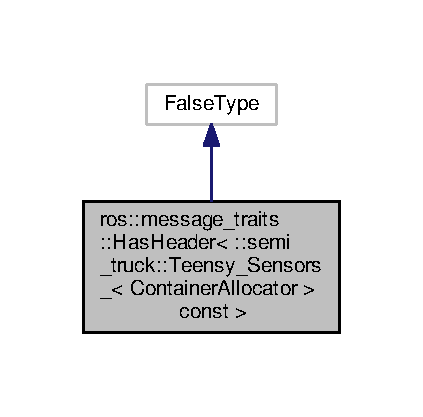
\includegraphics[width=203pt]{structros_1_1message__traits_1_1_has_header_3_01_1_1semi__truck_1_1_teensy___sensors___3_01_cont1388c6e356159dc778a6603983922885}
\end{center}
\end{figure}


The documentation for this struct was generated from the following file\+:\begin{DoxyCompactItemize}
\item 
daimtronics/semi\+\_\+catkin\+\_\+ws/src/semi\+\_\+truck/include/\hyperlink{_teensy___sensors_8h}{Teensy\+\_\+\+Sensors.\+h}\end{DoxyCompactItemize}

\hypertarget{structros_1_1message__traits_1_1_is_fixed_size_3_01_1_1semi__truck_1_1_teensy___actuators___3_01_container_allocator_01_4_01_4}{}\section{ros\+:\+:message\+\_\+traits\+:\+:Is\+Fixed\+Size$<$ \+:\+:semi\+\_\+truck\+:\+:Teensy\+\_\+\+Actuators\+\_\+$<$ Container\+Allocator $>$ $>$ Struct Template Reference}
\label{structros_1_1message__traits_1_1_is_fixed_size_3_01_1_1semi__truck_1_1_teensy___actuators___3_01_container_allocator_01_4_01_4}\index{ros\+::message\+\_\+traits\+::\+Is\+Fixed\+Size$<$ \+::semi\+\_\+truck\+::\+Teensy\+\_\+\+Actuators\+\_\+$<$ Container\+Allocator $>$ $>$@{ros\+::message\+\_\+traits\+::\+Is\+Fixed\+Size$<$ \+::semi\+\_\+truck\+::\+Teensy\+\_\+\+Actuators\+\_\+$<$ Container\+Allocator $>$ $>$}}


{\ttfamily \#include $<$Teensy\+\_\+\+Actuators.\+h$>$}



Inheritance diagram for ros\+:\+:message\+\_\+traits\+:\+:Is\+Fixed\+Size$<$ \+:\+:semi\+\_\+truck\+:\+:Teensy\+\_\+\+Actuators\+\_\+$<$ Container\+Allocator $>$ $>$\+:\nopagebreak
\begin{figure}[H]
\begin{center}
\leavevmode
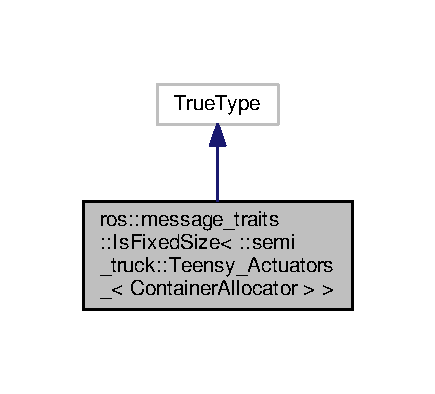
\includegraphics[width=209pt]{structros_1_1message__traits_1_1_is_fixed_size_3_01_1_1semi__truck_1_1_teensy___actuators___3_012a97eaa163c25a98b0c76764d340d2a7}
\end{center}
\end{figure}


Collaboration diagram for ros\+:\+:message\+\_\+traits\+:\+:Is\+Fixed\+Size$<$ \+:\+:semi\+\_\+truck\+:\+:Teensy\+\_\+\+Actuators\+\_\+$<$ Container\+Allocator $>$ $>$\+:\nopagebreak
\begin{figure}[H]
\begin{center}
\leavevmode
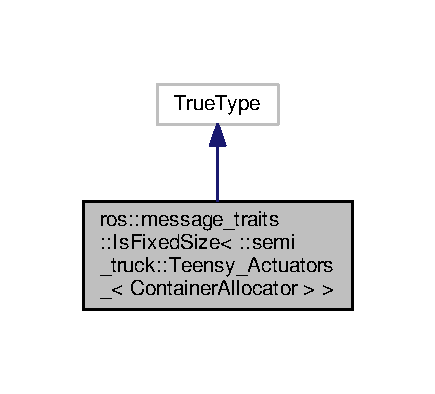
\includegraphics[width=209pt]{structros_1_1message__traits_1_1_is_fixed_size_3_01_1_1semi__truck_1_1_teensy___actuators___3_01837b0845e895ab918142d4b818f0d00e}
\end{center}
\end{figure}


The documentation for this struct was generated from the following file\+:\begin{DoxyCompactItemize}
\item 
daimtronics/semi\+\_\+catkin\+\_\+ws/src/semi\+\_\+truck/include/\hyperlink{_teensy___actuators_8h}{Teensy\+\_\+\+Actuators.\+h}\end{DoxyCompactItemize}

\hypertarget{structros_1_1message__traits_1_1_is_fixed_size_3_01_1_1semi__truck_1_1_teensy___actuators___3_01e88fb587a6d6e04d6a7968cdf33bb127}{}\section{ros\+:\+:message\+\_\+traits\+:\+:Is\+Fixed\+Size$<$ \+:\+:semi\+\_\+truck\+:\+:Teensy\+\_\+\+Actuators\+\_\+$<$ Container\+Allocator $>$ const $>$ Struct Template Reference}
\label{structros_1_1message__traits_1_1_is_fixed_size_3_01_1_1semi__truck_1_1_teensy___actuators___3_01e88fb587a6d6e04d6a7968cdf33bb127}\index{ros\+::message\+\_\+traits\+::\+Is\+Fixed\+Size$<$ \+::semi\+\_\+truck\+::\+Teensy\+\_\+\+Actuators\+\_\+$<$ Container\+Allocator $>$ const  $>$@{ros\+::message\+\_\+traits\+::\+Is\+Fixed\+Size$<$ \+::semi\+\_\+truck\+::\+Teensy\+\_\+\+Actuators\+\_\+$<$ Container\+Allocator $>$ const  $>$}}


{\ttfamily \#include $<$Teensy\+\_\+\+Actuators.\+h$>$}



Inheritance diagram for ros\+:\+:message\+\_\+traits\+:\+:Is\+Fixed\+Size$<$ \+:\+:semi\+\_\+truck\+:\+:Teensy\+\_\+\+Actuators\+\_\+$<$ Container\+Allocator $>$ const $>$\+:\nopagebreak
\begin{figure}[H]
\begin{center}
\leavevmode
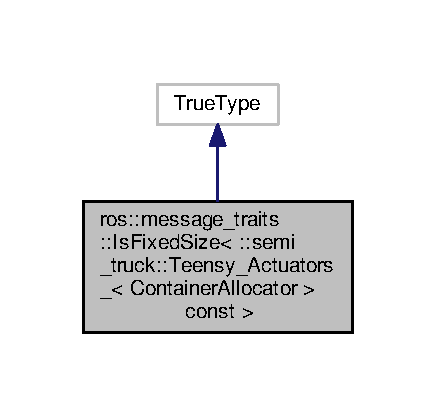
\includegraphics[width=209pt]{structros_1_1message__traits_1_1_is_fixed_size_3_01_1_1semi__truck_1_1_teensy___actuators___3_01a04aa7b95ef0ff2957962baed1b65541}
\end{center}
\end{figure}


Collaboration diagram for ros\+:\+:message\+\_\+traits\+:\+:Is\+Fixed\+Size$<$ \+:\+:semi\+\_\+truck\+:\+:Teensy\+\_\+\+Actuators\+\_\+$<$ Container\+Allocator $>$ const $>$\+:\nopagebreak
\begin{figure}[H]
\begin{center}
\leavevmode
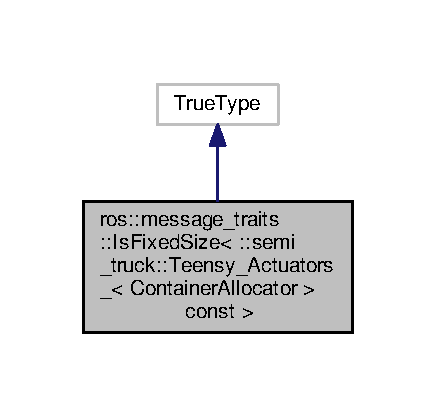
\includegraphics[width=209pt]{structros_1_1message__traits_1_1_is_fixed_size_3_01_1_1semi__truck_1_1_teensy___actuators___3_01549018ee433734dfb23afefae8aebc19}
\end{center}
\end{figure}


The documentation for this struct was generated from the following file\+:\begin{DoxyCompactItemize}
\item 
daimtronics/semi\+\_\+catkin\+\_\+ws/src/semi\+\_\+truck/include/\hyperlink{_teensy___actuators_8h}{Teensy\+\_\+\+Actuators.\+h}\end{DoxyCompactItemize}

\hypertarget{structros_1_1message__traits_1_1_is_fixed_size_3_01_1_1semi__truck_1_1_teensy___sensors___3_01_container_allocator_01_4_01_4}{}\section{ros\+:\+:message\+\_\+traits\+:\+:Is\+Fixed\+Size$<$ \+:\+:semi\+\_\+truck\+:\+:Teensy\+\_\+\+Sensors\+\_\+$<$ Container\+Allocator $>$ $>$ Struct Template Reference}
\label{structros_1_1message__traits_1_1_is_fixed_size_3_01_1_1semi__truck_1_1_teensy___sensors___3_01_container_allocator_01_4_01_4}\index{ros\+::message\+\_\+traits\+::\+Is\+Fixed\+Size$<$ \+::semi\+\_\+truck\+::\+Teensy\+\_\+\+Sensors\+\_\+$<$ Container\+Allocator $>$ $>$@{ros\+::message\+\_\+traits\+::\+Is\+Fixed\+Size$<$ \+::semi\+\_\+truck\+::\+Teensy\+\_\+\+Sensors\+\_\+$<$ Container\+Allocator $>$ $>$}}


{\ttfamily \#include $<$Teensy\+\_\+\+Sensors.\+h$>$}



Inheritance diagram for ros\+:\+:message\+\_\+traits\+:\+:Is\+Fixed\+Size$<$ \+:\+:semi\+\_\+truck\+:\+:Teensy\+\_\+\+Sensors\+\_\+$<$ Container\+Allocator $>$ $>$\+:\nopagebreak
\begin{figure}[H]
\begin{center}
\leavevmode
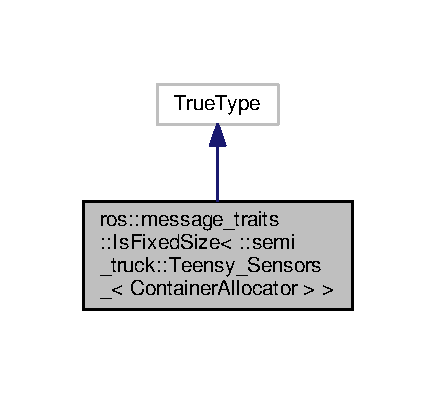
\includegraphics[width=209pt]{structros_1_1message__traits_1_1_is_fixed_size_3_01_1_1semi__truck_1_1_teensy___sensors___3_01_ca610f05107398a23779c2cf5a2710d4f}
\end{center}
\end{figure}


Collaboration diagram for ros\+:\+:message\+\_\+traits\+:\+:Is\+Fixed\+Size$<$ \+:\+:semi\+\_\+truck\+:\+:Teensy\+\_\+\+Sensors\+\_\+$<$ Container\+Allocator $>$ $>$\+:\nopagebreak
\begin{figure}[H]
\begin{center}
\leavevmode
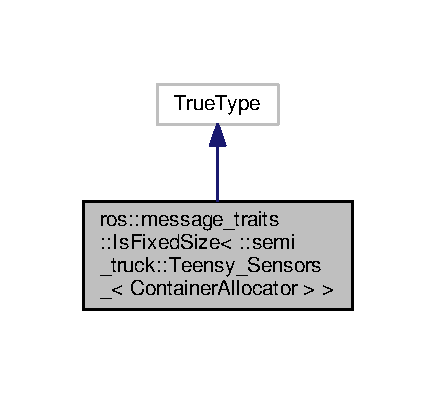
\includegraphics[width=209pt]{structros_1_1message__traits_1_1_is_fixed_size_3_01_1_1semi__truck_1_1_teensy___sensors___3_01_c291bb9ff93cc810544d8e334bf4d8ed7}
\end{center}
\end{figure}


The documentation for this struct was generated from the following file\+:\begin{DoxyCompactItemize}
\item 
daimtronics/semi\+\_\+catkin\+\_\+ws/src/semi\+\_\+truck/include/\hyperlink{_teensy___sensors_8h}{Teensy\+\_\+\+Sensors.\+h}\end{DoxyCompactItemize}

\hypertarget{structros_1_1message__traits_1_1_is_fixed_size_3_01_1_1semi__truck_1_1_teensy___sensors___3_01_cb53d5848a141775744a1974dc7127755}{}\section{ros\+:\+:message\+\_\+traits\+:\+:Is\+Fixed\+Size$<$ \+:\+:semi\+\_\+truck\+:\+:Teensy\+\_\+\+Sensors\+\_\+$<$ Container\+Allocator $>$ const $>$ Struct Template Reference}
\label{structros_1_1message__traits_1_1_is_fixed_size_3_01_1_1semi__truck_1_1_teensy___sensors___3_01_cb53d5848a141775744a1974dc7127755}\index{ros\+::message\+\_\+traits\+::\+Is\+Fixed\+Size$<$ \+::semi\+\_\+truck\+::\+Teensy\+\_\+\+Sensors\+\_\+$<$ Container\+Allocator $>$ const  $>$@{ros\+::message\+\_\+traits\+::\+Is\+Fixed\+Size$<$ \+::semi\+\_\+truck\+::\+Teensy\+\_\+\+Sensors\+\_\+$<$ Container\+Allocator $>$ const  $>$}}


{\ttfamily \#include $<$Teensy\+\_\+\+Sensors.\+h$>$}



Inheritance diagram for ros\+:\+:message\+\_\+traits\+:\+:Is\+Fixed\+Size$<$ \+:\+:semi\+\_\+truck\+:\+:Teensy\+\_\+\+Sensors\+\_\+$<$ Container\+Allocator $>$ const $>$\+:\nopagebreak
\begin{figure}[H]
\begin{center}
\leavevmode
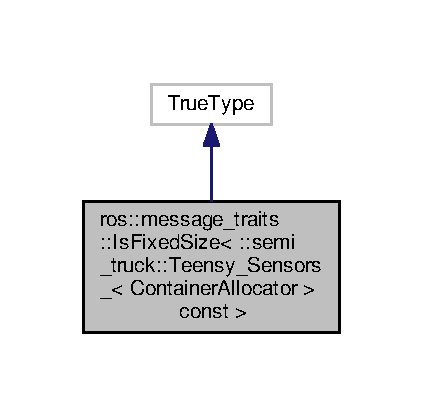
\includegraphics[width=203pt]{structros_1_1message__traits_1_1_is_fixed_size_3_01_1_1semi__truck_1_1_teensy___sensors___3_01_cbfa71abce16c9c1adb8a197a0358ffd5}
\end{center}
\end{figure}


Collaboration diagram for ros\+:\+:message\+\_\+traits\+:\+:Is\+Fixed\+Size$<$ \+:\+:semi\+\_\+truck\+:\+:Teensy\+\_\+\+Sensors\+\_\+$<$ Container\+Allocator $>$ const $>$\+:\nopagebreak
\begin{figure}[H]
\begin{center}
\leavevmode
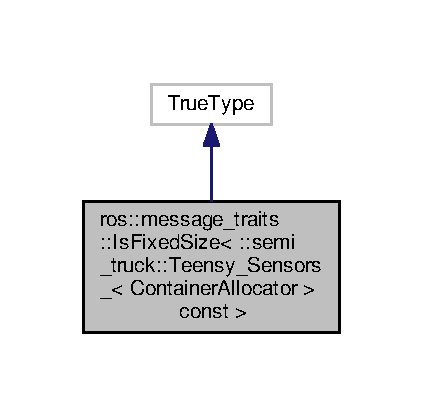
\includegraphics[width=203pt]{structros_1_1message__traits_1_1_is_fixed_size_3_01_1_1semi__truck_1_1_teensy___sensors___3_01_cb1921b0987cc8a964f9a9efc7494c7a8}
\end{center}
\end{figure}


The documentation for this struct was generated from the following file\+:\begin{DoxyCompactItemize}
\item 
daimtronics/semi\+\_\+catkin\+\_\+ws/src/semi\+\_\+truck/include/\hyperlink{_teensy___sensors_8h}{Teensy\+\_\+\+Sensors.\+h}\end{DoxyCompactItemize}

\hypertarget{structros_1_1message__traits_1_1_is_message_3_01_1_1semi__truck_1_1_teensy___actuators___3_01_container_allocator_01_4_01_4}{}\section{ros\+:\+:message\+\_\+traits\+:\+:Is\+Message$<$ \+:\+:semi\+\_\+truck\+:\+:Teensy\+\_\+\+Actuators\+\_\+$<$ Container\+Allocator $>$ $>$ Struct Template Reference}
\label{structros_1_1message__traits_1_1_is_message_3_01_1_1semi__truck_1_1_teensy___actuators___3_01_container_allocator_01_4_01_4}\index{ros\+::message\+\_\+traits\+::\+Is\+Message$<$ \+::semi\+\_\+truck\+::\+Teensy\+\_\+\+Actuators\+\_\+$<$ Container\+Allocator $>$ $>$@{ros\+::message\+\_\+traits\+::\+Is\+Message$<$ \+::semi\+\_\+truck\+::\+Teensy\+\_\+\+Actuators\+\_\+$<$ Container\+Allocator $>$ $>$}}


{\ttfamily \#include $<$Teensy\+\_\+\+Actuators.\+h$>$}



Inheritance diagram for ros\+:\+:message\+\_\+traits\+:\+:Is\+Message$<$ \+:\+:semi\+\_\+truck\+:\+:Teensy\+\_\+\+Actuators\+\_\+$<$ Container\+Allocator $>$ $>$\+:\nopagebreak
\begin{figure}[H]
\begin{center}
\leavevmode
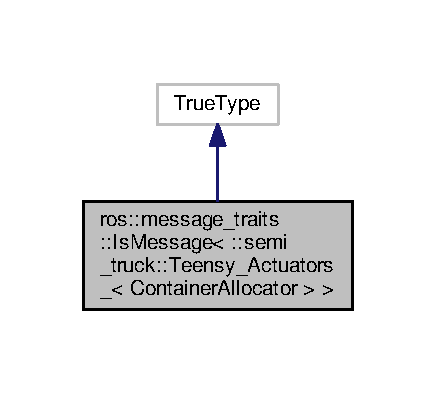
\includegraphics[width=209pt]{structros_1_1message__traits_1_1_is_message_3_01_1_1semi__truck_1_1_teensy___actuators___3_01_cod0b1811ec24b19ee705cad8bd2f007d0}
\end{center}
\end{figure}


Collaboration diagram for ros\+:\+:message\+\_\+traits\+:\+:Is\+Message$<$ \+:\+:semi\+\_\+truck\+:\+:Teensy\+\_\+\+Actuators\+\_\+$<$ Container\+Allocator $>$ $>$\+:\nopagebreak
\begin{figure}[H]
\begin{center}
\leavevmode
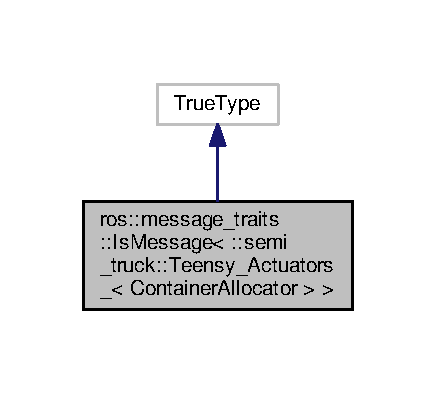
\includegraphics[width=209pt]{structros_1_1message__traits_1_1_is_message_3_01_1_1semi__truck_1_1_teensy___actuators___3_01_co34e3ece18aa437021b17263e8335e268}
\end{center}
\end{figure}


The documentation for this struct was generated from the following file\+:\begin{DoxyCompactItemize}
\item 
daimtronics/semi\+\_\+catkin\+\_\+ws/src/semi\+\_\+truck/include/\hyperlink{_teensy___actuators_8h}{Teensy\+\_\+\+Actuators.\+h}\end{DoxyCompactItemize}

\hypertarget{structros_1_1message__traits_1_1_is_message_3_01_1_1semi__truck_1_1_teensy___actuators___3_01_cobc29fbe598d16bac74a311be55406c9e}{}\section{ros\+:\+:message\+\_\+traits\+:\+:Is\+Message$<$ \+:\+:semi\+\_\+truck\+:\+:Teensy\+\_\+\+Actuators\+\_\+$<$ Container\+Allocator $>$ const $>$ Struct Template Reference}
\label{structros_1_1message__traits_1_1_is_message_3_01_1_1semi__truck_1_1_teensy___actuators___3_01_cobc29fbe598d16bac74a311be55406c9e}\index{ros\+::message\+\_\+traits\+::\+Is\+Message$<$ \+::semi\+\_\+truck\+::\+Teensy\+\_\+\+Actuators\+\_\+$<$ Container\+Allocator $>$ const  $>$@{ros\+::message\+\_\+traits\+::\+Is\+Message$<$ \+::semi\+\_\+truck\+::\+Teensy\+\_\+\+Actuators\+\_\+$<$ Container\+Allocator $>$ const  $>$}}


{\ttfamily \#include $<$Teensy\+\_\+\+Actuators.\+h$>$}



Inheritance diagram for ros\+:\+:message\+\_\+traits\+:\+:Is\+Message$<$ \+:\+:semi\+\_\+truck\+:\+:Teensy\+\_\+\+Actuators\+\_\+$<$ Container\+Allocator $>$ const $>$\+:\nopagebreak
\begin{figure}[H]
\begin{center}
\leavevmode
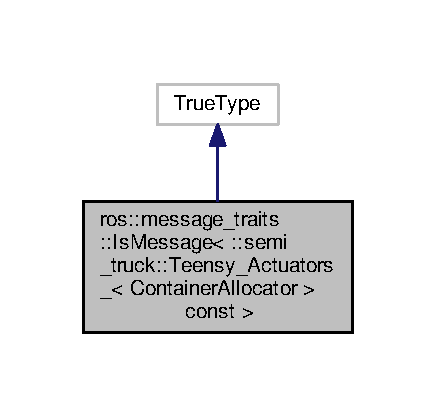
\includegraphics[width=209pt]{structros_1_1message__traits_1_1_is_message_3_01_1_1semi__truck_1_1_teensy___actuators___3_01_co7825622c43c361e8e6549116ac595292}
\end{center}
\end{figure}


Collaboration diagram for ros\+:\+:message\+\_\+traits\+:\+:Is\+Message$<$ \+:\+:semi\+\_\+truck\+:\+:Teensy\+\_\+\+Actuators\+\_\+$<$ Container\+Allocator $>$ const $>$\+:\nopagebreak
\begin{figure}[H]
\begin{center}
\leavevmode
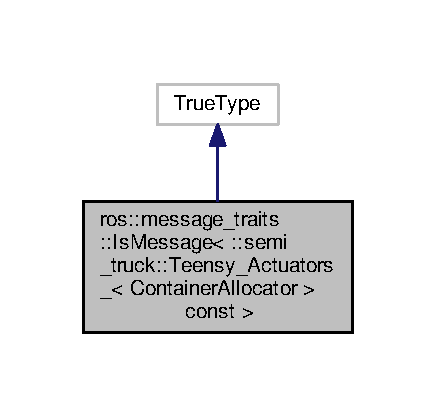
\includegraphics[width=209pt]{structros_1_1message__traits_1_1_is_message_3_01_1_1semi__truck_1_1_teensy___actuators___3_01_co6df848739a639501dddc4a4521597a36}
\end{center}
\end{figure}


The documentation for this struct was generated from the following file\+:\begin{DoxyCompactItemize}
\item 
daimtronics/semi\+\_\+catkin\+\_\+ws/src/semi\+\_\+truck/include/\hyperlink{_teensy___actuators_8h}{Teensy\+\_\+\+Actuators.\+h}\end{DoxyCompactItemize}

\hypertarget{structros_1_1message__traits_1_1_is_message_3_01_1_1semi__truck_1_1_teensy___sensors___3_01_container_allocator_01_4_01_4}{}\section{ros\+:\+:message\+\_\+traits\+:\+:Is\+Message$<$ \+:\+:semi\+\_\+truck\+:\+:Teensy\+\_\+\+Sensors\+\_\+$<$ Container\+Allocator $>$ $>$ Struct Template Reference}
\label{structros_1_1message__traits_1_1_is_message_3_01_1_1semi__truck_1_1_teensy___sensors___3_01_container_allocator_01_4_01_4}\index{ros\+::message\+\_\+traits\+::\+Is\+Message$<$ \+::semi\+\_\+truck\+::\+Teensy\+\_\+\+Sensors\+\_\+$<$ Container\+Allocator $>$ $>$@{ros\+::message\+\_\+traits\+::\+Is\+Message$<$ \+::semi\+\_\+truck\+::\+Teensy\+\_\+\+Sensors\+\_\+$<$ Container\+Allocator $>$ $>$}}


{\ttfamily \#include $<$Teensy\+\_\+\+Sensors.\+h$>$}



Inheritance diagram for ros\+:\+:message\+\_\+traits\+:\+:Is\+Message$<$ \+:\+:semi\+\_\+truck\+:\+:Teensy\+\_\+\+Sensors\+\_\+$<$ Container\+Allocator $>$ $>$\+:\nopagebreak
\begin{figure}[H]
\begin{center}
\leavevmode
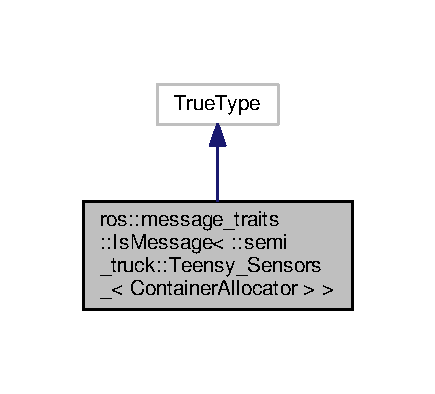
\includegraphics[width=209pt]{structros_1_1message__traits_1_1_is_message_3_01_1_1semi__truck_1_1_teensy___sensors___3_01_cont9e1a5ff2d66359a7a04aa73a00de25c6}
\end{center}
\end{figure}


Collaboration diagram for ros\+:\+:message\+\_\+traits\+:\+:Is\+Message$<$ \+:\+:semi\+\_\+truck\+:\+:Teensy\+\_\+\+Sensors\+\_\+$<$ Container\+Allocator $>$ $>$\+:\nopagebreak
\begin{figure}[H]
\begin{center}
\leavevmode
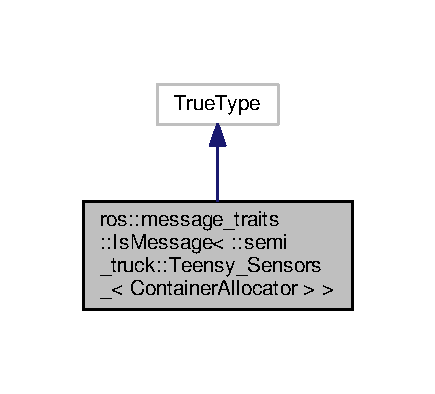
\includegraphics[width=209pt]{structros_1_1message__traits_1_1_is_message_3_01_1_1semi__truck_1_1_teensy___sensors___3_01_conta8f321bc4f924589498a449bfd539cd7}
\end{center}
\end{figure}


The documentation for this struct was generated from the following file\+:\begin{DoxyCompactItemize}
\item 
daimtronics/semi\+\_\+catkin\+\_\+ws/src/semi\+\_\+truck/include/\hyperlink{_teensy___sensors_8h}{Teensy\+\_\+\+Sensors.\+h}\end{DoxyCompactItemize}

\hypertarget{structros_1_1message__traits_1_1_is_message_3_01_1_1semi__truck_1_1_teensy___sensors___3_01_contee20f324312af52498809118a40cc274}{}\section{ros\+:\+:message\+\_\+traits\+:\+:Is\+Message$<$ \+:\+:semi\+\_\+truck\+:\+:Teensy\+\_\+\+Sensors\+\_\+$<$ Container\+Allocator $>$ const $>$ Struct Template Reference}
\label{structros_1_1message__traits_1_1_is_message_3_01_1_1semi__truck_1_1_teensy___sensors___3_01_contee20f324312af52498809118a40cc274}\index{ros\+::message\+\_\+traits\+::\+Is\+Message$<$ \+::semi\+\_\+truck\+::\+Teensy\+\_\+\+Sensors\+\_\+$<$ Container\+Allocator $>$ const  $>$@{ros\+::message\+\_\+traits\+::\+Is\+Message$<$ \+::semi\+\_\+truck\+::\+Teensy\+\_\+\+Sensors\+\_\+$<$ Container\+Allocator $>$ const  $>$}}


{\ttfamily \#include $<$Teensy\+\_\+\+Sensors.\+h$>$}



Inheritance diagram for ros\+:\+:message\+\_\+traits\+:\+:Is\+Message$<$ \+:\+:semi\+\_\+truck\+:\+:Teensy\+\_\+\+Sensors\+\_\+$<$ Container\+Allocator $>$ const $>$\+:\nopagebreak
\begin{figure}[H]
\begin{center}
\leavevmode
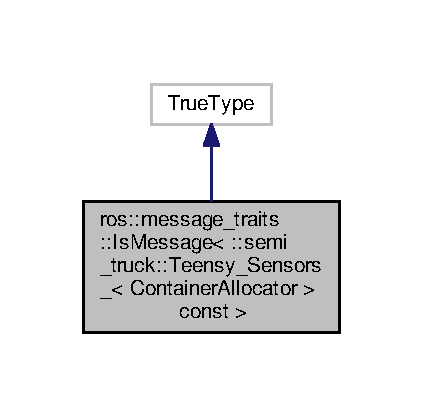
\includegraphics[width=203pt]{structros_1_1message__traits_1_1_is_message_3_01_1_1semi__truck_1_1_teensy___sensors___3_01_cont8602985026d3fce4a20e6339888db709}
\end{center}
\end{figure}


Collaboration diagram for ros\+:\+:message\+\_\+traits\+:\+:Is\+Message$<$ \+:\+:semi\+\_\+truck\+:\+:Teensy\+\_\+\+Sensors\+\_\+$<$ Container\+Allocator $>$ const $>$\+:\nopagebreak
\begin{figure}[H]
\begin{center}
\leavevmode
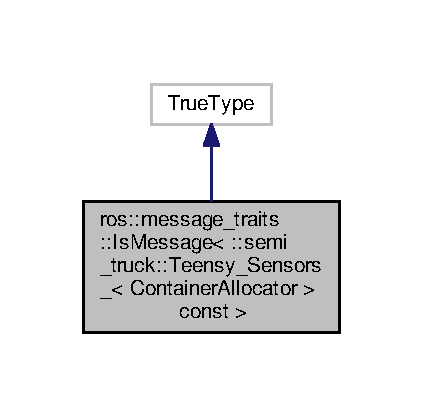
\includegraphics[width=203pt]{structros_1_1message__traits_1_1_is_message_3_01_1_1semi__truck_1_1_teensy___sensors___3_01_cont42eab6994307cc549083cfcb31853bee}
\end{center}
\end{figure}


The documentation for this struct was generated from the following file\+:\begin{DoxyCompactItemize}
\item 
daimtronics/semi\+\_\+catkin\+\_\+ws/src/semi\+\_\+truck/include/\hyperlink{_teensy___sensors_8h}{Teensy\+\_\+\+Sensors.\+h}\end{DoxyCompactItemize}

\hypertarget{structros_1_1message__traits_1_1_m_d5_sum_3_01_1_1semi__truck_1_1_teensy___actuators___3_01_container_allocator_01_4_01_4}{}\section{ros\+:\+:message\+\_\+traits\+:\+:M\+D5\+Sum$<$ \+:\+:semi\+\_\+truck\+:\+:Teensy\+\_\+\+Actuators\+\_\+$<$ Container\+Allocator $>$ $>$ Struct Template Reference}
\label{structros_1_1message__traits_1_1_m_d5_sum_3_01_1_1semi__truck_1_1_teensy___actuators___3_01_container_allocator_01_4_01_4}\index{ros\+::message\+\_\+traits\+::\+M\+D5\+Sum$<$ \+::semi\+\_\+truck\+::\+Teensy\+\_\+\+Actuators\+\_\+$<$ Container\+Allocator $>$ $>$@{ros\+::message\+\_\+traits\+::\+M\+D5\+Sum$<$ \+::semi\+\_\+truck\+::\+Teensy\+\_\+\+Actuators\+\_\+$<$ Container\+Allocator $>$ $>$}}


{\ttfamily \#include $<$Teensy\+\_\+\+Actuators.\+h$>$}

\subsection*{Static Public Member Functions}
\begin{DoxyCompactItemize}
\item 
static const char $\ast$ \hyperlink{structros_1_1message__traits_1_1_m_d5_sum_3_01_1_1semi__truck_1_1_teensy___actuators___3_01_container_allocator_01_4_01_4_a13758bc5f7f2d9783a28af50ec67affe}{value} ()
\item 
static const char $\ast$ \hyperlink{structros_1_1message__traits_1_1_m_d5_sum_3_01_1_1semi__truck_1_1_teensy___actuators___3_01_container_allocator_01_4_01_4_ac7a5562fb2f1a6c78a7a3248b7465d6e}{value} (const \+::\hyperlink{structsemi__truck_1_1_teensy___actuators__}{semi\+\_\+truck\+::\+Teensy\+\_\+\+Actuators\+\_\+}$<$ Container\+Allocator $>$ \&)
\end{DoxyCompactItemize}
\subsection*{Static Public Attributes}
\begin{DoxyCompactItemize}
\item 
static const uint64\+\_\+t \hyperlink{structros_1_1message__traits_1_1_m_d5_sum_3_01_1_1semi__truck_1_1_teensy___actuators___3_01_container_allocator_01_4_01_4_a3b7b6fb0b62486fc31e42a45a16fd3c1}{static\+\_\+value1} = 0x0d131da7355e429d\+U\+LL
\item 
static const uint64\+\_\+t \hyperlink{structros_1_1message__traits_1_1_m_d5_sum_3_01_1_1semi__truck_1_1_teensy___actuators___3_01_container_allocator_01_4_01_4_a9fd6a5beaa08b9601b1f2af0f1528164}{static\+\_\+value2} = 0x9d8b9cc6b2375149\+U\+LL
\end{DoxyCompactItemize}


\subsection{Member Function Documentation}
\index{ros\+::message\+\_\+traits\+::\+M\+D5\+Sum$<$ \+::semi\+\_\+truck\+::\+Teensy\+\_\+\+Actuators\+\_\+$<$ Container\+Allocator $>$ $>$@{ros\+::message\+\_\+traits\+::\+M\+D5\+Sum$<$ \+::semi\+\_\+truck\+::\+Teensy\+\_\+\+Actuators\+\_\+$<$ Container\+Allocator $>$ $>$}!value@{value}}
\index{value@{value}!ros\+::message\+\_\+traits\+::\+M\+D5\+Sum$<$ \+::semi\+\_\+truck\+::\+Teensy\+\_\+\+Actuators\+\_\+$<$ Container\+Allocator $>$ $>$@{ros\+::message\+\_\+traits\+::\+M\+D5\+Sum$<$ \+::semi\+\_\+truck\+::\+Teensy\+\_\+\+Actuators\+\_\+$<$ Container\+Allocator $>$ $>$}}
\subsubsection[{\texorpdfstring{value()}{value()}}]{\setlength{\rightskip}{0pt plus 5cm}template$<$class Container\+Allocator $>$ static const char$\ast$ ros\+::message\+\_\+traits\+::\+M\+D5\+Sum$<$ \+::{\bf semi\+\_\+truck\+::\+Teensy\+\_\+\+Actuators\+\_\+}$<$ Container\+Allocator $>$ $>$\+::value (
\begin{DoxyParamCaption}
{}
\end{DoxyParamCaption}
)\hspace{0.3cm}{\ttfamily [inline]}, {\ttfamily [static]}}\hypertarget{structros_1_1message__traits_1_1_m_d5_sum_3_01_1_1semi__truck_1_1_teensy___actuators___3_01_container_allocator_01_4_01_4_a13758bc5f7f2d9783a28af50ec67affe}{}\label{structros_1_1message__traits_1_1_m_d5_sum_3_01_1_1semi__truck_1_1_teensy___actuators___3_01_container_allocator_01_4_01_4_a13758bc5f7f2d9783a28af50ec67affe}
\index{ros\+::message\+\_\+traits\+::\+M\+D5\+Sum$<$ \+::semi\+\_\+truck\+::\+Teensy\+\_\+\+Actuators\+\_\+$<$ Container\+Allocator $>$ $>$@{ros\+::message\+\_\+traits\+::\+M\+D5\+Sum$<$ \+::semi\+\_\+truck\+::\+Teensy\+\_\+\+Actuators\+\_\+$<$ Container\+Allocator $>$ $>$}!value@{value}}
\index{value@{value}!ros\+::message\+\_\+traits\+::\+M\+D5\+Sum$<$ \+::semi\+\_\+truck\+::\+Teensy\+\_\+\+Actuators\+\_\+$<$ Container\+Allocator $>$ $>$@{ros\+::message\+\_\+traits\+::\+M\+D5\+Sum$<$ \+::semi\+\_\+truck\+::\+Teensy\+\_\+\+Actuators\+\_\+$<$ Container\+Allocator $>$ $>$}}
\subsubsection[{\texorpdfstring{value(const \+::semi\+\_\+truck\+::\+Teensy\+\_\+\+Actuators\+\_\+$<$ Container\+Allocator $>$ \&)}{value(const ::semi_truck::Teensy_Actuators_< ContainerAllocator > &)}}]{\setlength{\rightskip}{0pt plus 5cm}template$<$class Container\+Allocator $>$ static const char$\ast$ ros\+::message\+\_\+traits\+::\+M\+D5\+Sum$<$ \+::{\bf semi\+\_\+truck\+::\+Teensy\+\_\+\+Actuators\+\_\+}$<$ Container\+Allocator $>$ $>$\+::value (
\begin{DoxyParamCaption}
\item[{const \+::{\bf semi\+\_\+truck\+::\+Teensy\+\_\+\+Actuators\+\_\+}$<$ Container\+Allocator $>$ \&}]{}
\end{DoxyParamCaption}
)\hspace{0.3cm}{\ttfamily [inline]}, {\ttfamily [static]}}\hypertarget{structros_1_1message__traits_1_1_m_d5_sum_3_01_1_1semi__truck_1_1_teensy___actuators___3_01_container_allocator_01_4_01_4_ac7a5562fb2f1a6c78a7a3248b7465d6e}{}\label{structros_1_1message__traits_1_1_m_d5_sum_3_01_1_1semi__truck_1_1_teensy___actuators___3_01_container_allocator_01_4_01_4_ac7a5562fb2f1a6c78a7a3248b7465d6e}


\subsection{Member Data Documentation}
\index{ros\+::message\+\_\+traits\+::\+M\+D5\+Sum$<$ \+::semi\+\_\+truck\+::\+Teensy\+\_\+\+Actuators\+\_\+$<$ Container\+Allocator $>$ $>$@{ros\+::message\+\_\+traits\+::\+M\+D5\+Sum$<$ \+::semi\+\_\+truck\+::\+Teensy\+\_\+\+Actuators\+\_\+$<$ Container\+Allocator $>$ $>$}!static\+\_\+value1@{static\+\_\+value1}}
\index{static\+\_\+value1@{static\+\_\+value1}!ros\+::message\+\_\+traits\+::\+M\+D5\+Sum$<$ \+::semi\+\_\+truck\+::\+Teensy\+\_\+\+Actuators\+\_\+$<$ Container\+Allocator $>$ $>$@{ros\+::message\+\_\+traits\+::\+M\+D5\+Sum$<$ \+::semi\+\_\+truck\+::\+Teensy\+\_\+\+Actuators\+\_\+$<$ Container\+Allocator $>$ $>$}}
\subsubsection[{\texorpdfstring{static\+\_\+value1}{static_value1}}]{\setlength{\rightskip}{0pt plus 5cm}template$<$class Container\+Allocator $>$ const uint64\+\_\+t ros\+::message\+\_\+traits\+::\+M\+D5\+Sum$<$ \+::{\bf semi\+\_\+truck\+::\+Teensy\+\_\+\+Actuators\+\_\+}$<$ Container\+Allocator $>$ $>$\+::static\+\_\+value1 = 0x0d131da7355e429d\+U\+LL\hspace{0.3cm}{\ttfamily [static]}}\hypertarget{structros_1_1message__traits_1_1_m_d5_sum_3_01_1_1semi__truck_1_1_teensy___actuators___3_01_container_allocator_01_4_01_4_a3b7b6fb0b62486fc31e42a45a16fd3c1}{}\label{structros_1_1message__traits_1_1_m_d5_sum_3_01_1_1semi__truck_1_1_teensy___actuators___3_01_container_allocator_01_4_01_4_a3b7b6fb0b62486fc31e42a45a16fd3c1}
\index{ros\+::message\+\_\+traits\+::\+M\+D5\+Sum$<$ \+::semi\+\_\+truck\+::\+Teensy\+\_\+\+Actuators\+\_\+$<$ Container\+Allocator $>$ $>$@{ros\+::message\+\_\+traits\+::\+M\+D5\+Sum$<$ \+::semi\+\_\+truck\+::\+Teensy\+\_\+\+Actuators\+\_\+$<$ Container\+Allocator $>$ $>$}!static\+\_\+value2@{static\+\_\+value2}}
\index{static\+\_\+value2@{static\+\_\+value2}!ros\+::message\+\_\+traits\+::\+M\+D5\+Sum$<$ \+::semi\+\_\+truck\+::\+Teensy\+\_\+\+Actuators\+\_\+$<$ Container\+Allocator $>$ $>$@{ros\+::message\+\_\+traits\+::\+M\+D5\+Sum$<$ \+::semi\+\_\+truck\+::\+Teensy\+\_\+\+Actuators\+\_\+$<$ Container\+Allocator $>$ $>$}}
\subsubsection[{\texorpdfstring{static\+\_\+value2}{static_value2}}]{\setlength{\rightskip}{0pt plus 5cm}template$<$class Container\+Allocator $>$ const uint64\+\_\+t ros\+::message\+\_\+traits\+::\+M\+D5\+Sum$<$ \+::{\bf semi\+\_\+truck\+::\+Teensy\+\_\+\+Actuators\+\_\+}$<$ Container\+Allocator $>$ $>$\+::static\+\_\+value2 = 0x9d8b9cc6b2375149\+U\+LL\hspace{0.3cm}{\ttfamily [static]}}\hypertarget{structros_1_1message__traits_1_1_m_d5_sum_3_01_1_1semi__truck_1_1_teensy___actuators___3_01_container_allocator_01_4_01_4_a9fd6a5beaa08b9601b1f2af0f1528164}{}\label{structros_1_1message__traits_1_1_m_d5_sum_3_01_1_1semi__truck_1_1_teensy___actuators___3_01_container_allocator_01_4_01_4_a9fd6a5beaa08b9601b1f2af0f1528164}


The documentation for this struct was generated from the following file\+:\begin{DoxyCompactItemize}
\item 
daimtronics/semi\+\_\+catkin\+\_\+ws/src/semi\+\_\+truck/include/\hyperlink{_teensy___actuators_8h}{Teensy\+\_\+\+Actuators.\+h}\end{DoxyCompactItemize}

\hypertarget{structros_1_1message__traits_1_1_m_d5_sum_3_01_1_1semi__truck_1_1_teensy___sensors___3_01_container_allocator_01_4_01_4}{}\section{ros\+:\+:message\+\_\+traits\+:\+:M\+D5\+Sum$<$ \+:\+:semi\+\_\+truck\+:\+:Teensy\+\_\+\+Sensors\+\_\+$<$ Container\+Allocator $>$ $>$ Struct Template Reference}
\label{structros_1_1message__traits_1_1_m_d5_sum_3_01_1_1semi__truck_1_1_teensy___sensors___3_01_container_allocator_01_4_01_4}\index{ros\+::message\+\_\+traits\+::\+M\+D5\+Sum$<$ \+::semi\+\_\+truck\+::\+Teensy\+\_\+\+Sensors\+\_\+$<$ Container\+Allocator $>$ $>$@{ros\+::message\+\_\+traits\+::\+M\+D5\+Sum$<$ \+::semi\+\_\+truck\+::\+Teensy\+\_\+\+Sensors\+\_\+$<$ Container\+Allocator $>$ $>$}}


{\ttfamily \#include $<$Teensy\+\_\+\+Sensors.\+h$>$}

\subsection*{Static Public Member Functions}
\begin{DoxyCompactItemize}
\item 
static const char $\ast$ \hyperlink{structros_1_1message__traits_1_1_m_d5_sum_3_01_1_1semi__truck_1_1_teensy___sensors___3_01_container_allocator_01_4_01_4_abdb9880b12a2bc0f6c02d903fb095652}{value} ()
\item 
static const char $\ast$ \hyperlink{structros_1_1message__traits_1_1_m_d5_sum_3_01_1_1semi__truck_1_1_teensy___sensors___3_01_container_allocator_01_4_01_4_a8c399cfd0cb68d6603a34785576c8925}{value} (const \+::\hyperlink{structsemi__truck_1_1_teensy___sensors__}{semi\+\_\+truck\+::\+Teensy\+\_\+\+Sensors\+\_\+}$<$ Container\+Allocator $>$ \&)
\end{DoxyCompactItemize}
\subsection*{Static Public Attributes}
\begin{DoxyCompactItemize}
\item 
static const uint64\+\_\+t \hyperlink{structros_1_1message__traits_1_1_m_d5_sum_3_01_1_1semi__truck_1_1_teensy___sensors___3_01_container_allocator_01_4_01_4_ac249bb869c2dce4811f8a8eb56cc4cef}{static\+\_\+value1} = 0x9623202c8fe03b3a\+U\+LL
\item 
static const uint64\+\_\+t \hyperlink{structros_1_1message__traits_1_1_m_d5_sum_3_01_1_1semi__truck_1_1_teensy___sensors___3_01_container_allocator_01_4_01_4_a58416065aee723162e985d3e3cba2ee1}{static\+\_\+value2} = 0xc3d8a917b632561e\+U\+LL
\end{DoxyCompactItemize}


\subsection{Member Function Documentation}
\index{ros\+::message\+\_\+traits\+::\+M\+D5\+Sum$<$ \+::semi\+\_\+truck\+::\+Teensy\+\_\+\+Sensors\+\_\+$<$ Container\+Allocator $>$ $>$@{ros\+::message\+\_\+traits\+::\+M\+D5\+Sum$<$ \+::semi\+\_\+truck\+::\+Teensy\+\_\+\+Sensors\+\_\+$<$ Container\+Allocator $>$ $>$}!value@{value}}
\index{value@{value}!ros\+::message\+\_\+traits\+::\+M\+D5\+Sum$<$ \+::semi\+\_\+truck\+::\+Teensy\+\_\+\+Sensors\+\_\+$<$ Container\+Allocator $>$ $>$@{ros\+::message\+\_\+traits\+::\+M\+D5\+Sum$<$ \+::semi\+\_\+truck\+::\+Teensy\+\_\+\+Sensors\+\_\+$<$ Container\+Allocator $>$ $>$}}
\subsubsection[{\texorpdfstring{value()}{value()}}]{\setlength{\rightskip}{0pt plus 5cm}template$<$class Container\+Allocator $>$ static const char$\ast$ ros\+::message\+\_\+traits\+::\+M\+D5\+Sum$<$ \+::{\bf semi\+\_\+truck\+::\+Teensy\+\_\+\+Sensors\+\_\+}$<$ Container\+Allocator $>$ $>$\+::value (
\begin{DoxyParamCaption}
{}
\end{DoxyParamCaption}
)\hspace{0.3cm}{\ttfamily [inline]}, {\ttfamily [static]}}\hypertarget{structros_1_1message__traits_1_1_m_d5_sum_3_01_1_1semi__truck_1_1_teensy___sensors___3_01_container_allocator_01_4_01_4_abdb9880b12a2bc0f6c02d903fb095652}{}\label{structros_1_1message__traits_1_1_m_d5_sum_3_01_1_1semi__truck_1_1_teensy___sensors___3_01_container_allocator_01_4_01_4_abdb9880b12a2bc0f6c02d903fb095652}
\index{ros\+::message\+\_\+traits\+::\+M\+D5\+Sum$<$ \+::semi\+\_\+truck\+::\+Teensy\+\_\+\+Sensors\+\_\+$<$ Container\+Allocator $>$ $>$@{ros\+::message\+\_\+traits\+::\+M\+D5\+Sum$<$ \+::semi\+\_\+truck\+::\+Teensy\+\_\+\+Sensors\+\_\+$<$ Container\+Allocator $>$ $>$}!value@{value}}
\index{value@{value}!ros\+::message\+\_\+traits\+::\+M\+D5\+Sum$<$ \+::semi\+\_\+truck\+::\+Teensy\+\_\+\+Sensors\+\_\+$<$ Container\+Allocator $>$ $>$@{ros\+::message\+\_\+traits\+::\+M\+D5\+Sum$<$ \+::semi\+\_\+truck\+::\+Teensy\+\_\+\+Sensors\+\_\+$<$ Container\+Allocator $>$ $>$}}
\subsubsection[{\texorpdfstring{value(const \+::semi\+\_\+truck\+::\+Teensy\+\_\+\+Sensors\+\_\+$<$ Container\+Allocator $>$ \&)}{value(const ::semi_truck::Teensy_Sensors_< ContainerAllocator > &)}}]{\setlength{\rightskip}{0pt plus 5cm}template$<$class Container\+Allocator $>$ static const char$\ast$ ros\+::message\+\_\+traits\+::\+M\+D5\+Sum$<$ \+::{\bf semi\+\_\+truck\+::\+Teensy\+\_\+\+Sensors\+\_\+}$<$ Container\+Allocator $>$ $>$\+::value (
\begin{DoxyParamCaption}
\item[{const \+::{\bf semi\+\_\+truck\+::\+Teensy\+\_\+\+Sensors\+\_\+}$<$ Container\+Allocator $>$ \&}]{}
\end{DoxyParamCaption}
)\hspace{0.3cm}{\ttfamily [inline]}, {\ttfamily [static]}}\hypertarget{structros_1_1message__traits_1_1_m_d5_sum_3_01_1_1semi__truck_1_1_teensy___sensors___3_01_container_allocator_01_4_01_4_a8c399cfd0cb68d6603a34785576c8925}{}\label{structros_1_1message__traits_1_1_m_d5_sum_3_01_1_1semi__truck_1_1_teensy___sensors___3_01_container_allocator_01_4_01_4_a8c399cfd0cb68d6603a34785576c8925}


\subsection{Member Data Documentation}
\index{ros\+::message\+\_\+traits\+::\+M\+D5\+Sum$<$ \+::semi\+\_\+truck\+::\+Teensy\+\_\+\+Sensors\+\_\+$<$ Container\+Allocator $>$ $>$@{ros\+::message\+\_\+traits\+::\+M\+D5\+Sum$<$ \+::semi\+\_\+truck\+::\+Teensy\+\_\+\+Sensors\+\_\+$<$ Container\+Allocator $>$ $>$}!static\+\_\+value1@{static\+\_\+value1}}
\index{static\+\_\+value1@{static\+\_\+value1}!ros\+::message\+\_\+traits\+::\+M\+D5\+Sum$<$ \+::semi\+\_\+truck\+::\+Teensy\+\_\+\+Sensors\+\_\+$<$ Container\+Allocator $>$ $>$@{ros\+::message\+\_\+traits\+::\+M\+D5\+Sum$<$ \+::semi\+\_\+truck\+::\+Teensy\+\_\+\+Sensors\+\_\+$<$ Container\+Allocator $>$ $>$}}
\subsubsection[{\texorpdfstring{static\+\_\+value1}{static_value1}}]{\setlength{\rightskip}{0pt plus 5cm}template$<$class Container\+Allocator $>$ const uint64\+\_\+t ros\+::message\+\_\+traits\+::\+M\+D5\+Sum$<$ \+::{\bf semi\+\_\+truck\+::\+Teensy\+\_\+\+Sensors\+\_\+}$<$ Container\+Allocator $>$ $>$\+::static\+\_\+value1 = 0x9623202c8fe03b3a\+U\+LL\hspace{0.3cm}{\ttfamily [static]}}\hypertarget{structros_1_1message__traits_1_1_m_d5_sum_3_01_1_1semi__truck_1_1_teensy___sensors___3_01_container_allocator_01_4_01_4_ac249bb869c2dce4811f8a8eb56cc4cef}{}\label{structros_1_1message__traits_1_1_m_d5_sum_3_01_1_1semi__truck_1_1_teensy___sensors___3_01_container_allocator_01_4_01_4_ac249bb869c2dce4811f8a8eb56cc4cef}
\index{ros\+::message\+\_\+traits\+::\+M\+D5\+Sum$<$ \+::semi\+\_\+truck\+::\+Teensy\+\_\+\+Sensors\+\_\+$<$ Container\+Allocator $>$ $>$@{ros\+::message\+\_\+traits\+::\+M\+D5\+Sum$<$ \+::semi\+\_\+truck\+::\+Teensy\+\_\+\+Sensors\+\_\+$<$ Container\+Allocator $>$ $>$}!static\+\_\+value2@{static\+\_\+value2}}
\index{static\+\_\+value2@{static\+\_\+value2}!ros\+::message\+\_\+traits\+::\+M\+D5\+Sum$<$ \+::semi\+\_\+truck\+::\+Teensy\+\_\+\+Sensors\+\_\+$<$ Container\+Allocator $>$ $>$@{ros\+::message\+\_\+traits\+::\+M\+D5\+Sum$<$ \+::semi\+\_\+truck\+::\+Teensy\+\_\+\+Sensors\+\_\+$<$ Container\+Allocator $>$ $>$}}
\subsubsection[{\texorpdfstring{static\+\_\+value2}{static_value2}}]{\setlength{\rightskip}{0pt plus 5cm}template$<$class Container\+Allocator $>$ const uint64\+\_\+t ros\+::message\+\_\+traits\+::\+M\+D5\+Sum$<$ \+::{\bf semi\+\_\+truck\+::\+Teensy\+\_\+\+Sensors\+\_\+}$<$ Container\+Allocator $>$ $>$\+::static\+\_\+value2 = 0xc3d8a917b632561e\+U\+LL\hspace{0.3cm}{\ttfamily [static]}}\hypertarget{structros_1_1message__traits_1_1_m_d5_sum_3_01_1_1semi__truck_1_1_teensy___sensors___3_01_container_allocator_01_4_01_4_a58416065aee723162e985d3e3cba2ee1}{}\label{structros_1_1message__traits_1_1_m_d5_sum_3_01_1_1semi__truck_1_1_teensy___sensors___3_01_container_allocator_01_4_01_4_a58416065aee723162e985d3e3cba2ee1}


The documentation for this struct was generated from the following file\+:\begin{DoxyCompactItemize}
\item 
daimtronics/semi\+\_\+catkin\+\_\+ws/src/semi\+\_\+truck/include/\hyperlink{_teensy___sensors_8h}{Teensy\+\_\+\+Sensors.\+h}\end{DoxyCompactItemize}

\hypertarget{structros_1_1message__operations_1_1_printer_3_01_1_1semi__truck_1_1_teensy___actuators___3_01_container_allocator_01_4_01_4}{}\section{ros\+:\+:message\+\_\+operations\+:\+:Printer$<$ \+:\+:semi\+\_\+truck\+:\+:Teensy\+\_\+\+Actuators\+\_\+$<$ Container\+Allocator $>$ $>$ Struct Template Reference}
\label{structros_1_1message__operations_1_1_printer_3_01_1_1semi__truck_1_1_teensy___actuators___3_01_container_allocator_01_4_01_4}\index{ros\+::message\+\_\+operations\+::\+Printer$<$ \+::semi\+\_\+truck\+::\+Teensy\+\_\+\+Actuators\+\_\+$<$ Container\+Allocator $>$ $>$@{ros\+::message\+\_\+operations\+::\+Printer$<$ \+::semi\+\_\+truck\+::\+Teensy\+\_\+\+Actuators\+\_\+$<$ Container\+Allocator $>$ $>$}}


{\ttfamily \#include $<$Teensy\+\_\+\+Actuators.\+h$>$}

\subsection*{Static Public Member Functions}
\begin{DoxyCompactItemize}
\item 
{\footnotesize template$<$typename Stream $>$ }\\static void \hyperlink{structros_1_1message__operations_1_1_printer_3_01_1_1semi__truck_1_1_teensy___actuators___3_01_container_allocator_01_4_01_4_a11f3accedae6ea315622ea0f3e6ee2c2}{stream} (Stream \&s, const std\+::string \&indent, const \+::\hyperlink{structsemi__truck_1_1_teensy___actuators__}{semi\+\_\+truck\+::\+Teensy\+\_\+\+Actuators\+\_\+}$<$ Container\+Allocator $>$ \&v)
\end{DoxyCompactItemize}


\subsection{Member Function Documentation}
\index{ros\+::message\+\_\+operations\+::\+Printer$<$ \+::semi\+\_\+truck\+::\+Teensy\+\_\+\+Actuators\+\_\+$<$ Container\+Allocator $>$ $>$@{ros\+::message\+\_\+operations\+::\+Printer$<$ \+::semi\+\_\+truck\+::\+Teensy\+\_\+\+Actuators\+\_\+$<$ Container\+Allocator $>$ $>$}!stream@{stream}}
\index{stream@{stream}!ros\+::message\+\_\+operations\+::\+Printer$<$ \+::semi\+\_\+truck\+::\+Teensy\+\_\+\+Actuators\+\_\+$<$ Container\+Allocator $>$ $>$@{ros\+::message\+\_\+operations\+::\+Printer$<$ \+::semi\+\_\+truck\+::\+Teensy\+\_\+\+Actuators\+\_\+$<$ Container\+Allocator $>$ $>$}}
\subsubsection[{\texorpdfstring{stream(\+Stream \&s, const std\+::string \&indent, const \+::semi\+\_\+truck\+::\+Teensy\+\_\+\+Actuators\+\_\+$<$ Container\+Allocator $>$ \&v)}{stream(Stream &s, const std::string &indent, const ::semi_truck::Teensy_Actuators_< ContainerAllocator > &v)}}]{\setlength{\rightskip}{0pt plus 5cm}template$<$class Container\+Allocator $>$ template$<$typename Stream $>$ static void ros\+::message\+\_\+operations\+::\+Printer$<$ \+::{\bf semi\+\_\+truck\+::\+Teensy\+\_\+\+Actuators\+\_\+}$<$ Container\+Allocator $>$ $>$\+::stream (
\begin{DoxyParamCaption}
\item[{Stream \&}]{s, }
\item[{const std\+::string \&}]{indent, }
\item[{const \+::{\bf semi\+\_\+truck\+::\+Teensy\+\_\+\+Actuators\+\_\+}$<$ Container\+Allocator $>$ \&}]{v}
\end{DoxyParamCaption}
)\hspace{0.3cm}{\ttfamily [inline]}, {\ttfamily [static]}}\hypertarget{structros_1_1message__operations_1_1_printer_3_01_1_1semi__truck_1_1_teensy___actuators___3_01_container_allocator_01_4_01_4_a11f3accedae6ea315622ea0f3e6ee2c2}{}\label{structros_1_1message__operations_1_1_printer_3_01_1_1semi__truck_1_1_teensy___actuators___3_01_container_allocator_01_4_01_4_a11f3accedae6ea315622ea0f3e6ee2c2}


The documentation for this struct was generated from the following file\+:\begin{DoxyCompactItemize}
\item 
daimtronics/semi\+\_\+catkin\+\_\+ws/src/semi\+\_\+truck/include/\hyperlink{_teensy___actuators_8h}{Teensy\+\_\+\+Actuators.\+h}\end{DoxyCompactItemize}

\hypertarget{structros_1_1message__operations_1_1_printer_3_01_1_1semi__truck_1_1_teensy___sensors___3_01_container_allocator_01_4_01_4}{}\section{ros\+:\+:message\+\_\+operations\+:\+:Printer$<$ \+:\+:semi\+\_\+truck\+:\+:Teensy\+\_\+\+Sensors\+\_\+$<$ Container\+Allocator $>$ $>$ Struct Template Reference}
\label{structros_1_1message__operations_1_1_printer_3_01_1_1semi__truck_1_1_teensy___sensors___3_01_container_allocator_01_4_01_4}\index{ros\+::message\+\_\+operations\+::\+Printer$<$ \+::semi\+\_\+truck\+::\+Teensy\+\_\+\+Sensors\+\_\+$<$ Container\+Allocator $>$ $>$@{ros\+::message\+\_\+operations\+::\+Printer$<$ \+::semi\+\_\+truck\+::\+Teensy\+\_\+\+Sensors\+\_\+$<$ Container\+Allocator $>$ $>$}}


{\ttfamily \#include $<$Teensy\+\_\+\+Sensors.\+h$>$}

\subsection*{Static Public Member Functions}
\begin{DoxyCompactItemize}
\item 
{\footnotesize template$<$typename Stream $>$ }\\static void \hyperlink{structros_1_1message__operations_1_1_printer_3_01_1_1semi__truck_1_1_teensy___sensors___3_01_container_allocator_01_4_01_4_a2352456029d2afa7f06803d3344fa06e}{stream} (Stream \&s, const std\+::string \&indent, const \+::\hyperlink{structsemi__truck_1_1_teensy___sensors__}{semi\+\_\+truck\+::\+Teensy\+\_\+\+Sensors\+\_\+}$<$ Container\+Allocator $>$ \&v)
\end{DoxyCompactItemize}


\subsection{Member Function Documentation}
\index{ros\+::message\+\_\+operations\+::\+Printer$<$ \+::semi\+\_\+truck\+::\+Teensy\+\_\+\+Sensors\+\_\+$<$ Container\+Allocator $>$ $>$@{ros\+::message\+\_\+operations\+::\+Printer$<$ \+::semi\+\_\+truck\+::\+Teensy\+\_\+\+Sensors\+\_\+$<$ Container\+Allocator $>$ $>$}!stream@{stream}}
\index{stream@{stream}!ros\+::message\+\_\+operations\+::\+Printer$<$ \+::semi\+\_\+truck\+::\+Teensy\+\_\+\+Sensors\+\_\+$<$ Container\+Allocator $>$ $>$@{ros\+::message\+\_\+operations\+::\+Printer$<$ \+::semi\+\_\+truck\+::\+Teensy\+\_\+\+Sensors\+\_\+$<$ Container\+Allocator $>$ $>$}}
\subsubsection[{\texorpdfstring{stream(\+Stream \&s, const std\+::string \&indent, const \+::semi\+\_\+truck\+::\+Teensy\+\_\+\+Sensors\+\_\+$<$ Container\+Allocator $>$ \&v)}{stream(Stream &s, const std::string &indent, const ::semi_truck::Teensy_Sensors_< ContainerAllocator > &v)}}]{\setlength{\rightskip}{0pt plus 5cm}template$<$class Container\+Allocator $>$ template$<$typename Stream $>$ static void ros\+::message\+\_\+operations\+::\+Printer$<$ \+::{\bf semi\+\_\+truck\+::\+Teensy\+\_\+\+Sensors\+\_\+}$<$ Container\+Allocator $>$ $>$\+::stream (
\begin{DoxyParamCaption}
\item[{Stream \&}]{s, }
\item[{const std\+::string \&}]{indent, }
\item[{const \+::{\bf semi\+\_\+truck\+::\+Teensy\+\_\+\+Sensors\+\_\+}$<$ Container\+Allocator $>$ \&}]{v}
\end{DoxyParamCaption}
)\hspace{0.3cm}{\ttfamily [inline]}, {\ttfamily [static]}}\hypertarget{structros_1_1message__operations_1_1_printer_3_01_1_1semi__truck_1_1_teensy___sensors___3_01_container_allocator_01_4_01_4_a2352456029d2afa7f06803d3344fa06e}{}\label{structros_1_1message__operations_1_1_printer_3_01_1_1semi__truck_1_1_teensy___sensors___3_01_container_allocator_01_4_01_4_a2352456029d2afa7f06803d3344fa06e}


The documentation for this struct was generated from the following file\+:\begin{DoxyCompactItemize}
\item 
daimtronics/semi\+\_\+catkin\+\_\+ws/src/semi\+\_\+truck/include/\hyperlink{_teensy___sensors_8h}{Teensy\+\_\+\+Sensors.\+h}\end{DoxyCompactItemize}

\hypertarget{structsensor__data__t}{}\section{sensor\+\_\+data\+\_\+t Struct Reference}
\label{structsensor__data__t}\index{sensor\+\_\+data\+\_\+t@{sensor\+\_\+data\+\_\+t}}


{\ttfamily \#include $<$system\+\_\+data.\+h$>$}

\subsection*{Public Attributes}
\begin{DoxyCompactItemize}
\item 
int16\+\_\+t \hyperlink{structsensor__data__t_aba3eb0564055c7b08a699140643a1917}{imu\+\_\+angle}
\item 
int16\+\_\+t \hyperlink{structsensor__data__t_a9bf1052ed7b8733732b86a5514bffa67}{wheel\+\_\+speed}
\item 
int16\+\_\+t \hyperlink{structsensor__data__t_a0a5ace9e72835c96a0620b148309df1e}{right\+\_\+\+T\+OF}
\item 
int16\+\_\+t \hyperlink{structsensor__data__t_a72dfbfa55e91dab205cf7293f9b74e00}{left\+\_\+\+T\+OF}
\item 
int16\+\_\+t \hyperlink{structsensor__data__t_a8edb05e5c8377d9faf2b12e4e3250c6c}{rear\+\_\+\+T\+OF}
\end{DoxyCompactItemize}


\subsection{Member Data Documentation}
\index{sensor\+\_\+data\+\_\+t@{sensor\+\_\+data\+\_\+t}!imu\+\_\+angle@{imu\+\_\+angle}}
\index{imu\+\_\+angle@{imu\+\_\+angle}!sensor\+\_\+data\+\_\+t@{sensor\+\_\+data\+\_\+t}}
\subsubsection[{\texorpdfstring{imu\+\_\+angle}{imu_angle}}]{\setlength{\rightskip}{0pt plus 5cm}int16\+\_\+t sensor\+\_\+data\+\_\+t\+::imu\+\_\+angle}\hypertarget{structsensor__data__t_aba3eb0564055c7b08a699140643a1917}{}\label{structsensor__data__t_aba3eb0564055c7b08a699140643a1917}
\index{sensor\+\_\+data\+\_\+t@{sensor\+\_\+data\+\_\+t}!left\+\_\+\+T\+OF@{left\+\_\+\+T\+OF}}
\index{left\+\_\+\+T\+OF@{left\+\_\+\+T\+OF}!sensor\+\_\+data\+\_\+t@{sensor\+\_\+data\+\_\+t}}
\subsubsection[{\texorpdfstring{left\+\_\+\+T\+OF}{left_TOF}}]{\setlength{\rightskip}{0pt plus 5cm}int16\+\_\+t sensor\+\_\+data\+\_\+t\+::left\+\_\+\+T\+OF}\hypertarget{structsensor__data__t_a72dfbfa55e91dab205cf7293f9b74e00}{}\label{structsensor__data__t_a72dfbfa55e91dab205cf7293f9b74e00}
\index{sensor\+\_\+data\+\_\+t@{sensor\+\_\+data\+\_\+t}!rear\+\_\+\+T\+OF@{rear\+\_\+\+T\+OF}}
\index{rear\+\_\+\+T\+OF@{rear\+\_\+\+T\+OF}!sensor\+\_\+data\+\_\+t@{sensor\+\_\+data\+\_\+t}}
\subsubsection[{\texorpdfstring{rear\+\_\+\+T\+OF}{rear_TOF}}]{\setlength{\rightskip}{0pt plus 5cm}int16\+\_\+t sensor\+\_\+data\+\_\+t\+::rear\+\_\+\+T\+OF}\hypertarget{structsensor__data__t_a8edb05e5c8377d9faf2b12e4e3250c6c}{}\label{structsensor__data__t_a8edb05e5c8377d9faf2b12e4e3250c6c}
\index{sensor\+\_\+data\+\_\+t@{sensor\+\_\+data\+\_\+t}!right\+\_\+\+T\+OF@{right\+\_\+\+T\+OF}}
\index{right\+\_\+\+T\+OF@{right\+\_\+\+T\+OF}!sensor\+\_\+data\+\_\+t@{sensor\+\_\+data\+\_\+t}}
\subsubsection[{\texorpdfstring{right\+\_\+\+T\+OF}{right_TOF}}]{\setlength{\rightskip}{0pt plus 5cm}int16\+\_\+t sensor\+\_\+data\+\_\+t\+::right\+\_\+\+T\+OF}\hypertarget{structsensor__data__t_a0a5ace9e72835c96a0620b148309df1e}{}\label{structsensor__data__t_a0a5ace9e72835c96a0620b148309df1e}
\index{sensor\+\_\+data\+\_\+t@{sensor\+\_\+data\+\_\+t}!wheel\+\_\+speed@{wheel\+\_\+speed}}
\index{wheel\+\_\+speed@{wheel\+\_\+speed}!sensor\+\_\+data\+\_\+t@{sensor\+\_\+data\+\_\+t}}
\subsubsection[{\texorpdfstring{wheel\+\_\+speed}{wheel_speed}}]{\setlength{\rightskip}{0pt plus 5cm}int16\+\_\+t sensor\+\_\+data\+\_\+t\+::wheel\+\_\+speed}\hypertarget{structsensor__data__t_a9bf1052ed7b8733732b86a5514bffa67}{}\label{structsensor__data__t_a9bf1052ed7b8733732b86a5514bffa67}


The documentation for this struct was generated from the following file\+:\begin{DoxyCompactItemize}
\item 
daimtronics/teensy\+\_\+chibios/src/main/include/\hyperlink{teensy__chibios_2src_2main_2include_2system__data_8h}{system\+\_\+data.\+h}\end{DoxyCompactItemize}

\hypertarget{structros_1_1serialization_1_1_serializer_3_01_1_1semi__truck_1_1_teensy___actuators___3_01_container_allocator_01_4_01_4}{}\section{ros\+:\+:serialization\+:\+:Serializer$<$ \+:\+:semi\+\_\+truck\+:\+:Teensy\+\_\+\+Actuators\+\_\+$<$ Container\+Allocator $>$ $>$ Struct Template Reference}
\label{structros_1_1serialization_1_1_serializer_3_01_1_1semi__truck_1_1_teensy___actuators___3_01_container_allocator_01_4_01_4}\index{ros\+::serialization\+::\+Serializer$<$ \+::semi\+\_\+truck\+::\+Teensy\+\_\+\+Actuators\+\_\+$<$ Container\+Allocator $>$ $>$@{ros\+::serialization\+::\+Serializer$<$ \+::semi\+\_\+truck\+::\+Teensy\+\_\+\+Actuators\+\_\+$<$ Container\+Allocator $>$ $>$}}


{\ttfamily \#include $<$Teensy\+\_\+\+Actuators.\+h$>$}

\subsection*{Static Public Member Functions}
\begin{DoxyCompactItemize}
\item 
{\footnotesize template$<$typename Stream , typename T $>$ }\\static void \hyperlink{structros_1_1serialization_1_1_serializer_3_01_1_1semi__truck_1_1_teensy___actuators___3_01_container_allocator_01_4_01_4_a64b1a0a6dc402d798ef5152f778eb1da}{all\+In\+One} (Stream \&stream, T m)
\end{DoxyCompactItemize}


\subsection{Member Function Documentation}
\index{ros\+::serialization\+::\+Serializer$<$ \+::semi\+\_\+truck\+::\+Teensy\+\_\+\+Actuators\+\_\+$<$ Container\+Allocator $>$ $>$@{ros\+::serialization\+::\+Serializer$<$ \+::semi\+\_\+truck\+::\+Teensy\+\_\+\+Actuators\+\_\+$<$ Container\+Allocator $>$ $>$}!all\+In\+One@{all\+In\+One}}
\index{all\+In\+One@{all\+In\+One}!ros\+::serialization\+::\+Serializer$<$ \+::semi\+\_\+truck\+::\+Teensy\+\_\+\+Actuators\+\_\+$<$ Container\+Allocator $>$ $>$@{ros\+::serialization\+::\+Serializer$<$ \+::semi\+\_\+truck\+::\+Teensy\+\_\+\+Actuators\+\_\+$<$ Container\+Allocator $>$ $>$}}
\subsubsection[{\texorpdfstring{all\+In\+One(\+Stream \&stream, T m)}{allInOne(Stream &stream, T m)}}]{\setlength{\rightskip}{0pt plus 5cm}template$<$class Container\+Allocator $>$ template$<$typename Stream , typename T $>$ static void ros\+::serialization\+::\+Serializer$<$ \+::{\bf semi\+\_\+truck\+::\+Teensy\+\_\+\+Actuators\+\_\+}$<$ Container\+Allocator $>$ $>$\+::all\+In\+One (
\begin{DoxyParamCaption}
\item[{Stream \&}]{stream, }
\item[{T}]{m}
\end{DoxyParamCaption}
)\hspace{0.3cm}{\ttfamily [inline]}, {\ttfamily [static]}}\hypertarget{structros_1_1serialization_1_1_serializer_3_01_1_1semi__truck_1_1_teensy___actuators___3_01_container_allocator_01_4_01_4_a64b1a0a6dc402d798ef5152f778eb1da}{}\label{structros_1_1serialization_1_1_serializer_3_01_1_1semi__truck_1_1_teensy___actuators___3_01_container_allocator_01_4_01_4_a64b1a0a6dc402d798ef5152f778eb1da}


The documentation for this struct was generated from the following file\+:\begin{DoxyCompactItemize}
\item 
daimtronics/semi\+\_\+catkin\+\_\+ws/src/semi\+\_\+truck/include/\hyperlink{_teensy___actuators_8h}{Teensy\+\_\+\+Actuators.\+h}\end{DoxyCompactItemize}

\hypertarget{structros_1_1serialization_1_1_serializer_3_01_1_1semi__truck_1_1_teensy___sensors___3_01_container_allocator_01_4_01_4}{}\section{ros\+:\+:serialization\+:\+:Serializer$<$ \+:\+:semi\+\_\+truck\+:\+:Teensy\+\_\+\+Sensors\+\_\+$<$ Container\+Allocator $>$ $>$ Struct Template Reference}
\label{structros_1_1serialization_1_1_serializer_3_01_1_1semi__truck_1_1_teensy___sensors___3_01_container_allocator_01_4_01_4}\index{ros\+::serialization\+::\+Serializer$<$ \+::semi\+\_\+truck\+::\+Teensy\+\_\+\+Sensors\+\_\+$<$ Container\+Allocator $>$ $>$@{ros\+::serialization\+::\+Serializer$<$ \+::semi\+\_\+truck\+::\+Teensy\+\_\+\+Sensors\+\_\+$<$ Container\+Allocator $>$ $>$}}


{\ttfamily \#include $<$Teensy\+\_\+\+Sensors.\+h$>$}

\subsection*{Static Public Member Functions}
\begin{DoxyCompactItemize}
\item 
{\footnotesize template$<$typename Stream , typename T $>$ }\\static void \hyperlink{structros_1_1serialization_1_1_serializer_3_01_1_1semi__truck_1_1_teensy___sensors___3_01_container_allocator_01_4_01_4_a3c97948ab0f0f488f6d9d92bac7716ce}{all\+In\+One} (Stream \&stream, T m)
\end{DoxyCompactItemize}


\subsection{Member Function Documentation}
\index{ros\+::serialization\+::\+Serializer$<$ \+::semi\+\_\+truck\+::\+Teensy\+\_\+\+Sensors\+\_\+$<$ Container\+Allocator $>$ $>$@{ros\+::serialization\+::\+Serializer$<$ \+::semi\+\_\+truck\+::\+Teensy\+\_\+\+Sensors\+\_\+$<$ Container\+Allocator $>$ $>$}!all\+In\+One@{all\+In\+One}}
\index{all\+In\+One@{all\+In\+One}!ros\+::serialization\+::\+Serializer$<$ \+::semi\+\_\+truck\+::\+Teensy\+\_\+\+Sensors\+\_\+$<$ Container\+Allocator $>$ $>$@{ros\+::serialization\+::\+Serializer$<$ \+::semi\+\_\+truck\+::\+Teensy\+\_\+\+Sensors\+\_\+$<$ Container\+Allocator $>$ $>$}}
\subsubsection[{\texorpdfstring{all\+In\+One(\+Stream \&stream, T m)}{allInOne(Stream &stream, T m)}}]{\setlength{\rightskip}{0pt plus 5cm}template$<$class Container\+Allocator $>$ template$<$typename Stream , typename T $>$ static void ros\+::serialization\+::\+Serializer$<$ \+::{\bf semi\+\_\+truck\+::\+Teensy\+\_\+\+Sensors\+\_\+}$<$ Container\+Allocator $>$ $>$\+::all\+In\+One (
\begin{DoxyParamCaption}
\item[{Stream \&}]{stream, }
\item[{T}]{m}
\end{DoxyParamCaption}
)\hspace{0.3cm}{\ttfamily [inline]}, {\ttfamily [static]}}\hypertarget{structros_1_1serialization_1_1_serializer_3_01_1_1semi__truck_1_1_teensy___sensors___3_01_container_allocator_01_4_01_4_a3c97948ab0f0f488f6d9d92bac7716ce}{}\label{structros_1_1serialization_1_1_serializer_3_01_1_1semi__truck_1_1_teensy___sensors___3_01_container_allocator_01_4_01_4_a3c97948ab0f0f488f6d9d92bac7716ce}


The documentation for this struct was generated from the following file\+:\begin{DoxyCompactItemize}
\item 
daimtronics/semi\+\_\+catkin\+\_\+ws/src/semi\+\_\+truck/include/\hyperlink{_teensy___sensors_8h}{Teensy\+\_\+\+Sensors.\+h}\end{DoxyCompactItemize}

\hypertarget{structsystem__data__t}{}\section{system\+\_\+data\+\_\+t Struct Reference}
\label{structsystem__data__t}\index{system\+\_\+data\+\_\+t@{system\+\_\+data\+\_\+t}}


{\ttfamily \#include $<$system\+\_\+data.\+h$>$}



Collaboration diagram for system\+\_\+data\+\_\+t\+:\nopagebreak
\begin{figure}[H]
\begin{center}
\leavevmode
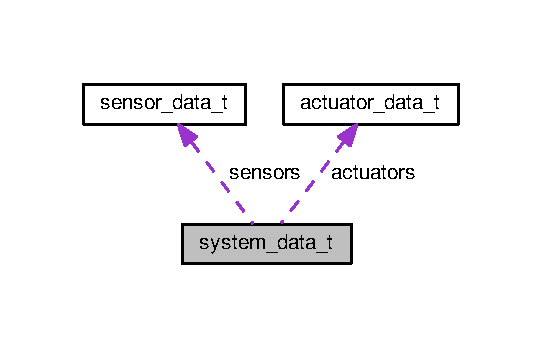
\includegraphics[width=260pt]{structsystem__data__t__coll__graph}
\end{center}
\end{figure}
\subsection*{Public Attributes}
\begin{DoxyCompactItemize}
\item 
int16\+\_\+t \hyperlink{structsystem__data__t_aee87dc3d6b863923bd540334bdaf7198}{wheel\+\_\+speed}
\item 
int16\+\_\+t \hyperlink{structsystem__data__t_a4a161245589e538f2dbf1f888bb06857}{imu\+\_\+angle}
\item 
uint16\+\_\+t \hyperlink{structsystem__data__t_a05ff19dd9bbb2935149dcfa9315f8b6e}{right\+\_\+\+T\+OF}
\item 
uint16\+\_\+t \hyperlink{structsystem__data__t_a664969580339c409aeec2e53c7f7208c}{left\+\_\+\+T\+OF}
\item 
uint16\+\_\+t \hyperlink{structsystem__data__t_a204de6b964d546015c89e985536a74f4}{rear\+\_\+\+T\+OF}
\item 
uint16\+\_\+t \hyperlink{structsystem__data__t_a9fe4bade316d8e0c28fadb24577b146e}{drive\+\_\+mode\+\_\+1}
\item 
uint16\+\_\+t \hyperlink{structsystem__data__t_a26e996fd84c3c87ddac3b2895ea3685e}{drive\+\_\+mode\+\_\+2}
\item 
int16\+\_\+t \hyperlink{structsystem__data__t_a55efc5a76bae9ae7b9b45e13b5eeb994}{motor\+\_\+output}
\item 
int16\+\_\+t \hyperlink{structsystem__data__t_adb14fc1061a46141fc31c93bbe654d1a}{steer\+\_\+output}
\item 
uint16\+\_\+t \hyperlink{structsystem__data__t_a39264c99abb0352fd753848338b550ec}{fifth\+\_\+output}
\item 
bool \hyperlink{structsystem__data__t_a6ea67f53cc727010fd3c19082a42f15f}{updated}
\item 
int16\+\_\+t \hyperlink{structsystem__data__t_acb1f4d615fa9f230fd9a55081b41be53}{deadman}
\item 
int16\+\_\+t \hyperlink{structsystem__data__t_a9fe0717b793ec25c2941eb580540b658}{drive\+\_\+mode}
\item 
\hyperlink{structsensor__data__t}{sensor\+\_\+data\+\_\+t} \hyperlink{structsystem__data__t_a4d59d16a53e21eaba5f9c7212c8d0e63}{sensors}
\item 
\hyperlink{structactuator__data__t}{actuator\+\_\+data\+\_\+t} \hyperlink{structsystem__data__t_a3887ae8b12fbc3ae54b0a89c0f1af1ac}{actuators}
\end{DoxyCompactItemize}


\subsection{Member Data Documentation}
\index{system\+\_\+data\+\_\+t@{system\+\_\+data\+\_\+t}!actuators@{actuators}}
\index{actuators@{actuators}!system\+\_\+data\+\_\+t@{system\+\_\+data\+\_\+t}}
\subsubsection[{\texorpdfstring{actuators}{actuators}}]{\setlength{\rightskip}{0pt plus 5cm}{\bf actuator\+\_\+data\+\_\+t} system\+\_\+data\+\_\+t\+::actuators}\hypertarget{structsystem__data__t_a3887ae8b12fbc3ae54b0a89c0f1af1ac}{}\label{structsystem__data__t_a3887ae8b12fbc3ae54b0a89c0f1af1ac}
\index{system\+\_\+data\+\_\+t@{system\+\_\+data\+\_\+t}!deadman@{deadman}}
\index{deadman@{deadman}!system\+\_\+data\+\_\+t@{system\+\_\+data\+\_\+t}}
\subsubsection[{\texorpdfstring{deadman}{deadman}}]{\setlength{\rightskip}{0pt plus 5cm}int16\+\_\+t system\+\_\+data\+\_\+t\+::deadman}\hypertarget{structsystem__data__t_acb1f4d615fa9f230fd9a55081b41be53}{}\label{structsystem__data__t_acb1f4d615fa9f230fd9a55081b41be53}
\index{system\+\_\+data\+\_\+t@{system\+\_\+data\+\_\+t}!drive\+\_\+mode@{drive\+\_\+mode}}
\index{drive\+\_\+mode@{drive\+\_\+mode}!system\+\_\+data\+\_\+t@{system\+\_\+data\+\_\+t}}
\subsubsection[{\texorpdfstring{drive\+\_\+mode}{drive_mode}}]{\setlength{\rightskip}{0pt plus 5cm}int16\+\_\+t system\+\_\+data\+\_\+t\+::drive\+\_\+mode}\hypertarget{structsystem__data__t_a9fe0717b793ec25c2941eb580540b658}{}\label{structsystem__data__t_a9fe0717b793ec25c2941eb580540b658}
\index{system\+\_\+data\+\_\+t@{system\+\_\+data\+\_\+t}!drive\+\_\+mode\+\_\+1@{drive\+\_\+mode\+\_\+1}}
\index{drive\+\_\+mode\+\_\+1@{drive\+\_\+mode\+\_\+1}!system\+\_\+data\+\_\+t@{system\+\_\+data\+\_\+t}}
\subsubsection[{\texorpdfstring{drive\+\_\+mode\+\_\+1}{drive_mode_1}}]{\setlength{\rightskip}{0pt plus 5cm}uint16\+\_\+t system\+\_\+data\+\_\+t\+::drive\+\_\+mode\+\_\+1}\hypertarget{structsystem__data__t_a9fe4bade316d8e0c28fadb24577b146e}{}\label{structsystem__data__t_a9fe4bade316d8e0c28fadb24577b146e}
\index{system\+\_\+data\+\_\+t@{system\+\_\+data\+\_\+t}!drive\+\_\+mode\+\_\+2@{drive\+\_\+mode\+\_\+2}}
\index{drive\+\_\+mode\+\_\+2@{drive\+\_\+mode\+\_\+2}!system\+\_\+data\+\_\+t@{system\+\_\+data\+\_\+t}}
\subsubsection[{\texorpdfstring{drive\+\_\+mode\+\_\+2}{drive_mode_2}}]{\setlength{\rightskip}{0pt plus 5cm}uint16\+\_\+t system\+\_\+data\+\_\+t\+::drive\+\_\+mode\+\_\+2}\hypertarget{structsystem__data__t_a26e996fd84c3c87ddac3b2895ea3685e}{}\label{structsystem__data__t_a26e996fd84c3c87ddac3b2895ea3685e}
\index{system\+\_\+data\+\_\+t@{system\+\_\+data\+\_\+t}!fifth\+\_\+output@{fifth\+\_\+output}}
\index{fifth\+\_\+output@{fifth\+\_\+output}!system\+\_\+data\+\_\+t@{system\+\_\+data\+\_\+t}}
\subsubsection[{\texorpdfstring{fifth\+\_\+output}{fifth_output}}]{\setlength{\rightskip}{0pt plus 5cm}uint16\+\_\+t system\+\_\+data\+\_\+t\+::fifth\+\_\+output}\hypertarget{structsystem__data__t_a39264c99abb0352fd753848338b550ec}{}\label{structsystem__data__t_a39264c99abb0352fd753848338b550ec}
\index{system\+\_\+data\+\_\+t@{system\+\_\+data\+\_\+t}!imu\+\_\+angle@{imu\+\_\+angle}}
\index{imu\+\_\+angle@{imu\+\_\+angle}!system\+\_\+data\+\_\+t@{system\+\_\+data\+\_\+t}}
\subsubsection[{\texorpdfstring{imu\+\_\+angle}{imu_angle}}]{\setlength{\rightskip}{0pt plus 5cm}int16\+\_\+t system\+\_\+data\+\_\+t\+::imu\+\_\+angle}\hypertarget{structsystem__data__t_a4a161245589e538f2dbf1f888bb06857}{}\label{structsystem__data__t_a4a161245589e538f2dbf1f888bb06857}
\index{system\+\_\+data\+\_\+t@{system\+\_\+data\+\_\+t}!left\+\_\+\+T\+OF@{left\+\_\+\+T\+OF}}
\index{left\+\_\+\+T\+OF@{left\+\_\+\+T\+OF}!system\+\_\+data\+\_\+t@{system\+\_\+data\+\_\+t}}
\subsubsection[{\texorpdfstring{left\+\_\+\+T\+OF}{left_TOF}}]{\setlength{\rightskip}{0pt plus 5cm}uint16\+\_\+t system\+\_\+data\+\_\+t\+::left\+\_\+\+T\+OF}\hypertarget{structsystem__data__t_a664969580339c409aeec2e53c7f7208c}{}\label{structsystem__data__t_a664969580339c409aeec2e53c7f7208c}
\index{system\+\_\+data\+\_\+t@{system\+\_\+data\+\_\+t}!motor\+\_\+output@{motor\+\_\+output}}
\index{motor\+\_\+output@{motor\+\_\+output}!system\+\_\+data\+\_\+t@{system\+\_\+data\+\_\+t}}
\subsubsection[{\texorpdfstring{motor\+\_\+output}{motor_output}}]{\setlength{\rightskip}{0pt plus 5cm}int16\+\_\+t system\+\_\+data\+\_\+t\+::motor\+\_\+output}\hypertarget{structsystem__data__t_a55efc5a76bae9ae7b9b45e13b5eeb994}{}\label{structsystem__data__t_a55efc5a76bae9ae7b9b45e13b5eeb994}
\index{system\+\_\+data\+\_\+t@{system\+\_\+data\+\_\+t}!rear\+\_\+\+T\+OF@{rear\+\_\+\+T\+OF}}
\index{rear\+\_\+\+T\+OF@{rear\+\_\+\+T\+OF}!system\+\_\+data\+\_\+t@{system\+\_\+data\+\_\+t}}
\subsubsection[{\texorpdfstring{rear\+\_\+\+T\+OF}{rear_TOF}}]{\setlength{\rightskip}{0pt plus 5cm}uint16\+\_\+t system\+\_\+data\+\_\+t\+::rear\+\_\+\+T\+OF}\hypertarget{structsystem__data__t_a204de6b964d546015c89e985536a74f4}{}\label{structsystem__data__t_a204de6b964d546015c89e985536a74f4}
\index{system\+\_\+data\+\_\+t@{system\+\_\+data\+\_\+t}!right\+\_\+\+T\+OF@{right\+\_\+\+T\+OF}}
\index{right\+\_\+\+T\+OF@{right\+\_\+\+T\+OF}!system\+\_\+data\+\_\+t@{system\+\_\+data\+\_\+t}}
\subsubsection[{\texorpdfstring{right\+\_\+\+T\+OF}{right_TOF}}]{\setlength{\rightskip}{0pt plus 5cm}uint16\+\_\+t system\+\_\+data\+\_\+t\+::right\+\_\+\+T\+OF}\hypertarget{structsystem__data__t_a05ff19dd9bbb2935149dcfa9315f8b6e}{}\label{structsystem__data__t_a05ff19dd9bbb2935149dcfa9315f8b6e}
\index{system\+\_\+data\+\_\+t@{system\+\_\+data\+\_\+t}!sensors@{sensors}}
\index{sensors@{sensors}!system\+\_\+data\+\_\+t@{system\+\_\+data\+\_\+t}}
\subsubsection[{\texorpdfstring{sensors}{sensors}}]{\setlength{\rightskip}{0pt plus 5cm}{\bf sensor\+\_\+data\+\_\+t} system\+\_\+data\+\_\+t\+::sensors}\hypertarget{structsystem__data__t_a4d59d16a53e21eaba5f9c7212c8d0e63}{}\label{structsystem__data__t_a4d59d16a53e21eaba5f9c7212c8d0e63}
\index{system\+\_\+data\+\_\+t@{system\+\_\+data\+\_\+t}!steer\+\_\+output@{steer\+\_\+output}}
\index{steer\+\_\+output@{steer\+\_\+output}!system\+\_\+data\+\_\+t@{system\+\_\+data\+\_\+t}}
\subsubsection[{\texorpdfstring{steer\+\_\+output}{steer_output}}]{\setlength{\rightskip}{0pt plus 5cm}int16\+\_\+t system\+\_\+data\+\_\+t\+::steer\+\_\+output}\hypertarget{structsystem__data__t_adb14fc1061a46141fc31c93bbe654d1a}{}\label{structsystem__data__t_adb14fc1061a46141fc31c93bbe654d1a}
\index{system\+\_\+data\+\_\+t@{system\+\_\+data\+\_\+t}!updated@{updated}}
\index{updated@{updated}!system\+\_\+data\+\_\+t@{system\+\_\+data\+\_\+t}}
\subsubsection[{\texorpdfstring{updated}{updated}}]{\setlength{\rightskip}{0pt plus 5cm}bool system\+\_\+data\+\_\+t\+::updated}\hypertarget{structsystem__data__t_a6ea67f53cc727010fd3c19082a42f15f}{}\label{structsystem__data__t_a6ea67f53cc727010fd3c19082a42f15f}
\index{system\+\_\+data\+\_\+t@{system\+\_\+data\+\_\+t}!wheel\+\_\+speed@{wheel\+\_\+speed}}
\index{wheel\+\_\+speed@{wheel\+\_\+speed}!system\+\_\+data\+\_\+t@{system\+\_\+data\+\_\+t}}
\subsubsection[{\texorpdfstring{wheel\+\_\+speed}{wheel_speed}}]{\setlength{\rightskip}{0pt plus 5cm}int16\+\_\+t system\+\_\+data\+\_\+t\+::wheel\+\_\+speed}\hypertarget{structsystem__data__t_aee87dc3d6b863923bd540334bdaf7198}{}\label{structsystem__data__t_aee87dc3d6b863923bd540334bdaf7198}


The documentation for this struct was generated from the following file\+:\begin{DoxyCompactItemize}
\item 
daimtronics/semi\+\_\+catkin\+\_\+ws/src/semi\+\_\+truck/include/\hyperlink{semi__catkin__ws_2src_2semi__truck_2include_2system__data_8h}{system\+\_\+data.\+h}\end{DoxyCompactItemize}

\hypertarget{structsemi__truck_1_1_teensy___actuators__}{}\section{semi\+\_\+truck\+:\+:Teensy\+\_\+\+Actuators\+\_\+$<$ Container\+Allocator $>$ Struct Template Reference}
\label{structsemi__truck_1_1_teensy___actuators__}\index{semi\+\_\+truck\+::\+Teensy\+\_\+\+Actuators\+\_\+$<$ Container\+Allocator $>$@{semi\+\_\+truck\+::\+Teensy\+\_\+\+Actuators\+\_\+$<$ Container\+Allocator $>$}}


{\ttfamily \#include $<$Teensy\+\_\+\+Actuators.\+h$>$}

\subsection*{Public Types}
\begin{DoxyCompactItemize}
\item 
typedef \hyperlink{structsemi__truck_1_1_teensy___actuators__}{Teensy\+\_\+\+Actuators\+\_\+}$<$ Container\+Allocator $>$ \hyperlink{structsemi__truck_1_1_teensy___actuators___a56c375933030c0e19bf7694945bd84af}{Type}
\item 
typedef int16\+\_\+t \hyperlink{structsemi__truck_1_1_teensy___actuators___a1cefa1e8e0f45e76b2f6322407c74ab1}{\+\_\+motor\+\_\+output\+\_\+type}
\item 
typedef int16\+\_\+t \hyperlink{structsemi__truck_1_1_teensy___actuators___a38b3265a1e0521620575f2cdcec23d1a}{\+\_\+steer\+\_\+output\+\_\+type}
\item 
typedef int16\+\_\+t \hyperlink{structsemi__truck_1_1_teensy___actuators___ac866dd52df9dc5d61aac2c073d49c91b}{\+\_\+fifth\+\_\+output\+\_\+type}
\item 
typedef boost\+::shared\+\_\+ptr$<$ \+::\hyperlink{structsemi__truck_1_1_teensy___actuators__}{semi\+\_\+truck\+::\+Teensy\+\_\+\+Actuators\+\_\+}$<$ Container\+Allocator $>$ $>$ \hyperlink{structsemi__truck_1_1_teensy___actuators___a5146b132d18f66dab87b575f3591049f}{Ptr}
\item 
typedef boost\+::shared\+\_\+ptr$<$ \+::\hyperlink{structsemi__truck_1_1_teensy___actuators__}{semi\+\_\+truck\+::\+Teensy\+\_\+\+Actuators\+\_\+}$<$ Container\+Allocator $>$ const  $>$ \hyperlink{structsemi__truck_1_1_teensy___actuators___a7a0d58ea72ee326dfe3e3476ae6ef61f}{Const\+Ptr}
\end{DoxyCompactItemize}
\subsection*{Public Member Functions}
\begin{DoxyCompactItemize}
\item 
\hyperlink{structsemi__truck_1_1_teensy___actuators___ad09b32ec959790bca4f07de7d79f138e}{Teensy\+\_\+\+Actuators\+\_\+} ()
\item 
\hyperlink{structsemi__truck_1_1_teensy___actuators___a61de3eb36f071a8067fb7e0d86cbc3e6}{Teensy\+\_\+\+Actuators\+\_\+} (const Container\+Allocator \&\+\_\+alloc)
\end{DoxyCompactItemize}
\subsection*{Public Attributes}
\begin{DoxyCompactItemize}
\item 
\hyperlink{structsemi__truck_1_1_teensy___actuators___a1cefa1e8e0f45e76b2f6322407c74ab1}{\+\_\+motor\+\_\+output\+\_\+type} \hyperlink{structsemi__truck_1_1_teensy___actuators___a9157e40c9500ca6bbd20f4938dcb5a9b}{motor\+\_\+output}
\item 
\hyperlink{structsemi__truck_1_1_teensy___actuators___a38b3265a1e0521620575f2cdcec23d1a}{\+\_\+steer\+\_\+output\+\_\+type} \hyperlink{structsemi__truck_1_1_teensy___actuators___aa98f0b646061a5b36b71922a6fe0630f}{steer\+\_\+output}
\item 
\hyperlink{structsemi__truck_1_1_teensy___actuators___ac866dd52df9dc5d61aac2c073d49c91b}{\+\_\+fifth\+\_\+output\+\_\+type} \hyperlink{structsemi__truck_1_1_teensy___actuators___ab32dfbbdaec1341c59b86d39e26e4eda}{fifth\+\_\+output}
\end{DoxyCompactItemize}


\subsection{Member Typedef Documentation}
\index{semi\+\_\+truck\+::\+Teensy\+\_\+\+Actuators\+\_\+@{semi\+\_\+truck\+::\+Teensy\+\_\+\+Actuators\+\_\+}!\+\_\+fifth\+\_\+output\+\_\+type@{\+\_\+fifth\+\_\+output\+\_\+type}}
\index{\+\_\+fifth\+\_\+output\+\_\+type@{\+\_\+fifth\+\_\+output\+\_\+type}!semi\+\_\+truck\+::\+Teensy\+\_\+\+Actuators\+\_\+@{semi\+\_\+truck\+::\+Teensy\+\_\+\+Actuators\+\_\+}}
\subsubsection[{\texorpdfstring{\+\_\+fifth\+\_\+output\+\_\+type}{_fifth_output_type}}]{\setlength{\rightskip}{0pt plus 5cm}template$<$class Container\+Allocator $>$ typedef int16\+\_\+t {\bf semi\+\_\+truck\+::\+Teensy\+\_\+\+Actuators\+\_\+}$<$ Container\+Allocator $>$\+::{\bf \+\_\+fifth\+\_\+output\+\_\+type}}\hypertarget{structsemi__truck_1_1_teensy___actuators___ac866dd52df9dc5d61aac2c073d49c91b}{}\label{structsemi__truck_1_1_teensy___actuators___ac866dd52df9dc5d61aac2c073d49c91b}
\index{semi\+\_\+truck\+::\+Teensy\+\_\+\+Actuators\+\_\+@{semi\+\_\+truck\+::\+Teensy\+\_\+\+Actuators\+\_\+}!\+\_\+motor\+\_\+output\+\_\+type@{\+\_\+motor\+\_\+output\+\_\+type}}
\index{\+\_\+motor\+\_\+output\+\_\+type@{\+\_\+motor\+\_\+output\+\_\+type}!semi\+\_\+truck\+::\+Teensy\+\_\+\+Actuators\+\_\+@{semi\+\_\+truck\+::\+Teensy\+\_\+\+Actuators\+\_\+}}
\subsubsection[{\texorpdfstring{\+\_\+motor\+\_\+output\+\_\+type}{_motor_output_type}}]{\setlength{\rightskip}{0pt plus 5cm}template$<$class Container\+Allocator $>$ typedef int16\+\_\+t {\bf semi\+\_\+truck\+::\+Teensy\+\_\+\+Actuators\+\_\+}$<$ Container\+Allocator $>$\+::{\bf \+\_\+motor\+\_\+output\+\_\+type}}\hypertarget{structsemi__truck_1_1_teensy___actuators___a1cefa1e8e0f45e76b2f6322407c74ab1}{}\label{structsemi__truck_1_1_teensy___actuators___a1cefa1e8e0f45e76b2f6322407c74ab1}
\index{semi\+\_\+truck\+::\+Teensy\+\_\+\+Actuators\+\_\+@{semi\+\_\+truck\+::\+Teensy\+\_\+\+Actuators\+\_\+}!\+\_\+steer\+\_\+output\+\_\+type@{\+\_\+steer\+\_\+output\+\_\+type}}
\index{\+\_\+steer\+\_\+output\+\_\+type@{\+\_\+steer\+\_\+output\+\_\+type}!semi\+\_\+truck\+::\+Teensy\+\_\+\+Actuators\+\_\+@{semi\+\_\+truck\+::\+Teensy\+\_\+\+Actuators\+\_\+}}
\subsubsection[{\texorpdfstring{\+\_\+steer\+\_\+output\+\_\+type}{_steer_output_type}}]{\setlength{\rightskip}{0pt plus 5cm}template$<$class Container\+Allocator $>$ typedef int16\+\_\+t {\bf semi\+\_\+truck\+::\+Teensy\+\_\+\+Actuators\+\_\+}$<$ Container\+Allocator $>$\+::{\bf \+\_\+steer\+\_\+output\+\_\+type}}\hypertarget{structsemi__truck_1_1_teensy___actuators___a38b3265a1e0521620575f2cdcec23d1a}{}\label{structsemi__truck_1_1_teensy___actuators___a38b3265a1e0521620575f2cdcec23d1a}
\index{semi\+\_\+truck\+::\+Teensy\+\_\+\+Actuators\+\_\+@{semi\+\_\+truck\+::\+Teensy\+\_\+\+Actuators\+\_\+}!Const\+Ptr@{Const\+Ptr}}
\index{Const\+Ptr@{Const\+Ptr}!semi\+\_\+truck\+::\+Teensy\+\_\+\+Actuators\+\_\+@{semi\+\_\+truck\+::\+Teensy\+\_\+\+Actuators\+\_\+}}
\subsubsection[{\texorpdfstring{Const\+Ptr}{ConstPtr}}]{\setlength{\rightskip}{0pt plus 5cm}template$<$class Container\+Allocator $>$ typedef boost\+::shared\+\_\+ptr$<$ \+::{\bf semi\+\_\+truck\+::\+Teensy\+\_\+\+Actuators\+\_\+}$<$Container\+Allocator$>$ const$>$ {\bf semi\+\_\+truck\+::\+Teensy\+\_\+\+Actuators\+\_\+}$<$ Container\+Allocator $>$\+::{\bf Const\+Ptr}}\hypertarget{structsemi__truck_1_1_teensy___actuators___a7a0d58ea72ee326dfe3e3476ae6ef61f}{}\label{structsemi__truck_1_1_teensy___actuators___a7a0d58ea72ee326dfe3e3476ae6ef61f}
\index{semi\+\_\+truck\+::\+Teensy\+\_\+\+Actuators\+\_\+@{semi\+\_\+truck\+::\+Teensy\+\_\+\+Actuators\+\_\+}!Ptr@{Ptr}}
\index{Ptr@{Ptr}!semi\+\_\+truck\+::\+Teensy\+\_\+\+Actuators\+\_\+@{semi\+\_\+truck\+::\+Teensy\+\_\+\+Actuators\+\_\+}}
\subsubsection[{\texorpdfstring{Ptr}{Ptr}}]{\setlength{\rightskip}{0pt plus 5cm}template$<$class Container\+Allocator $>$ typedef boost\+::shared\+\_\+ptr$<$ \+::{\bf semi\+\_\+truck\+::\+Teensy\+\_\+\+Actuators\+\_\+}$<$Container\+Allocator$>$ $>$ {\bf semi\+\_\+truck\+::\+Teensy\+\_\+\+Actuators\+\_\+}$<$ Container\+Allocator $>$\+::{\bf Ptr}}\hypertarget{structsemi__truck_1_1_teensy___actuators___a5146b132d18f66dab87b575f3591049f}{}\label{structsemi__truck_1_1_teensy___actuators___a5146b132d18f66dab87b575f3591049f}
\index{semi\+\_\+truck\+::\+Teensy\+\_\+\+Actuators\+\_\+@{semi\+\_\+truck\+::\+Teensy\+\_\+\+Actuators\+\_\+}!Type@{Type}}
\index{Type@{Type}!semi\+\_\+truck\+::\+Teensy\+\_\+\+Actuators\+\_\+@{semi\+\_\+truck\+::\+Teensy\+\_\+\+Actuators\+\_\+}}
\subsubsection[{\texorpdfstring{Type}{Type}}]{\setlength{\rightskip}{0pt plus 5cm}template$<$class Container\+Allocator $>$ typedef {\bf Teensy\+\_\+\+Actuators\+\_\+}$<$Container\+Allocator$>$ {\bf semi\+\_\+truck\+::\+Teensy\+\_\+\+Actuators\+\_\+}$<$ Container\+Allocator $>$\+::{\bf Type}}\hypertarget{structsemi__truck_1_1_teensy___actuators___a56c375933030c0e19bf7694945bd84af}{}\label{structsemi__truck_1_1_teensy___actuators___a56c375933030c0e19bf7694945bd84af}


\subsection{Constructor \& Destructor Documentation}
\index{semi\+\_\+truck\+::\+Teensy\+\_\+\+Actuators\+\_\+@{semi\+\_\+truck\+::\+Teensy\+\_\+\+Actuators\+\_\+}!Teensy\+\_\+\+Actuators\+\_\+@{Teensy\+\_\+\+Actuators\+\_\+}}
\index{Teensy\+\_\+\+Actuators\+\_\+@{Teensy\+\_\+\+Actuators\+\_\+}!semi\+\_\+truck\+::\+Teensy\+\_\+\+Actuators\+\_\+@{semi\+\_\+truck\+::\+Teensy\+\_\+\+Actuators\+\_\+}}
\subsubsection[{\texorpdfstring{Teensy\+\_\+\+Actuators\+\_\+()}{Teensy_Actuators_()}}]{\setlength{\rightskip}{0pt plus 5cm}template$<$class Container\+Allocator $>$ {\bf semi\+\_\+truck\+::\+Teensy\+\_\+\+Actuators\+\_\+}$<$ Container\+Allocator $>$\+::{\bf Teensy\+\_\+\+Actuators\+\_\+} (
\begin{DoxyParamCaption}
{}
\end{DoxyParamCaption}
)\hspace{0.3cm}{\ttfamily [inline]}}\hypertarget{structsemi__truck_1_1_teensy___actuators___ad09b32ec959790bca4f07de7d79f138e}{}\label{structsemi__truck_1_1_teensy___actuators___ad09b32ec959790bca4f07de7d79f138e}
\index{semi\+\_\+truck\+::\+Teensy\+\_\+\+Actuators\+\_\+@{semi\+\_\+truck\+::\+Teensy\+\_\+\+Actuators\+\_\+}!Teensy\+\_\+\+Actuators\+\_\+@{Teensy\+\_\+\+Actuators\+\_\+}}
\index{Teensy\+\_\+\+Actuators\+\_\+@{Teensy\+\_\+\+Actuators\+\_\+}!semi\+\_\+truck\+::\+Teensy\+\_\+\+Actuators\+\_\+@{semi\+\_\+truck\+::\+Teensy\+\_\+\+Actuators\+\_\+}}
\subsubsection[{\texorpdfstring{Teensy\+\_\+\+Actuators\+\_\+(const Container\+Allocator \&\+\_\+alloc)}{Teensy_Actuators_(const ContainerAllocator &_alloc)}}]{\setlength{\rightskip}{0pt plus 5cm}template$<$class Container\+Allocator $>$ {\bf semi\+\_\+truck\+::\+Teensy\+\_\+\+Actuators\+\_\+}$<$ Container\+Allocator $>$\+::{\bf Teensy\+\_\+\+Actuators\+\_\+} (
\begin{DoxyParamCaption}
\item[{const Container\+Allocator \&}]{\+\_\+alloc}
\end{DoxyParamCaption}
)\hspace{0.3cm}{\ttfamily [inline]}}\hypertarget{structsemi__truck_1_1_teensy___actuators___a61de3eb36f071a8067fb7e0d86cbc3e6}{}\label{structsemi__truck_1_1_teensy___actuators___a61de3eb36f071a8067fb7e0d86cbc3e6}


\subsection{Member Data Documentation}
\index{semi\+\_\+truck\+::\+Teensy\+\_\+\+Actuators\+\_\+@{semi\+\_\+truck\+::\+Teensy\+\_\+\+Actuators\+\_\+}!fifth\+\_\+output@{fifth\+\_\+output}}
\index{fifth\+\_\+output@{fifth\+\_\+output}!semi\+\_\+truck\+::\+Teensy\+\_\+\+Actuators\+\_\+@{semi\+\_\+truck\+::\+Teensy\+\_\+\+Actuators\+\_\+}}
\subsubsection[{\texorpdfstring{fifth\+\_\+output}{fifth_output}}]{\setlength{\rightskip}{0pt plus 5cm}template$<$class Container\+Allocator $>$ {\bf \+\_\+fifth\+\_\+output\+\_\+type} {\bf semi\+\_\+truck\+::\+Teensy\+\_\+\+Actuators\+\_\+}$<$ Container\+Allocator $>$\+::fifth\+\_\+output}\hypertarget{structsemi__truck_1_1_teensy___actuators___ab32dfbbdaec1341c59b86d39e26e4eda}{}\label{structsemi__truck_1_1_teensy___actuators___ab32dfbbdaec1341c59b86d39e26e4eda}
\index{semi\+\_\+truck\+::\+Teensy\+\_\+\+Actuators\+\_\+@{semi\+\_\+truck\+::\+Teensy\+\_\+\+Actuators\+\_\+}!motor\+\_\+output@{motor\+\_\+output}}
\index{motor\+\_\+output@{motor\+\_\+output}!semi\+\_\+truck\+::\+Teensy\+\_\+\+Actuators\+\_\+@{semi\+\_\+truck\+::\+Teensy\+\_\+\+Actuators\+\_\+}}
\subsubsection[{\texorpdfstring{motor\+\_\+output}{motor_output}}]{\setlength{\rightskip}{0pt plus 5cm}template$<$class Container\+Allocator $>$ {\bf \+\_\+motor\+\_\+output\+\_\+type} {\bf semi\+\_\+truck\+::\+Teensy\+\_\+\+Actuators\+\_\+}$<$ Container\+Allocator $>$\+::motor\+\_\+output}\hypertarget{structsemi__truck_1_1_teensy___actuators___a9157e40c9500ca6bbd20f4938dcb5a9b}{}\label{structsemi__truck_1_1_teensy___actuators___a9157e40c9500ca6bbd20f4938dcb5a9b}
\index{semi\+\_\+truck\+::\+Teensy\+\_\+\+Actuators\+\_\+@{semi\+\_\+truck\+::\+Teensy\+\_\+\+Actuators\+\_\+}!steer\+\_\+output@{steer\+\_\+output}}
\index{steer\+\_\+output@{steer\+\_\+output}!semi\+\_\+truck\+::\+Teensy\+\_\+\+Actuators\+\_\+@{semi\+\_\+truck\+::\+Teensy\+\_\+\+Actuators\+\_\+}}
\subsubsection[{\texorpdfstring{steer\+\_\+output}{steer_output}}]{\setlength{\rightskip}{0pt plus 5cm}template$<$class Container\+Allocator $>$ {\bf \+\_\+steer\+\_\+output\+\_\+type} {\bf semi\+\_\+truck\+::\+Teensy\+\_\+\+Actuators\+\_\+}$<$ Container\+Allocator $>$\+::steer\+\_\+output}\hypertarget{structsemi__truck_1_1_teensy___actuators___aa98f0b646061a5b36b71922a6fe0630f}{}\label{structsemi__truck_1_1_teensy___actuators___aa98f0b646061a5b36b71922a6fe0630f}


The documentation for this struct was generated from the following file\+:\begin{DoxyCompactItemize}
\item 
daimtronics/semi\+\_\+catkin\+\_\+ws/src/semi\+\_\+truck/include/\hyperlink{_teensy___actuators_8h}{Teensy\+\_\+\+Actuators.\+h}\end{DoxyCompactItemize}

\hypertarget{structsemi__truck_1_1_teensy___sensors__}{}\section{semi\+\_\+truck\+:\+:Teensy\+\_\+\+Sensors\+\_\+$<$ Container\+Allocator $>$ Struct Template Reference}
\label{structsemi__truck_1_1_teensy___sensors__}\index{semi\+\_\+truck\+::\+Teensy\+\_\+\+Sensors\+\_\+$<$ Container\+Allocator $>$@{semi\+\_\+truck\+::\+Teensy\+\_\+\+Sensors\+\_\+$<$ Container\+Allocator $>$}}


{\ttfamily \#include $<$Teensy\+\_\+\+Sensors.\+h$>$}

\subsection*{Public Types}
\begin{DoxyCompactItemize}
\item 
typedef \hyperlink{structsemi__truck_1_1_teensy___sensors__}{Teensy\+\_\+\+Sensors\+\_\+}$<$ Container\+Allocator $>$ \hyperlink{structsemi__truck_1_1_teensy___sensors___a05a02769de72554dbc9d24a583752523}{Type}
\item 
typedef int16\+\_\+t \hyperlink{structsemi__truck_1_1_teensy___sensors___adca9245fde7f0f8121fed20243c9ae1a}{\+\_\+wheel\+\_\+speed\+\_\+type}
\item 
typedef int16\+\_\+t \hyperlink{structsemi__truck_1_1_teensy___sensors___aaf882f7b6732e41e25877c88eb8a1c7a}{\+\_\+imu\+\_\+angle\+\_\+type}
\item 
typedef int16\+\_\+t \hyperlink{structsemi__truck_1_1_teensy___sensors___adb98ef7b91b8a2c8346a2b36e1816a61}{\+\_\+right\+\_\+\+T\+O\+F\+\_\+type}
\item 
typedef int16\+\_\+t \hyperlink{structsemi__truck_1_1_teensy___sensors___ad6ac104c65141acb58bf4af051941136}{\+\_\+left\+\_\+\+T\+O\+F\+\_\+type}
\item 
typedef int16\+\_\+t \hyperlink{structsemi__truck_1_1_teensy___sensors___ab8ba6b899ad8e9de101aa904e646d7e9}{\+\_\+rear\+\_\+\+T\+O\+F\+\_\+type}
\item 
typedef int16\+\_\+t \hyperlink{structsemi__truck_1_1_teensy___sensors___afd1593af87fe24f82e4cdc3db0695f0d}{\+\_\+drive\+\_\+mode\+\_\+1\+\_\+type}
\item 
typedef int16\+\_\+t \hyperlink{structsemi__truck_1_1_teensy___sensors___aca8d2a953d712ec418fb0d13877b7194}{\+\_\+drive\+\_\+mode\+\_\+2\+\_\+type}
\item 
typedef boost\+::shared\+\_\+ptr$<$ \+::\hyperlink{structsemi__truck_1_1_teensy___sensors__}{semi\+\_\+truck\+::\+Teensy\+\_\+\+Sensors\+\_\+}$<$ Container\+Allocator $>$ $>$ \hyperlink{structsemi__truck_1_1_teensy___sensors___a31b2377d32f460ee7ebdcfe467f70b12}{Ptr}
\item 
typedef boost\+::shared\+\_\+ptr$<$ \+::\hyperlink{structsemi__truck_1_1_teensy___sensors__}{semi\+\_\+truck\+::\+Teensy\+\_\+\+Sensors\+\_\+}$<$ Container\+Allocator $>$ const  $>$ \hyperlink{structsemi__truck_1_1_teensy___sensors___a1c67c299fc5270cf253a6e5fbafe9ce8}{Const\+Ptr}
\end{DoxyCompactItemize}
\subsection*{Public Member Functions}
\begin{DoxyCompactItemize}
\item 
\hyperlink{structsemi__truck_1_1_teensy___sensors___a6c5e97f6398548c5bdaebcba271a3e45}{Teensy\+\_\+\+Sensors\+\_\+} ()
\item 
\hyperlink{structsemi__truck_1_1_teensy___sensors___a629bceff34222229769c25ed8f074531}{Teensy\+\_\+\+Sensors\+\_\+} (const Container\+Allocator \&\+\_\+alloc)
\end{DoxyCompactItemize}
\subsection*{Public Attributes}
\begin{DoxyCompactItemize}
\item 
\hyperlink{structsemi__truck_1_1_teensy___sensors___adca9245fde7f0f8121fed20243c9ae1a}{\+\_\+wheel\+\_\+speed\+\_\+type} \hyperlink{structsemi__truck_1_1_teensy___sensors___adbe8f5f099fb3077164702fc3af3c739}{wheel\+\_\+speed}
\item 
\hyperlink{structsemi__truck_1_1_teensy___sensors___aaf882f7b6732e41e25877c88eb8a1c7a}{\+\_\+imu\+\_\+angle\+\_\+type} \hyperlink{structsemi__truck_1_1_teensy___sensors___a329db78dcc3e9b42a390c48fdf99784e}{imu\+\_\+angle}
\item 
\hyperlink{structsemi__truck_1_1_teensy___sensors___adb98ef7b91b8a2c8346a2b36e1816a61}{\+\_\+right\+\_\+\+T\+O\+F\+\_\+type} \hyperlink{structsemi__truck_1_1_teensy___sensors___acd1bf8a8cdb1073974200b6ae0c7a179}{right\+\_\+\+T\+OF}
\item 
\hyperlink{structsemi__truck_1_1_teensy___sensors___ad6ac104c65141acb58bf4af051941136}{\+\_\+left\+\_\+\+T\+O\+F\+\_\+type} \hyperlink{structsemi__truck_1_1_teensy___sensors___a202e466979b2978e09428a512337433f}{left\+\_\+\+T\+OF}
\item 
\hyperlink{structsemi__truck_1_1_teensy___sensors___ab8ba6b899ad8e9de101aa904e646d7e9}{\+\_\+rear\+\_\+\+T\+O\+F\+\_\+type} \hyperlink{structsemi__truck_1_1_teensy___sensors___aaed96e5feb07aa8a729524f2b643a4c9}{rear\+\_\+\+T\+OF}
\item 
\hyperlink{structsemi__truck_1_1_teensy___sensors___afd1593af87fe24f82e4cdc3db0695f0d}{\+\_\+drive\+\_\+mode\+\_\+1\+\_\+type} \hyperlink{structsemi__truck_1_1_teensy___sensors___a66b7de9953916baf991d662f58b6d24d}{drive\+\_\+mode\+\_\+1}
\item 
\hyperlink{structsemi__truck_1_1_teensy___sensors___aca8d2a953d712ec418fb0d13877b7194}{\+\_\+drive\+\_\+mode\+\_\+2\+\_\+type} \hyperlink{structsemi__truck_1_1_teensy___sensors___a199ab1bba03a7b86615cc5a5aa197557}{drive\+\_\+mode\+\_\+2}
\end{DoxyCompactItemize}


\subsection{Member Typedef Documentation}
\index{semi\+\_\+truck\+::\+Teensy\+\_\+\+Sensors\+\_\+@{semi\+\_\+truck\+::\+Teensy\+\_\+\+Sensors\+\_\+}!\+\_\+drive\+\_\+mode\+\_\+1\+\_\+type@{\+\_\+drive\+\_\+mode\+\_\+1\+\_\+type}}
\index{\+\_\+drive\+\_\+mode\+\_\+1\+\_\+type@{\+\_\+drive\+\_\+mode\+\_\+1\+\_\+type}!semi\+\_\+truck\+::\+Teensy\+\_\+\+Sensors\+\_\+@{semi\+\_\+truck\+::\+Teensy\+\_\+\+Sensors\+\_\+}}
\subsubsection[{\texorpdfstring{\+\_\+drive\+\_\+mode\+\_\+1\+\_\+type}{_drive_mode_1_type}}]{\setlength{\rightskip}{0pt plus 5cm}template$<$class Container\+Allocator $>$ typedef int16\+\_\+t {\bf semi\+\_\+truck\+::\+Teensy\+\_\+\+Sensors\+\_\+}$<$ Container\+Allocator $>$\+::{\bf \+\_\+drive\+\_\+mode\+\_\+1\+\_\+type}}\hypertarget{structsemi__truck_1_1_teensy___sensors___afd1593af87fe24f82e4cdc3db0695f0d}{}\label{structsemi__truck_1_1_teensy___sensors___afd1593af87fe24f82e4cdc3db0695f0d}
\index{semi\+\_\+truck\+::\+Teensy\+\_\+\+Sensors\+\_\+@{semi\+\_\+truck\+::\+Teensy\+\_\+\+Sensors\+\_\+}!\+\_\+drive\+\_\+mode\+\_\+2\+\_\+type@{\+\_\+drive\+\_\+mode\+\_\+2\+\_\+type}}
\index{\+\_\+drive\+\_\+mode\+\_\+2\+\_\+type@{\+\_\+drive\+\_\+mode\+\_\+2\+\_\+type}!semi\+\_\+truck\+::\+Teensy\+\_\+\+Sensors\+\_\+@{semi\+\_\+truck\+::\+Teensy\+\_\+\+Sensors\+\_\+}}
\subsubsection[{\texorpdfstring{\+\_\+drive\+\_\+mode\+\_\+2\+\_\+type}{_drive_mode_2_type}}]{\setlength{\rightskip}{0pt plus 5cm}template$<$class Container\+Allocator $>$ typedef int16\+\_\+t {\bf semi\+\_\+truck\+::\+Teensy\+\_\+\+Sensors\+\_\+}$<$ Container\+Allocator $>$\+::{\bf \+\_\+drive\+\_\+mode\+\_\+2\+\_\+type}}\hypertarget{structsemi__truck_1_1_teensy___sensors___aca8d2a953d712ec418fb0d13877b7194}{}\label{structsemi__truck_1_1_teensy___sensors___aca8d2a953d712ec418fb0d13877b7194}
\index{semi\+\_\+truck\+::\+Teensy\+\_\+\+Sensors\+\_\+@{semi\+\_\+truck\+::\+Teensy\+\_\+\+Sensors\+\_\+}!\+\_\+imu\+\_\+angle\+\_\+type@{\+\_\+imu\+\_\+angle\+\_\+type}}
\index{\+\_\+imu\+\_\+angle\+\_\+type@{\+\_\+imu\+\_\+angle\+\_\+type}!semi\+\_\+truck\+::\+Teensy\+\_\+\+Sensors\+\_\+@{semi\+\_\+truck\+::\+Teensy\+\_\+\+Sensors\+\_\+}}
\subsubsection[{\texorpdfstring{\+\_\+imu\+\_\+angle\+\_\+type}{_imu_angle_type}}]{\setlength{\rightskip}{0pt plus 5cm}template$<$class Container\+Allocator $>$ typedef int16\+\_\+t {\bf semi\+\_\+truck\+::\+Teensy\+\_\+\+Sensors\+\_\+}$<$ Container\+Allocator $>$\+::{\bf \+\_\+imu\+\_\+angle\+\_\+type}}\hypertarget{structsemi__truck_1_1_teensy___sensors___aaf882f7b6732e41e25877c88eb8a1c7a}{}\label{structsemi__truck_1_1_teensy___sensors___aaf882f7b6732e41e25877c88eb8a1c7a}
\index{semi\+\_\+truck\+::\+Teensy\+\_\+\+Sensors\+\_\+@{semi\+\_\+truck\+::\+Teensy\+\_\+\+Sensors\+\_\+}!\+\_\+left\+\_\+\+T\+O\+F\+\_\+type@{\+\_\+left\+\_\+\+T\+O\+F\+\_\+type}}
\index{\+\_\+left\+\_\+\+T\+O\+F\+\_\+type@{\+\_\+left\+\_\+\+T\+O\+F\+\_\+type}!semi\+\_\+truck\+::\+Teensy\+\_\+\+Sensors\+\_\+@{semi\+\_\+truck\+::\+Teensy\+\_\+\+Sensors\+\_\+}}
\subsubsection[{\texorpdfstring{\+\_\+left\+\_\+\+T\+O\+F\+\_\+type}{_left_TOF_type}}]{\setlength{\rightskip}{0pt plus 5cm}template$<$class Container\+Allocator $>$ typedef int16\+\_\+t {\bf semi\+\_\+truck\+::\+Teensy\+\_\+\+Sensors\+\_\+}$<$ Container\+Allocator $>$\+::{\bf \+\_\+left\+\_\+\+T\+O\+F\+\_\+type}}\hypertarget{structsemi__truck_1_1_teensy___sensors___ad6ac104c65141acb58bf4af051941136}{}\label{structsemi__truck_1_1_teensy___sensors___ad6ac104c65141acb58bf4af051941136}
\index{semi\+\_\+truck\+::\+Teensy\+\_\+\+Sensors\+\_\+@{semi\+\_\+truck\+::\+Teensy\+\_\+\+Sensors\+\_\+}!\+\_\+rear\+\_\+\+T\+O\+F\+\_\+type@{\+\_\+rear\+\_\+\+T\+O\+F\+\_\+type}}
\index{\+\_\+rear\+\_\+\+T\+O\+F\+\_\+type@{\+\_\+rear\+\_\+\+T\+O\+F\+\_\+type}!semi\+\_\+truck\+::\+Teensy\+\_\+\+Sensors\+\_\+@{semi\+\_\+truck\+::\+Teensy\+\_\+\+Sensors\+\_\+}}
\subsubsection[{\texorpdfstring{\+\_\+rear\+\_\+\+T\+O\+F\+\_\+type}{_rear_TOF_type}}]{\setlength{\rightskip}{0pt plus 5cm}template$<$class Container\+Allocator $>$ typedef int16\+\_\+t {\bf semi\+\_\+truck\+::\+Teensy\+\_\+\+Sensors\+\_\+}$<$ Container\+Allocator $>$\+::{\bf \+\_\+rear\+\_\+\+T\+O\+F\+\_\+type}}\hypertarget{structsemi__truck_1_1_teensy___sensors___ab8ba6b899ad8e9de101aa904e646d7e9}{}\label{structsemi__truck_1_1_teensy___sensors___ab8ba6b899ad8e9de101aa904e646d7e9}
\index{semi\+\_\+truck\+::\+Teensy\+\_\+\+Sensors\+\_\+@{semi\+\_\+truck\+::\+Teensy\+\_\+\+Sensors\+\_\+}!\+\_\+right\+\_\+\+T\+O\+F\+\_\+type@{\+\_\+right\+\_\+\+T\+O\+F\+\_\+type}}
\index{\+\_\+right\+\_\+\+T\+O\+F\+\_\+type@{\+\_\+right\+\_\+\+T\+O\+F\+\_\+type}!semi\+\_\+truck\+::\+Teensy\+\_\+\+Sensors\+\_\+@{semi\+\_\+truck\+::\+Teensy\+\_\+\+Sensors\+\_\+}}
\subsubsection[{\texorpdfstring{\+\_\+right\+\_\+\+T\+O\+F\+\_\+type}{_right_TOF_type}}]{\setlength{\rightskip}{0pt plus 5cm}template$<$class Container\+Allocator $>$ typedef int16\+\_\+t {\bf semi\+\_\+truck\+::\+Teensy\+\_\+\+Sensors\+\_\+}$<$ Container\+Allocator $>$\+::{\bf \+\_\+right\+\_\+\+T\+O\+F\+\_\+type}}\hypertarget{structsemi__truck_1_1_teensy___sensors___adb98ef7b91b8a2c8346a2b36e1816a61}{}\label{structsemi__truck_1_1_teensy___sensors___adb98ef7b91b8a2c8346a2b36e1816a61}
\index{semi\+\_\+truck\+::\+Teensy\+\_\+\+Sensors\+\_\+@{semi\+\_\+truck\+::\+Teensy\+\_\+\+Sensors\+\_\+}!\+\_\+wheel\+\_\+speed\+\_\+type@{\+\_\+wheel\+\_\+speed\+\_\+type}}
\index{\+\_\+wheel\+\_\+speed\+\_\+type@{\+\_\+wheel\+\_\+speed\+\_\+type}!semi\+\_\+truck\+::\+Teensy\+\_\+\+Sensors\+\_\+@{semi\+\_\+truck\+::\+Teensy\+\_\+\+Sensors\+\_\+}}
\subsubsection[{\texorpdfstring{\+\_\+wheel\+\_\+speed\+\_\+type}{_wheel_speed_type}}]{\setlength{\rightskip}{0pt plus 5cm}template$<$class Container\+Allocator $>$ typedef int16\+\_\+t {\bf semi\+\_\+truck\+::\+Teensy\+\_\+\+Sensors\+\_\+}$<$ Container\+Allocator $>$\+::{\bf \+\_\+wheel\+\_\+speed\+\_\+type}}\hypertarget{structsemi__truck_1_1_teensy___sensors___adca9245fde7f0f8121fed20243c9ae1a}{}\label{structsemi__truck_1_1_teensy___sensors___adca9245fde7f0f8121fed20243c9ae1a}
\index{semi\+\_\+truck\+::\+Teensy\+\_\+\+Sensors\+\_\+@{semi\+\_\+truck\+::\+Teensy\+\_\+\+Sensors\+\_\+}!Const\+Ptr@{Const\+Ptr}}
\index{Const\+Ptr@{Const\+Ptr}!semi\+\_\+truck\+::\+Teensy\+\_\+\+Sensors\+\_\+@{semi\+\_\+truck\+::\+Teensy\+\_\+\+Sensors\+\_\+}}
\subsubsection[{\texorpdfstring{Const\+Ptr}{ConstPtr}}]{\setlength{\rightskip}{0pt plus 5cm}template$<$class Container\+Allocator $>$ typedef boost\+::shared\+\_\+ptr$<$ \+::{\bf semi\+\_\+truck\+::\+Teensy\+\_\+\+Sensors\+\_\+}$<$Container\+Allocator$>$ const$>$ {\bf semi\+\_\+truck\+::\+Teensy\+\_\+\+Sensors\+\_\+}$<$ Container\+Allocator $>$\+::{\bf Const\+Ptr}}\hypertarget{structsemi__truck_1_1_teensy___sensors___a1c67c299fc5270cf253a6e5fbafe9ce8}{}\label{structsemi__truck_1_1_teensy___sensors___a1c67c299fc5270cf253a6e5fbafe9ce8}
\index{semi\+\_\+truck\+::\+Teensy\+\_\+\+Sensors\+\_\+@{semi\+\_\+truck\+::\+Teensy\+\_\+\+Sensors\+\_\+}!Ptr@{Ptr}}
\index{Ptr@{Ptr}!semi\+\_\+truck\+::\+Teensy\+\_\+\+Sensors\+\_\+@{semi\+\_\+truck\+::\+Teensy\+\_\+\+Sensors\+\_\+}}
\subsubsection[{\texorpdfstring{Ptr}{Ptr}}]{\setlength{\rightskip}{0pt plus 5cm}template$<$class Container\+Allocator $>$ typedef boost\+::shared\+\_\+ptr$<$ \+::{\bf semi\+\_\+truck\+::\+Teensy\+\_\+\+Sensors\+\_\+}$<$Container\+Allocator$>$ $>$ {\bf semi\+\_\+truck\+::\+Teensy\+\_\+\+Sensors\+\_\+}$<$ Container\+Allocator $>$\+::{\bf Ptr}}\hypertarget{structsemi__truck_1_1_teensy___sensors___a31b2377d32f460ee7ebdcfe467f70b12}{}\label{structsemi__truck_1_1_teensy___sensors___a31b2377d32f460ee7ebdcfe467f70b12}
\index{semi\+\_\+truck\+::\+Teensy\+\_\+\+Sensors\+\_\+@{semi\+\_\+truck\+::\+Teensy\+\_\+\+Sensors\+\_\+}!Type@{Type}}
\index{Type@{Type}!semi\+\_\+truck\+::\+Teensy\+\_\+\+Sensors\+\_\+@{semi\+\_\+truck\+::\+Teensy\+\_\+\+Sensors\+\_\+}}
\subsubsection[{\texorpdfstring{Type}{Type}}]{\setlength{\rightskip}{0pt plus 5cm}template$<$class Container\+Allocator $>$ typedef {\bf Teensy\+\_\+\+Sensors\+\_\+}$<$Container\+Allocator$>$ {\bf semi\+\_\+truck\+::\+Teensy\+\_\+\+Sensors\+\_\+}$<$ Container\+Allocator $>$\+::{\bf Type}}\hypertarget{structsemi__truck_1_1_teensy___sensors___a05a02769de72554dbc9d24a583752523}{}\label{structsemi__truck_1_1_teensy___sensors___a05a02769de72554dbc9d24a583752523}


\subsection{Constructor \& Destructor Documentation}
\index{semi\+\_\+truck\+::\+Teensy\+\_\+\+Sensors\+\_\+@{semi\+\_\+truck\+::\+Teensy\+\_\+\+Sensors\+\_\+}!Teensy\+\_\+\+Sensors\+\_\+@{Teensy\+\_\+\+Sensors\+\_\+}}
\index{Teensy\+\_\+\+Sensors\+\_\+@{Teensy\+\_\+\+Sensors\+\_\+}!semi\+\_\+truck\+::\+Teensy\+\_\+\+Sensors\+\_\+@{semi\+\_\+truck\+::\+Teensy\+\_\+\+Sensors\+\_\+}}
\subsubsection[{\texorpdfstring{Teensy\+\_\+\+Sensors\+\_\+()}{Teensy_Sensors_()}}]{\setlength{\rightskip}{0pt plus 5cm}template$<$class Container\+Allocator $>$ {\bf semi\+\_\+truck\+::\+Teensy\+\_\+\+Sensors\+\_\+}$<$ Container\+Allocator $>$\+::{\bf Teensy\+\_\+\+Sensors\+\_\+} (
\begin{DoxyParamCaption}
{}
\end{DoxyParamCaption}
)\hspace{0.3cm}{\ttfamily [inline]}}\hypertarget{structsemi__truck_1_1_teensy___sensors___a6c5e97f6398548c5bdaebcba271a3e45}{}\label{structsemi__truck_1_1_teensy___sensors___a6c5e97f6398548c5bdaebcba271a3e45}
\index{semi\+\_\+truck\+::\+Teensy\+\_\+\+Sensors\+\_\+@{semi\+\_\+truck\+::\+Teensy\+\_\+\+Sensors\+\_\+}!Teensy\+\_\+\+Sensors\+\_\+@{Teensy\+\_\+\+Sensors\+\_\+}}
\index{Teensy\+\_\+\+Sensors\+\_\+@{Teensy\+\_\+\+Sensors\+\_\+}!semi\+\_\+truck\+::\+Teensy\+\_\+\+Sensors\+\_\+@{semi\+\_\+truck\+::\+Teensy\+\_\+\+Sensors\+\_\+}}
\subsubsection[{\texorpdfstring{Teensy\+\_\+\+Sensors\+\_\+(const Container\+Allocator \&\+\_\+alloc)}{Teensy_Sensors_(const ContainerAllocator &_alloc)}}]{\setlength{\rightskip}{0pt plus 5cm}template$<$class Container\+Allocator $>$ {\bf semi\+\_\+truck\+::\+Teensy\+\_\+\+Sensors\+\_\+}$<$ Container\+Allocator $>$\+::{\bf Teensy\+\_\+\+Sensors\+\_\+} (
\begin{DoxyParamCaption}
\item[{const Container\+Allocator \&}]{\+\_\+alloc}
\end{DoxyParamCaption}
)\hspace{0.3cm}{\ttfamily [inline]}}\hypertarget{structsemi__truck_1_1_teensy___sensors___a629bceff34222229769c25ed8f074531}{}\label{structsemi__truck_1_1_teensy___sensors___a629bceff34222229769c25ed8f074531}


\subsection{Member Data Documentation}
\index{semi\+\_\+truck\+::\+Teensy\+\_\+\+Sensors\+\_\+@{semi\+\_\+truck\+::\+Teensy\+\_\+\+Sensors\+\_\+}!drive\+\_\+mode\+\_\+1@{drive\+\_\+mode\+\_\+1}}
\index{drive\+\_\+mode\+\_\+1@{drive\+\_\+mode\+\_\+1}!semi\+\_\+truck\+::\+Teensy\+\_\+\+Sensors\+\_\+@{semi\+\_\+truck\+::\+Teensy\+\_\+\+Sensors\+\_\+}}
\subsubsection[{\texorpdfstring{drive\+\_\+mode\+\_\+1}{drive_mode_1}}]{\setlength{\rightskip}{0pt plus 5cm}template$<$class Container\+Allocator $>$ {\bf \+\_\+drive\+\_\+mode\+\_\+1\+\_\+type} {\bf semi\+\_\+truck\+::\+Teensy\+\_\+\+Sensors\+\_\+}$<$ Container\+Allocator $>$\+::drive\+\_\+mode\+\_\+1}\hypertarget{structsemi__truck_1_1_teensy___sensors___a66b7de9953916baf991d662f58b6d24d}{}\label{structsemi__truck_1_1_teensy___sensors___a66b7de9953916baf991d662f58b6d24d}
\index{semi\+\_\+truck\+::\+Teensy\+\_\+\+Sensors\+\_\+@{semi\+\_\+truck\+::\+Teensy\+\_\+\+Sensors\+\_\+}!drive\+\_\+mode\+\_\+2@{drive\+\_\+mode\+\_\+2}}
\index{drive\+\_\+mode\+\_\+2@{drive\+\_\+mode\+\_\+2}!semi\+\_\+truck\+::\+Teensy\+\_\+\+Sensors\+\_\+@{semi\+\_\+truck\+::\+Teensy\+\_\+\+Sensors\+\_\+}}
\subsubsection[{\texorpdfstring{drive\+\_\+mode\+\_\+2}{drive_mode_2}}]{\setlength{\rightskip}{0pt plus 5cm}template$<$class Container\+Allocator $>$ {\bf \+\_\+drive\+\_\+mode\+\_\+2\+\_\+type} {\bf semi\+\_\+truck\+::\+Teensy\+\_\+\+Sensors\+\_\+}$<$ Container\+Allocator $>$\+::drive\+\_\+mode\+\_\+2}\hypertarget{structsemi__truck_1_1_teensy___sensors___a199ab1bba03a7b86615cc5a5aa197557}{}\label{structsemi__truck_1_1_teensy___sensors___a199ab1bba03a7b86615cc5a5aa197557}
\index{semi\+\_\+truck\+::\+Teensy\+\_\+\+Sensors\+\_\+@{semi\+\_\+truck\+::\+Teensy\+\_\+\+Sensors\+\_\+}!imu\+\_\+angle@{imu\+\_\+angle}}
\index{imu\+\_\+angle@{imu\+\_\+angle}!semi\+\_\+truck\+::\+Teensy\+\_\+\+Sensors\+\_\+@{semi\+\_\+truck\+::\+Teensy\+\_\+\+Sensors\+\_\+}}
\subsubsection[{\texorpdfstring{imu\+\_\+angle}{imu_angle}}]{\setlength{\rightskip}{0pt plus 5cm}template$<$class Container\+Allocator $>$ {\bf \+\_\+imu\+\_\+angle\+\_\+type} {\bf semi\+\_\+truck\+::\+Teensy\+\_\+\+Sensors\+\_\+}$<$ Container\+Allocator $>$\+::imu\+\_\+angle}\hypertarget{structsemi__truck_1_1_teensy___sensors___a329db78dcc3e9b42a390c48fdf99784e}{}\label{structsemi__truck_1_1_teensy___sensors___a329db78dcc3e9b42a390c48fdf99784e}
\index{semi\+\_\+truck\+::\+Teensy\+\_\+\+Sensors\+\_\+@{semi\+\_\+truck\+::\+Teensy\+\_\+\+Sensors\+\_\+}!left\+\_\+\+T\+OF@{left\+\_\+\+T\+OF}}
\index{left\+\_\+\+T\+OF@{left\+\_\+\+T\+OF}!semi\+\_\+truck\+::\+Teensy\+\_\+\+Sensors\+\_\+@{semi\+\_\+truck\+::\+Teensy\+\_\+\+Sensors\+\_\+}}
\subsubsection[{\texorpdfstring{left\+\_\+\+T\+OF}{left_TOF}}]{\setlength{\rightskip}{0pt plus 5cm}template$<$class Container\+Allocator $>$ {\bf \+\_\+left\+\_\+\+T\+O\+F\+\_\+type} {\bf semi\+\_\+truck\+::\+Teensy\+\_\+\+Sensors\+\_\+}$<$ Container\+Allocator $>$\+::left\+\_\+\+T\+OF}\hypertarget{structsemi__truck_1_1_teensy___sensors___a202e466979b2978e09428a512337433f}{}\label{structsemi__truck_1_1_teensy___sensors___a202e466979b2978e09428a512337433f}
\index{semi\+\_\+truck\+::\+Teensy\+\_\+\+Sensors\+\_\+@{semi\+\_\+truck\+::\+Teensy\+\_\+\+Sensors\+\_\+}!rear\+\_\+\+T\+OF@{rear\+\_\+\+T\+OF}}
\index{rear\+\_\+\+T\+OF@{rear\+\_\+\+T\+OF}!semi\+\_\+truck\+::\+Teensy\+\_\+\+Sensors\+\_\+@{semi\+\_\+truck\+::\+Teensy\+\_\+\+Sensors\+\_\+}}
\subsubsection[{\texorpdfstring{rear\+\_\+\+T\+OF}{rear_TOF}}]{\setlength{\rightskip}{0pt plus 5cm}template$<$class Container\+Allocator $>$ {\bf \+\_\+rear\+\_\+\+T\+O\+F\+\_\+type} {\bf semi\+\_\+truck\+::\+Teensy\+\_\+\+Sensors\+\_\+}$<$ Container\+Allocator $>$\+::rear\+\_\+\+T\+OF}\hypertarget{structsemi__truck_1_1_teensy___sensors___aaed96e5feb07aa8a729524f2b643a4c9}{}\label{structsemi__truck_1_1_teensy___sensors___aaed96e5feb07aa8a729524f2b643a4c9}
\index{semi\+\_\+truck\+::\+Teensy\+\_\+\+Sensors\+\_\+@{semi\+\_\+truck\+::\+Teensy\+\_\+\+Sensors\+\_\+}!right\+\_\+\+T\+OF@{right\+\_\+\+T\+OF}}
\index{right\+\_\+\+T\+OF@{right\+\_\+\+T\+OF}!semi\+\_\+truck\+::\+Teensy\+\_\+\+Sensors\+\_\+@{semi\+\_\+truck\+::\+Teensy\+\_\+\+Sensors\+\_\+}}
\subsubsection[{\texorpdfstring{right\+\_\+\+T\+OF}{right_TOF}}]{\setlength{\rightskip}{0pt plus 5cm}template$<$class Container\+Allocator $>$ {\bf \+\_\+right\+\_\+\+T\+O\+F\+\_\+type} {\bf semi\+\_\+truck\+::\+Teensy\+\_\+\+Sensors\+\_\+}$<$ Container\+Allocator $>$\+::right\+\_\+\+T\+OF}\hypertarget{structsemi__truck_1_1_teensy___sensors___acd1bf8a8cdb1073974200b6ae0c7a179}{}\label{structsemi__truck_1_1_teensy___sensors___acd1bf8a8cdb1073974200b6ae0c7a179}
\index{semi\+\_\+truck\+::\+Teensy\+\_\+\+Sensors\+\_\+@{semi\+\_\+truck\+::\+Teensy\+\_\+\+Sensors\+\_\+}!wheel\+\_\+speed@{wheel\+\_\+speed}}
\index{wheel\+\_\+speed@{wheel\+\_\+speed}!semi\+\_\+truck\+::\+Teensy\+\_\+\+Sensors\+\_\+@{semi\+\_\+truck\+::\+Teensy\+\_\+\+Sensors\+\_\+}}
\subsubsection[{\texorpdfstring{wheel\+\_\+speed}{wheel_speed}}]{\setlength{\rightskip}{0pt plus 5cm}template$<$class Container\+Allocator $>$ {\bf \+\_\+wheel\+\_\+speed\+\_\+type} {\bf semi\+\_\+truck\+::\+Teensy\+\_\+\+Sensors\+\_\+}$<$ Container\+Allocator $>$\+::wheel\+\_\+speed}\hypertarget{structsemi__truck_1_1_teensy___sensors___adbe8f5f099fb3077164702fc3af3c739}{}\label{structsemi__truck_1_1_teensy___sensors___adbe8f5f099fb3077164702fc3af3c739}


The documentation for this struct was generated from the following file\+:\begin{DoxyCompactItemize}
\item 
daimtronics/semi\+\_\+catkin\+\_\+ws/src/semi\+\_\+truck/include/\hyperlink{_teensy___sensors_8h}{Teensy\+\_\+\+Sensors.\+h}\end{DoxyCompactItemize}

\chapter{File Documentation}
\hypertarget{_c_make_lists_8txt}{}\section{daimtronics/semi\+\_\+catkin\+\_\+ws/src/\+C\+Make\+Lists.txt File Reference}
\label{_c_make_lists_8txt}\index{daimtronics/semi\+\_\+catkin\+\_\+ws/src/\+C\+Make\+Lists.\+txt@{daimtronics/semi\+\_\+catkin\+\_\+ws/src/\+C\+Make\+Lists.\+txt}}
\subsection*{Functions}
\begin{DoxyCompactItemize}
\item 
\hyperlink{_c_make_lists_8txt_ab5607a27f36503780247017dd038c906}{cmake\+\_\+minimum\+\_\+required} (V\+E\+R\+S\+I\+ON 2.\+8.\+3) set(C\+A\+T\+K\+I\+N\+\_\+\+T\+O\+P\+L\+E\+V\+EL T\+R\+UE) set(\+\_\+cmd\char`\"{}catkin\+\_\+find\+\_\+pkg\char`\"{}\char`\"{}catkin\char`\"{}\char`\"{}\$
\item 
\hyperlink{_c_make_lists_8txt_a3872d6c7d25506c3b3a62f1e0b82ca83}{execute\+\_\+process} (C\+O\+M\+M\+A\+ND \$\{\+\_\+cmd\}R\+E\+S\+U\+L\+T\+\_\+\+V\+A\+R\+I\+A\+B\+LE \+\_\+res O\+U\+T\+P\+U\+T\+\_\+\+V\+A\+R\+I\+A\+B\+LE \+\_\+out E\+R\+R\+O\+R\+\_\+\+V\+A\+R\+I\+A\+B\+LE \+\_\+err O\+U\+T\+P\+U\+T\+\_\+\+S\+T\+R\+I\+P\+\_\+\+T\+R\+A\+I\+L\+I\+N\+G\+\_\+\+W\+H\+I\+T\+E\+S\+P\+A\+CE E\+R\+R\+O\+R\+\_\+\+S\+T\+R\+I\+P\+\_\+\+T\+R\+A\+I\+L\+I\+N\+G\+\_\+\+W\+H\+I\+T\+E\+S\+P\+A\+CE) if(N\+OT \+\_\+res E\+Q\+U\+AL 0 A\+ND N\+OT \+\_\+res E\+Q\+U\+AL 2) string(R\+E\+P\+L\+A\+CE\char`\"{}
\end{DoxyCompactItemize}
\subsection*{Variables}
\begin{DoxyCompactItemize}
\item 
\hyperlink{_c_make_lists_8txt_a70b0be35802e7a1df142361751d711ef}{\+\_\+cmd\+\_\+str}
\end{DoxyCompactItemize}


\subsection{Function Documentation}
\index{C\+Make\+Lists.\+txt@{C\+Make\+Lists.\+txt}!cmake\+\_\+minimum\+\_\+required@{cmake\+\_\+minimum\+\_\+required}}
\index{cmake\+\_\+minimum\+\_\+required@{cmake\+\_\+minimum\+\_\+required}!C\+Make\+Lists.\+txt@{C\+Make\+Lists.\+txt}}
\subsubsection[{\texorpdfstring{cmake\+\_\+minimum\+\_\+required(\+V\+E\+R\+S\+I\+O\+N 2.\+8.\+3) set(\+C\+A\+T\+K\+I\+N\+\_\+\+T\+O\+P\+L\+E\+V\+E\+L T\+R\+U\+E) set(\+\_\+cmd""catkin\+\_\+find\+\_\+pkg""""catkin""""\$}{cmake_minimum_required(VERSION 2.8.3) set(CATKIN_TOPLEVEL TRUE) set(_cmd"catkin_find_pkg""catkin""$}}]{\setlength{\rightskip}{0pt plus 5cm}cmake\+\_\+minimum\+\_\+required (
\begin{DoxyParamCaption}
\item[{V\+E\+R\+S\+I\+ON 2.\+8.}]{3}
\end{DoxyParamCaption}
)}\hypertarget{_c_make_lists_8txt_ab5607a27f36503780247017dd038c906}{}\label{_c_make_lists_8txt_ab5607a27f36503780247017dd038c906}
\index{C\+Make\+Lists.\+txt@{C\+Make\+Lists.\+txt}!execute\+\_\+process@{execute\+\_\+process}}
\index{execute\+\_\+process@{execute\+\_\+process}!C\+Make\+Lists.\+txt@{C\+Make\+Lists.\+txt}}
\subsubsection[{\texorpdfstring{execute\+\_\+process(\+C\+O\+M\+M\+A\+N\+D \$\lcurly{}\+\_\+cmd\rcurly{}R\+E\+S\+U\+L\+T\+\_\+\+V\+A\+R\+I\+A\+B\+L\+E \+\_\+res O\+U\+T\+P\+U\+T\+\_\+\+V\+A\+R\+I\+A\+B\+L\+E \+\_\+out E\+R\+R\+O\+R\+\_\+\+V\+A\+R\+I\+A\+B\+L\+E \+\_\+err O\+U\+T\+P\+U\+T\+\_\+\+S\+T\+R\+I\+P\+\_\+\+T\+R\+A\+I\+L\+I\+N\+G\+\_\+\+W\+H\+I\+T\+E\+S\+P\+A\+C\+E E\+R\+R\+O\+R\+\_\+\+S\+T\+R\+I\+P\+\_\+\+T\+R\+A\+I\+L\+I\+N\+G\+\_\+\+W\+H\+I\+T\+E\+S\+P\+A\+C\+E) if(\+N\+O\+T \+\_\+res E\+Q\+U\+A\+L 0 A\+N\+D N\+O\+T \+\_\+res E\+Q\+U\+A\+L 2) string(\+R\+E\+P\+L\+A\+CE""}{execute_process(COMMAND $\{_cmd\}RESULT_VARIABLE _res OUTPUT_VARIABLE _out ERROR_VARIABLE _err OUTPUT_STRIP_TRAILING_WHITESPACE ERROR_STRIP_TRAILING_WHITESPACE) if(NOT _res EQUAL 0 AND NOT _res EQUAL 2) string(REPLACE"}}]{\setlength{\rightskip}{0pt plus 5cm}execute\+\_\+process (
\begin{DoxyParamCaption}
\item[{C\+O\+M\+M\+A\+ND \$\{\+\_\+cmd\}R\+E\+S\+U\+L\+T\+\_\+\+V\+A\+R\+I\+A\+B\+LE \+\_\+res O\+U\+T\+P\+U\+T\+\_\+\+V\+A\+R\+I\+A\+B\+LE \+\_\+out E\+R\+R\+O\+R\+\_\+\+V\+A\+R\+I\+A\+B\+LE \+\_\+err O\+U\+T\+P\+U\+T\+\_\+\+S\+T\+R\+I\+P\+\_\+\+T\+R\+A\+I\+L\+I\+N\+G\+\_\+\+W\+H\+I\+T\+E\+S\+P\+A\+CE}]{E\+R\+R\+O\+R\+\_\+\+S\+T\+R\+I\+P\+\_\+\+T\+R\+A\+I\+L\+I\+N\+G\+\_\+\+W\+H\+I\+T\+E\+S\+P\+A\+CE}
\end{DoxyParamCaption}
)}\hypertarget{_c_make_lists_8txt_a3872d6c7d25506c3b3a62f1e0b82ca83}{}\label{_c_make_lists_8txt_a3872d6c7d25506c3b3a62f1e0b82ca83}


\subsection{Variable Documentation}
\index{C\+Make\+Lists.\+txt@{C\+Make\+Lists.\+txt}!\+\_\+cmd\+\_\+str@{\+\_\+cmd\+\_\+str}}
\index{\+\_\+cmd\+\_\+str@{\+\_\+cmd\+\_\+str}!C\+Make\+Lists.\+txt@{C\+Make\+Lists.\+txt}}
\subsubsection[{\texorpdfstring{\+\_\+cmd\+\_\+str}{_cmd_str}}]{\setlength{\rightskip}{0pt plus 5cm}\+\_\+cmd\+\_\+str}\hypertarget{_c_make_lists_8txt_a70b0be35802e7a1df142361751d711ef}{}\label{_c_make_lists_8txt_a70b0be35802e7a1df142361751d711ef}
{\bfseries Initial value\+:}
\begin{DoxyCode}
\{\_cmd\}\textcolor{stringliteral}{")}
\textcolor{stringliteral}{  message(FATAL\_ERROR "}Search \textcolor{keywordflow}{for} \textcolor{stringliteral}{'catkin'} in workspace failed ($\{\hyperlink{_c_make_lists_8txt_a70b0be35802e7a1df142361751d711ef}{\_cmd\_str}\}): $\{\_err\}\textcolor{stringliteral}{")}
\textcolor{stringliteral}{endif()}
\textcolor{stringliteral}{}
\textcolor{stringliteral}{}
\textcolor{stringliteral}{if(\_res EQUAL 0)}
\textcolor{stringliteral}{  set(catkin\_EXTRAS\_DIR "}$\{CMAKE\_SOURCE\_DIR\}/$\{\_out\}/cmake\textcolor{stringliteral}{")}
\textcolor{stringliteral}{}
\textcolor{stringliteral}{  include($\{catkin\_EXTRAS\_DIR\}/all.cmake NO\_POLICY\_SCOPE)}
\textcolor{stringliteral}{  add\_subdirectory("}$\{\_out\}\textcolor{stringliteral}{")}
\textcolor{stringliteral}{}
\textcolor{stringliteral}{else()}
\textcolor{stringliteral}{}
\textcolor{stringliteral}{}
\textcolor{stringliteral}{  if(NOT DEFINED CMAKE\_PREFIX\_PATH)}
\textcolor{stringliteral}{    if(NOT "}$ENV\{CMAKE\_PREFIX\_PATH\}\textcolor{stringliteral}{" STREQUAL "}\textcolor{stringliteral}{")}
\textcolor{stringliteral}{      string(REPLACE "}:\textcolor{stringliteral}{" "}
\end{DoxyCode}

\hypertarget{semi__truck_2_c_make_lists_8txt}{}\section{daimtronics/semi\+\_\+catkin\+\_\+ws/src/semi\+\_\+truck/\+C\+Make\+Lists.txt File Reference}
\label{semi__truck_2_c_make_lists_8txt}\index{daimtronics/semi\+\_\+catkin\+\_\+ws/src/semi\+\_\+truck/\+C\+Make\+Lists.\+txt@{daimtronics/semi\+\_\+catkin\+\_\+ws/src/semi\+\_\+truck/\+C\+Make\+Lists.\+txt}}

\hypertarget{semi__catkin__ws_2src_2semi__truck_2include_2system__data_8h}{}\section{daimtronics/semi\+\_\+catkin\+\_\+ws/src/semi\+\_\+truck/include/system\+\_\+data.h File Reference}
\label{semi__catkin__ws_2src_2semi__truck_2include_2system__data_8h}\index{daimtronics/semi\+\_\+catkin\+\_\+ws/src/semi\+\_\+truck/include/system\+\_\+data.\+h@{daimtronics/semi\+\_\+catkin\+\_\+ws/src/semi\+\_\+truck/include/system\+\_\+data.\+h}}
{\ttfamily \#include $<$stdint.\+h$>$}\\*
Include dependency graph for system\+\_\+data.\+h\+:
\nopagebreak
\begin{figure}[H]
\begin{center}
\leavevmode
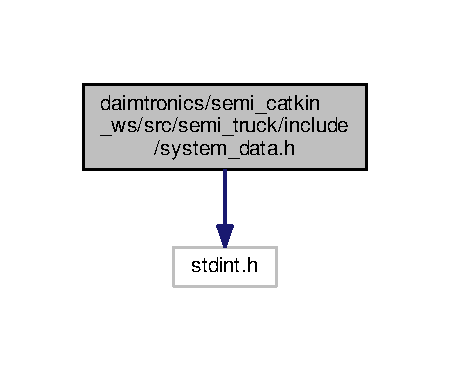
\includegraphics[width=216pt]{semi__catkin__ws_2src_2semi__truck_2include_2system__data_8h__incl}
\end{center}
\end{figure}
\subsection*{Classes}
\begin{DoxyCompactItemize}
\item 
struct \hyperlink{structsystem__data__t}{system\+\_\+data\+\_\+t}
\end{DoxyCompactItemize}

\hypertarget{teensy__chibios_2src_2main_2include_2system__data_8h}{}\section{daimtronics/teensy\+\_\+chibios/src/main/include/system\+\_\+data.h File Reference}
\label{teensy__chibios_2src_2main_2include_2system__data_8h}\index{daimtronics/teensy\+\_\+chibios/src/main/include/system\+\_\+data.\+h@{daimtronics/teensy\+\_\+chibios/src/main/include/system\+\_\+data.\+h}}
{\ttfamily \#include $<$stdint.\+h$>$}\\*
Include dependency graph for system\+\_\+data.\+h\+:
\nopagebreak
\begin{figure}[H]
\begin{center}
\leavevmode
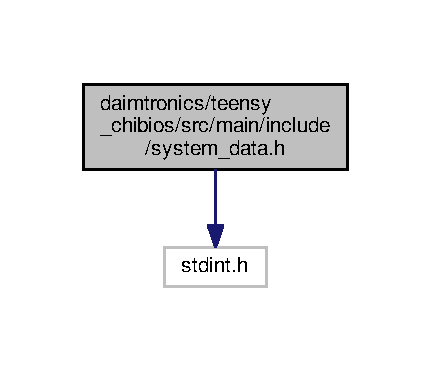
\includegraphics[width=207pt]{teensy__chibios_2src_2main_2include_2system__data_8h__incl}
\end{center}
\end{figure}
This graph shows which files directly or indirectly include this file\+:
\nopagebreak
\begin{figure}[H]
\begin{center}
\leavevmode
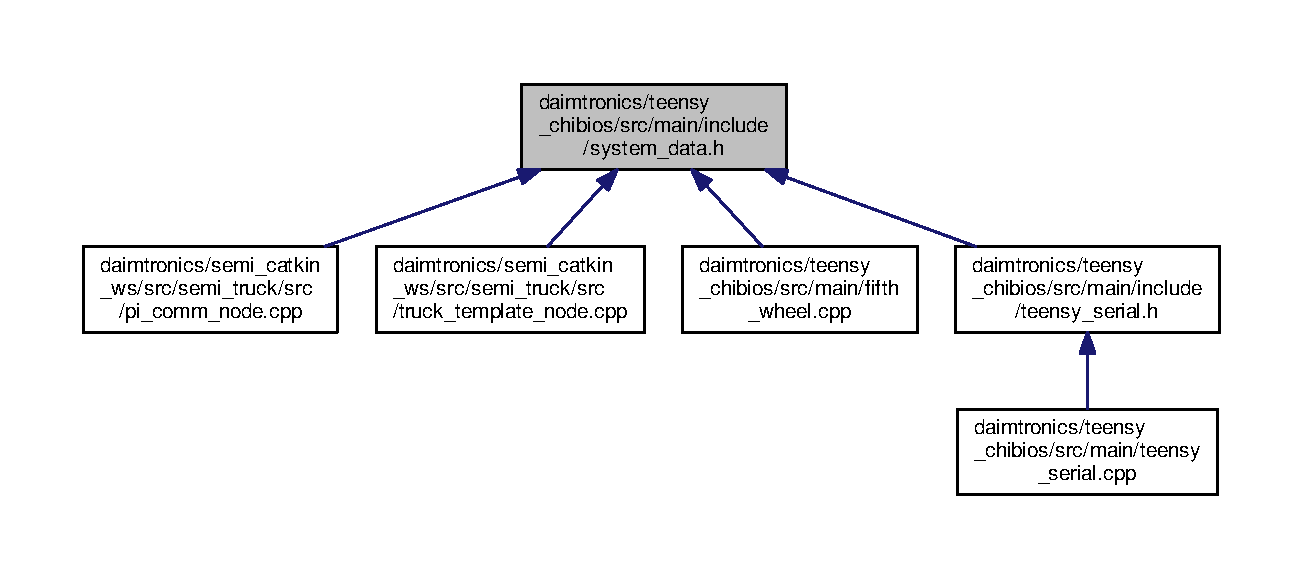
\includegraphics[width=350pt]{teensy__chibios_2src_2main_2include_2system__data_8h__dep__incl}
\end{center}
\end{figure}
\subsection*{Classes}
\begin{DoxyCompactItemize}
\item 
struct \hyperlink{structsensor__data__t}{sensor\+\_\+data\+\_\+t}
\item 
struct \hyperlink{structactuator__data__t}{actuator\+\_\+data\+\_\+t}
\item 
struct \hyperlink{structsystem__data__t}{system\+\_\+data\+\_\+t}
\end{DoxyCompactItemize}
\subsection*{Typedefs}
\begin{DoxyCompactItemize}
\item 
typedef struct \hyperlink{structsensor__data__t}{sensor\+\_\+data\+\_\+t} \hyperlink{teensy__chibios_2src_2main_2include_2system__data_8h_ac544068a1e6844fd0bbd13538265a805}{sensor\+\_\+data\+\_\+t}
\item 
typedef struct \hyperlink{structactuator__data__t}{actuator\+\_\+data\+\_\+t} \hyperlink{teensy__chibios_2src_2main_2include_2system__data_8h_ac7d45ee3657481870de05092f3c04c45}{actuator\+\_\+data\+\_\+t}
\item 
typedef struct \hyperlink{structsystem__data__t}{system\+\_\+data\+\_\+t} \hyperlink{teensy__chibios_2src_2main_2include_2system__data_8h_abfa04c60d7a7c1d2d5ce2fb3c83cd976}{system\+\_\+data\+\_\+t}
\end{DoxyCompactItemize}


\subsection{Typedef Documentation}
\index{teensy\+\_\+chibios/src/main/include/system\+\_\+data.\+h@{teensy\+\_\+chibios/src/main/include/system\+\_\+data.\+h}!actuator\+\_\+data\+\_\+t@{actuator\+\_\+data\+\_\+t}}
\index{actuator\+\_\+data\+\_\+t@{actuator\+\_\+data\+\_\+t}!teensy\+\_\+chibios/src/main/include/system\+\_\+data.\+h@{teensy\+\_\+chibios/src/main/include/system\+\_\+data.\+h}}
\subsubsection[{\texorpdfstring{actuator\+\_\+data\+\_\+t}{actuator_data_t}}]{\setlength{\rightskip}{0pt plus 5cm}typedef struct {\bf actuator\+\_\+data\+\_\+t}  {\bf actuator\+\_\+data\+\_\+t}}\hypertarget{teensy__chibios_2src_2main_2include_2system__data_8h_ac7d45ee3657481870de05092f3c04c45}{}\label{teensy__chibios_2src_2main_2include_2system__data_8h_ac7d45ee3657481870de05092f3c04c45}
\index{teensy\+\_\+chibios/src/main/include/system\+\_\+data.\+h@{teensy\+\_\+chibios/src/main/include/system\+\_\+data.\+h}!sensor\+\_\+data\+\_\+t@{sensor\+\_\+data\+\_\+t}}
\index{sensor\+\_\+data\+\_\+t@{sensor\+\_\+data\+\_\+t}!teensy\+\_\+chibios/src/main/include/system\+\_\+data.\+h@{teensy\+\_\+chibios/src/main/include/system\+\_\+data.\+h}}
\subsubsection[{\texorpdfstring{sensor\+\_\+data\+\_\+t}{sensor_data_t}}]{\setlength{\rightskip}{0pt plus 5cm}typedef struct {\bf sensor\+\_\+data\+\_\+t}  {\bf sensor\+\_\+data\+\_\+t}}\hypertarget{teensy__chibios_2src_2main_2include_2system__data_8h_ac544068a1e6844fd0bbd13538265a805}{}\label{teensy__chibios_2src_2main_2include_2system__data_8h_ac544068a1e6844fd0bbd13538265a805}
\index{teensy\+\_\+chibios/src/main/include/system\+\_\+data.\+h@{teensy\+\_\+chibios/src/main/include/system\+\_\+data.\+h}!system\+\_\+data\+\_\+t@{system\+\_\+data\+\_\+t}}
\index{system\+\_\+data\+\_\+t@{system\+\_\+data\+\_\+t}!teensy\+\_\+chibios/src/main/include/system\+\_\+data.\+h@{teensy\+\_\+chibios/src/main/include/system\+\_\+data.\+h}}
\subsubsection[{\texorpdfstring{system\+\_\+data\+\_\+t}{system_data_t}}]{\setlength{\rightskip}{0pt plus 5cm}typedef struct {\bf system\+\_\+data\+\_\+t}  {\bf system\+\_\+data\+\_\+t}}\hypertarget{teensy__chibios_2src_2main_2include_2system__data_8h_abfa04c60d7a7c1d2d5ce2fb3c83cd976}{}\label{teensy__chibios_2src_2main_2include_2system__data_8h_abfa04c60d7a7c1d2d5ce2fb3c83cd976}

\hypertarget{_teensy___actuators_8h}{}\section{daimtronics/semi\+\_\+catkin\+\_\+ws/src/semi\+\_\+truck/include/\+Teensy\+\_\+\+Actuators.h File Reference}
\label{_teensy___actuators_8h}\index{daimtronics/semi\+\_\+catkin\+\_\+ws/src/semi\+\_\+truck/include/\+Teensy\+\_\+\+Actuators.\+h@{daimtronics/semi\+\_\+catkin\+\_\+ws/src/semi\+\_\+truck/include/\+Teensy\+\_\+\+Actuators.\+h}}
{\ttfamily \#include $<$string$>$}\\*
{\ttfamily \#include $<$vector$>$}\\*
{\ttfamily \#include $<$map$>$}\\*
{\ttfamily \#include $<$ros/types.\+h$>$}\\*
{\ttfamily \#include $<$ros/serialization.\+h$>$}\\*
{\ttfamily \#include $<$ros/builtin\+\_\+message\+\_\+traits.\+h$>$}\\*
{\ttfamily \#include $<$ros/message\+\_\+operations.\+h$>$}\\*
Include dependency graph for Teensy\+\_\+\+Actuators.\+h\+:
\nopagebreak
\begin{figure}[H]
\begin{center}
\leavevmode
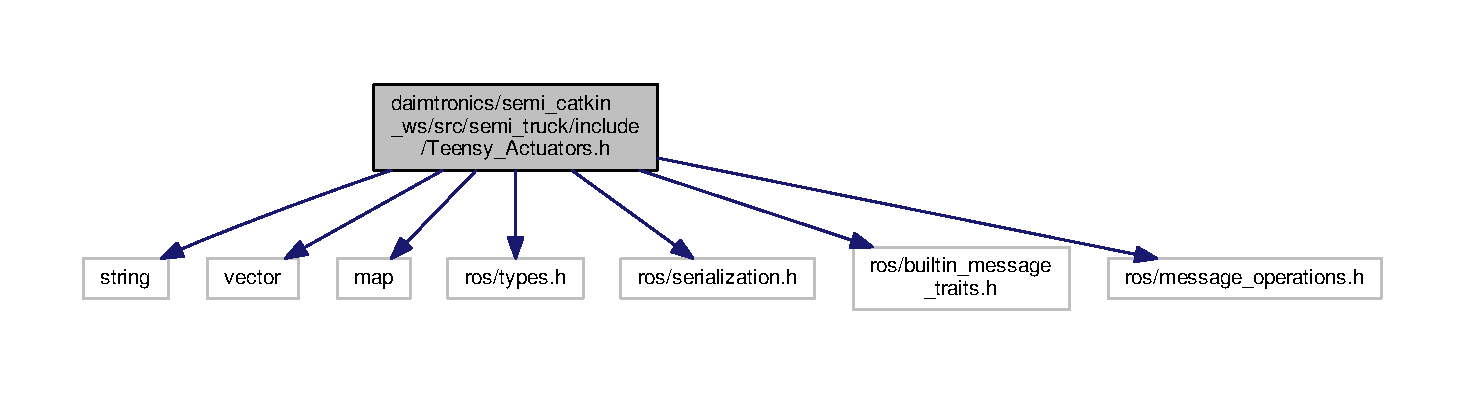
\includegraphics[width=350pt]{_teensy___actuators_8h__incl}
\end{center}
\end{figure}
This graph shows which files directly or indirectly include this file\+:
\nopagebreak
\begin{figure}[H]
\begin{center}
\leavevmode
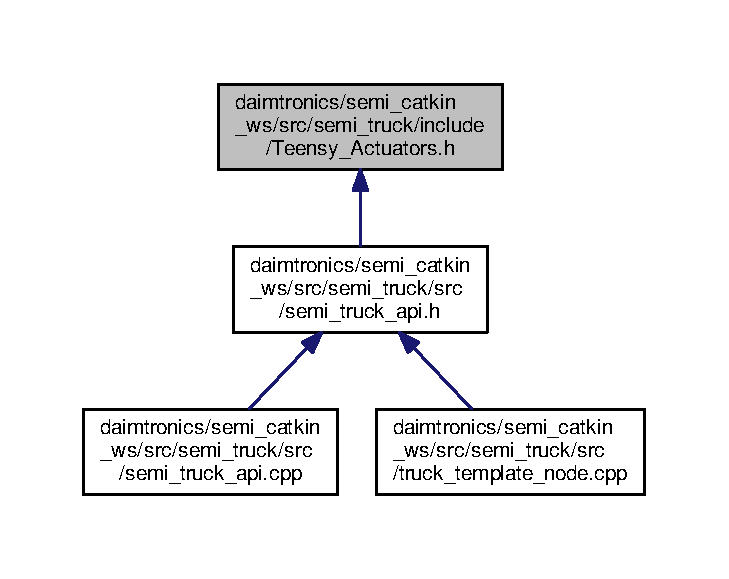
\includegraphics[width=350pt]{_teensy___actuators_8h__dep__incl}
\end{center}
\end{figure}
\subsection*{Classes}
\begin{DoxyCompactItemize}
\item 
struct \hyperlink{structsemi__truck_1_1_teensy___actuators__}{semi\+\_\+truck\+::\+Teensy\+\_\+\+Actuators\+\_\+$<$ Container\+Allocator $>$}
\item 
struct \hyperlink{structros_1_1message__traits_1_1_is_fixed_size_3_01_1_1semi__truck_1_1_teensy___actuators___3_01_container_allocator_01_4_01_4}{ros\+::message\+\_\+traits\+::\+Is\+Fixed\+Size$<$ \+::semi\+\_\+truck\+::\+Teensy\+\_\+\+Actuators\+\_\+$<$ Container\+Allocator $>$ $>$}
\item 
struct \hyperlink{structros_1_1message__traits_1_1_is_fixed_size_3_01_1_1semi__truck_1_1_teensy___actuators___3_01e88fb587a6d6e04d6a7968cdf33bb127}{ros\+::message\+\_\+traits\+::\+Is\+Fixed\+Size$<$ \+::semi\+\_\+truck\+::\+Teensy\+\_\+\+Actuators\+\_\+$<$ Container\+Allocator $>$ const  $>$}
\item 
struct \hyperlink{structros_1_1message__traits_1_1_is_message_3_01_1_1semi__truck_1_1_teensy___actuators___3_01_container_allocator_01_4_01_4}{ros\+::message\+\_\+traits\+::\+Is\+Message$<$ \+::semi\+\_\+truck\+::\+Teensy\+\_\+\+Actuators\+\_\+$<$ Container\+Allocator $>$ $>$}
\item 
struct \hyperlink{structros_1_1message__traits_1_1_is_message_3_01_1_1semi__truck_1_1_teensy___actuators___3_01_cobc29fbe598d16bac74a311be55406c9e}{ros\+::message\+\_\+traits\+::\+Is\+Message$<$ \+::semi\+\_\+truck\+::\+Teensy\+\_\+\+Actuators\+\_\+$<$ Container\+Allocator $>$ const  $>$}
\item 
struct \hyperlink{structros_1_1message__traits_1_1_has_header_3_01_1_1semi__truck_1_1_teensy___actuators___3_01_container_allocator_01_4_01_4}{ros\+::message\+\_\+traits\+::\+Has\+Header$<$ \+::semi\+\_\+truck\+::\+Teensy\+\_\+\+Actuators\+\_\+$<$ Container\+Allocator $>$ $>$}
\item 
struct \hyperlink{structros_1_1message__traits_1_1_has_header_3_01_1_1semi__truck_1_1_teensy___actuators___3_01_coe86513e6694fc989720644eb04b2c486}{ros\+::message\+\_\+traits\+::\+Has\+Header$<$ \+::semi\+\_\+truck\+::\+Teensy\+\_\+\+Actuators\+\_\+$<$ Container\+Allocator $>$ const  $>$}
\item 
struct \hyperlink{structros_1_1message__traits_1_1_m_d5_sum_3_01_1_1semi__truck_1_1_teensy___actuators___3_01_container_allocator_01_4_01_4}{ros\+::message\+\_\+traits\+::\+M\+D5\+Sum$<$ \+::semi\+\_\+truck\+::\+Teensy\+\_\+\+Actuators\+\_\+$<$ Container\+Allocator $>$ $>$}
\item 
struct \hyperlink{structros_1_1message__traits_1_1_data_type_3_01_1_1semi__truck_1_1_teensy___actuators___3_01_container_allocator_01_4_01_4}{ros\+::message\+\_\+traits\+::\+Data\+Type$<$ \+::semi\+\_\+truck\+::\+Teensy\+\_\+\+Actuators\+\_\+$<$ Container\+Allocator $>$ $>$}
\item 
struct \hyperlink{structros_1_1message__traits_1_1_definition_3_01_1_1semi__truck_1_1_teensy___actuators___3_01_container_allocator_01_4_01_4}{ros\+::message\+\_\+traits\+::\+Definition$<$ \+::semi\+\_\+truck\+::\+Teensy\+\_\+\+Actuators\+\_\+$<$ Container\+Allocator $>$ $>$}
\item 
struct \hyperlink{structros_1_1serialization_1_1_serializer_3_01_1_1semi__truck_1_1_teensy___actuators___3_01_container_allocator_01_4_01_4}{ros\+::serialization\+::\+Serializer$<$ \+::semi\+\_\+truck\+::\+Teensy\+\_\+\+Actuators\+\_\+$<$ Container\+Allocator $>$ $>$}
\item 
struct \hyperlink{structros_1_1message__operations_1_1_printer_3_01_1_1semi__truck_1_1_teensy___actuators___3_01_container_allocator_01_4_01_4}{ros\+::message\+\_\+operations\+::\+Printer$<$ \+::semi\+\_\+truck\+::\+Teensy\+\_\+\+Actuators\+\_\+$<$ Container\+Allocator $>$ $>$}
\end{DoxyCompactItemize}
\subsection*{Namespaces}
\begin{DoxyCompactItemize}
\item 
 \hyperlink{namespacesemi__truck}{semi\+\_\+truck}
\item 
 \hyperlink{namespaceros}{ros}
\item 
 \hyperlink{namespaceros_1_1message__traits}{ros\+::message\+\_\+traits}
\item 
 \hyperlink{namespaceros_1_1serialization}{ros\+::serialization}
\item 
 \hyperlink{namespaceros_1_1message__operations}{ros\+::message\+\_\+operations}
\end{DoxyCompactItemize}
\subsection*{Typedefs}
\begin{DoxyCompactItemize}
\item 
typedef \+::\hyperlink{structsemi__truck_1_1_teensy___actuators__}{semi\+\_\+truck\+::\+Teensy\+\_\+\+Actuators\+\_\+}$<$ std\+::allocator$<$ void $>$ $>$ \hyperlink{namespacesemi__truck_ab8254dd176d8fef1f1381fb4e7e5e869}{semi\+\_\+truck\+::\+Teensy\+\_\+\+Actuators}
\item 
typedef boost\+::shared\+\_\+ptr$<$ \+::\hyperlink{namespacesemi__truck_ab8254dd176d8fef1f1381fb4e7e5e869}{semi\+\_\+truck\+::\+Teensy\+\_\+\+Actuators} $>$ \hyperlink{namespacesemi__truck_a865760e0f4929063a89f6acce25f9bab}{semi\+\_\+truck\+::\+Teensy\+\_\+\+Actuators\+Ptr}
\item 
typedef boost\+::shared\+\_\+ptr$<$ \+::\hyperlink{namespacesemi__truck_ab8254dd176d8fef1f1381fb4e7e5e869}{semi\+\_\+truck\+::\+Teensy\+\_\+\+Actuators} const  $>$ \hyperlink{namespacesemi__truck_a66fc29d018a09cb82a509c3de393001b}{semi\+\_\+truck\+::\+Teensy\+\_\+\+Actuators\+Const\+Ptr}
\end{DoxyCompactItemize}
\subsection*{Functions}
\begin{DoxyCompactItemize}
\item 
{\footnotesize template$<$typename Container\+Allocator $>$ }\\std\+::ostream \& \hyperlink{namespacesemi__truck_aa64782c2c0f1112e9c802016c4e3d4b3}{semi\+\_\+truck\+::operator$<$$<$} (std\+::ostream \&s, const \+::\hyperlink{structsemi__truck_1_1_teensy___actuators__}{semi\+\_\+truck\+::\+Teensy\+\_\+\+Actuators\+\_\+}$<$ Container\+Allocator $>$ \&v)
\end{DoxyCompactItemize}

\hypertarget{_teensy___sensors_8h}{}\section{daimtronics/semi\+\_\+catkin\+\_\+ws/src/semi\+\_\+truck/include/\+Teensy\+\_\+\+Sensors.h File Reference}
\label{_teensy___sensors_8h}\index{daimtronics/semi\+\_\+catkin\+\_\+ws/src/semi\+\_\+truck/include/\+Teensy\+\_\+\+Sensors.\+h@{daimtronics/semi\+\_\+catkin\+\_\+ws/src/semi\+\_\+truck/include/\+Teensy\+\_\+\+Sensors.\+h}}
{\ttfamily \#include $<$string$>$}\\*
{\ttfamily \#include $<$vector$>$}\\*
{\ttfamily \#include $<$map$>$}\\*
{\ttfamily \#include $<$ros/types.\+h$>$}\\*
{\ttfamily \#include $<$ros/serialization.\+h$>$}\\*
{\ttfamily \#include $<$ros/builtin\+\_\+message\+\_\+traits.\+h$>$}\\*
{\ttfamily \#include $<$ros/message\+\_\+operations.\+h$>$}\\*
Include dependency graph for Teensy\+\_\+\+Sensors.\+h\+:
\nopagebreak
\begin{figure}[H]
\begin{center}
\leavevmode
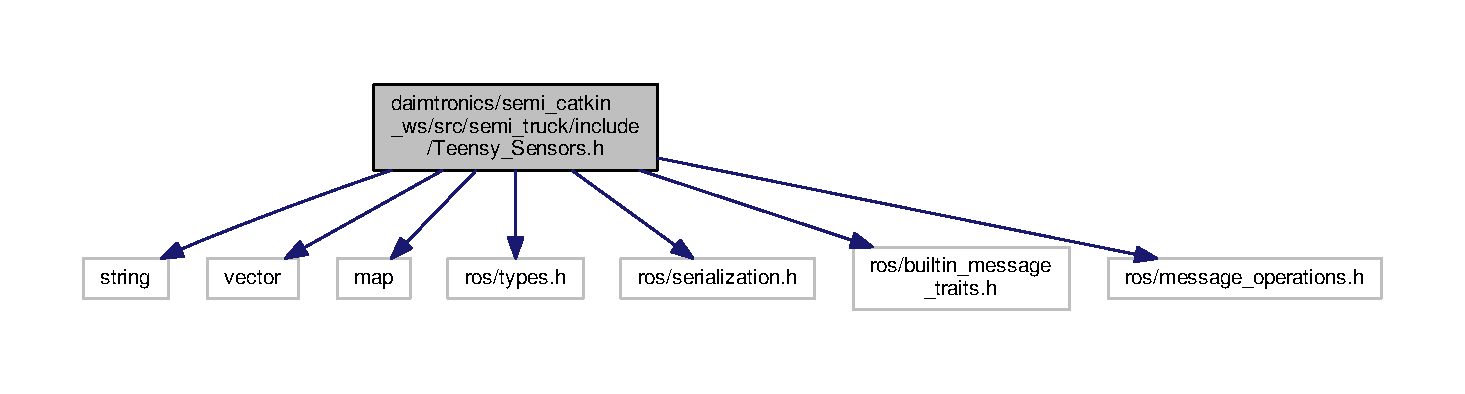
\includegraphics[width=350pt]{_teensy___sensors_8h__incl}
\end{center}
\end{figure}
This graph shows which files directly or indirectly include this file\+:
\nopagebreak
\begin{figure}[H]
\begin{center}
\leavevmode
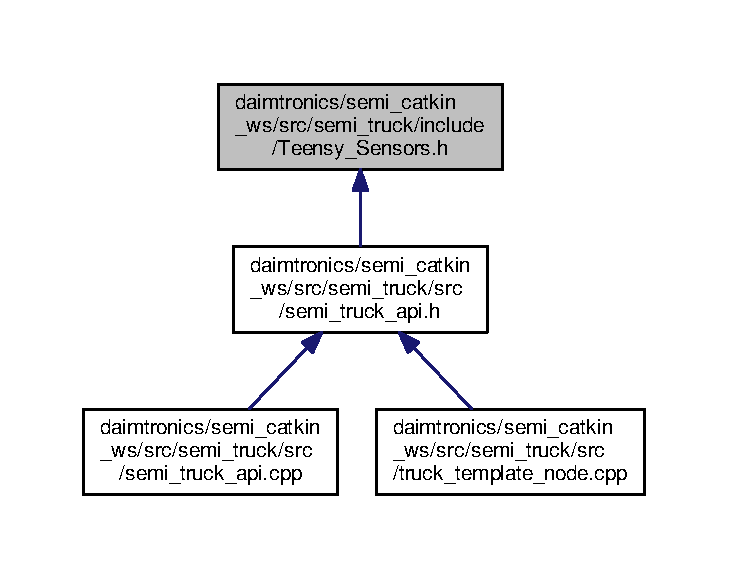
\includegraphics[width=350pt]{_teensy___sensors_8h__dep__incl}
\end{center}
\end{figure}
\subsection*{Classes}
\begin{DoxyCompactItemize}
\item 
struct \hyperlink{structsemi__truck_1_1_teensy___sensors__}{semi\+\_\+truck\+::\+Teensy\+\_\+\+Sensors\+\_\+$<$ Container\+Allocator $>$}
\item 
struct \hyperlink{structros_1_1message__traits_1_1_is_fixed_size_3_01_1_1semi__truck_1_1_teensy___sensors___3_01_container_allocator_01_4_01_4}{ros\+::message\+\_\+traits\+::\+Is\+Fixed\+Size$<$ \+::semi\+\_\+truck\+::\+Teensy\+\_\+\+Sensors\+\_\+$<$ Container\+Allocator $>$ $>$}
\item 
struct \hyperlink{structros_1_1message__traits_1_1_is_fixed_size_3_01_1_1semi__truck_1_1_teensy___sensors___3_01_cb53d5848a141775744a1974dc7127755}{ros\+::message\+\_\+traits\+::\+Is\+Fixed\+Size$<$ \+::semi\+\_\+truck\+::\+Teensy\+\_\+\+Sensors\+\_\+$<$ Container\+Allocator $>$ const  $>$}
\item 
struct \hyperlink{structros_1_1message__traits_1_1_is_message_3_01_1_1semi__truck_1_1_teensy___sensors___3_01_container_allocator_01_4_01_4}{ros\+::message\+\_\+traits\+::\+Is\+Message$<$ \+::semi\+\_\+truck\+::\+Teensy\+\_\+\+Sensors\+\_\+$<$ Container\+Allocator $>$ $>$}
\item 
struct \hyperlink{structros_1_1message__traits_1_1_is_message_3_01_1_1semi__truck_1_1_teensy___sensors___3_01_contee20f324312af52498809118a40cc274}{ros\+::message\+\_\+traits\+::\+Is\+Message$<$ \+::semi\+\_\+truck\+::\+Teensy\+\_\+\+Sensors\+\_\+$<$ Container\+Allocator $>$ const  $>$}
\item 
struct \hyperlink{structros_1_1message__traits_1_1_has_header_3_01_1_1semi__truck_1_1_teensy___sensors___3_01_container_allocator_01_4_01_4}{ros\+::message\+\_\+traits\+::\+Has\+Header$<$ \+::semi\+\_\+truck\+::\+Teensy\+\_\+\+Sensors\+\_\+$<$ Container\+Allocator $>$ $>$}
\item 
struct \hyperlink{structros_1_1message__traits_1_1_has_header_3_01_1_1semi__truck_1_1_teensy___sensors___3_01_cont27420888fce5a6e96344b08bcfbbf57b}{ros\+::message\+\_\+traits\+::\+Has\+Header$<$ \+::semi\+\_\+truck\+::\+Teensy\+\_\+\+Sensors\+\_\+$<$ Container\+Allocator $>$ const  $>$}
\item 
struct \hyperlink{structros_1_1message__traits_1_1_m_d5_sum_3_01_1_1semi__truck_1_1_teensy___sensors___3_01_container_allocator_01_4_01_4}{ros\+::message\+\_\+traits\+::\+M\+D5\+Sum$<$ \+::semi\+\_\+truck\+::\+Teensy\+\_\+\+Sensors\+\_\+$<$ Container\+Allocator $>$ $>$}
\item 
struct \hyperlink{structros_1_1message__traits_1_1_data_type_3_01_1_1semi__truck_1_1_teensy___sensors___3_01_container_allocator_01_4_01_4}{ros\+::message\+\_\+traits\+::\+Data\+Type$<$ \+::semi\+\_\+truck\+::\+Teensy\+\_\+\+Sensors\+\_\+$<$ Container\+Allocator $>$ $>$}
\item 
struct \hyperlink{structros_1_1message__traits_1_1_definition_3_01_1_1semi__truck_1_1_teensy___sensors___3_01_container_allocator_01_4_01_4}{ros\+::message\+\_\+traits\+::\+Definition$<$ \+::semi\+\_\+truck\+::\+Teensy\+\_\+\+Sensors\+\_\+$<$ Container\+Allocator $>$ $>$}
\item 
struct \hyperlink{structros_1_1serialization_1_1_serializer_3_01_1_1semi__truck_1_1_teensy___sensors___3_01_container_allocator_01_4_01_4}{ros\+::serialization\+::\+Serializer$<$ \+::semi\+\_\+truck\+::\+Teensy\+\_\+\+Sensors\+\_\+$<$ Container\+Allocator $>$ $>$}
\item 
struct \hyperlink{structros_1_1message__operations_1_1_printer_3_01_1_1semi__truck_1_1_teensy___sensors___3_01_container_allocator_01_4_01_4}{ros\+::message\+\_\+operations\+::\+Printer$<$ \+::semi\+\_\+truck\+::\+Teensy\+\_\+\+Sensors\+\_\+$<$ Container\+Allocator $>$ $>$}
\end{DoxyCompactItemize}
\subsection*{Namespaces}
\begin{DoxyCompactItemize}
\item 
 \hyperlink{namespacesemi__truck}{semi\+\_\+truck}
\item 
 \hyperlink{namespaceros}{ros}
\item 
 \hyperlink{namespaceros_1_1message__traits}{ros\+::message\+\_\+traits}
\item 
 \hyperlink{namespaceros_1_1serialization}{ros\+::serialization}
\item 
 \hyperlink{namespaceros_1_1message__operations}{ros\+::message\+\_\+operations}
\end{DoxyCompactItemize}
\subsection*{Typedefs}
\begin{DoxyCompactItemize}
\item 
typedef \+::\hyperlink{structsemi__truck_1_1_teensy___sensors__}{semi\+\_\+truck\+::\+Teensy\+\_\+\+Sensors\+\_\+}$<$ std\+::allocator$<$ void $>$ $>$ \hyperlink{namespacesemi__truck_a8ffe15bf9a1e739c2242ac6d6feaa67f}{semi\+\_\+truck\+::\+Teensy\+\_\+\+Sensors}
\item 
typedef boost\+::shared\+\_\+ptr$<$ \+::\hyperlink{namespacesemi__truck_a8ffe15bf9a1e739c2242ac6d6feaa67f}{semi\+\_\+truck\+::\+Teensy\+\_\+\+Sensors} $>$ \hyperlink{namespacesemi__truck_a2e84194604862e88522a06e29cff3b7e}{semi\+\_\+truck\+::\+Teensy\+\_\+\+Sensors\+Ptr}
\item 
typedef boost\+::shared\+\_\+ptr$<$ \+::\hyperlink{namespacesemi__truck_a8ffe15bf9a1e739c2242ac6d6feaa67f}{semi\+\_\+truck\+::\+Teensy\+\_\+\+Sensors} const  $>$ \hyperlink{namespacesemi__truck_a47fa34135a8e2aa8c828d29436a9c726}{semi\+\_\+truck\+::\+Teensy\+\_\+\+Sensors\+Const\+Ptr}
\end{DoxyCompactItemize}
\subsection*{Functions}
\begin{DoxyCompactItemize}
\item 
{\footnotesize template$<$typename Container\+Allocator $>$ }\\std\+::ostream \& \hyperlink{namespacesemi__truck_a1bb38ca9af123f5a2cd3ab871f6618d2}{semi\+\_\+truck\+::operator$<$$<$} (std\+::ostream \&s, const \+::\hyperlink{structsemi__truck_1_1_teensy___sensors__}{semi\+\_\+truck\+::\+Teensy\+\_\+\+Sensors\+\_\+}$<$ Container\+Allocator $>$ \&v)
\end{DoxyCompactItemize}

\hypertarget{_teensy___actuators_8msg}{}\section{daimtronics/semi\+\_\+catkin\+\_\+ws/src/semi\+\_\+truck/msg/\+Teensy\+\_\+\+Actuators.msg File Reference}
\label{_teensy___actuators_8msg}\index{daimtronics/semi\+\_\+catkin\+\_\+ws/src/semi\+\_\+truck/msg/\+Teensy\+\_\+\+Actuators.\+msg@{daimtronics/semi\+\_\+catkin\+\_\+ws/src/semi\+\_\+truck/msg/\+Teensy\+\_\+\+Actuators.\+msg}}

\hypertarget{_teensy___sensors_8msg}{}\section{daimtronics/semi\+\_\+catkin\+\_\+ws/src/semi\+\_\+truck/msg/\+Teensy\+\_\+\+Sensors.msg File Reference}
\label{_teensy___sensors_8msg}\index{daimtronics/semi\+\_\+catkin\+\_\+ws/src/semi\+\_\+truck/msg/\+Teensy\+\_\+\+Sensors.\+msg@{daimtronics/semi\+\_\+catkin\+\_\+ws/src/semi\+\_\+truck/msg/\+Teensy\+\_\+\+Sensors.\+msg}}

\hypertarget{package_8xml}{}\section{daimtronics/semi\+\_\+catkin\+\_\+ws/src/semi\+\_\+truck/package.xml File Reference}
\label{package_8xml}\index{daimtronics/semi\+\_\+catkin\+\_\+ws/src/semi\+\_\+truck/package.\+xml@{daimtronics/semi\+\_\+catkin\+\_\+ws/src/semi\+\_\+truck/package.\+xml}}

\hypertarget{pi__comm__node_8cpp}{}\section{daimtronics/semi\+\_\+catkin\+\_\+ws/src/semi\+\_\+truck/src/pi\+\_\+comm\+\_\+node.cpp File Reference}
\label{pi__comm__node_8cpp}\index{daimtronics/semi\+\_\+catkin\+\_\+ws/src/semi\+\_\+truck/src/pi\+\_\+comm\+\_\+node.\+cpp@{daimtronics/semi\+\_\+catkin\+\_\+ws/src/semi\+\_\+truck/src/pi\+\_\+comm\+\_\+node.\+cpp}}
{\ttfamily \#include \char`\"{}pi\+\_\+comm\+\_\+node.\+h\char`\"{}}\\*
{\ttfamily \#include \char`\"{}system\+\_\+data.\+h\char`\"{}}\\*
{\ttfamily \#include \char`\"{}semi\+\_\+truck/\+Teensy\+\_\+\+Sensors.\+h\char`\"{}}\\*
{\ttfamily \#include \char`\"{}semi\+\_\+truck/\+Teensy\+\_\+\+Actuators.\+h\char`\"{}}\\*
{\ttfamily \#include $<$wiring\+Serial.\+h$>$}\\*
{\ttfamily \#include $<$wiring\+Pi.\+h$>$}\\*
{\ttfamily \#include $<$stdio.\+h$>$}\\*
{\ttfamily \#include $<$unistd.\+h$>$}\\*
{\ttfamily \#include $<$ros/ros.\+h$>$}\\*
{\ttfamily \#include $<$sensor\+\_\+msgs/\+Laser\+Scan.\+h$>$}\\*
Include dependency graph for pi\+\_\+comm\+\_\+node.\+cpp\+:
\nopagebreak
\begin{figure}[H]
\begin{center}
\leavevmode
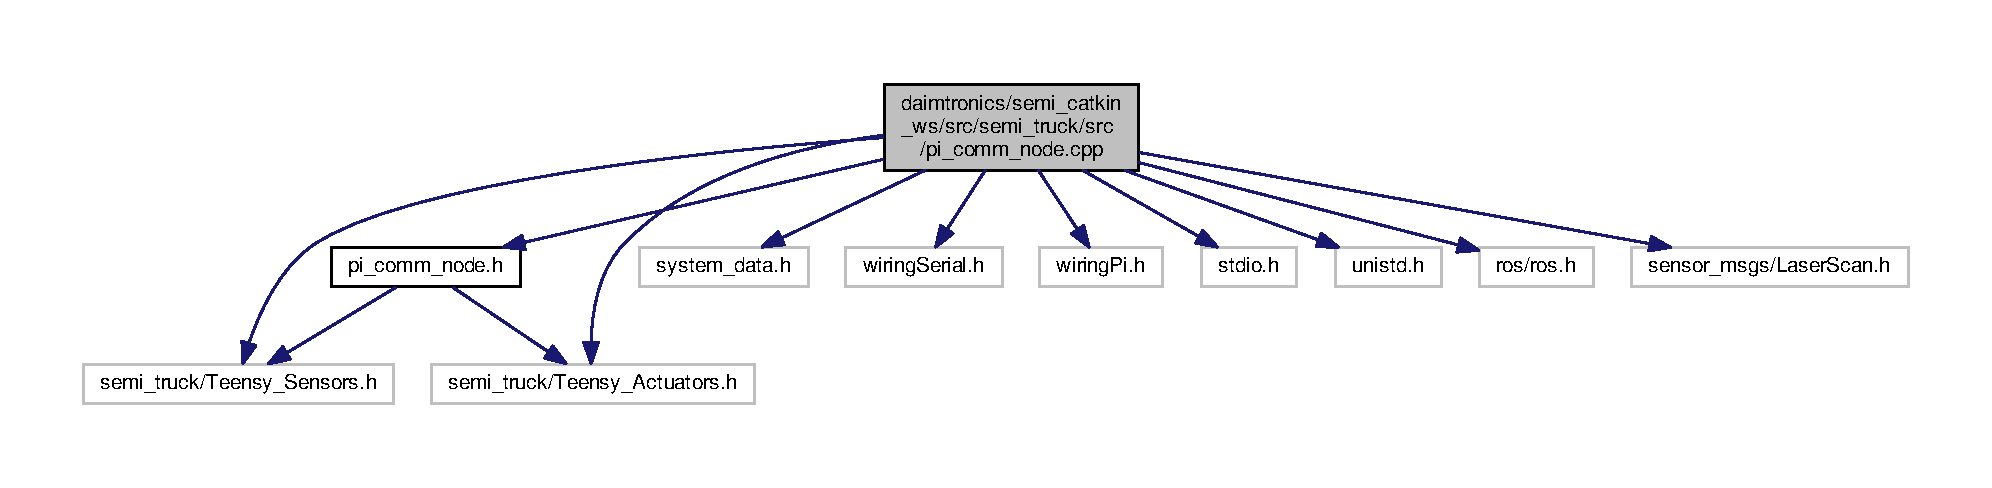
\includegraphics[width=350pt]{pi__comm__node_8cpp__incl}
\end{center}
\end{figure}
\subsection*{Macros}
\begin{DoxyCompactItemize}
\item 
\#define \hyperlink{pi__comm__node_8cpp_adeb5281b5f526ce88376cb4b4b36572e}{S\+H\+O\+R\+T\+\_\+\+S\+I\+ZE}~2
\item 
\#define \hyperlink{pi__comm__node_8cpp_a86a25f62b3f5ba49be747ef1990fe00b}{R\+E\+L\+A\+Y\+\_\+\+P\+I\+N\+\_\+1}~7
\item 
\#define \hyperlink{pi__comm__node_8cpp_afabf4690ae765da1178317f69b6de417}{R\+E\+L\+A\+Y\+\_\+\+P\+I\+N\+\_\+2}~0
\item 
\#define \hyperlink{pi__comm__node_8cpp_a7e041c16acda3d982a2c6c1d0ab78fd7}{S\+Y\+N\+C\+\_\+\+V\+A\+L\+UE}~-\/32000
\item 
\#define \hyperlink{pi__comm__node_8cpp_a70beb8afe59e7dcd578884cdbc0e231b}{S\+E\+N\+S\+O\+R\+\_\+\+D\+A\+T\+A\+\_\+\+S\+I\+Z\+E\+\_\+\+W\+\_\+\+S\+Y\+NC}~14
\item 
\#define \hyperlink{pi__comm__node_8cpp_a148c44e2e5bb295e12c94b137e9717a7}{S\+E\+N\+S\+O\+R\+\_\+\+D\+A\+T\+A\+\_\+\+S\+I\+ZE}~12
\item 
\#define \hyperlink{pi__comm__node_8cpp_af7cb12b462b4594bd759d1b4e241ec4c}{U\+A\+RT}~\char`\"{}/dev/tty\+S0\char`\"{}
\item 
\#define \hyperlink{pi__comm__node_8cpp_a734bbab06e1a9fd2e5522db0221ff6e3}{B\+A\+U\+D\+R\+A\+TE}~9600
\item 
\#define \hyperlink{pi__comm__node_8cpp_aa77ad76fb0e0966b273db92f13af4429}{L\+O\+O\+P\+\_\+\+F\+R\+E\+Q\+U\+E\+N\+CY}~20
\end{DoxyCompactItemize}
\subsection*{Functions}
\begin{DoxyCompactItemize}
\item 
int \hyperlink{pi__comm__node_8cpp_a3c04138a5bfe5d72780bb7e82a18e627}{main} (int argc, char $\ast$$\ast$argv)
\begin{DoxyCompactList}\small\item\em The main function for the R\+OS node to communicate with the Teensy over U\+A\+RT. It receives sensor data from the Teensy and publishes this data to the teensy\+\_\+sensor\+\_\+data topic. It also subscribes to the teensy\+\_\+actuator\+\_\+data topic and writes the values it gets to the Teensy over U\+A\+RT. \end{DoxyCompactList}\item 
void \hyperlink{pi__comm__node_8cpp_a1c868413212badac680da7f573eb6be4}{pi\+\_\+sync} ()
\begin{DoxyCompactList}\small\item\em Called before reading sensor data from the Teensy. It will read the buffer until it encounters the S\+Y\+N\+C\+\_\+\+V\+A\+L\+UE that has been defined. Once this happens, the next set of bytes are the set of sensor values. \end{DoxyCompactList}\item 
short \hyperlink{pi__comm__node_8cpp_a41b126a0cd4632cb40a651336b009cf5}{read\+\_\+sensor\+\_\+msg} (int serial, char num\+\_\+bytes)
\begin{DoxyCompactList}\small\item\em Reads a single value from the U\+A\+RT communication buffer. \end{DoxyCompactList}\item 
void \hyperlink{pi__comm__node_8cpp_a0c5cd860a6d8f747aea77d78d2e8bb7c}{read\+\_\+from\+\_\+teensy} (int serial, \hyperlink{namespacesemi__truck_a8ffe15bf9a1e739c2242ac6d6feaa67f}{semi\+\_\+truck\+::\+Teensy\+\_\+\+Sensors} \&sensors)
\begin{DoxyCompactList}\small\item\em Reads an entire set of Teensy sensor data by calling read\+\_\+sensor\+\_\+msg on each sensor data in the U\+A\+RT message. \end{DoxyCompactList}\item 
void \hyperlink{pi__comm__node_8cpp_a0cdc366bcb9df6f3489878319738c3cd}{write\+\_\+actuator\+\_\+msg} (int serial, short actuator\+\_\+val, char num\+\_\+bytes)
\begin{DoxyCompactList}\small\item\em Writes a single actuator value to the Teensy. \end{DoxyCompactList}\item 
void \hyperlink{pi__comm__node_8cpp_af969dff0aa66a4e3c813f09b452050cc}{write\+\_\+to\+\_\+teensy} (int serial, const \hyperlink{namespacesemi__truck_ab8254dd176d8fef1f1381fb4e7e5e869}{semi\+\_\+truck\+::\+Teensy\+\_\+\+Actuators} \&actuators)
\begin{DoxyCompactList}\small\item\em Writes an entire set of actuator data to the Teensy via U\+A\+RT. \end{DoxyCompactList}\item 
void \hyperlink{pi__comm__node_8cpp_a25959d1c80ccb8a385982b0cec8750fb}{print\+\_\+sensors} (const \hyperlink{namespacesemi__truck_a8ffe15bf9a1e739c2242ac6d6feaa67f}{semi\+\_\+truck\+::\+Teensy\+\_\+\+Sensors} \&sensors)
\begin{DoxyCompactList}\small\item\em A function useful for debugging serial communication. Prints the entire set of sensor data to the console. \end{DoxyCompactList}\item 
void \hyperlink{pi__comm__node_8cpp_ae1e75fea7e23242bb9d5d43771a2765a}{print\+\_\+actuators} (const \hyperlink{namespacesemi__truck_ab8254dd176d8fef1f1381fb4e7e5e869}{semi\+\_\+truck\+::\+Teensy\+\_\+\+Actuators} \&actuators)
\begin{DoxyCompactList}\small\item\em A function useful for debugging serial communication. Prints the entire set of actuator data to the console. \end{DoxyCompactList}\item 
void \hyperlink{pi__comm__node_8cpp_a12284c231750c1247c39d646e6c26f80}{actuator\+\_\+cb} (const \hyperlink{namespacesemi__truck_ab8254dd176d8fef1f1381fb4e7e5e869}{semi\+\_\+truck\+::\+Teensy\+\_\+\+Actuators} \&msg)
\begin{DoxyCompactList}\small\item\em The callback function the the subscriber to the teensy\+\_\+actuator\+\_\+data topic. This function will run every time R\+O\+S\+::spin\+Once is called. It reads the set of data from the topic and immediately writes these values to the Teensy via U\+A\+RT. \end{DoxyCompactList}\end{DoxyCompactItemize}


\subsection{Macro Definition Documentation}
\index{pi\+\_\+comm\+\_\+node.\+cpp@{pi\+\_\+comm\+\_\+node.\+cpp}!B\+A\+U\+D\+R\+A\+TE@{B\+A\+U\+D\+R\+A\+TE}}
\index{B\+A\+U\+D\+R\+A\+TE@{B\+A\+U\+D\+R\+A\+TE}!pi\+\_\+comm\+\_\+node.\+cpp@{pi\+\_\+comm\+\_\+node.\+cpp}}
\subsubsection[{\texorpdfstring{B\+A\+U\+D\+R\+A\+TE}{BAUDRATE}}]{\setlength{\rightskip}{0pt plus 5cm}\#define B\+A\+U\+D\+R\+A\+TE~9600}\hypertarget{pi__comm__node_8cpp_a734bbab06e1a9fd2e5522db0221ff6e3}{}\label{pi__comm__node_8cpp_a734bbab06e1a9fd2e5522db0221ff6e3}
\index{pi\+\_\+comm\+\_\+node.\+cpp@{pi\+\_\+comm\+\_\+node.\+cpp}!L\+O\+O\+P\+\_\+\+F\+R\+E\+Q\+U\+E\+N\+CY@{L\+O\+O\+P\+\_\+\+F\+R\+E\+Q\+U\+E\+N\+CY}}
\index{L\+O\+O\+P\+\_\+\+F\+R\+E\+Q\+U\+E\+N\+CY@{L\+O\+O\+P\+\_\+\+F\+R\+E\+Q\+U\+E\+N\+CY}!pi\+\_\+comm\+\_\+node.\+cpp@{pi\+\_\+comm\+\_\+node.\+cpp}}
\subsubsection[{\texorpdfstring{L\+O\+O\+P\+\_\+\+F\+R\+E\+Q\+U\+E\+N\+CY}{LOOP_FREQUENCY}}]{\setlength{\rightskip}{0pt plus 5cm}\#define L\+O\+O\+P\+\_\+\+F\+R\+E\+Q\+U\+E\+N\+CY~20}\hypertarget{pi__comm__node_8cpp_aa77ad76fb0e0966b273db92f13af4429}{}\label{pi__comm__node_8cpp_aa77ad76fb0e0966b273db92f13af4429}
\index{pi\+\_\+comm\+\_\+node.\+cpp@{pi\+\_\+comm\+\_\+node.\+cpp}!R\+E\+L\+A\+Y\+\_\+\+P\+I\+N\+\_\+1@{R\+E\+L\+A\+Y\+\_\+\+P\+I\+N\+\_\+1}}
\index{R\+E\+L\+A\+Y\+\_\+\+P\+I\+N\+\_\+1@{R\+E\+L\+A\+Y\+\_\+\+P\+I\+N\+\_\+1}!pi\+\_\+comm\+\_\+node.\+cpp@{pi\+\_\+comm\+\_\+node.\+cpp}}
\subsubsection[{\texorpdfstring{R\+E\+L\+A\+Y\+\_\+\+P\+I\+N\+\_\+1}{RELAY_PIN_1}}]{\setlength{\rightskip}{0pt plus 5cm}\#define R\+E\+L\+A\+Y\+\_\+\+P\+I\+N\+\_\+1~7}\hypertarget{pi__comm__node_8cpp_a86a25f62b3f5ba49be747ef1990fe00b}{}\label{pi__comm__node_8cpp_a86a25f62b3f5ba49be747ef1990fe00b}
\index{pi\+\_\+comm\+\_\+node.\+cpp@{pi\+\_\+comm\+\_\+node.\+cpp}!R\+E\+L\+A\+Y\+\_\+\+P\+I\+N\+\_\+2@{R\+E\+L\+A\+Y\+\_\+\+P\+I\+N\+\_\+2}}
\index{R\+E\+L\+A\+Y\+\_\+\+P\+I\+N\+\_\+2@{R\+E\+L\+A\+Y\+\_\+\+P\+I\+N\+\_\+2}!pi\+\_\+comm\+\_\+node.\+cpp@{pi\+\_\+comm\+\_\+node.\+cpp}}
\subsubsection[{\texorpdfstring{R\+E\+L\+A\+Y\+\_\+\+P\+I\+N\+\_\+2}{RELAY_PIN_2}}]{\setlength{\rightskip}{0pt plus 5cm}\#define R\+E\+L\+A\+Y\+\_\+\+P\+I\+N\+\_\+2~0}\hypertarget{pi__comm__node_8cpp_afabf4690ae765da1178317f69b6de417}{}\label{pi__comm__node_8cpp_afabf4690ae765da1178317f69b6de417}
\index{pi\+\_\+comm\+\_\+node.\+cpp@{pi\+\_\+comm\+\_\+node.\+cpp}!S\+E\+N\+S\+O\+R\+\_\+\+D\+A\+T\+A\+\_\+\+S\+I\+ZE@{S\+E\+N\+S\+O\+R\+\_\+\+D\+A\+T\+A\+\_\+\+S\+I\+ZE}}
\index{S\+E\+N\+S\+O\+R\+\_\+\+D\+A\+T\+A\+\_\+\+S\+I\+ZE@{S\+E\+N\+S\+O\+R\+\_\+\+D\+A\+T\+A\+\_\+\+S\+I\+ZE}!pi\+\_\+comm\+\_\+node.\+cpp@{pi\+\_\+comm\+\_\+node.\+cpp}}
\subsubsection[{\texorpdfstring{S\+E\+N\+S\+O\+R\+\_\+\+D\+A\+T\+A\+\_\+\+S\+I\+ZE}{SENSOR_DATA_SIZE}}]{\setlength{\rightskip}{0pt plus 5cm}\#define S\+E\+N\+S\+O\+R\+\_\+\+D\+A\+T\+A\+\_\+\+S\+I\+ZE~12}\hypertarget{pi__comm__node_8cpp_a148c44e2e5bb295e12c94b137e9717a7}{}\label{pi__comm__node_8cpp_a148c44e2e5bb295e12c94b137e9717a7}
\index{pi\+\_\+comm\+\_\+node.\+cpp@{pi\+\_\+comm\+\_\+node.\+cpp}!S\+E\+N\+S\+O\+R\+\_\+\+D\+A\+T\+A\+\_\+\+S\+I\+Z\+E\+\_\+\+W\+\_\+\+S\+Y\+NC@{S\+E\+N\+S\+O\+R\+\_\+\+D\+A\+T\+A\+\_\+\+S\+I\+Z\+E\+\_\+\+W\+\_\+\+S\+Y\+NC}}
\index{S\+E\+N\+S\+O\+R\+\_\+\+D\+A\+T\+A\+\_\+\+S\+I\+Z\+E\+\_\+\+W\+\_\+\+S\+Y\+NC@{S\+E\+N\+S\+O\+R\+\_\+\+D\+A\+T\+A\+\_\+\+S\+I\+Z\+E\+\_\+\+W\+\_\+\+S\+Y\+NC}!pi\+\_\+comm\+\_\+node.\+cpp@{pi\+\_\+comm\+\_\+node.\+cpp}}
\subsubsection[{\texorpdfstring{S\+E\+N\+S\+O\+R\+\_\+\+D\+A\+T\+A\+\_\+\+S\+I\+Z\+E\+\_\+\+W\+\_\+\+S\+Y\+NC}{SENSOR_DATA_SIZE_W_SYNC}}]{\setlength{\rightskip}{0pt plus 5cm}\#define S\+E\+N\+S\+O\+R\+\_\+\+D\+A\+T\+A\+\_\+\+S\+I\+Z\+E\+\_\+\+W\+\_\+\+S\+Y\+NC~14}\hypertarget{pi__comm__node_8cpp_a70beb8afe59e7dcd578884cdbc0e231b}{}\label{pi__comm__node_8cpp_a70beb8afe59e7dcd578884cdbc0e231b}
\index{pi\+\_\+comm\+\_\+node.\+cpp@{pi\+\_\+comm\+\_\+node.\+cpp}!S\+H\+O\+R\+T\+\_\+\+S\+I\+ZE@{S\+H\+O\+R\+T\+\_\+\+S\+I\+ZE}}
\index{S\+H\+O\+R\+T\+\_\+\+S\+I\+ZE@{S\+H\+O\+R\+T\+\_\+\+S\+I\+ZE}!pi\+\_\+comm\+\_\+node.\+cpp@{pi\+\_\+comm\+\_\+node.\+cpp}}
\subsubsection[{\texorpdfstring{S\+H\+O\+R\+T\+\_\+\+S\+I\+ZE}{SHORT_SIZE}}]{\setlength{\rightskip}{0pt plus 5cm}\#define S\+H\+O\+R\+T\+\_\+\+S\+I\+ZE~2}\hypertarget{pi__comm__node_8cpp_adeb5281b5f526ce88376cb4b4b36572e}{}\label{pi__comm__node_8cpp_adeb5281b5f526ce88376cb4b4b36572e}
\index{pi\+\_\+comm\+\_\+node.\+cpp@{pi\+\_\+comm\+\_\+node.\+cpp}!S\+Y\+N\+C\+\_\+\+V\+A\+L\+UE@{S\+Y\+N\+C\+\_\+\+V\+A\+L\+UE}}
\index{S\+Y\+N\+C\+\_\+\+V\+A\+L\+UE@{S\+Y\+N\+C\+\_\+\+V\+A\+L\+UE}!pi\+\_\+comm\+\_\+node.\+cpp@{pi\+\_\+comm\+\_\+node.\+cpp}}
\subsubsection[{\texorpdfstring{S\+Y\+N\+C\+\_\+\+V\+A\+L\+UE}{SYNC_VALUE}}]{\setlength{\rightskip}{0pt plus 5cm}\#define S\+Y\+N\+C\+\_\+\+V\+A\+L\+UE~-\/32000}\hypertarget{pi__comm__node_8cpp_a7e041c16acda3d982a2c6c1d0ab78fd7}{}\label{pi__comm__node_8cpp_a7e041c16acda3d982a2c6c1d0ab78fd7}
\index{pi\+\_\+comm\+\_\+node.\+cpp@{pi\+\_\+comm\+\_\+node.\+cpp}!U\+A\+RT@{U\+A\+RT}}
\index{U\+A\+RT@{U\+A\+RT}!pi\+\_\+comm\+\_\+node.\+cpp@{pi\+\_\+comm\+\_\+node.\+cpp}}
\subsubsection[{\texorpdfstring{U\+A\+RT}{UART}}]{\setlength{\rightskip}{0pt plus 5cm}\#define U\+A\+RT~\char`\"{}/dev/tty\+S0\char`\"{}}\hypertarget{pi__comm__node_8cpp_af7cb12b462b4594bd759d1b4e241ec4c}{}\label{pi__comm__node_8cpp_af7cb12b462b4594bd759d1b4e241ec4c}


\subsection{Function Documentation}
\index{pi\+\_\+comm\+\_\+node.\+cpp@{pi\+\_\+comm\+\_\+node.\+cpp}!actuator\+\_\+cb@{actuator\+\_\+cb}}
\index{actuator\+\_\+cb@{actuator\+\_\+cb}!pi\+\_\+comm\+\_\+node.\+cpp@{pi\+\_\+comm\+\_\+node.\+cpp}}
\subsubsection[{\texorpdfstring{actuator\+\_\+cb(const semi\+\_\+truck\+::\+Teensy\+\_\+\+Actuators \&msg)}{actuator_cb(const semi_truck::Teensy_Actuators &msg)}}]{\setlength{\rightskip}{0pt plus 5cm}void actuator\+\_\+cb (
\begin{DoxyParamCaption}
\item[{const {\bf semi\+\_\+truck\+::\+Teensy\+\_\+\+Actuators} \&}]{msg}
\end{DoxyParamCaption}
)}\hypertarget{pi__comm__node_8cpp_a12284c231750c1247c39d646e6c26f80}{}\label{pi__comm__node_8cpp_a12284c231750c1247c39d646e6c26f80}


The callback function the the subscriber to the teensy\+\_\+actuator\+\_\+data topic. This function will run every time R\+O\+S\+::spin\+Once is called. It reads the set of data from the topic and immediately writes these values to the Teensy via U\+A\+RT. 


\begin{DoxyParams}{Parameters}
{\em msg} & A set of actuator data that has come from the actuator topic and needs to be written to the Teensy. \\
\hline
\end{DoxyParams}
\index{pi\+\_\+comm\+\_\+node.\+cpp@{pi\+\_\+comm\+\_\+node.\+cpp}!main@{main}}
\index{main@{main}!pi\+\_\+comm\+\_\+node.\+cpp@{pi\+\_\+comm\+\_\+node.\+cpp}}
\subsubsection[{\texorpdfstring{main(int argc, char $\ast$$\ast$argv)}{main(int argc, char **argv)}}]{\setlength{\rightskip}{0pt plus 5cm}int main (
\begin{DoxyParamCaption}
\item[{int}]{argc, }
\item[{char $\ast$$\ast$}]{argv}
\end{DoxyParamCaption}
)}\hypertarget{pi__comm__node_8cpp_a3c04138a5bfe5d72780bb7e82a18e627}{}\label{pi__comm__node_8cpp_a3c04138a5bfe5d72780bb7e82a18e627}


The main function for the R\+OS node to communicate with the Teensy over U\+A\+RT. It receives sensor data from the Teensy and publishes this data to the teensy\+\_\+sensor\+\_\+data topic. It also subscribes to the teensy\+\_\+actuator\+\_\+data topic and writes the values it gets to the Teensy over U\+A\+RT. 

\index{pi\+\_\+comm\+\_\+node.\+cpp@{pi\+\_\+comm\+\_\+node.\+cpp}!pi\+\_\+sync@{pi\+\_\+sync}}
\index{pi\+\_\+sync@{pi\+\_\+sync}!pi\+\_\+comm\+\_\+node.\+cpp@{pi\+\_\+comm\+\_\+node.\+cpp}}
\subsubsection[{\texorpdfstring{pi\+\_\+sync()}{pi_sync()}}]{\setlength{\rightskip}{0pt plus 5cm}void pi\+\_\+sync (
\begin{DoxyParamCaption}
{}
\end{DoxyParamCaption}
)}\hypertarget{pi__comm__node_8cpp_a1c868413212badac680da7f573eb6be4}{}\label{pi__comm__node_8cpp_a1c868413212badac680da7f573eb6be4}


Called before reading sensor data from the Teensy. It will read the buffer until it encounters the S\+Y\+N\+C\+\_\+\+V\+A\+L\+UE that has been defined. Once this happens, the next set of bytes are the set of sensor values. 

\index{pi\+\_\+comm\+\_\+node.\+cpp@{pi\+\_\+comm\+\_\+node.\+cpp}!print\+\_\+actuators@{print\+\_\+actuators}}
\index{print\+\_\+actuators@{print\+\_\+actuators}!pi\+\_\+comm\+\_\+node.\+cpp@{pi\+\_\+comm\+\_\+node.\+cpp}}
\subsubsection[{\texorpdfstring{print\+\_\+actuators(const semi\+\_\+truck\+::\+Teensy\+\_\+\+Actuators \&actuators)}{print_actuators(const semi_truck::Teensy_Actuators &actuators)}}]{\setlength{\rightskip}{0pt plus 5cm}void print\+\_\+actuators (
\begin{DoxyParamCaption}
\item[{const {\bf semi\+\_\+truck\+::\+Teensy\+\_\+\+Actuators} \&}]{actuators}
\end{DoxyParamCaption}
)}\hypertarget{pi__comm__node_8cpp_ae1e75fea7e23242bb9d5d43771a2765a}{}\label{pi__comm__node_8cpp_ae1e75fea7e23242bb9d5d43771a2765a}


A function useful for debugging serial communication. Prints the entire set of actuator data to the console. 


\begin{DoxyParams}{Parameters}
{\em actuators} & The object that holds all of the actuator data \\
\hline
\end{DoxyParams}
\index{pi\+\_\+comm\+\_\+node.\+cpp@{pi\+\_\+comm\+\_\+node.\+cpp}!print\+\_\+sensors@{print\+\_\+sensors}}
\index{print\+\_\+sensors@{print\+\_\+sensors}!pi\+\_\+comm\+\_\+node.\+cpp@{pi\+\_\+comm\+\_\+node.\+cpp}}
\subsubsection[{\texorpdfstring{print\+\_\+sensors(const semi\+\_\+truck\+::\+Teensy\+\_\+\+Sensors \&sensors)}{print_sensors(const semi_truck::Teensy_Sensors &sensors)}}]{\setlength{\rightskip}{0pt plus 5cm}void print\+\_\+sensors (
\begin{DoxyParamCaption}
\item[{const {\bf semi\+\_\+truck\+::\+Teensy\+\_\+\+Sensors} \&}]{sensors}
\end{DoxyParamCaption}
)}\hypertarget{pi__comm__node_8cpp_a25959d1c80ccb8a385982b0cec8750fb}{}\label{pi__comm__node_8cpp_a25959d1c80ccb8a385982b0cec8750fb}


A function useful for debugging serial communication. Prints the entire set of sensor data to the console. 


\begin{DoxyParams}{Parameters}
{\em sensors} & The object that holds all of the sensor data \\
\hline
\end{DoxyParams}
\index{pi\+\_\+comm\+\_\+node.\+cpp@{pi\+\_\+comm\+\_\+node.\+cpp}!read\+\_\+from\+\_\+teensy@{read\+\_\+from\+\_\+teensy}}
\index{read\+\_\+from\+\_\+teensy@{read\+\_\+from\+\_\+teensy}!pi\+\_\+comm\+\_\+node.\+cpp@{pi\+\_\+comm\+\_\+node.\+cpp}}
\subsubsection[{\texorpdfstring{read\+\_\+from\+\_\+teensy(int serial, semi\+\_\+truck\+::\+Teensy\+\_\+\+Sensors \&sensors)}{read_from_teensy(int serial, semi_truck::Teensy_Sensors &sensors)}}]{\setlength{\rightskip}{0pt plus 5cm}void read\+\_\+from\+\_\+teensy (
\begin{DoxyParamCaption}
\item[{int}]{serial, }
\item[{{\bf semi\+\_\+truck\+::\+Teensy\+\_\+\+Sensors} \&}]{sensors}
\end{DoxyParamCaption}
)}\hypertarget{pi__comm__node_8cpp_a0c5cd860a6d8f747aea77d78d2e8bb7c}{}\label{pi__comm__node_8cpp_a0c5cd860a6d8f747aea77d78d2e8bb7c}


Reads an entire set of Teensy sensor data by calling read\+\_\+sensor\+\_\+msg on each sensor data in the U\+A\+RT message. 

\index{pi\+\_\+comm\+\_\+node.\+cpp@{pi\+\_\+comm\+\_\+node.\+cpp}!read\+\_\+sensor\+\_\+msg@{read\+\_\+sensor\+\_\+msg}}
\index{read\+\_\+sensor\+\_\+msg@{read\+\_\+sensor\+\_\+msg}!pi\+\_\+comm\+\_\+node.\+cpp@{pi\+\_\+comm\+\_\+node.\+cpp}}
\subsubsection[{\texorpdfstring{read\+\_\+sensor\+\_\+msg(int serial, char num\+\_\+bytes)}{read_sensor_msg(int serial, char num_bytes)}}]{\setlength{\rightskip}{0pt plus 5cm}short read\+\_\+sensor\+\_\+msg (
\begin{DoxyParamCaption}
\item[{int}]{serial, }
\item[{char}]{num\+\_\+bytes}
\end{DoxyParamCaption}
)}\hypertarget{pi__comm__node_8cpp_a41b126a0cd4632cb40a651336b009cf5}{}\label{pi__comm__node_8cpp_a41b126a0cd4632cb40a651336b009cf5}


Reads a single value from the U\+A\+RT communication buffer. 


\begin{DoxyParams}{Parameters}
{\em serial} & The serial file descriptor to read from \\
\hline
{\em num\+\_\+bytes} & The number of bytes to read from \\
\hline
\end{DoxyParams}
\begin{DoxyReturn}{Returns}
The value of the bytes that have been read 
\end{DoxyReturn}
\index{pi\+\_\+comm\+\_\+node.\+cpp@{pi\+\_\+comm\+\_\+node.\+cpp}!write\+\_\+actuator\+\_\+msg@{write\+\_\+actuator\+\_\+msg}}
\index{write\+\_\+actuator\+\_\+msg@{write\+\_\+actuator\+\_\+msg}!pi\+\_\+comm\+\_\+node.\+cpp@{pi\+\_\+comm\+\_\+node.\+cpp}}
\subsubsection[{\texorpdfstring{write\+\_\+actuator\+\_\+msg(int serial, short actuator\+\_\+val, char num\+\_\+bytes)}{write_actuator_msg(int serial, short actuator_val, char num_bytes)}}]{\setlength{\rightskip}{0pt plus 5cm}void write\+\_\+actuator\+\_\+msg (
\begin{DoxyParamCaption}
\item[{int}]{serial, }
\item[{short}]{actuator\+\_\+val, }
\item[{char}]{num\+\_\+bytes}
\end{DoxyParamCaption}
)}\hypertarget{pi__comm__node_8cpp_a0cdc366bcb9df6f3489878319738c3cd}{}\label{pi__comm__node_8cpp_a0cdc366bcb9df6f3489878319738c3cd}


Writes a single actuator value to the Teensy. 


\begin{DoxyParams}{Parameters}
{\em serial} & The serial file descriptor to write to \\
\hline
{\em actuator\+\_\+val} & The value that is written through U\+A\+RT to the Teensy \\
\hline
{\em num\+\_\+bytes} & Number of bytes to write to the U\+A\+RT \\
\hline
\end{DoxyParams}
\index{pi\+\_\+comm\+\_\+node.\+cpp@{pi\+\_\+comm\+\_\+node.\+cpp}!write\+\_\+to\+\_\+teensy@{write\+\_\+to\+\_\+teensy}}
\index{write\+\_\+to\+\_\+teensy@{write\+\_\+to\+\_\+teensy}!pi\+\_\+comm\+\_\+node.\+cpp@{pi\+\_\+comm\+\_\+node.\+cpp}}
\subsubsection[{\texorpdfstring{write\+\_\+to\+\_\+teensy(int serial, const semi\+\_\+truck\+::\+Teensy\+\_\+\+Actuators \&actuators)}{write_to_teensy(int serial, const semi_truck::Teensy_Actuators &actuators)}}]{\setlength{\rightskip}{0pt plus 5cm}void write\+\_\+to\+\_\+teensy (
\begin{DoxyParamCaption}
\item[{int}]{serial, }
\item[{const {\bf semi\+\_\+truck\+::\+Teensy\+\_\+\+Actuators} \&}]{actuators}
\end{DoxyParamCaption}
)}\hypertarget{pi__comm__node_8cpp_af969dff0aa66a4e3c813f09b452050cc}{}\label{pi__comm__node_8cpp_af969dff0aa66a4e3c813f09b452050cc}


Writes an entire set of actuator data to the Teensy via U\+A\+RT. 


\begin{DoxyParams}{Parameters}
{\em serial} & The serial file descriptor to write to \\
\hline
{\em actuators} & The object that holds all of the actuator data \\
\hline
\end{DoxyParams}

\hypertarget{pi__comm__node_8h}{}\section{daimtronics/semi\+\_\+catkin\+\_\+ws/src/semi\+\_\+truck/src/pi\+\_\+comm\+\_\+node.h File Reference}
\label{pi__comm__node_8h}\index{daimtronics/semi\+\_\+catkin\+\_\+ws/src/semi\+\_\+truck/src/pi\+\_\+comm\+\_\+node.\+h@{daimtronics/semi\+\_\+catkin\+\_\+ws/src/semi\+\_\+truck/src/pi\+\_\+comm\+\_\+node.\+h}}
{\ttfamily \#include \char`\"{}semi\+\_\+truck/\+Teensy\+\_\+\+Sensors.\+h\char`\"{}}\\*
{\ttfamily \#include \char`\"{}semi\+\_\+truck/\+Teensy\+\_\+\+Actuators.\+h\char`\"{}}\\*
Include dependency graph for pi\+\_\+comm\+\_\+node.\+h\+:
\nopagebreak
\begin{figure}[H]
\begin{center}
\leavevmode
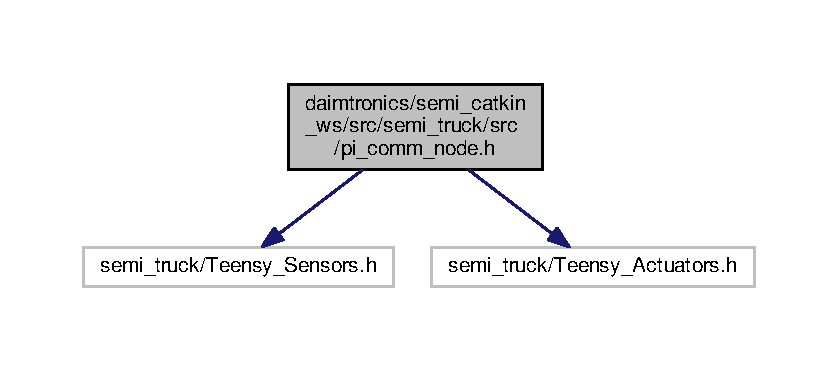
\includegraphics[width=350pt]{pi__comm__node_8h__incl}
\end{center}
\end{figure}
This graph shows which files directly or indirectly include this file\+:
\nopagebreak
\begin{figure}[H]
\begin{center}
\leavevmode
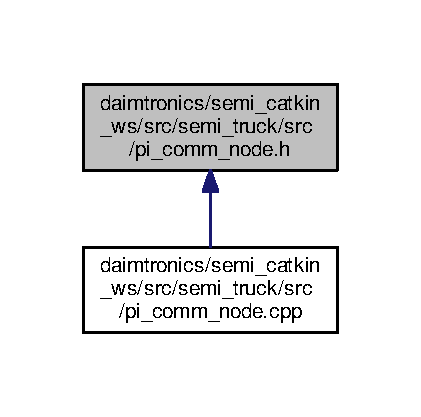
\includegraphics[width=202pt]{pi__comm__node_8h__dep__incl}
\end{center}
\end{figure}
\subsection*{Functions}
\begin{DoxyCompactItemize}
\item 
short \hyperlink{pi__comm__node_8h_a41b126a0cd4632cb40a651336b009cf5}{read\+\_\+sensor\+\_\+msg} (int serial, char num\+\_\+bytes)
\begin{DoxyCompactList}\small\item\em Reads a single value from the U\+A\+RT communication buffer. \end{DoxyCompactList}\item 
void \hyperlink{pi__comm__node_8h_a0c5cd860a6d8f747aea77d78d2e8bb7c}{read\+\_\+from\+\_\+teensy} (int serial, \hyperlink{namespacesemi__truck_a8ffe15bf9a1e739c2242ac6d6feaa67f}{semi\+\_\+truck\+::\+Teensy\+\_\+\+Sensors} \&sensors)
\begin{DoxyCompactList}\small\item\em Reads an entire set of Teensy sensor data by calling read\+\_\+sensor\+\_\+msg on each sensor data in the U\+A\+RT message. \end{DoxyCompactList}\item 
void \hyperlink{pi__comm__node_8h_ab7163db1bba4dc09fdd91cf80de4eefc}{write\+\_\+sensor\+\_\+msg} (int serial, short sensor\+\_\+val, char num\+\_\+bytes)
\item 
void \hyperlink{pi__comm__node_8h_af969dff0aa66a4e3c813f09b452050cc}{write\+\_\+to\+\_\+teensy} (int serial, const \hyperlink{namespacesemi__truck_ab8254dd176d8fef1f1381fb4e7e5e869}{semi\+\_\+truck\+::\+Teensy\+\_\+\+Actuators} \&actuators)
\begin{DoxyCompactList}\small\item\em Writes an entire set of actuator data to the Teensy via U\+A\+RT. \end{DoxyCompactList}\item 
void \hyperlink{pi__comm__node_8h_af5ff714d028d70416196bba7c64c5da7}{update\+\_\+sensors} (\hyperlink{namespacesemi__truck_a8ffe15bf9a1e739c2242ac6d6feaa67f}{semi\+\_\+truck\+::\+Teensy\+\_\+\+Sensors} \&sensors)
\item 
void \hyperlink{pi__comm__node_8h_a1c868413212badac680da7f573eb6be4}{pi\+\_\+sync} ()
\begin{DoxyCompactList}\small\item\em Called before reading sensor data from the Teensy. It will read the buffer until it encounters the S\+Y\+N\+C\+\_\+\+V\+A\+L\+UE that has been defined. Once this happens, the next set of bytes are the set of sensor values. \end{DoxyCompactList}\item 
void \hyperlink{pi__comm__node_8h_a25959d1c80ccb8a385982b0cec8750fb}{print\+\_\+sensors} (const \hyperlink{namespacesemi__truck_a8ffe15bf9a1e739c2242ac6d6feaa67f}{semi\+\_\+truck\+::\+Teensy\+\_\+\+Sensors} \&sensors)
\begin{DoxyCompactList}\small\item\em A function useful for debugging serial communication. Prints the entire set of sensor data to the console. \end{DoxyCompactList}\item 
void \hyperlink{pi__comm__node_8h_ae1e75fea7e23242bb9d5d43771a2765a}{print\+\_\+actuators} (const \hyperlink{namespacesemi__truck_ab8254dd176d8fef1f1381fb4e7e5e869}{semi\+\_\+truck\+::\+Teensy\+\_\+\+Actuators} \&actuators)
\begin{DoxyCompactList}\small\item\em A function useful for debugging serial communication. Prints the entire set of actuator data to the console. \end{DoxyCompactList}\item 
void \hyperlink{pi__comm__node_8h_a6f2420fd51a76bb6a8a5e5970a7a6f27}{sensor\+\_\+cb} (const \hyperlink{namespacesemi__truck_a8ffe15bf9a1e739c2242ac6d6feaa67f}{semi\+\_\+truck\+::\+Teensy\+\_\+\+Sensors} \&msg)
\item 
void \hyperlink{pi__comm__node_8h_a12284c231750c1247c39d646e6c26f80}{actuator\+\_\+cb} (const \hyperlink{namespacesemi__truck_ab8254dd176d8fef1f1381fb4e7e5e869}{semi\+\_\+truck\+::\+Teensy\+\_\+\+Actuators} \&msg)
\begin{DoxyCompactList}\small\item\em The callback function the the subscriber to the teensy\+\_\+actuator\+\_\+data topic. This function will run every time R\+O\+S\+::spin\+Once is called. It reads the set of data from the topic and immediately writes these values to the Teensy via U\+A\+RT. \end{DoxyCompactList}\end{DoxyCompactItemize}


\subsection{Function Documentation}
\index{pi\+\_\+comm\+\_\+node.\+h@{pi\+\_\+comm\+\_\+node.\+h}!actuator\+\_\+cb@{actuator\+\_\+cb}}
\index{actuator\+\_\+cb@{actuator\+\_\+cb}!pi\+\_\+comm\+\_\+node.\+h@{pi\+\_\+comm\+\_\+node.\+h}}
\subsubsection[{\texorpdfstring{actuator\+\_\+cb(const semi\+\_\+truck\+::\+Teensy\+\_\+\+Actuators \&msg)}{actuator_cb(const semi_truck::Teensy_Actuators &msg)}}]{\setlength{\rightskip}{0pt plus 5cm}void actuator\+\_\+cb (
\begin{DoxyParamCaption}
\item[{const {\bf semi\+\_\+truck\+::\+Teensy\+\_\+\+Actuators} \&}]{msg}
\end{DoxyParamCaption}
)}\hypertarget{pi__comm__node_8h_a12284c231750c1247c39d646e6c26f80}{}\label{pi__comm__node_8h_a12284c231750c1247c39d646e6c26f80}


The callback function the the subscriber to the teensy\+\_\+actuator\+\_\+data topic. This function will run every time R\+O\+S\+::spin\+Once is called. It reads the set of data from the topic and immediately writes these values to the Teensy via U\+A\+RT. 


\begin{DoxyParams}{Parameters}
{\em msg} & A set of actuator data that has come from the actuator topic and needs to be written to the Teensy. \\
\hline
\end{DoxyParams}
\index{pi\+\_\+comm\+\_\+node.\+h@{pi\+\_\+comm\+\_\+node.\+h}!pi\+\_\+sync@{pi\+\_\+sync}}
\index{pi\+\_\+sync@{pi\+\_\+sync}!pi\+\_\+comm\+\_\+node.\+h@{pi\+\_\+comm\+\_\+node.\+h}}
\subsubsection[{\texorpdfstring{pi\+\_\+sync()}{pi_sync()}}]{\setlength{\rightskip}{0pt plus 5cm}void pi\+\_\+sync (
\begin{DoxyParamCaption}
{}
\end{DoxyParamCaption}
)}\hypertarget{pi__comm__node_8h_a1c868413212badac680da7f573eb6be4}{}\label{pi__comm__node_8h_a1c868413212badac680da7f573eb6be4}


Called before reading sensor data from the Teensy. It will read the buffer until it encounters the S\+Y\+N\+C\+\_\+\+V\+A\+L\+UE that has been defined. Once this happens, the next set of bytes are the set of sensor values. 

\index{pi\+\_\+comm\+\_\+node.\+h@{pi\+\_\+comm\+\_\+node.\+h}!print\+\_\+actuators@{print\+\_\+actuators}}
\index{print\+\_\+actuators@{print\+\_\+actuators}!pi\+\_\+comm\+\_\+node.\+h@{pi\+\_\+comm\+\_\+node.\+h}}
\subsubsection[{\texorpdfstring{print\+\_\+actuators(const semi\+\_\+truck\+::\+Teensy\+\_\+\+Actuators \&actuators)}{print_actuators(const semi_truck::Teensy_Actuators &actuators)}}]{\setlength{\rightskip}{0pt plus 5cm}void print\+\_\+actuators (
\begin{DoxyParamCaption}
\item[{const {\bf semi\+\_\+truck\+::\+Teensy\+\_\+\+Actuators} \&}]{actuators}
\end{DoxyParamCaption}
)}\hypertarget{pi__comm__node_8h_ae1e75fea7e23242bb9d5d43771a2765a}{}\label{pi__comm__node_8h_ae1e75fea7e23242bb9d5d43771a2765a}


A function useful for debugging serial communication. Prints the entire set of actuator data to the console. 


\begin{DoxyParams}{Parameters}
{\em actuators} & The object that holds all of the actuator data \\
\hline
\end{DoxyParams}
\index{pi\+\_\+comm\+\_\+node.\+h@{pi\+\_\+comm\+\_\+node.\+h}!print\+\_\+sensors@{print\+\_\+sensors}}
\index{print\+\_\+sensors@{print\+\_\+sensors}!pi\+\_\+comm\+\_\+node.\+h@{pi\+\_\+comm\+\_\+node.\+h}}
\subsubsection[{\texorpdfstring{print\+\_\+sensors(const semi\+\_\+truck\+::\+Teensy\+\_\+\+Sensors \&sensors)}{print_sensors(const semi_truck::Teensy_Sensors &sensors)}}]{\setlength{\rightskip}{0pt plus 5cm}void print\+\_\+sensors (
\begin{DoxyParamCaption}
\item[{const {\bf semi\+\_\+truck\+::\+Teensy\+\_\+\+Sensors} \&}]{sensors}
\end{DoxyParamCaption}
)}\hypertarget{pi__comm__node_8h_a25959d1c80ccb8a385982b0cec8750fb}{}\label{pi__comm__node_8h_a25959d1c80ccb8a385982b0cec8750fb}


A function useful for debugging serial communication. Prints the entire set of sensor data to the console. 


\begin{DoxyParams}{Parameters}
{\em sensors} & The object that holds all of the sensor data \\
\hline
\end{DoxyParams}
\index{pi\+\_\+comm\+\_\+node.\+h@{pi\+\_\+comm\+\_\+node.\+h}!read\+\_\+from\+\_\+teensy@{read\+\_\+from\+\_\+teensy}}
\index{read\+\_\+from\+\_\+teensy@{read\+\_\+from\+\_\+teensy}!pi\+\_\+comm\+\_\+node.\+h@{pi\+\_\+comm\+\_\+node.\+h}}
\subsubsection[{\texorpdfstring{read\+\_\+from\+\_\+teensy(int serial, semi\+\_\+truck\+::\+Teensy\+\_\+\+Sensors \&sensors)}{read_from_teensy(int serial, semi_truck::Teensy_Sensors &sensors)}}]{\setlength{\rightskip}{0pt plus 5cm}void read\+\_\+from\+\_\+teensy (
\begin{DoxyParamCaption}
\item[{int}]{serial, }
\item[{{\bf semi\+\_\+truck\+::\+Teensy\+\_\+\+Sensors} \&}]{sensors}
\end{DoxyParamCaption}
)}\hypertarget{pi__comm__node_8h_a0c5cd860a6d8f747aea77d78d2e8bb7c}{}\label{pi__comm__node_8h_a0c5cd860a6d8f747aea77d78d2e8bb7c}


Reads an entire set of Teensy sensor data by calling read\+\_\+sensor\+\_\+msg on each sensor data in the U\+A\+RT message. 

\index{pi\+\_\+comm\+\_\+node.\+h@{pi\+\_\+comm\+\_\+node.\+h}!read\+\_\+sensor\+\_\+msg@{read\+\_\+sensor\+\_\+msg}}
\index{read\+\_\+sensor\+\_\+msg@{read\+\_\+sensor\+\_\+msg}!pi\+\_\+comm\+\_\+node.\+h@{pi\+\_\+comm\+\_\+node.\+h}}
\subsubsection[{\texorpdfstring{read\+\_\+sensor\+\_\+msg(int serial, char num\+\_\+bytes)}{read_sensor_msg(int serial, char num_bytes)}}]{\setlength{\rightskip}{0pt plus 5cm}short read\+\_\+sensor\+\_\+msg (
\begin{DoxyParamCaption}
\item[{int}]{serial, }
\item[{char}]{num\+\_\+bytes}
\end{DoxyParamCaption}
)}\hypertarget{pi__comm__node_8h_a41b126a0cd4632cb40a651336b009cf5}{}\label{pi__comm__node_8h_a41b126a0cd4632cb40a651336b009cf5}


Reads a single value from the U\+A\+RT communication buffer. 


\begin{DoxyParams}{Parameters}
{\em serial} & The serial file descriptor to read from \\
\hline
{\em num\+\_\+bytes} & The number of bytes to read from \\
\hline
\end{DoxyParams}
\begin{DoxyReturn}{Returns}
The value of the bytes that have been read 
\end{DoxyReturn}
\index{pi\+\_\+comm\+\_\+node.\+h@{pi\+\_\+comm\+\_\+node.\+h}!sensor\+\_\+cb@{sensor\+\_\+cb}}
\index{sensor\+\_\+cb@{sensor\+\_\+cb}!pi\+\_\+comm\+\_\+node.\+h@{pi\+\_\+comm\+\_\+node.\+h}}
\subsubsection[{\texorpdfstring{sensor\+\_\+cb(const semi\+\_\+truck\+::\+Teensy\+\_\+\+Sensors \&msg)}{sensor_cb(const semi_truck::Teensy_Sensors &msg)}}]{\setlength{\rightskip}{0pt plus 5cm}void sensor\+\_\+cb (
\begin{DoxyParamCaption}
\item[{const {\bf semi\+\_\+truck\+::\+Teensy\+\_\+\+Sensors} \&}]{msg}
\end{DoxyParamCaption}
)}\hypertarget{pi__comm__node_8h_a6f2420fd51a76bb6a8a5e5970a7a6f27}{}\label{pi__comm__node_8h_a6f2420fd51a76bb6a8a5e5970a7a6f27}
\index{pi\+\_\+comm\+\_\+node.\+h@{pi\+\_\+comm\+\_\+node.\+h}!update\+\_\+sensors@{update\+\_\+sensors}}
\index{update\+\_\+sensors@{update\+\_\+sensors}!pi\+\_\+comm\+\_\+node.\+h@{pi\+\_\+comm\+\_\+node.\+h}}
\subsubsection[{\texorpdfstring{update\+\_\+sensors(semi\+\_\+truck\+::\+Teensy\+\_\+\+Sensors \&sensors)}{update_sensors(semi_truck::Teensy_Sensors &sensors)}}]{\setlength{\rightskip}{0pt plus 5cm}void update\+\_\+sensors (
\begin{DoxyParamCaption}
\item[{{\bf semi\+\_\+truck\+::\+Teensy\+\_\+\+Sensors} \&}]{sensors}
\end{DoxyParamCaption}
)}\hypertarget{pi__comm__node_8h_af5ff714d028d70416196bba7c64c5da7}{}\label{pi__comm__node_8h_af5ff714d028d70416196bba7c64c5da7}
\index{pi\+\_\+comm\+\_\+node.\+h@{pi\+\_\+comm\+\_\+node.\+h}!write\+\_\+sensor\+\_\+msg@{write\+\_\+sensor\+\_\+msg}}
\index{write\+\_\+sensor\+\_\+msg@{write\+\_\+sensor\+\_\+msg}!pi\+\_\+comm\+\_\+node.\+h@{pi\+\_\+comm\+\_\+node.\+h}}
\subsubsection[{\texorpdfstring{write\+\_\+sensor\+\_\+msg(int serial, short sensor\+\_\+val, char num\+\_\+bytes)}{write_sensor_msg(int serial, short sensor_val, char num_bytes)}}]{\setlength{\rightskip}{0pt plus 5cm}void write\+\_\+sensor\+\_\+msg (
\begin{DoxyParamCaption}
\item[{int}]{serial, }
\item[{short}]{sensor\+\_\+val, }
\item[{char}]{num\+\_\+bytes}
\end{DoxyParamCaption}
)}\hypertarget{pi__comm__node_8h_ab7163db1bba4dc09fdd91cf80de4eefc}{}\label{pi__comm__node_8h_ab7163db1bba4dc09fdd91cf80de4eefc}
\index{pi\+\_\+comm\+\_\+node.\+h@{pi\+\_\+comm\+\_\+node.\+h}!write\+\_\+to\+\_\+teensy@{write\+\_\+to\+\_\+teensy}}
\index{write\+\_\+to\+\_\+teensy@{write\+\_\+to\+\_\+teensy}!pi\+\_\+comm\+\_\+node.\+h@{pi\+\_\+comm\+\_\+node.\+h}}
\subsubsection[{\texorpdfstring{write\+\_\+to\+\_\+teensy(int serial, const semi\+\_\+truck\+::\+Teensy\+\_\+\+Actuators \&actuators)}{write_to_teensy(int serial, const semi_truck::Teensy_Actuators &actuators)}}]{\setlength{\rightskip}{0pt plus 5cm}void write\+\_\+to\+\_\+teensy (
\begin{DoxyParamCaption}
\item[{int}]{serial, }
\item[{const {\bf semi\+\_\+truck\+::\+Teensy\+\_\+\+Actuators} \&}]{actuators}
\end{DoxyParamCaption}
)}\hypertarget{pi__comm__node_8h_af969dff0aa66a4e3c813f09b452050cc}{}\label{pi__comm__node_8h_af969dff0aa66a4e3c813f09b452050cc}


Writes an entire set of actuator data to the Teensy via U\+A\+RT. 


\begin{DoxyParams}{Parameters}
{\em serial} & The serial file descriptor to write to \\
\hline
{\em actuators} & The object that holds all of the actuator data \\
\hline
\end{DoxyParams}

\hypertarget{semi__truck__api_8cpp}{}\section{daimtronics/semi\+\_\+catkin\+\_\+ws/src/semi\+\_\+truck/src/semi\+\_\+truck\+\_\+api.cpp File Reference}
\label{semi__truck__api_8cpp}\index{daimtronics/semi\+\_\+catkin\+\_\+ws/src/semi\+\_\+truck/src/semi\+\_\+truck\+\_\+api.\+cpp@{daimtronics/semi\+\_\+catkin\+\_\+ws/src/semi\+\_\+truck/src/semi\+\_\+truck\+\_\+api.\+cpp}}
{\ttfamily \#include \char`\"{}semi\+\_\+truck\+\_\+api.\+h\char`\"{}}\\*
Include dependency graph for semi\+\_\+truck\+\_\+api.\+cpp\+:
\nopagebreak
\begin{figure}[H]
\begin{center}
\leavevmode
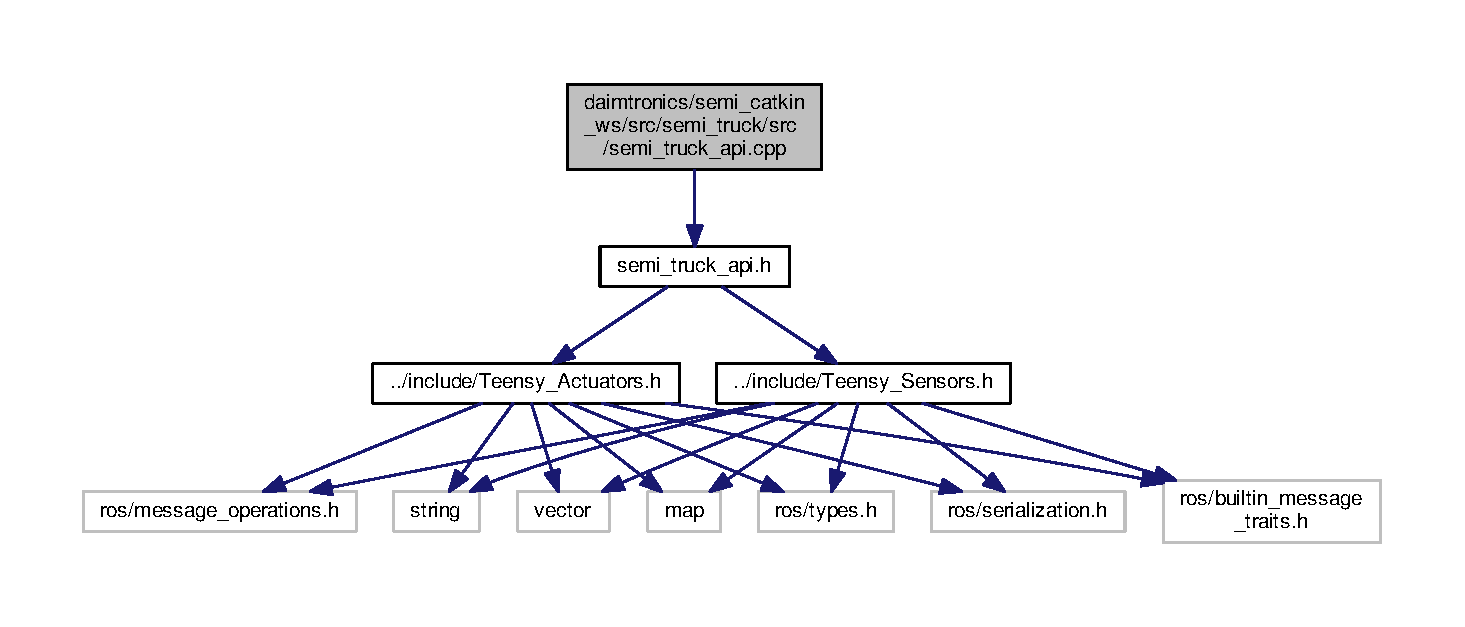
\includegraphics[width=350pt]{semi__truck__api_8cpp__incl}
\end{center}
\end{figure}
\subsection*{Functions}
\begin{DoxyCompactItemize}
\item 
void \hyperlink{semi__truck__api_8cpp_a7a87c514f6941b049d0682587bf79a19}{set\+\_\+motor\+\_\+output} (\hyperlink{namespacesemi__truck_ab8254dd176d8fef1f1381fb4e7e5e869}{semi\+\_\+truck\+::\+Teensy\+\_\+\+Actuators} \&actuators, int16\+\_\+t motor\+\_\+output)
\begin{DoxyCompactList}\small\item\em sets the motor output of the actuators object to the passed in value \end{DoxyCompactList}\item 
void \hyperlink{semi__truck__api_8cpp_a4ae9e9386bbc2f69a7e5aad0ade8ce3a}{set\+\_\+steer\+\_\+output} (\hyperlink{namespacesemi__truck_ab8254dd176d8fef1f1381fb4e7e5e869}{semi\+\_\+truck\+::\+Teensy\+\_\+\+Actuators} \&actuators, int16\+\_\+t steer\+\_\+output)
\begin{DoxyCompactList}\small\item\em sets the steer output of the actuators object to the passed in value \end{DoxyCompactList}\item 
void \hyperlink{semi__truck__api_8cpp_aca24955ade43b742a379835b9e085bfd}{set\+\_\+fifth\+\_\+output} (\hyperlink{namespacesemi__truck_ab8254dd176d8fef1f1381fb4e7e5e869}{semi\+\_\+truck\+::\+Teensy\+\_\+\+Actuators} \&actuators, uint16\+\_\+t fifth\+\_\+output)
\begin{DoxyCompactList}\small\item\em sets the fifth wheel of the actuators object to the passed in value \end{DoxyCompactList}\item 
int16\+\_\+t \hyperlink{semi__truck__api_8cpp_a9102242c618a806b37b29e8cf755635a}{get\+\_\+wheel\+\_\+speed} (\hyperlink{namespacesemi__truck_a8ffe15bf9a1e739c2242ac6d6feaa67f}{semi\+\_\+truck\+::\+Teensy\+\_\+\+Sensors} \&sensors)
\begin{DoxyCompactList}\small\item\em reads the wheel speed of a Teensy\+Sensors object \end{DoxyCompactList}\item 
int16\+\_\+t \hyperlink{semi__truck__api_8cpp_ad2a88a4acb04875ce8af7529b8c134aa}{get\+\_\+imu\+\_\+angle} (\hyperlink{namespacesemi__truck_a8ffe15bf9a1e739c2242ac6d6feaa67f}{semi\+\_\+truck\+::\+Teensy\+\_\+\+Sensors} \&sensors)
\begin{DoxyCompactList}\small\item\em reads the imu angle (degrees) of a Teensy\+Sensors object \end{DoxyCompactList}\item 
int16\+\_\+t \hyperlink{semi__truck__api_8cpp_a49c1affdb96da8177f02ede6de778ac1}{get\+\_\+right\+\_\+\+T\+OF} (\hyperlink{namespacesemi__truck_a8ffe15bf9a1e739c2242ac6d6feaa67f}{semi\+\_\+truck\+::\+Teensy\+\_\+\+Sensors} \&sensors)
\begin{DoxyCompactList}\small\item\em reads the right T\+OF distance (cm) of a Teensy\+Sensors object \end{DoxyCompactList}\item 
int16\+\_\+t \hyperlink{semi__truck__api_8cpp_ae911633732f68cbf43db9ffcf06a0a41}{get\+\_\+left\+\_\+\+T\+OF} (\hyperlink{namespacesemi__truck_a8ffe15bf9a1e739c2242ac6d6feaa67f}{semi\+\_\+truck\+::\+Teensy\+\_\+\+Sensors} \&sensors)
\begin{DoxyCompactList}\small\item\em reads the left T\+OF distance (cm) of a Teensy\+Sensors object \end{DoxyCompactList}\item 
int16\+\_\+t \hyperlink{semi__truck__api_8cpp_a484706f88567e5def2555a03f69982ee}{get\+\_\+rear\+\_\+\+T\+OF} (\hyperlink{namespacesemi__truck_a8ffe15bf9a1e739c2242ac6d6feaa67f}{semi\+\_\+truck\+::\+Teensy\+\_\+\+Sensors} \&sensors)
\begin{DoxyCompactList}\small\item\em reads the rear T\+OF distance (cm) of a Teensy\+Sensors object \end{DoxyCompactList}\end{DoxyCompactItemize}


\subsection{Function Documentation}
\index{semi\+\_\+truck\+\_\+api.\+cpp@{semi\+\_\+truck\+\_\+api.\+cpp}!get\+\_\+imu\+\_\+angle@{get\+\_\+imu\+\_\+angle}}
\index{get\+\_\+imu\+\_\+angle@{get\+\_\+imu\+\_\+angle}!semi\+\_\+truck\+\_\+api.\+cpp@{semi\+\_\+truck\+\_\+api.\+cpp}}
\subsubsection[{\texorpdfstring{get\+\_\+imu\+\_\+angle(semi\+\_\+truck\+::\+Teensy\+\_\+\+Sensors \&sensors)}{get_imu_angle(semi_truck::Teensy_Sensors &sensors)}}]{\setlength{\rightskip}{0pt plus 5cm}int16\+\_\+t get\+\_\+imu\+\_\+angle (
\begin{DoxyParamCaption}
\item[{{\bf semi\+\_\+truck\+::\+Teensy\+\_\+\+Sensors} \&}]{sensors}
\end{DoxyParamCaption}
)}\hypertarget{semi__truck__api_8cpp_ad2a88a4acb04875ce8af7529b8c134aa}{}\label{semi__truck__api_8cpp_ad2a88a4acb04875ce8af7529b8c134aa}


reads the imu angle (degrees) of a Teensy\+Sensors object 


\begin{DoxyParams}{Parameters}
{\em sensors} & a reference to a Teensy\+Sensors object to read from. \\
\hline
\end{DoxyParams}
\index{semi\+\_\+truck\+\_\+api.\+cpp@{semi\+\_\+truck\+\_\+api.\+cpp}!get\+\_\+left\+\_\+\+T\+OF@{get\+\_\+left\+\_\+\+T\+OF}}
\index{get\+\_\+left\+\_\+\+T\+OF@{get\+\_\+left\+\_\+\+T\+OF}!semi\+\_\+truck\+\_\+api.\+cpp@{semi\+\_\+truck\+\_\+api.\+cpp}}
\subsubsection[{\texorpdfstring{get\+\_\+left\+\_\+\+T\+O\+F(semi\+\_\+truck\+::\+Teensy\+\_\+\+Sensors \&sensors)}{get_left_TOF(semi_truck::Teensy_Sensors &sensors)}}]{\setlength{\rightskip}{0pt plus 5cm}int16\+\_\+t get\+\_\+left\+\_\+\+T\+OF (
\begin{DoxyParamCaption}
\item[{{\bf semi\+\_\+truck\+::\+Teensy\+\_\+\+Sensors} \&}]{sensors}
\end{DoxyParamCaption}
)}\hypertarget{semi__truck__api_8cpp_ae911633732f68cbf43db9ffcf06a0a41}{}\label{semi__truck__api_8cpp_ae911633732f68cbf43db9ffcf06a0a41}


reads the left T\+OF distance (cm) of a Teensy\+Sensors object 


\begin{DoxyParams}{Parameters}
{\em sensors} & a reference to a Teensy\+Sensors object to read from. \\
\hline
\end{DoxyParams}
\index{semi\+\_\+truck\+\_\+api.\+cpp@{semi\+\_\+truck\+\_\+api.\+cpp}!get\+\_\+rear\+\_\+\+T\+OF@{get\+\_\+rear\+\_\+\+T\+OF}}
\index{get\+\_\+rear\+\_\+\+T\+OF@{get\+\_\+rear\+\_\+\+T\+OF}!semi\+\_\+truck\+\_\+api.\+cpp@{semi\+\_\+truck\+\_\+api.\+cpp}}
\subsubsection[{\texorpdfstring{get\+\_\+rear\+\_\+\+T\+O\+F(semi\+\_\+truck\+::\+Teensy\+\_\+\+Sensors \&sensors)}{get_rear_TOF(semi_truck::Teensy_Sensors &sensors)}}]{\setlength{\rightskip}{0pt plus 5cm}int16\+\_\+t get\+\_\+rear\+\_\+\+T\+OF (
\begin{DoxyParamCaption}
\item[{{\bf semi\+\_\+truck\+::\+Teensy\+\_\+\+Sensors} \&}]{sensors}
\end{DoxyParamCaption}
)}\hypertarget{semi__truck__api_8cpp_a484706f88567e5def2555a03f69982ee}{}\label{semi__truck__api_8cpp_a484706f88567e5def2555a03f69982ee}


reads the rear T\+OF distance (cm) of a Teensy\+Sensors object 


\begin{DoxyParams}{Parameters}
{\em sensors} & a reference to a Teensy\+Sensors object to read from. \\
\hline
\end{DoxyParams}
\index{semi\+\_\+truck\+\_\+api.\+cpp@{semi\+\_\+truck\+\_\+api.\+cpp}!get\+\_\+right\+\_\+\+T\+OF@{get\+\_\+right\+\_\+\+T\+OF}}
\index{get\+\_\+right\+\_\+\+T\+OF@{get\+\_\+right\+\_\+\+T\+OF}!semi\+\_\+truck\+\_\+api.\+cpp@{semi\+\_\+truck\+\_\+api.\+cpp}}
\subsubsection[{\texorpdfstring{get\+\_\+right\+\_\+\+T\+O\+F(semi\+\_\+truck\+::\+Teensy\+\_\+\+Sensors \&sensors)}{get_right_TOF(semi_truck::Teensy_Sensors &sensors)}}]{\setlength{\rightskip}{0pt plus 5cm}int16\+\_\+t get\+\_\+right\+\_\+\+T\+OF (
\begin{DoxyParamCaption}
\item[{{\bf semi\+\_\+truck\+::\+Teensy\+\_\+\+Sensors} \&}]{sensors}
\end{DoxyParamCaption}
)}\hypertarget{semi__truck__api_8cpp_a49c1affdb96da8177f02ede6de778ac1}{}\label{semi__truck__api_8cpp_a49c1affdb96da8177f02ede6de778ac1}


reads the right T\+OF distance (cm) of a Teensy\+Sensors object 


\begin{DoxyParams}{Parameters}
{\em sensors} & a reference to a Teensy\+Sensors object to read from. \\
\hline
\end{DoxyParams}
\index{semi\+\_\+truck\+\_\+api.\+cpp@{semi\+\_\+truck\+\_\+api.\+cpp}!get\+\_\+wheel\+\_\+speed@{get\+\_\+wheel\+\_\+speed}}
\index{get\+\_\+wheel\+\_\+speed@{get\+\_\+wheel\+\_\+speed}!semi\+\_\+truck\+\_\+api.\+cpp@{semi\+\_\+truck\+\_\+api.\+cpp}}
\subsubsection[{\texorpdfstring{get\+\_\+wheel\+\_\+speed(semi\+\_\+truck\+::\+Teensy\+\_\+\+Sensors \&sensors)}{get_wheel_speed(semi_truck::Teensy_Sensors &sensors)}}]{\setlength{\rightskip}{0pt plus 5cm}int16\+\_\+t get\+\_\+wheel\+\_\+speed (
\begin{DoxyParamCaption}
\item[{{\bf semi\+\_\+truck\+::\+Teensy\+\_\+\+Sensors} \&}]{sensors}
\end{DoxyParamCaption}
)}\hypertarget{semi__truck__api_8cpp_a9102242c618a806b37b29e8cf755635a}{}\label{semi__truck__api_8cpp_a9102242c618a806b37b29e8cf755635a}


reads the wheel speed of a Teensy\+Sensors object 


\begin{DoxyParams}{Parameters}
{\em sensors} & a reference to a Teensy\+Sensors object to read from. \\
\hline
\end{DoxyParams}
\index{semi\+\_\+truck\+\_\+api.\+cpp@{semi\+\_\+truck\+\_\+api.\+cpp}!set\+\_\+fifth\+\_\+output@{set\+\_\+fifth\+\_\+output}}
\index{set\+\_\+fifth\+\_\+output@{set\+\_\+fifth\+\_\+output}!semi\+\_\+truck\+\_\+api.\+cpp@{semi\+\_\+truck\+\_\+api.\+cpp}}
\subsubsection[{\texorpdfstring{set\+\_\+fifth\+\_\+output(semi\+\_\+truck\+::\+Teensy\+\_\+\+Actuators \&actuators, uint16\+\_\+t fifth\+\_\+output)}{set_fifth_output(semi_truck::Teensy_Actuators &actuators, uint16_t fifth_output)}}]{\setlength{\rightskip}{0pt plus 5cm}void set\+\_\+fifth\+\_\+output (
\begin{DoxyParamCaption}
\item[{{\bf semi\+\_\+truck\+::\+Teensy\+\_\+\+Actuators} \&}]{actuators, }
\item[{uint16\+\_\+t}]{value}
\end{DoxyParamCaption}
)}\hypertarget{semi__truck__api_8cpp_aca24955ade43b742a379835b9e085bfd}{}\label{semi__truck__api_8cpp_aca24955ade43b742a379835b9e085bfd}


sets the fifth wheel of the actuators object to the passed in value 


\begin{DoxyParams}{Parameters}
{\em actuators} & a reference to a Teensy\+Actuators object to alter \\
\hline
{\em value} & the value to update the actuators with. 0 for locked and 1 for unlocked. \\
\hline
\end{DoxyParams}
\index{semi\+\_\+truck\+\_\+api.\+cpp@{semi\+\_\+truck\+\_\+api.\+cpp}!set\+\_\+motor\+\_\+output@{set\+\_\+motor\+\_\+output}}
\index{set\+\_\+motor\+\_\+output@{set\+\_\+motor\+\_\+output}!semi\+\_\+truck\+\_\+api.\+cpp@{semi\+\_\+truck\+\_\+api.\+cpp}}
\subsubsection[{\texorpdfstring{set\+\_\+motor\+\_\+output(semi\+\_\+truck\+::\+Teensy\+\_\+\+Actuators \&actuators, int16\+\_\+t motor\+\_\+output)}{set_motor_output(semi_truck::Teensy_Actuators &actuators, int16_t motor_output)}}]{\setlength{\rightskip}{0pt plus 5cm}void set\+\_\+motor\+\_\+output (
\begin{DoxyParamCaption}
\item[{{\bf semi\+\_\+truck\+::\+Teensy\+\_\+\+Actuators} \&}]{actuators, }
\item[{int16\+\_\+t}]{value}
\end{DoxyParamCaption}
)}\hypertarget{semi__truck__api_8cpp_a7a87c514f6941b049d0682587bf79a19}{}\label{semi__truck__api_8cpp_a7a87c514f6941b049d0682587bf79a19}


sets the motor output of the actuators object to the passed in value 


\begin{DoxyParams}{Parameters}
{\em actuators} & a reference to a Teensy\+Actuators object to alter \\
\hline
{\em value} & the value to update the actuators with. This value should range from 0 for full reverse power to 180 for full forwards power. \\
\hline
\end{DoxyParams}
\index{semi\+\_\+truck\+\_\+api.\+cpp@{semi\+\_\+truck\+\_\+api.\+cpp}!set\+\_\+steer\+\_\+output@{set\+\_\+steer\+\_\+output}}
\index{set\+\_\+steer\+\_\+output@{set\+\_\+steer\+\_\+output}!semi\+\_\+truck\+\_\+api.\+cpp@{semi\+\_\+truck\+\_\+api.\+cpp}}
\subsubsection[{\texorpdfstring{set\+\_\+steer\+\_\+output(semi\+\_\+truck\+::\+Teensy\+\_\+\+Actuators \&actuators, int16\+\_\+t steer\+\_\+output)}{set_steer_output(semi_truck::Teensy_Actuators &actuators, int16_t steer_output)}}]{\setlength{\rightskip}{0pt plus 5cm}void set\+\_\+steer\+\_\+output (
\begin{DoxyParamCaption}
\item[{{\bf semi\+\_\+truck\+::\+Teensy\+\_\+\+Actuators} \&}]{actuators, }
\item[{int16\+\_\+t}]{value}
\end{DoxyParamCaption}
)}\hypertarget{semi__truck__api_8cpp_a4ae9e9386bbc2f69a7e5aad0ade8ce3a}{}\label{semi__truck__api_8cpp_a4ae9e9386bbc2f69a7e5aad0ade8ce3a}


sets the steer output of the actuators object to the passed in value 


\begin{DoxyParams}{Parameters}
{\em actuators} & a reference to a Teensy\+Actuators object to alter \\
\hline
{\em value} & the value to update the actuators with. This value should range from 0 for a 20 degree angle left to 180 for a 20 degree angle right. \\
\hline
\end{DoxyParams}

\hypertarget{semi__truck__api_8h}{}\section{daimtronics/semi\+\_\+catkin\+\_\+ws/src/semi\+\_\+truck/src/semi\+\_\+truck\+\_\+api.h File Reference}
\label{semi__truck__api_8h}\index{daimtronics/semi\+\_\+catkin\+\_\+ws/src/semi\+\_\+truck/src/semi\+\_\+truck\+\_\+api.\+h@{daimtronics/semi\+\_\+catkin\+\_\+ws/src/semi\+\_\+truck/src/semi\+\_\+truck\+\_\+api.\+h}}
{\ttfamily \#include \char`\"{}../include/\+Teensy\+\_\+\+Actuators.\+h\char`\"{}}\\*
{\ttfamily \#include \char`\"{}../include/\+Teensy\+\_\+\+Sensors.\+h\char`\"{}}\\*
Include dependency graph for semi\+\_\+truck\+\_\+api.\+h\+:
\nopagebreak
\begin{figure}[H]
\begin{center}
\leavevmode
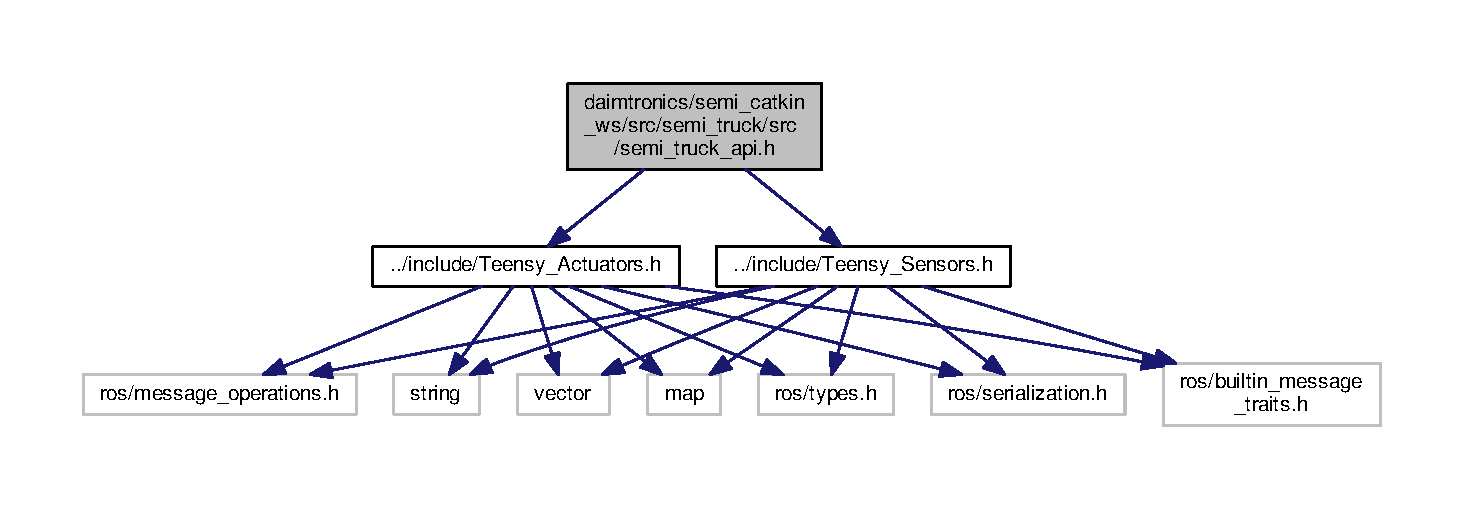
\includegraphics[width=350pt]{semi__truck__api_8h__incl}
\end{center}
\end{figure}
This graph shows which files directly or indirectly include this file\+:
\nopagebreak
\begin{figure}[H]
\begin{center}
\leavevmode
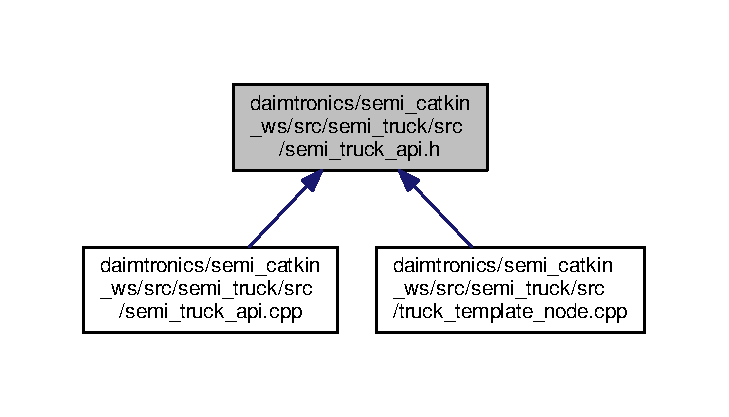
\includegraphics[width=350pt]{semi__truck__api_8h__dep__incl}
\end{center}
\end{figure}
\subsection*{Functions}
\begin{DoxyCompactItemize}
\item 
void \hyperlink{semi__truck__api_8h_ac2e5870ee4d48809b68d212bd3aeb6a1}{set\+\_\+motor\+\_\+output} (\hyperlink{namespacesemi__truck_ab8254dd176d8fef1f1381fb4e7e5e869}{semi\+\_\+truck\+::\+Teensy\+\_\+\+Actuators} \&actuators, int16\+\_\+t value)
\begin{DoxyCompactList}\small\item\em sets the motor output of the actuators object to the passed in value \end{DoxyCompactList}\item 
void \hyperlink{semi__truck__api_8h_aba42ffb6c28d49a879ea7ea82f2e7269}{set\+\_\+steer\+\_\+output} (\hyperlink{namespacesemi__truck_ab8254dd176d8fef1f1381fb4e7e5e869}{semi\+\_\+truck\+::\+Teensy\+\_\+\+Actuators} \&actuators, int16\+\_\+t value)
\begin{DoxyCompactList}\small\item\em sets the steer output of the actuators object to the passed in value \end{DoxyCompactList}\item 
void \hyperlink{semi__truck__api_8h_afef4485d3c5b0419e27f3dcac857fad9}{set\+\_\+fifth\+\_\+output} (\hyperlink{namespacesemi__truck_ab8254dd176d8fef1f1381fb4e7e5e869}{semi\+\_\+truck\+::\+Teensy\+\_\+\+Actuators} \&actuators, uint16\+\_\+t value)
\begin{DoxyCompactList}\small\item\em sets the fifth wheel of the actuators object to the passed in value \end{DoxyCompactList}\item 
int16\+\_\+t \hyperlink{semi__truck__api_8h_a9102242c618a806b37b29e8cf755635a}{get\+\_\+wheel\+\_\+speed} (\hyperlink{namespacesemi__truck_a8ffe15bf9a1e739c2242ac6d6feaa67f}{semi\+\_\+truck\+::\+Teensy\+\_\+\+Sensors} \&sensors)
\begin{DoxyCompactList}\small\item\em reads the wheel speed of a Teensy\+Sensors object \end{DoxyCompactList}\item 
int16\+\_\+t \hyperlink{semi__truck__api_8h_ad2a88a4acb04875ce8af7529b8c134aa}{get\+\_\+imu\+\_\+angle} (\hyperlink{namespacesemi__truck_a8ffe15bf9a1e739c2242ac6d6feaa67f}{semi\+\_\+truck\+::\+Teensy\+\_\+\+Sensors} \&sensors)
\begin{DoxyCompactList}\small\item\em reads the imu angle (degrees) of a Teensy\+Sensors object \end{DoxyCompactList}\item 
int16\+\_\+t \hyperlink{semi__truck__api_8h_a49c1affdb96da8177f02ede6de778ac1}{get\+\_\+right\+\_\+\+T\+OF} (\hyperlink{namespacesemi__truck_a8ffe15bf9a1e739c2242ac6d6feaa67f}{semi\+\_\+truck\+::\+Teensy\+\_\+\+Sensors} \&sensors)
\begin{DoxyCompactList}\small\item\em reads the right T\+OF distance (cm) of a Teensy\+Sensors object \end{DoxyCompactList}\item 
int16\+\_\+t \hyperlink{semi__truck__api_8h_ae911633732f68cbf43db9ffcf06a0a41}{get\+\_\+left\+\_\+\+T\+OF} (\hyperlink{namespacesemi__truck_a8ffe15bf9a1e739c2242ac6d6feaa67f}{semi\+\_\+truck\+::\+Teensy\+\_\+\+Sensors} \&sensors)
\begin{DoxyCompactList}\small\item\em reads the left T\+OF distance (cm) of a Teensy\+Sensors object \end{DoxyCompactList}\item 
int16\+\_\+t \hyperlink{semi__truck__api_8h_a484706f88567e5def2555a03f69982ee}{get\+\_\+rear\+\_\+\+T\+OF} (\hyperlink{namespacesemi__truck_a8ffe15bf9a1e739c2242ac6d6feaa67f}{semi\+\_\+truck\+::\+Teensy\+\_\+\+Sensors} \&sensors)
\begin{DoxyCompactList}\small\item\em reads the rear T\+OF distance (cm) of a Teensy\+Sensors object \end{DoxyCompactList}\end{DoxyCompactItemize}


\subsection{Function Documentation}
\index{semi\+\_\+truck\+\_\+api.\+h@{semi\+\_\+truck\+\_\+api.\+h}!get\+\_\+imu\+\_\+angle@{get\+\_\+imu\+\_\+angle}}
\index{get\+\_\+imu\+\_\+angle@{get\+\_\+imu\+\_\+angle}!semi\+\_\+truck\+\_\+api.\+h@{semi\+\_\+truck\+\_\+api.\+h}}
\subsubsection[{\texorpdfstring{get\+\_\+imu\+\_\+angle(semi\+\_\+truck\+::\+Teensy\+\_\+\+Sensors \&sensors)}{get_imu_angle(semi_truck::Teensy_Sensors &sensors)}}]{\setlength{\rightskip}{0pt plus 5cm}int16\+\_\+t get\+\_\+imu\+\_\+angle (
\begin{DoxyParamCaption}
\item[{{\bf semi\+\_\+truck\+::\+Teensy\+\_\+\+Sensors} \&}]{sensors}
\end{DoxyParamCaption}
)}\hypertarget{semi__truck__api_8h_ad2a88a4acb04875ce8af7529b8c134aa}{}\label{semi__truck__api_8h_ad2a88a4acb04875ce8af7529b8c134aa}


reads the imu angle (degrees) of a Teensy\+Sensors object 


\begin{DoxyParams}{Parameters}
{\em sensors} & a reference to a Teensy\+Sensors object to read from. \\
\hline
\end{DoxyParams}
\index{semi\+\_\+truck\+\_\+api.\+h@{semi\+\_\+truck\+\_\+api.\+h}!get\+\_\+left\+\_\+\+T\+OF@{get\+\_\+left\+\_\+\+T\+OF}}
\index{get\+\_\+left\+\_\+\+T\+OF@{get\+\_\+left\+\_\+\+T\+OF}!semi\+\_\+truck\+\_\+api.\+h@{semi\+\_\+truck\+\_\+api.\+h}}
\subsubsection[{\texorpdfstring{get\+\_\+left\+\_\+\+T\+O\+F(semi\+\_\+truck\+::\+Teensy\+\_\+\+Sensors \&sensors)}{get_left_TOF(semi_truck::Teensy_Sensors &sensors)}}]{\setlength{\rightskip}{0pt plus 5cm}int16\+\_\+t get\+\_\+left\+\_\+\+T\+OF (
\begin{DoxyParamCaption}
\item[{{\bf semi\+\_\+truck\+::\+Teensy\+\_\+\+Sensors} \&}]{sensors}
\end{DoxyParamCaption}
)}\hypertarget{semi__truck__api_8h_ae911633732f68cbf43db9ffcf06a0a41}{}\label{semi__truck__api_8h_ae911633732f68cbf43db9ffcf06a0a41}


reads the left T\+OF distance (cm) of a Teensy\+Sensors object 


\begin{DoxyParams}{Parameters}
{\em sensors} & a reference to a Teensy\+Sensors object to read from. \\
\hline
\end{DoxyParams}
\index{semi\+\_\+truck\+\_\+api.\+h@{semi\+\_\+truck\+\_\+api.\+h}!get\+\_\+rear\+\_\+\+T\+OF@{get\+\_\+rear\+\_\+\+T\+OF}}
\index{get\+\_\+rear\+\_\+\+T\+OF@{get\+\_\+rear\+\_\+\+T\+OF}!semi\+\_\+truck\+\_\+api.\+h@{semi\+\_\+truck\+\_\+api.\+h}}
\subsubsection[{\texorpdfstring{get\+\_\+rear\+\_\+\+T\+O\+F(semi\+\_\+truck\+::\+Teensy\+\_\+\+Sensors \&sensors)}{get_rear_TOF(semi_truck::Teensy_Sensors &sensors)}}]{\setlength{\rightskip}{0pt plus 5cm}int16\+\_\+t get\+\_\+rear\+\_\+\+T\+OF (
\begin{DoxyParamCaption}
\item[{{\bf semi\+\_\+truck\+::\+Teensy\+\_\+\+Sensors} \&}]{sensors}
\end{DoxyParamCaption}
)}\hypertarget{semi__truck__api_8h_a484706f88567e5def2555a03f69982ee}{}\label{semi__truck__api_8h_a484706f88567e5def2555a03f69982ee}


reads the rear T\+OF distance (cm) of a Teensy\+Sensors object 


\begin{DoxyParams}{Parameters}
{\em sensors} & a reference to a Teensy\+Sensors object to read from. \\
\hline
\end{DoxyParams}
\index{semi\+\_\+truck\+\_\+api.\+h@{semi\+\_\+truck\+\_\+api.\+h}!get\+\_\+right\+\_\+\+T\+OF@{get\+\_\+right\+\_\+\+T\+OF}}
\index{get\+\_\+right\+\_\+\+T\+OF@{get\+\_\+right\+\_\+\+T\+OF}!semi\+\_\+truck\+\_\+api.\+h@{semi\+\_\+truck\+\_\+api.\+h}}
\subsubsection[{\texorpdfstring{get\+\_\+right\+\_\+\+T\+O\+F(semi\+\_\+truck\+::\+Teensy\+\_\+\+Sensors \&sensors)}{get_right_TOF(semi_truck::Teensy_Sensors &sensors)}}]{\setlength{\rightskip}{0pt plus 5cm}int16\+\_\+t get\+\_\+right\+\_\+\+T\+OF (
\begin{DoxyParamCaption}
\item[{{\bf semi\+\_\+truck\+::\+Teensy\+\_\+\+Sensors} \&}]{sensors}
\end{DoxyParamCaption}
)}\hypertarget{semi__truck__api_8h_a49c1affdb96da8177f02ede6de778ac1}{}\label{semi__truck__api_8h_a49c1affdb96da8177f02ede6de778ac1}


reads the right T\+OF distance (cm) of a Teensy\+Sensors object 


\begin{DoxyParams}{Parameters}
{\em sensors} & a reference to a Teensy\+Sensors object to read from. \\
\hline
\end{DoxyParams}
\index{semi\+\_\+truck\+\_\+api.\+h@{semi\+\_\+truck\+\_\+api.\+h}!get\+\_\+wheel\+\_\+speed@{get\+\_\+wheel\+\_\+speed}}
\index{get\+\_\+wheel\+\_\+speed@{get\+\_\+wheel\+\_\+speed}!semi\+\_\+truck\+\_\+api.\+h@{semi\+\_\+truck\+\_\+api.\+h}}
\subsubsection[{\texorpdfstring{get\+\_\+wheel\+\_\+speed(semi\+\_\+truck\+::\+Teensy\+\_\+\+Sensors \&sensors)}{get_wheel_speed(semi_truck::Teensy_Sensors &sensors)}}]{\setlength{\rightskip}{0pt plus 5cm}int16\+\_\+t get\+\_\+wheel\+\_\+speed (
\begin{DoxyParamCaption}
\item[{{\bf semi\+\_\+truck\+::\+Teensy\+\_\+\+Sensors} \&}]{sensors}
\end{DoxyParamCaption}
)}\hypertarget{semi__truck__api_8h_a9102242c618a806b37b29e8cf755635a}{}\label{semi__truck__api_8h_a9102242c618a806b37b29e8cf755635a}


reads the wheel speed of a Teensy\+Sensors object 


\begin{DoxyParams}{Parameters}
{\em sensors} & a reference to a Teensy\+Sensors object to read from. \\
\hline
\end{DoxyParams}
\index{semi\+\_\+truck\+\_\+api.\+h@{semi\+\_\+truck\+\_\+api.\+h}!set\+\_\+fifth\+\_\+output@{set\+\_\+fifth\+\_\+output}}
\index{set\+\_\+fifth\+\_\+output@{set\+\_\+fifth\+\_\+output}!semi\+\_\+truck\+\_\+api.\+h@{semi\+\_\+truck\+\_\+api.\+h}}
\subsubsection[{\texorpdfstring{set\+\_\+fifth\+\_\+output(semi\+\_\+truck\+::\+Teensy\+\_\+\+Actuators \&actuators, uint16\+\_\+t value)}{set_fifth_output(semi_truck::Teensy_Actuators &actuators, uint16_t value)}}]{\setlength{\rightskip}{0pt plus 5cm}void set\+\_\+fifth\+\_\+output (
\begin{DoxyParamCaption}
\item[{{\bf semi\+\_\+truck\+::\+Teensy\+\_\+\+Actuators} \&}]{actuators, }
\item[{uint16\+\_\+t}]{value}
\end{DoxyParamCaption}
)}\hypertarget{semi__truck__api_8h_afef4485d3c5b0419e27f3dcac857fad9}{}\label{semi__truck__api_8h_afef4485d3c5b0419e27f3dcac857fad9}


sets the fifth wheel of the actuators object to the passed in value 


\begin{DoxyParams}{Parameters}
{\em actuators} & a reference to a Teensy\+Actuators object to alter \\
\hline
{\em value} & the value to update the actuators with. 0 for locked and 1 for unlocked. \\
\hline
\end{DoxyParams}
\index{semi\+\_\+truck\+\_\+api.\+h@{semi\+\_\+truck\+\_\+api.\+h}!set\+\_\+motor\+\_\+output@{set\+\_\+motor\+\_\+output}}
\index{set\+\_\+motor\+\_\+output@{set\+\_\+motor\+\_\+output}!semi\+\_\+truck\+\_\+api.\+h@{semi\+\_\+truck\+\_\+api.\+h}}
\subsubsection[{\texorpdfstring{set\+\_\+motor\+\_\+output(semi\+\_\+truck\+::\+Teensy\+\_\+\+Actuators \&actuators, int16\+\_\+t value)}{set_motor_output(semi_truck::Teensy_Actuators &actuators, int16_t value)}}]{\setlength{\rightskip}{0pt plus 5cm}void set\+\_\+motor\+\_\+output (
\begin{DoxyParamCaption}
\item[{{\bf semi\+\_\+truck\+::\+Teensy\+\_\+\+Actuators} \&}]{actuators, }
\item[{int16\+\_\+t}]{value}
\end{DoxyParamCaption}
)}\hypertarget{semi__truck__api_8h_ac2e5870ee4d48809b68d212bd3aeb6a1}{}\label{semi__truck__api_8h_ac2e5870ee4d48809b68d212bd3aeb6a1}


sets the motor output of the actuators object to the passed in value 


\begin{DoxyParams}{Parameters}
{\em actuators} & a reference to a Teensy\+Actuators object to alter \\
\hline
{\em value} & the value to update the actuators with. This value should range from 0 for full reverse power to 180 for full forwards power. \\
\hline
\end{DoxyParams}
\index{semi\+\_\+truck\+\_\+api.\+h@{semi\+\_\+truck\+\_\+api.\+h}!set\+\_\+steer\+\_\+output@{set\+\_\+steer\+\_\+output}}
\index{set\+\_\+steer\+\_\+output@{set\+\_\+steer\+\_\+output}!semi\+\_\+truck\+\_\+api.\+h@{semi\+\_\+truck\+\_\+api.\+h}}
\subsubsection[{\texorpdfstring{set\+\_\+steer\+\_\+output(semi\+\_\+truck\+::\+Teensy\+\_\+\+Actuators \&actuators, int16\+\_\+t value)}{set_steer_output(semi_truck::Teensy_Actuators &actuators, int16_t value)}}]{\setlength{\rightskip}{0pt plus 5cm}void set\+\_\+steer\+\_\+output (
\begin{DoxyParamCaption}
\item[{{\bf semi\+\_\+truck\+::\+Teensy\+\_\+\+Actuators} \&}]{actuators, }
\item[{int16\+\_\+t}]{value}
\end{DoxyParamCaption}
)}\hypertarget{semi__truck__api_8h_aba42ffb6c28d49a879ea7ea82f2e7269}{}\label{semi__truck__api_8h_aba42ffb6c28d49a879ea7ea82f2e7269}


sets the steer output of the actuators object to the passed in value 


\begin{DoxyParams}{Parameters}
{\em actuators} & a reference to a Teensy\+Actuators object to alter \\
\hline
{\em value} & the value to update the actuators with. This value should range from 0 for a 20 degree angle left to 180 for a 20 degree angle right. \\
\hline
\end{DoxyParams}

\hypertarget{truck__template__node_8cpp}{}\section{daimtronics/semi\+\_\+catkin\+\_\+ws/src/semi\+\_\+truck/src/truck\+\_\+template\+\_\+node.cpp File Reference}
\label{truck__template__node_8cpp}\index{daimtronics/semi\+\_\+catkin\+\_\+ws/src/semi\+\_\+truck/src/truck\+\_\+template\+\_\+node.\+cpp@{daimtronics/semi\+\_\+catkin\+\_\+ws/src/semi\+\_\+truck/src/truck\+\_\+template\+\_\+node.\+cpp}}
{\ttfamily \#include \char`\"{}system\+\_\+data.\+h\char`\"{}}\\*
{\ttfamily \#include \char`\"{}semi\+\_\+truck\+\_\+api.\+h\char`\"{}}\\*
{\ttfamily \#include $<$stdio.\+h$>$}\\*
{\ttfamily \#include $<$unistd.\+h$>$}\\*
{\ttfamily \#include $<$ros/ros.\+h$>$}\\*
{\ttfamily \#include $<$sensor\+\_\+msgs/\+Laser\+Scan.\+h$>$}\\*
Include dependency graph for truck\+\_\+template\+\_\+node.\+cpp\+:
\nopagebreak
\begin{figure}[H]
\begin{center}
\leavevmode
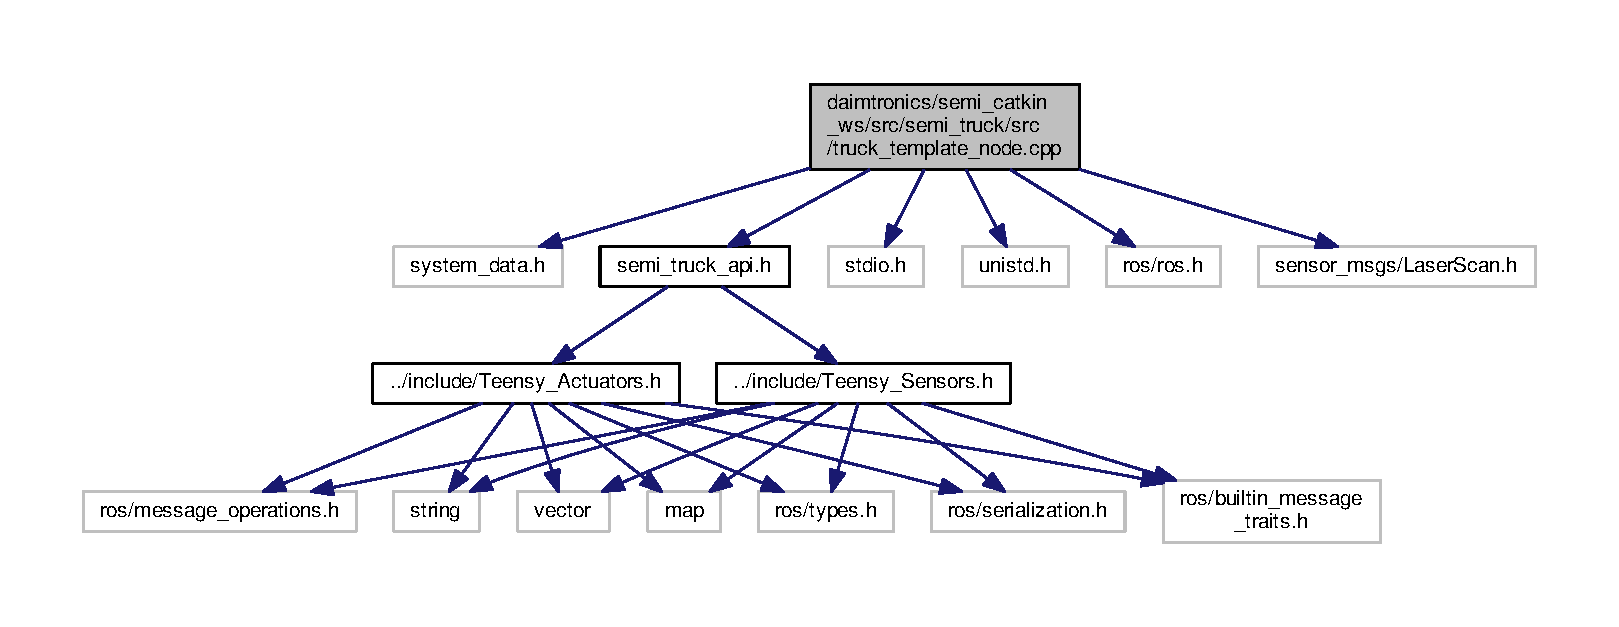
\includegraphics[width=350pt]{truck__template__node_8cpp__incl}
\end{center}
\end{figure}
\subsection*{Functions}
\begin{DoxyCompactItemize}
\item 
void \hyperlink{truck__template__node_8cpp_a8363f404c01d2a0626c10227fead51b5}{rplidar\+\_\+cb} (const sensor\+\_\+msgs\+::\+Laser\+Scan \&msg)
\item 
void \hyperlink{truck__template__node_8cpp_a8bc7378aaa9388d86ae7011d19657a02}{lidar\+\_\+lite\+\_\+cb} (const sensor\+\_\+msgs\+::\+Laser\+Scan \&msg)
\item 
void \hyperlink{truck__template__node_8cpp_acdc6ceefbb71e717b2ec560026e81433}{teensy\+\_\+sensors\+\_\+cb} (const \hyperlink{namespacesemi__truck_a8ffe15bf9a1e739c2242ac6d6feaa67f}{semi\+\_\+truck\+::\+Teensy\+\_\+\+Sensors} \&msg)
\item 
int \hyperlink{truck__template__node_8cpp_a3c04138a5bfe5d72780bb7e82a18e627}{main} (int argc, char $\ast$$\ast$argv)
\end{DoxyCompactItemize}


\subsection{Function Documentation}
\index{truck\+\_\+template\+\_\+node.\+cpp@{truck\+\_\+template\+\_\+node.\+cpp}!lidar\+\_\+lite\+\_\+cb@{lidar\+\_\+lite\+\_\+cb}}
\index{lidar\+\_\+lite\+\_\+cb@{lidar\+\_\+lite\+\_\+cb}!truck\+\_\+template\+\_\+node.\+cpp@{truck\+\_\+template\+\_\+node.\+cpp}}
\subsubsection[{\texorpdfstring{lidar\+\_\+lite\+\_\+cb(const sensor\+\_\+msgs\+::\+Laser\+Scan \&msg)}{lidar_lite_cb(const sensor_msgs::LaserScan &msg)}}]{\setlength{\rightskip}{0pt plus 5cm}void lidar\+\_\+lite\+\_\+cb (
\begin{DoxyParamCaption}
\item[{const sensor\+\_\+msgs\+::\+Laser\+Scan \&}]{msg}
\end{DoxyParamCaption}
)}\hypertarget{truck__template__node_8cpp_a8bc7378aaa9388d86ae7011d19657a02}{}\label{truck__template__node_8cpp_a8bc7378aaa9388d86ae7011d19657a02}
\index{truck\+\_\+template\+\_\+node.\+cpp@{truck\+\_\+template\+\_\+node.\+cpp}!main@{main}}
\index{main@{main}!truck\+\_\+template\+\_\+node.\+cpp@{truck\+\_\+template\+\_\+node.\+cpp}}
\subsubsection[{\texorpdfstring{main(int argc, char $\ast$$\ast$argv)}{main(int argc, char **argv)}}]{\setlength{\rightskip}{0pt plus 5cm}int main (
\begin{DoxyParamCaption}
\item[{int}]{argc, }
\item[{char $\ast$$\ast$}]{argv}
\end{DoxyParamCaption}
)}\hypertarget{truck__template__node_8cpp_a3c04138a5bfe5d72780bb7e82a18e627}{}\label{truck__template__node_8cpp_a3c04138a5bfe5d72780bb7e82a18e627}
\index{truck\+\_\+template\+\_\+node.\+cpp@{truck\+\_\+template\+\_\+node.\+cpp}!rplidar\+\_\+cb@{rplidar\+\_\+cb}}
\index{rplidar\+\_\+cb@{rplidar\+\_\+cb}!truck\+\_\+template\+\_\+node.\+cpp@{truck\+\_\+template\+\_\+node.\+cpp}}
\subsubsection[{\texorpdfstring{rplidar\+\_\+cb(const sensor\+\_\+msgs\+::\+Laser\+Scan \&msg)}{rplidar_cb(const sensor_msgs::LaserScan &msg)}}]{\setlength{\rightskip}{0pt plus 5cm}void rplidar\+\_\+cb (
\begin{DoxyParamCaption}
\item[{const sensor\+\_\+msgs\+::\+Laser\+Scan \&}]{msg}
\end{DoxyParamCaption}
)}\hypertarget{truck__template__node_8cpp_a8363f404c01d2a0626c10227fead51b5}{}\label{truck__template__node_8cpp_a8363f404c01d2a0626c10227fead51b5}
\index{truck\+\_\+template\+\_\+node.\+cpp@{truck\+\_\+template\+\_\+node.\+cpp}!teensy\+\_\+sensors\+\_\+cb@{teensy\+\_\+sensors\+\_\+cb}}
\index{teensy\+\_\+sensors\+\_\+cb@{teensy\+\_\+sensors\+\_\+cb}!truck\+\_\+template\+\_\+node.\+cpp@{truck\+\_\+template\+\_\+node.\+cpp}}
\subsubsection[{\texorpdfstring{teensy\+\_\+sensors\+\_\+cb(const semi\+\_\+truck\+::\+Teensy\+\_\+\+Sensors \&msg)}{teensy_sensors_cb(const semi_truck::Teensy_Sensors &msg)}}]{\setlength{\rightskip}{0pt plus 5cm}void teensy\+\_\+sensors\+\_\+cb (
\begin{DoxyParamCaption}
\item[{const {\bf semi\+\_\+truck\+::\+Teensy\+\_\+\+Sensors} \&}]{msg}
\end{DoxyParamCaption}
)}\hypertarget{truck__template__node_8cpp_acdc6ceefbb71e717b2ec560026e81433}{}\label{truck__template__node_8cpp_acdc6ceefbb71e717b2ec560026e81433}

\hypertarget{_8_d_s___store}{}\section{daimtronics/teensy\+\_\+chibios/src/.D\+S\+\_\+\+Store File Reference}
\label{_8_d_s___store}\index{daimtronics/teensy\+\_\+chibios/src/.\+D\+S\+\_\+\+Store@{daimtronics/teensy\+\_\+chibios/src/.\+D\+S\+\_\+\+Store}}

\hypertarget{fifth__wheel_8cpp}{}\section{daimtronics/teensy\+\_\+chibios/src/main/fifth\+\_\+wheel.cpp File Reference}
\label{fifth__wheel_8cpp}\index{daimtronics/teensy\+\_\+chibios/src/main/fifth\+\_\+wheel.\+cpp@{daimtronics/teensy\+\_\+chibios/src/main/fifth\+\_\+wheel.\+cpp}}
{\ttfamily \#include \char`\"{}include/fifth\+\_\+wheel.\+h\char`\"{}}\\*
{\ttfamily \#include \char`\"{}include/system\+\_\+data.\+h\char`\"{}}\\*
{\ttfamily \#include $<$Arduino.\+h$>$}\\*
{\ttfamily \#include $<$Servo.\+h$>$}\\*
Include dependency graph for fifth\+\_\+wheel.\+cpp\+:
\nopagebreak
\begin{figure}[H]
\begin{center}
\leavevmode
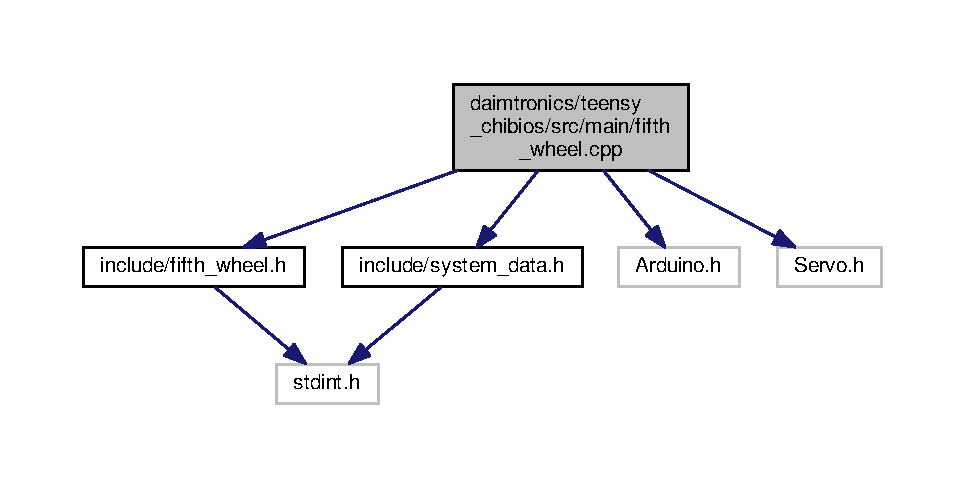
\includegraphics[width=350pt]{fifth__wheel_8cpp__incl}
\end{center}
\end{figure}
\subsection*{Macros}
\begin{DoxyCompactItemize}
\item 
\#define \hyperlink{fifth__wheel_8cpp_a45f4d39b01b3ce0c88fe3bd0f33bf059}{L\+O\+C\+K\+E\+D\+\_\+\+A\+N\+G\+LE}~0
\item 
\#define \hyperlink{fifth__wheel_8cpp_a412fd945ee985ffd091e6ba0d21200cf}{U\+N\+L\+O\+C\+K\+E\+D\+\_\+\+A\+N\+G\+LE}~180
\end{DoxyCompactItemize}
\subsection*{Functions}
\begin{DoxyCompactItemize}
\item 
void \hyperlink{fifth__wheel_8cpp_a14e7d99820fbf318dab31a2240485c4a}{fifth\+\_\+wheel\+\_\+loop\+\_\+fn} (int16\+\_\+t fifth\+\_\+output)
\item 
void \hyperlink{fifth__wheel_8cpp_a36146210c84097f03d4f940d28560ddb}{fifth\+\_\+wheel\+\_\+setup} (short fifth\+\_\+wheel\+\_\+pin)
\begin{DoxyCompactList}\small\item\em Set up the fifth wheel task to write to the pin attached to the fifth wheel, and to be in the locked position. \end{DoxyCompactList}\end{DoxyCompactItemize}


\subsection{Macro Definition Documentation}
\index{fifth\+\_\+wheel.\+cpp@{fifth\+\_\+wheel.\+cpp}!L\+O\+C\+K\+E\+D\+\_\+\+A\+N\+G\+LE@{L\+O\+C\+K\+E\+D\+\_\+\+A\+N\+G\+LE}}
\index{L\+O\+C\+K\+E\+D\+\_\+\+A\+N\+G\+LE@{L\+O\+C\+K\+E\+D\+\_\+\+A\+N\+G\+LE}!fifth\+\_\+wheel.\+cpp@{fifth\+\_\+wheel.\+cpp}}
\subsubsection[{\texorpdfstring{L\+O\+C\+K\+E\+D\+\_\+\+A\+N\+G\+LE}{LOCKED_ANGLE}}]{\setlength{\rightskip}{0pt plus 5cm}\#define L\+O\+C\+K\+E\+D\+\_\+\+A\+N\+G\+LE~0}\hypertarget{fifth__wheel_8cpp_a45f4d39b01b3ce0c88fe3bd0f33bf059}{}\label{fifth__wheel_8cpp_a45f4d39b01b3ce0c88fe3bd0f33bf059}
\index{fifth\+\_\+wheel.\+cpp@{fifth\+\_\+wheel.\+cpp}!U\+N\+L\+O\+C\+K\+E\+D\+\_\+\+A\+N\+G\+LE@{U\+N\+L\+O\+C\+K\+E\+D\+\_\+\+A\+N\+G\+LE}}
\index{U\+N\+L\+O\+C\+K\+E\+D\+\_\+\+A\+N\+G\+LE@{U\+N\+L\+O\+C\+K\+E\+D\+\_\+\+A\+N\+G\+LE}!fifth\+\_\+wheel.\+cpp@{fifth\+\_\+wheel.\+cpp}}
\subsubsection[{\texorpdfstring{U\+N\+L\+O\+C\+K\+E\+D\+\_\+\+A\+N\+G\+LE}{UNLOCKED_ANGLE}}]{\setlength{\rightskip}{0pt plus 5cm}\#define U\+N\+L\+O\+C\+K\+E\+D\+\_\+\+A\+N\+G\+LE~180}\hypertarget{fifth__wheel_8cpp_a412fd945ee985ffd091e6ba0d21200cf}{}\label{fifth__wheel_8cpp_a412fd945ee985ffd091e6ba0d21200cf}


\subsection{Function Documentation}
\index{fifth\+\_\+wheel.\+cpp@{fifth\+\_\+wheel.\+cpp}!fifth\+\_\+wheel\+\_\+loop\+\_\+fn@{fifth\+\_\+wheel\+\_\+loop\+\_\+fn}}
\index{fifth\+\_\+wheel\+\_\+loop\+\_\+fn@{fifth\+\_\+wheel\+\_\+loop\+\_\+fn}!fifth\+\_\+wheel.\+cpp@{fifth\+\_\+wheel.\+cpp}}
\subsubsection[{\texorpdfstring{fifth\+\_\+wheel\+\_\+loop\+\_\+fn(int16\+\_\+t fifth\+\_\+output)}{fifth_wheel_loop_fn(int16_t fifth_output)}}]{\setlength{\rightskip}{0pt plus 5cm}void fifth\+\_\+wheel\+\_\+loop\+\_\+fn (
\begin{DoxyParamCaption}
\item[{int16\+\_\+t}]{fifth\+\_\+output}
\end{DoxyParamCaption}
)}\hypertarget{fifth__wheel_8cpp_a14e7d99820fbf318dab31a2240485c4a}{}\label{fifth__wheel_8cpp_a14e7d99820fbf318dab31a2240485c4a}
The is the primary function controlling the fifth wheel. It reads the fifth\+\_\+output value form the system data and writes to the Servo for actuating between the two different angles.


\begin{DoxyParams}{Parameters}
{\em fifth\+\_\+output} & the output to the fifth wheel, which will be one of two values, either locked or unlocked \\
\hline
\end{DoxyParams}
\index{fifth\+\_\+wheel.\+cpp@{fifth\+\_\+wheel.\+cpp}!fifth\+\_\+wheel\+\_\+setup@{fifth\+\_\+wheel\+\_\+setup}}
\index{fifth\+\_\+wheel\+\_\+setup@{fifth\+\_\+wheel\+\_\+setup}!fifth\+\_\+wheel.\+cpp@{fifth\+\_\+wheel.\+cpp}}
\subsubsection[{\texorpdfstring{fifth\+\_\+wheel\+\_\+setup(short fifth\+\_\+wheel\+\_\+pin)}{fifth_wheel_setup(short fifth_wheel_pin)}}]{\setlength{\rightskip}{0pt plus 5cm}void fifth\+\_\+wheel\+\_\+setup (
\begin{DoxyParamCaption}
\item[{short}]{fifth\+\_\+wheel\+\_\+pin}
\end{DoxyParamCaption}
)}\hypertarget{fifth__wheel_8cpp_a36146210c84097f03d4f940d28560ddb}{}\label{fifth__wheel_8cpp_a36146210c84097f03d4f940d28560ddb}


Set up the fifth wheel task to write to the pin attached to the fifth wheel, and to be in the locked position. 


\begin{DoxyParams}{Parameters}
{\em fifth\+\_\+wheel\+\_\+pin} & The pin that signals a P\+WM to the fifth wheel servo. \\
\hline
\end{DoxyParams}

\hypertarget{hall__sensor_8cpp}{}\section{daimtronics/teensy\+\_\+chibios/src/main/hall\+\_\+sensor.cpp File Reference}
\label{hall__sensor_8cpp}\index{daimtronics/teensy\+\_\+chibios/src/main/hall\+\_\+sensor.\+cpp@{daimtronics/teensy\+\_\+chibios/src/main/hall\+\_\+sensor.\+cpp}}
{\ttfamily \#include \char`\"{}include/hall\+\_\+sensor.\+h\char`\"{}}\\*
{\ttfamily \#include $<$Arduino.\+h$>$}\\*
{\ttfamily \#include $<$Ch\+Rt.\+h$>$}\\*
Include dependency graph for hall\+\_\+sensor.\+cpp\+:
\nopagebreak
\begin{figure}[H]
\begin{center}
\leavevmode
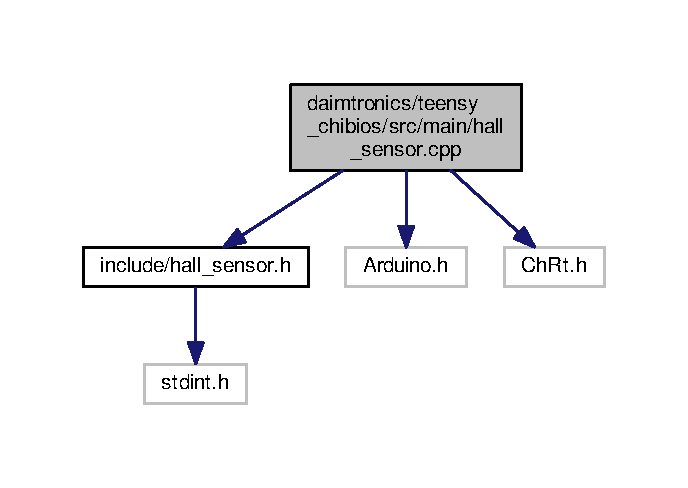
\includegraphics[width=330pt]{hall__sensor_8cpp__incl}
\end{center}
\end{figure}
\subsection*{Functions}
\begin{DoxyCompactItemize}
\item 
int16\+\_\+t \hyperlink{hall__sensor_8cpp_ac5350eff4f7be4591be4804922422dea}{hall\+\_\+sensor\+\_\+loop\+\_\+fn} (short Phase\+B\+\_\+pin, short Phase\+C\+\_\+pin)
\begin{DoxyCompactList}\small\item\em This is the primary function controlling the wheel speed sensor. It reads a Hall sensor that is built into the Tekin R8 Motor. This is a three phased motor (PhaseA, PhaseB, PhaseC). Each phase is offset 120 degrees from each other. Ticks will be incremented if the motor rotates forwards one full revolution, and decremented if it rotates backwards one revolution. \end{DoxyCompactList}\item 
void \hyperlink{hall__sensor_8cpp_a333d70b162bb762c6233815470f40d97}{hall\+\_\+sensor\+\_\+setup} (short Phase\+A\+\_\+pin, short Phase\+B\+\_\+pin, short Phase\+C\+\_\+pin)
\begin{DoxyCompactList}\small\item\em Set up the wheel speed task to read high or low values from the three pins attached to the Hall sensor (one for each phase). \end{DoxyCompactList}\end{DoxyCompactItemize}
\subsection*{Variables}
\begin{DoxyCompactItemize}
\item 
int16\+\_\+t \hyperlink{hall__sensor_8cpp_a4f9943e6ab43adfb6975aeb73911151b}{ticks} = 0
\end{DoxyCompactItemize}


\subsection{Function Documentation}
\index{hall\+\_\+sensor.\+cpp@{hall\+\_\+sensor.\+cpp}!hall\+\_\+sensor\+\_\+loop\+\_\+fn@{hall\+\_\+sensor\+\_\+loop\+\_\+fn}}
\index{hall\+\_\+sensor\+\_\+loop\+\_\+fn@{hall\+\_\+sensor\+\_\+loop\+\_\+fn}!hall\+\_\+sensor.\+cpp@{hall\+\_\+sensor.\+cpp}}
\subsubsection[{\texorpdfstring{hall\+\_\+sensor\+\_\+loop\+\_\+fn(short Phase\+B\+\_\+pin, short Phase\+C\+\_\+pin)}{hall_sensor_loop_fn(short PhaseB_pin, short PhaseC_pin)}}]{\setlength{\rightskip}{0pt plus 5cm}int16\+\_\+t hall\+\_\+sensor\+\_\+loop\+\_\+fn (
\begin{DoxyParamCaption}
\item[{short}]{Phase\+B\+\_\+pin, }
\item[{short}]{Phase\+C\+\_\+pin}
\end{DoxyParamCaption}
)}\hypertarget{hall__sensor_8cpp_ac5350eff4f7be4591be4804922422dea}{}\label{hall__sensor_8cpp_ac5350eff4f7be4591be4804922422dea}


This is the primary function controlling the wheel speed sensor. It reads a Hall sensor that is built into the Tekin R8 Motor. This is a three phased motor (PhaseA, PhaseB, PhaseC). Each phase is offset 120 degrees from each other. Ticks will be incremented if the motor rotates forwards one full revolution, and decremented if it rotates backwards one revolution. 

\begin{DoxyReturn}{Returns}
the current number of ticks that the sensor reads. 
\end{DoxyReturn}
\index{hall\+\_\+sensor.\+cpp@{hall\+\_\+sensor.\+cpp}!hall\+\_\+sensor\+\_\+setup@{hall\+\_\+sensor\+\_\+setup}}
\index{hall\+\_\+sensor\+\_\+setup@{hall\+\_\+sensor\+\_\+setup}!hall\+\_\+sensor.\+cpp@{hall\+\_\+sensor.\+cpp}}
\subsubsection[{\texorpdfstring{hall\+\_\+sensor\+\_\+setup(short Phase\+A\+\_\+pin, short Phase\+B\+\_\+pin, short Phase\+C\+\_\+pin)}{hall_sensor_setup(short PhaseA_pin, short PhaseB_pin, short PhaseC_pin)}}]{\setlength{\rightskip}{0pt plus 5cm}void hall\+\_\+sensor\+\_\+setup (
\begin{DoxyParamCaption}
\item[{short}]{Phase\+A\+\_\+pin, }
\item[{short}]{Phase\+B\+\_\+pin, }
\item[{short}]{Phase\+C\+\_\+pin}
\end{DoxyParamCaption}
)}\hypertarget{hall__sensor_8cpp_a333d70b162bb762c6233815470f40d97}{}\label{hall__sensor_8cpp_a333d70b162bb762c6233815470f40d97}


Set up the wheel speed task to read high or low values from the three pins attached to the Hall sensor (one for each phase). 


\begin{DoxyParams}{Parameters}
{\em Phase\+A\+\_\+pin} & An interrupt is triggered every time the Teensy read a leading edge for this phase. \\
\hline
{\em Phase\+B\+\_\+pin} & If this pin is high when the interrupt is triggered, the truck is going in reverse. \\
\hline
{\em Phase\+C\+\_\+pin} & If this pin is high when the interrupt is triggered, the truck is going forwards. \\
\hline
\end{DoxyParams}


\subsection{Variable Documentation}
\index{hall\+\_\+sensor.\+cpp@{hall\+\_\+sensor.\+cpp}!ticks@{ticks}}
\index{ticks@{ticks}!hall\+\_\+sensor.\+cpp@{hall\+\_\+sensor.\+cpp}}
\subsubsection[{\texorpdfstring{ticks}{ticks}}]{\setlength{\rightskip}{0pt plus 5cm}int16\+\_\+t ticks = 0}\hypertarget{hall__sensor_8cpp_a4f9943e6ab43adfb6975aeb73911151b}{}\label{hall__sensor_8cpp_a4f9943e6ab43adfb6975aeb73911151b}

\hypertarget{imu_8cpp}{}\section{daimtronics/teensy\+\_\+chibios/src/main/imu.cpp File Reference}
\label{imu_8cpp}\index{daimtronics/teensy\+\_\+chibios/src/main/imu.\+cpp@{daimtronics/teensy\+\_\+chibios/src/main/imu.\+cpp}}
{\ttfamily \#include \char`\"{}include/imu.\+h\char`\"{}}\\*
Include dependency graph for imu.\+cpp\+:
\nopagebreak
\begin{figure}[H]
\begin{center}
\leavevmode
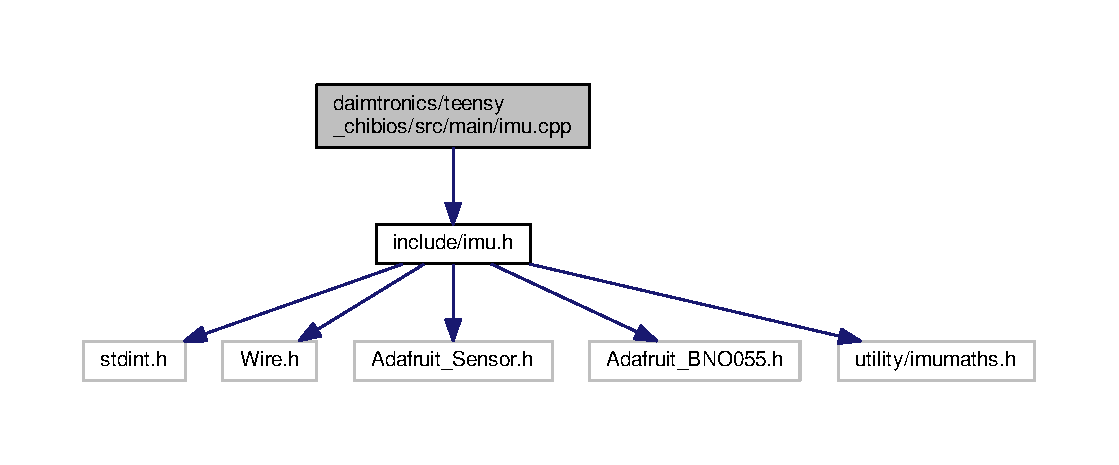
\includegraphics[width=350pt]{imu_8cpp__incl}
\end{center}
\end{figure}
\subsection*{Functions}
\begin{DoxyCompactItemize}
\item 
int16\+\_\+t \hyperlink{imu_8cpp_adc798e70ad6db427bf0636201422ad30}{imu\+\_\+loop\+\_\+fn} ()
\begin{DoxyCompactList}\small\item\em The primary function for the I\+MU that reads and returns heading data of the B\+N\+O055.\+The Adafruit\+\_\+\+B\+N\+O055 library does most of the work here. This function simply sets up a sets up an \char`\"{}event\char`\"{} variable to hold the I\+MU data. \end{DoxyCompactList}\item 
void \hyperlink{imu_8cpp_a1cf1c284c0587a36f6bed92f744a46a0}{imu\+\_\+setup} ()
\begin{DoxyCompactList}\small\item\em Initializes the B\+N\+O055 sensor. \end{DoxyCompactList}\item 
void \hyperlink{imu_8cpp_af2f32ad6a4e0d52e94d91a744a9c30aa}{print\+\_\+imu\+\_\+data} (sensors\+\_\+event\+\_\+t $\ast$event)
\begin{DoxyCompactList}\small\item\em A debugging function used to print out I\+MU orientation to the U\+SB serial device (usually the Arduino Serial Monitor). \end{DoxyCompactList}\end{DoxyCompactItemize}
\subsection*{Variables}
\begin{DoxyCompactItemize}
\item 
Adafruit\+\_\+\+B\+N\+O055 \hyperlink{imu_8cpp_a3365697089795e31b8ff89e70ff042ca}{bno} = Adafruit\+\_\+\+B\+N\+O055(55)
\begin{DoxyCompactList}\small\item\em A global variable, for the only Adafruit\+\_\+\+B\+N\+O055 object in the system. \end{DoxyCompactList}\end{DoxyCompactItemize}


\subsection{Function Documentation}
\index{imu.\+cpp@{imu.\+cpp}!imu\+\_\+loop\+\_\+fn@{imu\+\_\+loop\+\_\+fn}}
\index{imu\+\_\+loop\+\_\+fn@{imu\+\_\+loop\+\_\+fn}!imu.\+cpp@{imu.\+cpp}}
\subsubsection[{\texorpdfstring{imu\+\_\+loop\+\_\+fn()}{imu_loop_fn()}}]{\setlength{\rightskip}{0pt plus 5cm}int16\+\_\+t imu\+\_\+loop\+\_\+fn (
\begin{DoxyParamCaption}
{}
\end{DoxyParamCaption}
)}\hypertarget{imu_8cpp_adc798e70ad6db427bf0636201422ad30}{}\label{imu_8cpp_adc798e70ad6db427bf0636201422ad30}


The primary function for the I\+MU that reads and returns heading data of the B\+N\+O055.\+The Adafruit\+\_\+\+B\+N\+O055 library does most of the work here. This function simply sets up a sets up an \char`\"{}event\char`\"{} variable to hold the I\+MU data. 

\begin{DoxyReturn}{Returns}
an integer representing the heading angle in degrees 
\end{DoxyReturn}
\index{imu.\+cpp@{imu.\+cpp}!imu\+\_\+setup@{imu\+\_\+setup}}
\index{imu\+\_\+setup@{imu\+\_\+setup}!imu.\+cpp@{imu.\+cpp}}
\subsubsection[{\texorpdfstring{imu\+\_\+setup()}{imu_setup()}}]{\setlength{\rightskip}{0pt plus 5cm}void imu\+\_\+setup (
\begin{DoxyParamCaption}
{}
\end{DoxyParamCaption}
)}\hypertarget{imu_8cpp_a1cf1c284c0587a36f6bed92f744a46a0}{}\label{imu_8cpp_a1cf1c284c0587a36f6bed92f744a46a0}


Initializes the B\+N\+O055 sensor. 

\index{imu.\+cpp@{imu.\+cpp}!print\+\_\+imu\+\_\+data@{print\+\_\+imu\+\_\+data}}
\index{print\+\_\+imu\+\_\+data@{print\+\_\+imu\+\_\+data}!imu.\+cpp@{imu.\+cpp}}
\subsubsection[{\texorpdfstring{print\+\_\+imu\+\_\+data(sensors\+\_\+event\+\_\+t $\ast$event)}{print_imu_data(sensors_event_t *event)}}]{\setlength{\rightskip}{0pt plus 5cm}void print\+\_\+imu\+\_\+data (
\begin{DoxyParamCaption}
\item[{sensors\+\_\+event\+\_\+t $\ast$}]{event}
\end{DoxyParamCaption}
)}\hypertarget{imu_8cpp_af2f32ad6a4e0d52e94d91a744a9c30aa}{}\label{imu_8cpp_af2f32ad6a4e0d52e94d91a744a9c30aa}


A debugging function used to print out I\+MU orientation to the U\+SB serial device (usually the Arduino Serial Monitor). 



\subsection{Variable Documentation}
\index{imu.\+cpp@{imu.\+cpp}!bno@{bno}}
\index{bno@{bno}!imu.\+cpp@{imu.\+cpp}}
\subsubsection[{\texorpdfstring{bno}{bno}}]{\setlength{\rightskip}{0pt plus 5cm}Adafruit\+\_\+\+B\+N\+O055 bno = Adafruit\+\_\+\+B\+N\+O055(55)}\hypertarget{imu_8cpp_a3365697089795e31b8ff89e70ff042ca}{}\label{imu_8cpp_a3365697089795e31b8ff89e70ff042ca}


A global variable, for the only Adafruit\+\_\+\+B\+N\+O055 object in the system. 


\hypertarget{fifth__wheel_8h}{}\section{daimtronics/teensy\+\_\+chibios/src/main/include/fifth\+\_\+wheel.h File Reference}
\label{fifth__wheel_8h}\index{daimtronics/teensy\+\_\+chibios/src/main/include/fifth\+\_\+wheel.\+h@{daimtronics/teensy\+\_\+chibios/src/main/include/fifth\+\_\+wheel.\+h}}
{\ttfamily \#include $<$stdint.\+h$>$}\\*
Include dependency graph for fifth\+\_\+wheel.\+h\+:
\nopagebreak
\begin{figure}[H]
\begin{center}
\leavevmode
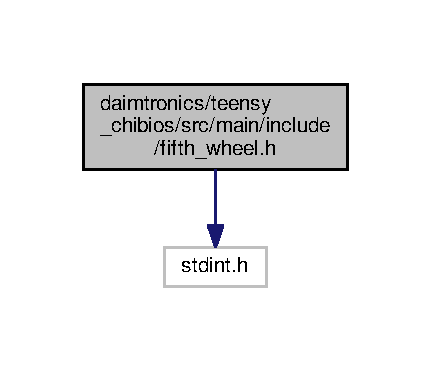
\includegraphics[width=207pt]{fifth__wheel_8h__incl}
\end{center}
\end{figure}
This graph shows which files directly or indirectly include this file\+:
\nopagebreak
\begin{figure}[H]
\begin{center}
\leavevmode
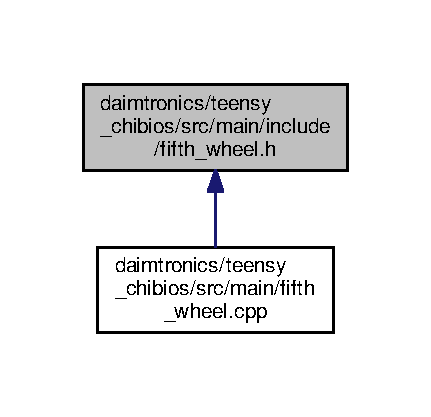
\includegraphics[width=207pt]{fifth__wheel_8h__dep__incl}
\end{center}
\end{figure}
\subsection*{Macros}
\begin{DoxyCompactItemize}
\item 
\#define \hyperlink{fifth__wheel_8h_a00de8f7e0b615f88335573ba3909583d}{L\+O\+C\+K\+ED}~1
\item 
\#define \hyperlink{fifth__wheel_8h_af0591d953a49374b660c9de8964825fe}{U\+N\+L\+O\+C\+K\+ED}~0
\end{DoxyCompactItemize}
\subsection*{Functions}
\begin{DoxyCompactItemize}
\item 
void \hyperlink{fifth__wheel_8h_a14e7d99820fbf318dab31a2240485c4a}{fifth\+\_\+wheel\+\_\+loop\+\_\+fn} (int16\+\_\+t fifth\+\_\+output)
\item 
void \hyperlink{fifth__wheel_8h_a36146210c84097f03d4f940d28560ddb}{fifth\+\_\+wheel\+\_\+setup} (short fifth\+\_\+wheel\+\_\+pin)
\begin{DoxyCompactList}\small\item\em Set up the fifth wheel task to write to the pin attached to the fifth wheel, and to be in the locked position. \end{DoxyCompactList}\end{DoxyCompactItemize}


\subsection{Macro Definition Documentation}
\index{fifth\+\_\+wheel.\+h@{fifth\+\_\+wheel.\+h}!L\+O\+C\+K\+ED@{L\+O\+C\+K\+ED}}
\index{L\+O\+C\+K\+ED@{L\+O\+C\+K\+ED}!fifth\+\_\+wheel.\+h@{fifth\+\_\+wheel.\+h}}
\subsubsection[{\texorpdfstring{L\+O\+C\+K\+ED}{LOCKED}}]{\setlength{\rightskip}{0pt plus 5cm}\#define L\+O\+C\+K\+ED~1}\hypertarget{fifth__wheel_8h_a00de8f7e0b615f88335573ba3909583d}{}\label{fifth__wheel_8h_a00de8f7e0b615f88335573ba3909583d}
\index{fifth\+\_\+wheel.\+h@{fifth\+\_\+wheel.\+h}!U\+N\+L\+O\+C\+K\+ED@{U\+N\+L\+O\+C\+K\+ED}}
\index{U\+N\+L\+O\+C\+K\+ED@{U\+N\+L\+O\+C\+K\+ED}!fifth\+\_\+wheel.\+h@{fifth\+\_\+wheel.\+h}}
\subsubsection[{\texorpdfstring{U\+N\+L\+O\+C\+K\+ED}{UNLOCKED}}]{\setlength{\rightskip}{0pt plus 5cm}\#define U\+N\+L\+O\+C\+K\+ED~0}\hypertarget{fifth__wheel_8h_af0591d953a49374b660c9de8964825fe}{}\label{fifth__wheel_8h_af0591d953a49374b660c9de8964825fe}


\subsection{Function Documentation}
\index{fifth\+\_\+wheel.\+h@{fifth\+\_\+wheel.\+h}!fifth\+\_\+wheel\+\_\+loop\+\_\+fn@{fifth\+\_\+wheel\+\_\+loop\+\_\+fn}}
\index{fifth\+\_\+wheel\+\_\+loop\+\_\+fn@{fifth\+\_\+wheel\+\_\+loop\+\_\+fn}!fifth\+\_\+wheel.\+h@{fifth\+\_\+wheel.\+h}}
\subsubsection[{\texorpdfstring{fifth\+\_\+wheel\+\_\+loop\+\_\+fn(int16\+\_\+t fifth\+\_\+output)}{fifth_wheel_loop_fn(int16_t fifth_output)}}]{\setlength{\rightskip}{0pt plus 5cm}void fifth\+\_\+wheel\+\_\+loop\+\_\+fn (
\begin{DoxyParamCaption}
\item[{int16\+\_\+t}]{fifth\+\_\+output}
\end{DoxyParamCaption}
)}\hypertarget{fifth__wheel_8h_a14e7d99820fbf318dab31a2240485c4a}{}\label{fifth__wheel_8h_a14e7d99820fbf318dab31a2240485c4a}
The is the primary function controlling the fifth wheel. It reads the fifth\+\_\+output value form the system data and writes to the Servo for actuating between the two different angles.


\begin{DoxyParams}{Parameters}
{\em fifth\+\_\+output} & the output to the fifth wheel, which will be one of two values, either locked or unlocked \\
\hline
\end{DoxyParams}
\index{fifth\+\_\+wheel.\+h@{fifth\+\_\+wheel.\+h}!fifth\+\_\+wheel\+\_\+setup@{fifth\+\_\+wheel\+\_\+setup}}
\index{fifth\+\_\+wheel\+\_\+setup@{fifth\+\_\+wheel\+\_\+setup}!fifth\+\_\+wheel.\+h@{fifth\+\_\+wheel.\+h}}
\subsubsection[{\texorpdfstring{fifth\+\_\+wheel\+\_\+setup(short fifth\+\_\+wheel\+\_\+pin)}{fifth_wheel_setup(short fifth_wheel_pin)}}]{\setlength{\rightskip}{0pt plus 5cm}void fifth\+\_\+wheel\+\_\+setup (
\begin{DoxyParamCaption}
\item[{short}]{fifth\+\_\+wheel\+\_\+pin}
\end{DoxyParamCaption}
)}\hypertarget{fifth__wheel_8h_a36146210c84097f03d4f940d28560ddb}{}\label{fifth__wheel_8h_a36146210c84097f03d4f940d28560ddb}


Set up the fifth wheel task to write to the pin attached to the fifth wheel, and to be in the locked position. 


\begin{DoxyParams}{Parameters}
{\em fifth\+\_\+wheel\+\_\+pin} & The pin that signals a P\+WM to the fifth wheel servo. \\
\hline
\end{DoxyParams}

\hypertarget{hall__sensor_8h}{}\section{daimtronics/teensy\+\_\+chibios/src/main/include/hall\+\_\+sensor.h File Reference}
\label{hall__sensor_8h}\index{daimtronics/teensy\+\_\+chibios/src/main/include/hall\+\_\+sensor.\+h@{daimtronics/teensy\+\_\+chibios/src/main/include/hall\+\_\+sensor.\+h}}
{\ttfamily \#include $<$stdint.\+h$>$}\\*
Include dependency graph for hall\+\_\+sensor.\+h\+:
\nopagebreak
\begin{figure}[H]
\begin{center}
\leavevmode
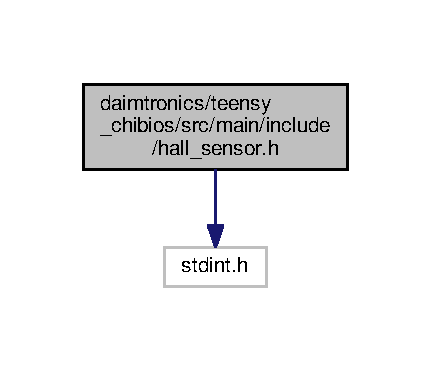
\includegraphics[width=207pt]{hall__sensor_8h__incl}
\end{center}
\end{figure}
This graph shows which files directly or indirectly include this file\+:
\nopagebreak
\begin{figure}[H]
\begin{center}
\leavevmode
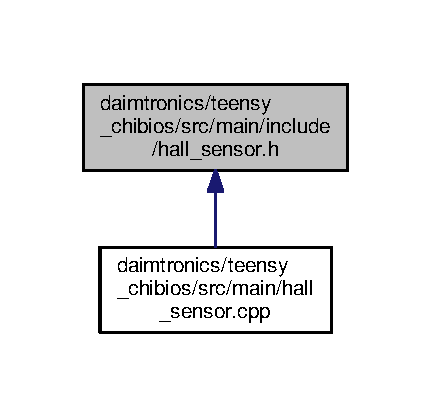
\includegraphics[width=207pt]{hall__sensor_8h__dep__incl}
\end{center}
\end{figure}
\subsection*{Functions}
\begin{DoxyCompactItemize}
\item 
int16\+\_\+t \hyperlink{hall__sensor_8h_ac5350eff4f7be4591be4804922422dea}{hall\+\_\+sensor\+\_\+loop\+\_\+fn} (short Phase\+B\+\_\+pin, short Phase\+C\+\_\+pin)
\begin{DoxyCompactList}\small\item\em This is the primary function controlling the wheel speed sensor. It reads a Hall sensor that is built into the Tekin R8 Motor. This is a three phased motor (PhaseA, PhaseB, PhaseC). Each phase is offset 120 degrees from each other. Ticks will be incremented if the motor rotates forwards one full revolution, and decremented if it rotates backwards one revolution. \end{DoxyCompactList}\item 
void \hyperlink{hall__sensor_8h_a333d70b162bb762c6233815470f40d97}{hall\+\_\+sensor\+\_\+setup} (short Phase\+A\+\_\+pin, short Phase\+B\+\_\+pin, short Phase\+C\+\_\+pin)
\begin{DoxyCompactList}\small\item\em Set up the wheel speed task to read high or low values from the three pins attached to the Hall sensor (one for each phase). \end{DoxyCompactList}\end{DoxyCompactItemize}


\subsection{Function Documentation}
\index{hall\+\_\+sensor.\+h@{hall\+\_\+sensor.\+h}!hall\+\_\+sensor\+\_\+loop\+\_\+fn@{hall\+\_\+sensor\+\_\+loop\+\_\+fn}}
\index{hall\+\_\+sensor\+\_\+loop\+\_\+fn@{hall\+\_\+sensor\+\_\+loop\+\_\+fn}!hall\+\_\+sensor.\+h@{hall\+\_\+sensor.\+h}}
\subsubsection[{\texorpdfstring{hall\+\_\+sensor\+\_\+loop\+\_\+fn(short Phase\+B\+\_\+pin, short Phase\+C\+\_\+pin)}{hall_sensor_loop_fn(short PhaseB_pin, short PhaseC_pin)}}]{\setlength{\rightskip}{0pt plus 5cm}int16\+\_\+t hall\+\_\+sensor\+\_\+loop\+\_\+fn (
\begin{DoxyParamCaption}
\item[{short}]{Phase\+B\+\_\+pin, }
\item[{short}]{Phase\+C\+\_\+pin}
\end{DoxyParamCaption}
)}\hypertarget{hall__sensor_8h_ac5350eff4f7be4591be4804922422dea}{}\label{hall__sensor_8h_ac5350eff4f7be4591be4804922422dea}


This is the primary function controlling the wheel speed sensor. It reads a Hall sensor that is built into the Tekin R8 Motor. This is a three phased motor (PhaseA, PhaseB, PhaseC). Each phase is offset 120 degrees from each other. Ticks will be incremented if the motor rotates forwards one full revolution, and decremented if it rotates backwards one revolution. 

\begin{DoxyReturn}{Returns}
the current number of ticks that the sensor reads. 
\end{DoxyReturn}
\index{hall\+\_\+sensor.\+h@{hall\+\_\+sensor.\+h}!hall\+\_\+sensor\+\_\+setup@{hall\+\_\+sensor\+\_\+setup}}
\index{hall\+\_\+sensor\+\_\+setup@{hall\+\_\+sensor\+\_\+setup}!hall\+\_\+sensor.\+h@{hall\+\_\+sensor.\+h}}
\subsubsection[{\texorpdfstring{hall\+\_\+sensor\+\_\+setup(short Phase\+A\+\_\+pin, short Phase\+B\+\_\+pin, short Phase\+C\+\_\+pin)}{hall_sensor_setup(short PhaseA_pin, short PhaseB_pin, short PhaseC_pin)}}]{\setlength{\rightskip}{0pt plus 5cm}void hall\+\_\+sensor\+\_\+setup (
\begin{DoxyParamCaption}
\item[{short}]{Phase\+A\+\_\+pin, }
\item[{short}]{Phase\+B\+\_\+pin, }
\item[{short}]{Phase\+C\+\_\+pin}
\end{DoxyParamCaption}
)}\hypertarget{hall__sensor_8h_a333d70b162bb762c6233815470f40d97}{}\label{hall__sensor_8h_a333d70b162bb762c6233815470f40d97}


Set up the wheel speed task to read high or low values from the three pins attached to the Hall sensor (one for each phase). 


\begin{DoxyParams}{Parameters}
{\em Phase\+A\+\_\+pin} & An interrupt is triggered every time the Teensy read a leading edge for this phase. \\
\hline
{\em Phase\+B\+\_\+pin} & If this pin is high when the interrupt is triggered, the truck is going in reverse. \\
\hline
{\em Phase\+C\+\_\+pin} & If this pin is high when the interrupt is triggered, the truck is going forwards. \\
\hline
\end{DoxyParams}

\hypertarget{imu_8h}{}\section{daimtronics/teensy\+\_\+chibios/src/main/include/imu.h File Reference}
\label{imu_8h}\index{daimtronics/teensy\+\_\+chibios/src/main/include/imu.\+h@{daimtronics/teensy\+\_\+chibios/src/main/include/imu.\+h}}
{\ttfamily \#include $<$stdint.\+h$>$}\\*
{\ttfamily \#include $<$Wire.\+h$>$}\\*
{\ttfamily \#include $<$Adafruit\+\_\+\+Sensor.\+h$>$}\\*
{\ttfamily \#include $<$Adafruit\+\_\+\+B\+N\+O055.\+h$>$}\\*
{\ttfamily \#include $<$utility/imumaths.\+h$>$}\\*
Include dependency graph for imu.\+h\+:
\nopagebreak
\begin{figure}[H]
\begin{center}
\leavevmode
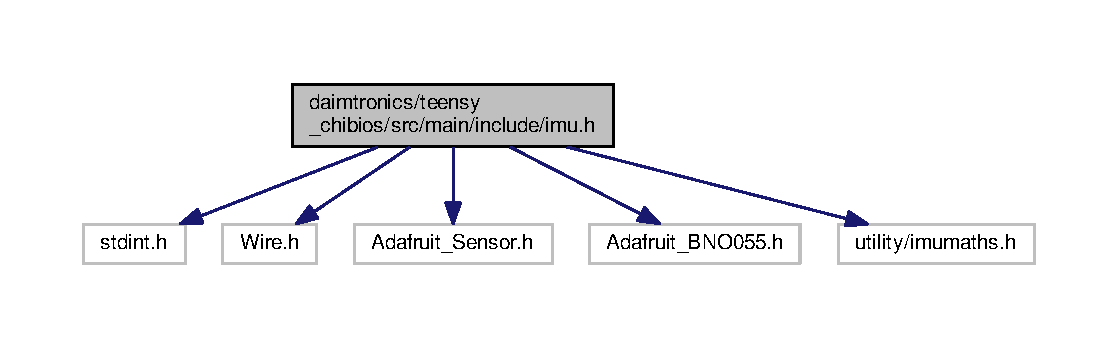
\includegraphics[width=350pt]{imu_8h__incl}
\end{center}
\end{figure}
This graph shows which files directly or indirectly include this file\+:
\nopagebreak
\begin{figure}[H]
\begin{center}
\leavevmode
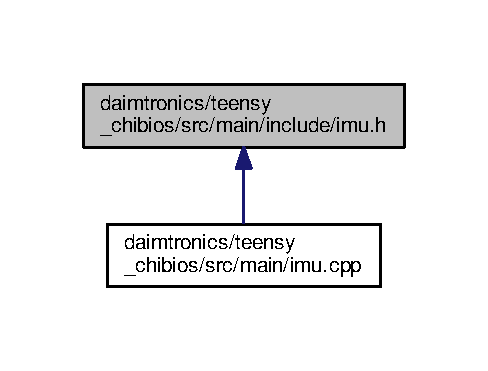
\includegraphics[width=234pt]{imu_8h__dep__incl}
\end{center}
\end{figure}
\subsection*{Functions}
\begin{DoxyCompactItemize}
\item 
short \hyperlink{imu_8h_ae18ba44402a9a2374a56d312f022d920}{imu\+\_\+loop\+\_\+fn} ()
\begin{DoxyCompactList}\small\item\em The primary function for the I\+MU that reads and returns heading data of the B\+N\+O055.\+The Adafruit\+\_\+\+B\+N\+O055 library does most of the work here. This function simply sets up a sets up an \char`\"{}event\char`\"{} variable to hold the I\+MU data. \end{DoxyCompactList}\item 
void \hyperlink{imu_8h_a1cf1c284c0587a36f6bed92f744a46a0}{imu\+\_\+setup} ()
\begin{DoxyCompactList}\small\item\em Initializes the B\+N\+O055 sensor. \end{DoxyCompactList}\item 
void \hyperlink{imu_8h_af2f32ad6a4e0d52e94d91a744a9c30aa}{print\+\_\+imu\+\_\+data} (sensors\+\_\+event\+\_\+t $\ast$event)
\begin{DoxyCompactList}\small\item\em A debugging function used to print out I\+MU orientation to the U\+SB serial device (usually the Arduino Serial Monitor). \end{DoxyCompactList}\end{DoxyCompactItemize}


\subsection{Function Documentation}
\index{imu.\+h@{imu.\+h}!imu\+\_\+loop\+\_\+fn@{imu\+\_\+loop\+\_\+fn}}
\index{imu\+\_\+loop\+\_\+fn@{imu\+\_\+loop\+\_\+fn}!imu.\+h@{imu.\+h}}
\subsubsection[{\texorpdfstring{imu\+\_\+loop\+\_\+fn()}{imu_loop_fn()}}]{\setlength{\rightskip}{0pt plus 5cm}short imu\+\_\+loop\+\_\+fn (
\begin{DoxyParamCaption}
{}
\end{DoxyParamCaption}
)}\hypertarget{imu_8h_ae18ba44402a9a2374a56d312f022d920}{}\label{imu_8h_ae18ba44402a9a2374a56d312f022d920}


The primary function for the I\+MU that reads and returns heading data of the B\+N\+O055.\+The Adafruit\+\_\+\+B\+N\+O055 library does most of the work here. This function simply sets up a sets up an \char`\"{}event\char`\"{} variable to hold the I\+MU data. 

\begin{DoxyReturn}{Returns}
an integer representing the heading angle in degrees 
\end{DoxyReturn}
\index{imu.\+h@{imu.\+h}!imu\+\_\+setup@{imu\+\_\+setup}}
\index{imu\+\_\+setup@{imu\+\_\+setup}!imu.\+h@{imu.\+h}}
\subsubsection[{\texorpdfstring{imu\+\_\+setup()}{imu_setup()}}]{\setlength{\rightskip}{0pt plus 5cm}void imu\+\_\+setup (
\begin{DoxyParamCaption}
{}
\end{DoxyParamCaption}
)}\hypertarget{imu_8h_a1cf1c284c0587a36f6bed92f744a46a0}{}\label{imu_8h_a1cf1c284c0587a36f6bed92f744a46a0}


Initializes the B\+N\+O055 sensor. 

\index{imu.\+h@{imu.\+h}!print\+\_\+imu\+\_\+data@{print\+\_\+imu\+\_\+data}}
\index{print\+\_\+imu\+\_\+data@{print\+\_\+imu\+\_\+data}!imu.\+h@{imu.\+h}}
\subsubsection[{\texorpdfstring{print\+\_\+imu\+\_\+data(sensors\+\_\+event\+\_\+t $\ast$event)}{print_imu_data(sensors_event_t *event)}}]{\setlength{\rightskip}{0pt plus 5cm}void print\+\_\+imu\+\_\+data (
\begin{DoxyParamCaption}
\item[{sensors\+\_\+event\+\_\+t $\ast$}]{event}
\end{DoxyParamCaption}
)}\hypertarget{imu_8h_af2f32ad6a4e0d52e94d91a744a9c30aa}{}\label{imu_8h_af2f32ad6a4e0d52e94d91a744a9c30aa}


A debugging function used to print out I\+MU orientation to the U\+SB serial device (usually the Arduino Serial Monitor). 


\hypertarget{motor__driver_8h}{}\section{daimtronics/teensy\+\_\+chibios/src/main/include/motor\+\_\+driver.h File Reference}
\label{motor__driver_8h}\index{daimtronics/teensy\+\_\+chibios/src/main/include/motor\+\_\+driver.\+h@{daimtronics/teensy\+\_\+chibios/src/main/include/motor\+\_\+driver.\+h}}
{\ttfamily \#include $<$stdint.\+h$>$}\\*
Include dependency graph for motor\+\_\+driver.\+h\+:
\nopagebreak
\begin{figure}[H]
\begin{center}
\leavevmode
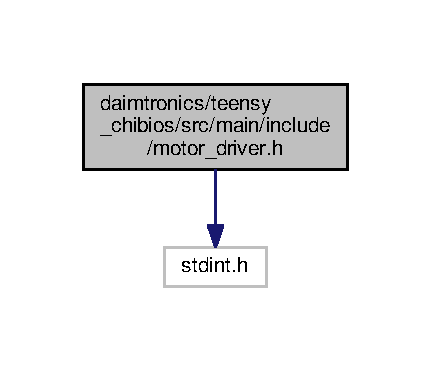
\includegraphics[width=207pt]{motor__driver_8h__incl}
\end{center}
\end{figure}
This graph shows which files directly or indirectly include this file\+:
\nopagebreak
\begin{figure}[H]
\begin{center}
\leavevmode
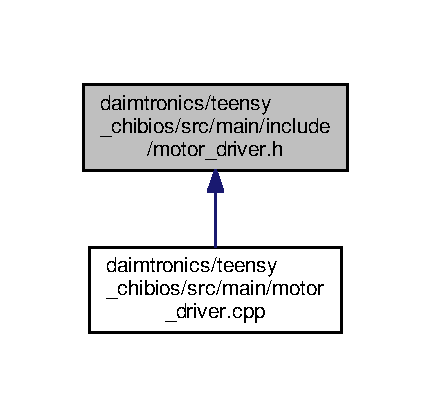
\includegraphics[width=207pt]{motor__driver_8h__dep__incl}
\end{center}
\end{figure}
\subsection*{Functions}
\begin{DoxyCompactItemize}
\item 
void \hyperlink{motor__driver_8h_a47f1b6dfc5a8fd9aac0efb348be5fb21}{motor\+\_\+driver\+\_\+loop\+\_\+fn} (int16\+\_\+t motor\+\_\+output)
\begin{DoxyCompactList}\small\item\em This is the primary function controlling the motor. It reads the motor output value from the system data and controls the motor with this value. \end{DoxyCompactList}\item 
int16\+\_\+t \hyperlink{motor__driver_8h_af8b67084d01c0aae1b2a7ef168956555}{scale\+\_\+output} (int16\+\_\+t motor\+\_\+output)
\begin{DoxyCompactList}\small\item\em Scales a value coming from the pi between -\/100 and 100 to between 0 and 180 for what the Servo library requires. \end{DoxyCompactList}\item 
void \hyperlink{motor__driver_8h_a736a79afc1c9cc88f7cc3de60f676b3e}{motor\+\_\+driver\+\_\+setup} (short motor\+\_\+pin)
\begin{DoxyCompactList}\small\item\em Set up the motor driver task to write to the pin attached to the motor, and to be in the locked position. It also outputs a value corresponding to zero torque. \end{DoxyCompactList}\item 
int16\+\_\+t \hyperlink{motor__driver_8h_ada070d71dced9dccaf66288fb47b1ac0}{stop\+\_\+motor} (int16\+\_\+t wheel\+\_\+speed, int16\+\_\+t time\+\_\+step)
\begin{DoxyCompactList}\small\item\em Runs a control loop to stop the motor based on the reported wheel speed, and returns a value to be output to the motor. \end{DoxyCompactList}\end{DoxyCompactItemize}


\subsection{Function Documentation}
\index{motor\+\_\+driver.\+h@{motor\+\_\+driver.\+h}!motor\+\_\+driver\+\_\+loop\+\_\+fn@{motor\+\_\+driver\+\_\+loop\+\_\+fn}}
\index{motor\+\_\+driver\+\_\+loop\+\_\+fn@{motor\+\_\+driver\+\_\+loop\+\_\+fn}!motor\+\_\+driver.\+h@{motor\+\_\+driver.\+h}}
\subsubsection[{\texorpdfstring{motor\+\_\+driver\+\_\+loop\+\_\+fn(int16\+\_\+t motor\+\_\+output)}{motor_driver_loop_fn(int16_t motor_output)}}]{\setlength{\rightskip}{0pt plus 5cm}void motor\+\_\+driver\+\_\+loop\+\_\+fn (
\begin{DoxyParamCaption}
\item[{int16\+\_\+t}]{motor\+\_\+output}
\end{DoxyParamCaption}
)}\hypertarget{motor__driver_8h_a47f1b6dfc5a8fd9aac0efb348be5fb21}{}\label{motor__driver_8h_a47f1b6dfc5a8fd9aac0efb348be5fb21}


This is the primary function controlling the motor. It reads the motor output value from the system data and controls the motor with this value. 


\begin{DoxyParams}{Parameters}
{\em motor\+\_\+output} & the output to the motor \\
\hline
\end{DoxyParams}
\index{motor\+\_\+driver.\+h@{motor\+\_\+driver.\+h}!motor\+\_\+driver\+\_\+setup@{motor\+\_\+driver\+\_\+setup}}
\index{motor\+\_\+driver\+\_\+setup@{motor\+\_\+driver\+\_\+setup}!motor\+\_\+driver.\+h@{motor\+\_\+driver.\+h}}
\subsubsection[{\texorpdfstring{motor\+\_\+driver\+\_\+setup(short motor\+\_\+pin)}{motor_driver_setup(short motor_pin)}}]{\setlength{\rightskip}{0pt plus 5cm}void motor\+\_\+driver\+\_\+setup (
\begin{DoxyParamCaption}
\item[{short}]{motor\+\_\+pin}
\end{DoxyParamCaption}
)}\hypertarget{motor__driver_8h_a736a79afc1c9cc88f7cc3de60f676b3e}{}\label{motor__driver_8h_a736a79afc1c9cc88f7cc3de60f676b3e}


Set up the motor driver task to write to the pin attached to the motor, and to be in the locked position. It also outputs a value corresponding to zero torque. 


\begin{DoxyParams}{Parameters}
{\em motor\+\_\+pin} & The pin sends a P\+WM signal to the motor. \\
\hline
\end{DoxyParams}
\index{motor\+\_\+driver.\+h@{motor\+\_\+driver.\+h}!scale\+\_\+output@{scale\+\_\+output}}
\index{scale\+\_\+output@{scale\+\_\+output}!motor\+\_\+driver.\+h@{motor\+\_\+driver.\+h}}
\subsubsection[{\texorpdfstring{scale\+\_\+output(int16\+\_\+t motor\+\_\+output)}{scale_output(int16_t motor_output)}}]{\setlength{\rightskip}{0pt plus 5cm}int16\+\_\+t scale\+\_\+output (
\begin{DoxyParamCaption}
\item[{int16\+\_\+t}]{motor\+\_\+output}
\end{DoxyParamCaption}
)}\hypertarget{motor__driver_8h_af8b67084d01c0aae1b2a7ef168956555}{}\label{motor__driver_8h_af8b67084d01c0aae1b2a7ef168956555}


Scales a value coming from the pi between -\/100 and 100 to between 0 and 180 for what the Servo library requires. 


\begin{DoxyParams}{Parameters}
{\em motor\+\_\+output} & An input value, ideally between -\/100 and 100 (although it will be limited to -\/100 or 100 if outside this range \\
\hline
\end{DoxyParams}
\begin{DoxyReturn}{Returns}
a value to output to the motor between 0 and 180 
\end{DoxyReturn}
\index{motor\+\_\+driver.\+h@{motor\+\_\+driver.\+h}!stop\+\_\+motor@{stop\+\_\+motor}}
\index{stop\+\_\+motor@{stop\+\_\+motor}!motor\+\_\+driver.\+h@{motor\+\_\+driver.\+h}}
\subsubsection[{\texorpdfstring{stop\+\_\+motor(int16\+\_\+t wheel\+\_\+speed, int16\+\_\+t time\+\_\+step)}{stop_motor(int16_t wheel_speed, int16_t time_step)}}]{\setlength{\rightskip}{0pt plus 5cm}int16\+\_\+t stop\+\_\+motor (
\begin{DoxyParamCaption}
\item[{int16\+\_\+t}]{wheel\+\_\+speed, }
\item[{int16\+\_\+t}]{time\+\_\+step}
\end{DoxyParamCaption}
)}\hypertarget{motor__driver_8h_ada070d71dced9dccaf66288fb47b1ac0}{}\label{motor__driver_8h_ada070d71dced9dccaf66288fb47b1ac0}


Runs a control loop to stop the motor based on the reported wheel speed, and returns a value to be output to the motor. 


\begin{DoxyParams}{Parameters}
{\em wheel\+\_\+speed} & speed of the truck read by the wheel speed sensor \\
\hline
{\em time\+\_\+step} & number of millis since the last time this task ran; used in integral control \\
\hline
\end{DoxyParams}
\begin{DoxyReturn}{Returns}
the output to the motor 
\end{DoxyReturn}

\hypertarget{range__finder_8h}{}\section{daimtronics/teensy\+\_\+chibios/src/main/include/range\+\_\+finder.h File Reference}
\label{range__finder_8h}\index{daimtronics/teensy\+\_\+chibios/src/main/include/range\+\_\+finder.\+h@{daimtronics/teensy\+\_\+chibios/src/main/include/range\+\_\+finder.\+h}}
{\ttfamily \#include $<$stdint.\+h$>$}\\*
Include dependency graph for range\+\_\+finder.\+h\+:
\nopagebreak
\begin{figure}[H]
\begin{center}
\leavevmode
\includegraphics[width=207pt]{range__finder_8h__incl}
\end{center}
\end{figure}
This graph shows which files directly or indirectly include this file\+:
\nopagebreak
\begin{figure}[H]
\begin{center}
\leavevmode
\includegraphics[width=207pt]{range__finder_8h__dep__incl}
\end{center}
\end{figure}
\subsection*{Functions}
\begin{DoxyCompactItemize}
\item 
long \hyperlink{range__finder_8h_a0d1a577ed4abf6a70b901350c16a2d23}{range\+\_\+finder\+\_\+loop\+\_\+fn} (short urf\+\_\+echo\+\_\+pin)
\item 
void \hyperlink{range__finder_8h_a521545ba36c9e983d134c77012323425}{range\+\_\+finder\+\_\+ping} (short urf\+\_\+trig\+\_\+pin)
\item 
void \hyperlink{range__finder_8h_afcf7c8f62f64d24ae76873d3a9471094}{range\+\_\+finder\+\_\+setup} (short urf\+\_\+trig\+\_\+pin)
\end{DoxyCompactItemize}


\subsection{Function Documentation}
\index{range\+\_\+finder.\+h@{range\+\_\+finder.\+h}!range\+\_\+finder\+\_\+loop\+\_\+fn@{range\+\_\+finder\+\_\+loop\+\_\+fn}}
\index{range\+\_\+finder\+\_\+loop\+\_\+fn@{range\+\_\+finder\+\_\+loop\+\_\+fn}!range\+\_\+finder.\+h@{range\+\_\+finder.\+h}}
\subsubsection[{\texorpdfstring{range\+\_\+finder\+\_\+loop\+\_\+fn(short urf\+\_\+echo\+\_\+pin)}{range_finder_loop_fn(short urf_echo_pin)}}]{\setlength{\rightskip}{0pt plus 5cm}long range\+\_\+finder\+\_\+loop\+\_\+fn (
\begin{DoxyParamCaption}
\item[{short}]{urf\+\_\+echo\+\_\+pin}
\end{DoxyParamCaption}
)}\hypertarget{range__finder_8h_a0d1a577ed4abf6a70b901350c16a2d23}{}\label{range__finder_8h_a0d1a577ed4abf6a70b901350c16a2d23}
This is the primary function controlling the U\+R\+Fs. It reads a value representing a distance to an object from the U\+RF sensor and returns that value

\begin{DoxyReturn}{Returns}
distance to object 
\end{DoxyReturn}
\index{range\+\_\+finder.\+h@{range\+\_\+finder.\+h}!range\+\_\+finder\+\_\+ping@{range\+\_\+finder\+\_\+ping}}
\index{range\+\_\+finder\+\_\+ping@{range\+\_\+finder\+\_\+ping}!range\+\_\+finder.\+h@{range\+\_\+finder.\+h}}
\subsubsection[{\texorpdfstring{range\+\_\+finder\+\_\+ping(short urf\+\_\+trig\+\_\+pin)}{range_finder_ping(short urf_trig_pin)}}]{\setlength{\rightskip}{0pt plus 5cm}void range\+\_\+finder\+\_\+ping (
\begin{DoxyParamCaption}
\item[{short}]{urf\+\_\+trig\+\_\+pin}
\end{DoxyParamCaption}
)}\hypertarget{range__finder_8h_a521545ba36c9e983d134c77012323425}{}\label{range__finder_8h_a521545ba36c9e983d134c77012323425}
\index{range\+\_\+finder.\+h@{range\+\_\+finder.\+h}!range\+\_\+finder\+\_\+setup@{range\+\_\+finder\+\_\+setup}}
\index{range\+\_\+finder\+\_\+setup@{range\+\_\+finder\+\_\+setup}!range\+\_\+finder.\+h@{range\+\_\+finder.\+h}}
\subsubsection[{\texorpdfstring{range\+\_\+finder\+\_\+setup(short urf\+\_\+trig\+\_\+pin)}{range_finder_setup(short urf_trig_pin)}}]{\setlength{\rightskip}{0pt plus 5cm}void range\+\_\+finder\+\_\+setup (
\begin{DoxyParamCaption}
\item[{short}]{urf\+\_\+trig\+\_\+pin}
\end{DoxyParamCaption}
)}\hypertarget{range__finder_8h_afcf7c8f62f64d24ae76873d3a9471094}{}\label{range__finder_8h_afcf7c8f62f64d24ae76873d3a9471094}

\hypertarget{_r_c__receiver_8h}{}\section{daimtronics/teensy\+\_\+chibios/src/main/include/\+R\+C\+\_\+receiver.h File Reference}
\label{_r_c__receiver_8h}\index{daimtronics/teensy\+\_\+chibios/src/main/include/\+R\+C\+\_\+receiver.\+h@{daimtronics/teensy\+\_\+chibios/src/main/include/\+R\+C\+\_\+receiver.\+h}}
{\ttfamily \#include $<$stdint.\+h$>$}\\*
Include dependency graph for R\+C\+\_\+receiver.\+h\+:
\nopagebreak
\begin{figure}[H]
\begin{center}
\leavevmode
\includegraphics[width=207pt]{_r_c__receiver_8h__incl}
\end{center}
\end{figure}
This graph shows which files directly or indirectly include this file\+:
\nopagebreak
\begin{figure}[H]
\begin{center}
\leavevmode
\includegraphics[width=207pt]{_r_c__receiver_8h__dep__incl}
\end{center}
\end{figure}
\subsection*{Functions}
\begin{DoxyCompactItemize}
\item 
int16\+\_\+t \hyperlink{_r_c__receiver_8h_a23c4334055a956a8aebf098e4b221b8e}{R\+C\+\_\+receiver\+\_\+\+S\+W1\+\_\+fn} (short P\+W\+M\+\_\+\+P\+IN)
\begin{DoxyCompactList}\small\item\em This is the primary function reading Switch 1 on the receiver. It reads a P\+WM signal that the RC receiver receives from the RC controller. Based on the specific timing of the P\+WM, a deadman mode (either deadman switch pressed or not pressed) is selected to send to the rest of the platform. \end{DoxyCompactList}\item 
int16\+\_\+t \hyperlink{_r_c__receiver_8h_a145bffdd8c1a4131d81c20e56cbb69dd}{R\+C\+\_\+receiver\+\_\+\+S\+W2\+\_\+fn} (short P\+W\+M\+\_\+\+P\+IN)
\item 
int16\+\_\+t \hyperlink{_r_c__receiver_8h_a268ff21fe35dba113741705a7b281ec0}{R\+C\+\_\+receiver\+\_\+\+S\+W3\+\_\+fn} (short P\+W\+M\+\_\+\+P\+IN)
\begin{DoxyCompactList}\small\item\em This is the primary function controlling the RC receiver. It reads a P\+WM signal that the RC receiver receives from the RC controller. Based on the specific timing of the P\+WM, a drive mode (either manual or one of the autonomous algorithms on the Pi) is selected to control the vehicle. \end{DoxyCompactList}\item 
void \hyperlink{_r_c__receiver_8h_a45897a7e81dfbed4ed1594172b3a0345}{R\+C\+\_\+receiver\+\_\+setup} ()
\end{DoxyCompactItemize}


\subsection{Function Documentation}
\index{R\+C\+\_\+receiver.\+h@{R\+C\+\_\+receiver.\+h}!R\+C\+\_\+receiver\+\_\+setup@{R\+C\+\_\+receiver\+\_\+setup}}
\index{R\+C\+\_\+receiver\+\_\+setup@{R\+C\+\_\+receiver\+\_\+setup}!R\+C\+\_\+receiver.\+h@{R\+C\+\_\+receiver.\+h}}
\subsubsection[{\texorpdfstring{R\+C\+\_\+receiver\+\_\+setup()}{RC_receiver_setup()}}]{\setlength{\rightskip}{0pt plus 5cm}void R\+C\+\_\+receiver\+\_\+setup (
\begin{DoxyParamCaption}
{}
\end{DoxyParamCaption}
)}\hypertarget{_r_c__receiver_8h_a45897a7e81dfbed4ed1594172b3a0345}{}\label{_r_c__receiver_8h_a45897a7e81dfbed4ed1594172b3a0345}
\index{R\+C\+\_\+receiver.\+h@{R\+C\+\_\+receiver.\+h}!R\+C\+\_\+receiver\+\_\+\+S\+W1\+\_\+fn@{R\+C\+\_\+receiver\+\_\+\+S\+W1\+\_\+fn}}
\index{R\+C\+\_\+receiver\+\_\+\+S\+W1\+\_\+fn@{R\+C\+\_\+receiver\+\_\+\+S\+W1\+\_\+fn}!R\+C\+\_\+receiver.\+h@{R\+C\+\_\+receiver.\+h}}
\subsubsection[{\texorpdfstring{R\+C\+\_\+receiver\+\_\+\+S\+W1\+\_\+fn(short P\+W\+M\+\_\+\+P\+I\+N)}{RC_receiver_SW1_fn(short PWM_PIN)}}]{\setlength{\rightskip}{0pt plus 5cm}int16\+\_\+t R\+C\+\_\+receiver\+\_\+\+S\+W1\+\_\+fn (
\begin{DoxyParamCaption}
\item[{short}]{P\+W\+M\+\_\+\+P\+IN}
\end{DoxyParamCaption}
)}\hypertarget{_r_c__receiver_8h_a23c4334055a956a8aebf098e4b221b8e}{}\label{_r_c__receiver_8h_a23c4334055a956a8aebf098e4b221b8e}


This is the primary function reading Switch 1 on the receiver. It reads a P\+WM signal that the RC receiver receives from the RC controller. Based on the specific timing of the P\+WM, a deadman mode (either deadman switch pressed or not pressed) is selected to send to the rest of the platform. 

\begin{DoxyReturn}{Returns}
the deadman mode of the semi-\/truck based on RC receiver signal 
\end{DoxyReturn}
\index{R\+C\+\_\+receiver.\+h@{R\+C\+\_\+receiver.\+h}!R\+C\+\_\+receiver\+\_\+\+S\+W2\+\_\+fn@{R\+C\+\_\+receiver\+\_\+\+S\+W2\+\_\+fn}}
\index{R\+C\+\_\+receiver\+\_\+\+S\+W2\+\_\+fn@{R\+C\+\_\+receiver\+\_\+\+S\+W2\+\_\+fn}!R\+C\+\_\+receiver.\+h@{R\+C\+\_\+receiver.\+h}}
\subsubsection[{\texorpdfstring{R\+C\+\_\+receiver\+\_\+\+S\+W2\+\_\+fn(short P\+W\+M\+\_\+\+P\+I\+N)}{RC_receiver_SW2_fn(short PWM_PIN)}}]{\setlength{\rightskip}{0pt plus 5cm}int16\+\_\+t R\+C\+\_\+receiver\+\_\+\+S\+W2\+\_\+fn (
\begin{DoxyParamCaption}
\item[{short}]{P\+W\+M\+\_\+\+P\+IN}
\end{DoxyParamCaption}
)}\hypertarget{_r_c__receiver_8h_a145bffdd8c1a4131d81c20e56cbb69dd}{}\label{_r_c__receiver_8h_a145bffdd8c1a4131d81c20e56cbb69dd}
\index{R\+C\+\_\+receiver.\+h@{R\+C\+\_\+receiver.\+h}!R\+C\+\_\+receiver\+\_\+\+S\+W3\+\_\+fn@{R\+C\+\_\+receiver\+\_\+\+S\+W3\+\_\+fn}}
\index{R\+C\+\_\+receiver\+\_\+\+S\+W3\+\_\+fn@{R\+C\+\_\+receiver\+\_\+\+S\+W3\+\_\+fn}!R\+C\+\_\+receiver.\+h@{R\+C\+\_\+receiver.\+h}}
\subsubsection[{\texorpdfstring{R\+C\+\_\+receiver\+\_\+\+S\+W3\+\_\+fn(short P\+W\+M\+\_\+\+P\+I\+N)}{RC_receiver_SW3_fn(short PWM_PIN)}}]{\setlength{\rightskip}{0pt plus 5cm}int16\+\_\+t R\+C\+\_\+receiver\+\_\+\+S\+W3\+\_\+fn (
\begin{DoxyParamCaption}
\item[{short}]{P\+W\+M\+\_\+\+P\+IN}
\end{DoxyParamCaption}
)}\hypertarget{_r_c__receiver_8h_a268ff21fe35dba113741705a7b281ec0}{}\label{_r_c__receiver_8h_a268ff21fe35dba113741705a7b281ec0}


This is the primary function controlling the RC receiver. It reads a P\+WM signal that the RC receiver receives from the RC controller. Based on the specific timing of the P\+WM, a drive mode (either manual or one of the autonomous algorithms on the Pi) is selected to control the vehicle. 

\begin{DoxyReturn}{Returns}
the driving mode of the semi-\/truck based on RC receiver signal 
\end{DoxyReturn}

\hypertarget{steer__servo_8h}{}\section{daimtronics/teensy\+\_\+chibios/src/main/include/steer\+\_\+servo.h File Reference}
\label{steer__servo_8h}\index{daimtronics/teensy\+\_\+chibios/src/main/include/steer\+\_\+servo.\+h@{daimtronics/teensy\+\_\+chibios/src/main/include/steer\+\_\+servo.\+h}}
{\ttfamily \#include $<$stdint.\+h$>$}\\*
Include dependency graph for steer\+\_\+servo.\+h\+:
\nopagebreak
\begin{figure}[H]
\begin{center}
\leavevmode
\includegraphics[width=207pt]{steer__servo_8h__incl}
\end{center}
\end{figure}
This graph shows which files directly or indirectly include this file\+:
\nopagebreak
\begin{figure}[H]
\begin{center}
\leavevmode
\includegraphics[width=207pt]{steer__servo_8h__dep__incl}
\end{center}
\end{figure}
\subsection*{Functions}
\begin{DoxyCompactItemize}
\item 
void \hyperlink{steer__servo_8h_ac304df1bb15fec18f465baf0d06c211d}{steer\+\_\+servo\+\_\+loop\+\_\+fn} (int16\+\_\+t steer\+\_\+output)
\item 
void \hyperlink{steer__servo_8h_a7895a4804a7e53cae6366bb60d312e44}{steer\+\_\+servo\+\_\+setup} (short servo\+\_\+pin)
\begin{DoxyCompactList}\small\item\em Set up the steer servo task to write to the pin attached to the servo controlling angle of the trucks\textquotesingle{}s front axis. \end{DoxyCompactList}\end{DoxyCompactItemize}


\subsection{Function Documentation}
\index{steer\+\_\+servo.\+h@{steer\+\_\+servo.\+h}!steer\+\_\+servo\+\_\+loop\+\_\+fn@{steer\+\_\+servo\+\_\+loop\+\_\+fn}}
\index{steer\+\_\+servo\+\_\+loop\+\_\+fn@{steer\+\_\+servo\+\_\+loop\+\_\+fn}!steer\+\_\+servo.\+h@{steer\+\_\+servo.\+h}}
\subsubsection[{\texorpdfstring{steer\+\_\+servo\+\_\+loop\+\_\+fn(int16\+\_\+t steer\+\_\+output)}{steer_servo_loop_fn(int16_t steer_output)}}]{\setlength{\rightskip}{0pt plus 5cm}void steer\+\_\+servo\+\_\+loop\+\_\+fn (
\begin{DoxyParamCaption}
\item[{int16\+\_\+t}]{steer\+\_\+output}
\end{DoxyParamCaption}
)}\hypertarget{steer__servo_8h_ac304df1bb15fec18f465baf0d06c211d}{}\label{steer__servo_8h_ac304df1bb15fec18f465baf0d06c211d}
The is the primary function controlling the steering servo wheel. It reads a value form the system data and controls the steering servo based on what the system data contains.


\begin{DoxyParams}{Parameters}
{\em steer\+\_\+output} & the output to the steering servo that controls angle \\
\hline
\end{DoxyParams}
\index{steer\+\_\+servo.\+h@{steer\+\_\+servo.\+h}!steer\+\_\+servo\+\_\+setup@{steer\+\_\+servo\+\_\+setup}}
\index{steer\+\_\+servo\+\_\+setup@{steer\+\_\+servo\+\_\+setup}!steer\+\_\+servo.\+h@{steer\+\_\+servo.\+h}}
\subsubsection[{\texorpdfstring{steer\+\_\+servo\+\_\+setup(short servo\+\_\+pin)}{steer_servo_setup(short servo_pin)}}]{\setlength{\rightskip}{0pt plus 5cm}void steer\+\_\+servo\+\_\+setup (
\begin{DoxyParamCaption}
\item[{short}]{servo\+\_\+pin}
\end{DoxyParamCaption}
)}\hypertarget{steer__servo_8h_a7895a4804a7e53cae6366bb60d312e44}{}\label{steer__servo_8h_a7895a4804a7e53cae6366bb60d312e44}


Set up the steer servo task to write to the pin attached to the servo controlling angle of the trucks\textquotesingle{}s front axis. 


\begin{DoxyParams}{Parameters}
{\em servo\+\_\+pin} & The pin that signals a P\+WM to the steering servo. \\
\hline
\end{DoxyParams}

\hypertarget{tca__selector_8h}{}\section{daimtronics/teensy\+\_\+chibios/src/main/include/tca\+\_\+selector.h File Reference}
\label{tca__selector_8h}\index{daimtronics/teensy\+\_\+chibios/src/main/include/tca\+\_\+selector.\+h@{daimtronics/teensy\+\_\+chibios/src/main/include/tca\+\_\+selector.\+h}}
This graph shows which files directly or indirectly include this file\+:
\nopagebreak
\begin{figure}[H]
\begin{center}
\leavevmode
\includegraphics[width=207pt]{tca__selector_8h__dep__incl}
\end{center}
\end{figure}
\subsection*{Functions}
\begin{DoxyCompactItemize}
\item 
void \hyperlink{tca__selector_8h_ab963807af13e24a222c2a942485a21fd}{tcaselect} (short i)
\end{DoxyCompactItemize}


\subsection{Function Documentation}
\index{tca\+\_\+selector.\+h@{tca\+\_\+selector.\+h}!tcaselect@{tcaselect}}
\index{tcaselect@{tcaselect}!tca\+\_\+selector.\+h@{tca\+\_\+selector.\+h}}
\subsubsection[{\texorpdfstring{tcaselect(short i)}{tcaselect(short i)}}]{\setlength{\rightskip}{0pt plus 5cm}void tcaselect (
\begin{DoxyParamCaption}
\item[{short}]{i}
\end{DoxyParamCaption}
)}\hypertarget{tca__selector_8h_ab963807af13e24a222c2a942485a21fd}{}\label{tca__selector_8h_ab963807af13e24a222c2a942485a21fd}

\hypertarget{teensy__serial_8h}{}\section{daimtronics/teensy\+\_\+chibios/src/main/include/teensy\+\_\+serial.h File Reference}
\label{teensy__serial_8h}\index{daimtronics/teensy\+\_\+chibios/src/main/include/teensy\+\_\+serial.\+h@{daimtronics/teensy\+\_\+chibios/src/main/include/teensy\+\_\+serial.\+h}}
{\ttfamily \#include \char`\"{}system\+\_\+data.\+h\char`\"{}}\\*
Include dependency graph for teensy\+\_\+serial.\+h\+:
\nopagebreak
\begin{figure}[H]
\begin{center}
\leavevmode
\includegraphics[width=207pt]{teensy__serial_8h__incl}
\end{center}
\end{figure}
This graph shows which files directly or indirectly include this file\+:
\nopagebreak
\begin{figure}[H]
\begin{center}
\leavevmode
\includegraphics[width=207pt]{teensy__serial_8h__dep__incl}
\end{center}
\end{figure}
\subsection*{Macros}
\begin{DoxyCompactItemize}
\item 
\#define \hyperlink{teensy__serial_8h_a924f79ef9f937a6e975d67000b3d9f78}{H\+W\+S\+E\+R\+I\+AL}~Serial1
\end{DoxyCompactItemize}
\subsection*{Functions}
\begin{DoxyCompactItemize}
\item 
void \hyperlink{teensy__serial_8h_a5198c7ed3e8b7d83f716ad97132d2915}{teensy\+\_\+serial\+\_\+loop\+\_\+fn} (\hyperlink{structsystem__data__t}{system\+\_\+data\+\_\+t} $\ast$system\+\_\+data)
\begin{DoxyCompactList}\small\item\em The primary function for communicating between the Teensy and the Pi over the Serial U\+A\+RT port. \end{DoxyCompactList}\item 
void \hyperlink{teensy__serial_8h_a952a1a0005cee5d60f13a52784bf7db8}{teensy\+\_\+serial\+\_\+setup} ()
\begin{DoxyCompactList}\small\item\em Sets up the serial communication for the teensy to output data to both the Pi (through U\+A\+RT) and a PC console (through U\+SB). \end{DoxyCompactList}\item 
void \hyperlink{teensy__serial_8h_a08eb6f422c6e07956faa921fe5e08d32}{set\+\_\+sensor\+\_\+msg} (int user\+\_\+input, \hyperlink{structsensor__data__t}{sensor\+\_\+data\+\_\+t} $\ast$data\+\_\+ptr)
\item 
void \hyperlink{teensy__serial_8h_a590e2eede53b5d9cebedc9da754a0889}{teensy\+\_\+sync} ()
\begin{DoxyCompactList}\small\item\em Ensures that the data being read from the Pi is synced. It clears the serial buffer up until it reads the designated S\+Y\+N\+C\+\_\+\+V\+A\+L\+UE. \end{DoxyCompactList}\item 
void \hyperlink{teensy__serial_8h_afa847549e9dc6e4f49f651623bc456dc}{clear\+\_\+buffer} ()
\begin{DoxyCompactList}\small\item\em Clears the serial buffer from all of its data. This is used primarily when the Teensy is restarted, and the Pi has been sending data that the Teensy does not need to process. \end{DoxyCompactList}\item 
void \hyperlink{teensy__serial_8h_a093b10f31f2586089f07d332d0906693}{read\+\_\+from\+\_\+pi} (\hyperlink{structactuator__data__t}{actuator\+\_\+data\+\_\+t} $\ast$actuators\+\_\+ptr)
\item 
void \hyperlink{teensy__serial_8h_afa1a50f26f7aafb7c5a52705687c81ab}{print\+\_\+sensor\+\_\+msg} (\hyperlink{structsensor__data__t}{sensor\+\_\+data\+\_\+t} $\ast$sensors\+\_\+ptr)
\item 
void \hyperlink{teensy__serial_8h_a98e95c445e77a27b381f3aea2d41902c}{print\+\_\+actuator\+\_\+msg} (\hyperlink{structactuator__data__t}{actuator\+\_\+data\+\_\+t} $\ast$actuators\+\_\+ptr)
\end{DoxyCompactItemize}


\subsection{Macro Definition Documentation}
\index{teensy\+\_\+serial.\+h@{teensy\+\_\+serial.\+h}!H\+W\+S\+E\+R\+I\+AL@{H\+W\+S\+E\+R\+I\+AL}}
\index{H\+W\+S\+E\+R\+I\+AL@{H\+W\+S\+E\+R\+I\+AL}!teensy\+\_\+serial.\+h@{teensy\+\_\+serial.\+h}}
\subsubsection[{\texorpdfstring{H\+W\+S\+E\+R\+I\+AL}{HWSERIAL}}]{\setlength{\rightskip}{0pt plus 5cm}\#define H\+W\+S\+E\+R\+I\+AL~Serial1}\hypertarget{teensy__serial_8h_a924f79ef9f937a6e975d67000b3d9f78}{}\label{teensy__serial_8h_a924f79ef9f937a6e975d67000b3d9f78}


\subsection{Function Documentation}
\index{teensy\+\_\+serial.\+h@{teensy\+\_\+serial.\+h}!clear\+\_\+buffer@{clear\+\_\+buffer}}
\index{clear\+\_\+buffer@{clear\+\_\+buffer}!teensy\+\_\+serial.\+h@{teensy\+\_\+serial.\+h}}
\subsubsection[{\texorpdfstring{clear\+\_\+buffer()}{clear_buffer()}}]{\setlength{\rightskip}{0pt plus 5cm}void clear\+\_\+buffer (
\begin{DoxyParamCaption}
{}
\end{DoxyParamCaption}
)}\hypertarget{teensy__serial_8h_afa847549e9dc6e4f49f651623bc456dc}{}\label{teensy__serial_8h_afa847549e9dc6e4f49f651623bc456dc}


Clears the serial buffer from all of its data. This is used primarily when the Teensy is restarted, and the Pi has been sending data that the Teensy does not need to process. 

\index{teensy\+\_\+serial.\+h@{teensy\+\_\+serial.\+h}!print\+\_\+actuator\+\_\+msg@{print\+\_\+actuator\+\_\+msg}}
\index{print\+\_\+actuator\+\_\+msg@{print\+\_\+actuator\+\_\+msg}!teensy\+\_\+serial.\+h@{teensy\+\_\+serial.\+h}}
\subsubsection[{\texorpdfstring{print\+\_\+actuator\+\_\+msg(actuator\+\_\+data\+\_\+t $\ast$actuators\+\_\+ptr)}{print_actuator_msg(actuator_data_t *actuators_ptr)}}]{\setlength{\rightskip}{0pt plus 5cm}void print\+\_\+actuator\+\_\+msg (
\begin{DoxyParamCaption}
\item[{{\bf actuator\+\_\+data\+\_\+t} $\ast$}]{actuators\+\_\+ptr}
\end{DoxyParamCaption}
)}\hypertarget{teensy__serial_8h_a98e95c445e77a27b381f3aea2d41902c}{}\label{teensy__serial_8h_a98e95c445e77a27b381f3aea2d41902c}
\index{teensy\+\_\+serial.\+h@{teensy\+\_\+serial.\+h}!print\+\_\+sensor\+\_\+msg@{print\+\_\+sensor\+\_\+msg}}
\index{print\+\_\+sensor\+\_\+msg@{print\+\_\+sensor\+\_\+msg}!teensy\+\_\+serial.\+h@{teensy\+\_\+serial.\+h}}
\subsubsection[{\texorpdfstring{print\+\_\+sensor\+\_\+msg(sensor\+\_\+data\+\_\+t $\ast$sensors\+\_\+ptr)}{print_sensor_msg(sensor_data_t *sensors_ptr)}}]{\setlength{\rightskip}{0pt plus 5cm}void print\+\_\+sensor\+\_\+msg (
\begin{DoxyParamCaption}
\item[{{\bf sensor\+\_\+data\+\_\+t} $\ast$}]{sensors\+\_\+ptr}
\end{DoxyParamCaption}
)}\hypertarget{teensy__serial_8h_afa1a50f26f7aafb7c5a52705687c81ab}{}\label{teensy__serial_8h_afa1a50f26f7aafb7c5a52705687c81ab}
\index{teensy\+\_\+serial.\+h@{teensy\+\_\+serial.\+h}!read\+\_\+from\+\_\+pi@{read\+\_\+from\+\_\+pi}}
\index{read\+\_\+from\+\_\+pi@{read\+\_\+from\+\_\+pi}!teensy\+\_\+serial.\+h@{teensy\+\_\+serial.\+h}}
\subsubsection[{\texorpdfstring{read\+\_\+from\+\_\+pi(actuator\+\_\+data\+\_\+t $\ast$actuators\+\_\+ptr)}{read_from_pi(actuator_data_t *actuators_ptr)}}]{\setlength{\rightskip}{0pt plus 5cm}void read\+\_\+from\+\_\+pi (
\begin{DoxyParamCaption}
\item[{{\bf actuator\+\_\+data\+\_\+t} $\ast$}]{actuators\+\_\+ptr}
\end{DoxyParamCaption}
)}\hypertarget{teensy__serial_8h_a093b10f31f2586089f07d332d0906693}{}\label{teensy__serial_8h_a093b10f31f2586089f07d332d0906693}
\index{teensy\+\_\+serial.\+h@{teensy\+\_\+serial.\+h}!set\+\_\+sensor\+\_\+msg@{set\+\_\+sensor\+\_\+msg}}
\index{set\+\_\+sensor\+\_\+msg@{set\+\_\+sensor\+\_\+msg}!teensy\+\_\+serial.\+h@{teensy\+\_\+serial.\+h}}
\subsubsection[{\texorpdfstring{set\+\_\+sensor\+\_\+msg(int user\+\_\+input, sensor\+\_\+data\+\_\+t $\ast$data\+\_\+ptr)}{set_sensor_msg(int user_input, sensor_data_t *data_ptr)}}]{\setlength{\rightskip}{0pt plus 5cm}void set\+\_\+sensor\+\_\+msg (
\begin{DoxyParamCaption}
\item[{int}]{user\+\_\+input, }
\item[{{\bf sensor\+\_\+data\+\_\+t} $\ast$}]{data\+\_\+ptr}
\end{DoxyParamCaption}
)}\hypertarget{teensy__serial_8h_a08eb6f422c6e07956faa921fe5e08d32}{}\label{teensy__serial_8h_a08eb6f422c6e07956faa921fe5e08d32}
\index{teensy\+\_\+serial.\+h@{teensy\+\_\+serial.\+h}!teensy\+\_\+serial\+\_\+loop\+\_\+fn@{teensy\+\_\+serial\+\_\+loop\+\_\+fn}}
\index{teensy\+\_\+serial\+\_\+loop\+\_\+fn@{teensy\+\_\+serial\+\_\+loop\+\_\+fn}!teensy\+\_\+serial.\+h@{teensy\+\_\+serial.\+h}}
\subsubsection[{\texorpdfstring{teensy\+\_\+serial\+\_\+loop\+\_\+fn(system\+\_\+data\+\_\+t $\ast$system\+\_\+data)}{teensy_serial_loop_fn(system_data_t *system_data)}}]{\setlength{\rightskip}{0pt plus 5cm}void teensy\+\_\+serial\+\_\+loop\+\_\+fn (
\begin{DoxyParamCaption}
\item[{{\bf system\+\_\+data\+\_\+t} $\ast$}]{system\+\_\+data}
\end{DoxyParamCaption}
)}\hypertarget{teensy__serial_8h_a5198c7ed3e8b7d83f716ad97132d2915}{}\label{teensy__serial_8h_a5198c7ed3e8b7d83f716ad97132d2915}


The primary function for communicating between the Teensy and the Pi over the Serial U\+A\+RT port. 


\begin{DoxyParams}{Parameters}
{\em system\+\_\+data} & a pointer to the system data that is declared statically in \hyperlink{main_8ino}{main.\+ino}. \\
\hline
\end{DoxyParams}
\index{teensy\+\_\+serial.\+h@{teensy\+\_\+serial.\+h}!teensy\+\_\+serial\+\_\+setup@{teensy\+\_\+serial\+\_\+setup}}
\index{teensy\+\_\+serial\+\_\+setup@{teensy\+\_\+serial\+\_\+setup}!teensy\+\_\+serial.\+h@{teensy\+\_\+serial.\+h}}
\subsubsection[{\texorpdfstring{teensy\+\_\+serial\+\_\+setup()}{teensy_serial_setup()}}]{\setlength{\rightskip}{0pt plus 5cm}void teensy\+\_\+serial\+\_\+setup (
\begin{DoxyParamCaption}
{}
\end{DoxyParamCaption}
)}\hypertarget{teensy__serial_8h_a952a1a0005cee5d60f13a52784bf7db8}{}\label{teensy__serial_8h_a952a1a0005cee5d60f13a52784bf7db8}


Sets up the serial communication for the teensy to output data to both the Pi (through U\+A\+RT) and a PC console (through U\+SB). 

\index{teensy\+\_\+serial.\+h@{teensy\+\_\+serial.\+h}!teensy\+\_\+sync@{teensy\+\_\+sync}}
\index{teensy\+\_\+sync@{teensy\+\_\+sync}!teensy\+\_\+serial.\+h@{teensy\+\_\+serial.\+h}}
\subsubsection[{\texorpdfstring{teensy\+\_\+sync()}{teensy_sync()}}]{\setlength{\rightskip}{0pt plus 5cm}void teensy\+\_\+sync (
\begin{DoxyParamCaption}
{}
\end{DoxyParamCaption}
)}\hypertarget{teensy__serial_8h_a590e2eede53b5d9cebedc9da754a0889}{}\label{teensy__serial_8h_a590e2eede53b5d9cebedc9da754a0889}


Ensures that the data being read from the Pi is synced. It clears the serial buffer up until it reads the designated S\+Y\+N\+C\+\_\+\+V\+A\+L\+UE. 


\hypertarget{tof__lidar_8h}{}\section{daimtronics/teensy\+\_\+chibios/src/main/include/tof\+\_\+lidar.h File Reference}
\label{tof__lidar_8h}\index{daimtronics/teensy\+\_\+chibios/src/main/include/tof\+\_\+lidar.\+h@{daimtronics/teensy\+\_\+chibios/src/main/include/tof\+\_\+lidar.\+h}}
{\ttfamily \#include $<$Adafruit\+\_\+\+V\+L53\+L0\+X.\+h$>$}\\*
Include dependency graph for tof\+\_\+lidar.\+h\+:
\nopagebreak
\begin{figure}[H]
\begin{center}
\leavevmode
\includegraphics[width=207pt]{tof__lidar_8h__incl}
\end{center}
\end{figure}
This graph shows which files directly or indirectly include this file\+:
\nopagebreak
\begin{figure}[H]
\begin{center}
\leavevmode
\includegraphics[width=207pt]{tof__lidar_8h__dep__incl}
\end{center}
\end{figure}
\subsection*{Functions}
\begin{DoxyCompactItemize}
\item 
int16\+\_\+t \hyperlink{tof__lidar_8h_a8da0723270a6de519157b547f46a6f08}{tof\+\_\+loop\+\_\+fn} ()
\begin{DoxyCompactList}\small\item\em This is the primary function controlling the ToF Lidar for reading distance measurements on the sensors. \end{DoxyCompactList}\item 
void \hyperlink{tof__lidar_8h_affae18dfb6707b54116451926d19a0dd}{tof\+\_\+lidar\+\_\+setup} ()
\begin{DoxyCompactList}\small\item\em Initializes the V\+L53\+L0X sensor. \end{DoxyCompactList}\end{DoxyCompactItemize}


\subsection{Function Documentation}
\index{tof\+\_\+lidar.\+h@{tof\+\_\+lidar.\+h}!tof\+\_\+lidar\+\_\+setup@{tof\+\_\+lidar\+\_\+setup}}
\index{tof\+\_\+lidar\+\_\+setup@{tof\+\_\+lidar\+\_\+setup}!tof\+\_\+lidar.\+h@{tof\+\_\+lidar.\+h}}
\subsubsection[{\texorpdfstring{tof\+\_\+lidar\+\_\+setup()}{tof_lidar_setup()}}]{\setlength{\rightskip}{0pt plus 5cm}void tof\+\_\+lidar\+\_\+setup (
\begin{DoxyParamCaption}
{}
\end{DoxyParamCaption}
)}\hypertarget{tof__lidar_8h_affae18dfb6707b54116451926d19a0dd}{}\label{tof__lidar_8h_affae18dfb6707b54116451926d19a0dd}


Initializes the V\+L53\+L0X sensor. 

\index{tof\+\_\+lidar.\+h@{tof\+\_\+lidar.\+h}!tof\+\_\+loop\+\_\+fn@{tof\+\_\+loop\+\_\+fn}}
\index{tof\+\_\+loop\+\_\+fn@{tof\+\_\+loop\+\_\+fn}!tof\+\_\+lidar.\+h@{tof\+\_\+lidar.\+h}}
\subsubsection[{\texorpdfstring{tof\+\_\+loop\+\_\+fn()}{tof_loop_fn()}}]{\setlength{\rightskip}{0pt plus 5cm}int16\+\_\+t tof\+\_\+loop\+\_\+fn (
\begin{DoxyParamCaption}
{}
\end{DoxyParamCaption}
)}\hypertarget{tof__lidar_8h_a8da0723270a6de519157b547f46a6f08}{}\label{tof__lidar_8h_a8da0723270a6de519157b547f46a6f08}


This is the primary function controlling the ToF Lidar for reading distance measurements on the sensors. 

The Adafruit\+\_\+\+V\+L53\+L0X library does most of the work and the function here calls the measure.\+Range\+Milli\+Meter instruction and stores the distance here. \begin{DoxyReturn}{Returns}
an integer representing distance the sensor detected in millimeters 
\end{DoxyReturn}

\hypertarget{wheel__speed_8h}{}\section{daimtronics/teensy\+\_\+chibios/src/main/include/wheel\+\_\+speed.h File Reference}
\label{wheel__speed_8h}\index{daimtronics/teensy\+\_\+chibios/src/main/include/wheel\+\_\+speed.\+h@{daimtronics/teensy\+\_\+chibios/src/main/include/wheel\+\_\+speed.\+h}}
{\ttfamily \#include $<$stdint.\+h$>$}\\*
Include dependency graph for wheel\+\_\+speed.\+h\+:
\nopagebreak
\begin{figure}[H]
\begin{center}
\leavevmode
\includegraphics[width=207pt]{wheel__speed_8h__incl}
\end{center}
\end{figure}
This graph shows which files directly or indirectly include this file\+:
\nopagebreak
\begin{figure}[H]
\begin{center}
\leavevmode
\includegraphics[width=207pt]{wheel__speed_8h__dep__incl}
\end{center}
\end{figure}
\subsection*{Functions}
\begin{DoxyCompactItemize}
\item 
int16\+\_\+t \hyperlink{wheel__speed_8h_aaf904a24c79c820f20d1d8630716de27}{wheel\+\_\+speed\+\_\+loop\+\_\+fn} (int16\+\_\+t \hyperlink{hall__sensor_8cpp_a4f9943e6ab43adfb6975aeb73911151b}{ticks})
\begin{DoxyCompactList}\small\item\em This function reads the motor ticks that have been determined by the hall sensor and converts this value into a speed for the truck. \end{DoxyCompactList}\item 
void \hyperlink{wheel__speed_8h_a775811fa62067b4ae0f44234b4c68548}{wheel\+\_\+speed\+\_\+setup} ()
\end{DoxyCompactItemize}


\subsection{Function Documentation}
\index{wheel\+\_\+speed.\+h@{wheel\+\_\+speed.\+h}!wheel\+\_\+speed\+\_\+loop\+\_\+fn@{wheel\+\_\+speed\+\_\+loop\+\_\+fn}}
\index{wheel\+\_\+speed\+\_\+loop\+\_\+fn@{wheel\+\_\+speed\+\_\+loop\+\_\+fn}!wheel\+\_\+speed.\+h@{wheel\+\_\+speed.\+h}}
\subsubsection[{\texorpdfstring{wheel\+\_\+speed\+\_\+loop\+\_\+fn(int16\+\_\+t ticks)}{wheel_speed_loop_fn(int16_t ticks)}}]{\setlength{\rightskip}{0pt plus 5cm}int16\+\_\+t wheel\+\_\+speed\+\_\+loop\+\_\+fn (
\begin{DoxyParamCaption}
\item[{int16\+\_\+t}]{ticks}
\end{DoxyParamCaption}
)}\hypertarget{wheel__speed_8h_aaf904a24c79c820f20d1d8630716de27}{}\label{wheel__speed_8h_aaf904a24c79c820f20d1d8630716de27}


This function reads the motor ticks that have been determined by the hall sensor and converts this value into a speed for the truck. 


\begin{DoxyParams}{Parameters}
{\em ticks} & The number of ticks that is kept track of by the hall\+\_\+sensor task. \\
\hline
\end{DoxyParams}
\begin{DoxyReturn}{Returns}
the speed of the truck 
\end{DoxyReturn}
\index{wheel\+\_\+speed.\+h@{wheel\+\_\+speed.\+h}!wheel\+\_\+speed\+\_\+setup@{wheel\+\_\+speed\+\_\+setup}}
\index{wheel\+\_\+speed\+\_\+setup@{wheel\+\_\+speed\+\_\+setup}!wheel\+\_\+speed.\+h@{wheel\+\_\+speed.\+h}}
\subsubsection[{\texorpdfstring{wheel\+\_\+speed\+\_\+setup()}{wheel_speed_setup()}}]{\setlength{\rightskip}{0pt plus 5cm}void wheel\+\_\+speed\+\_\+setup (
\begin{DoxyParamCaption}
{}
\end{DoxyParamCaption}
)}\hypertarget{wheel__speed_8h_a775811fa62067b4ae0f44234b4c68548}{}\label{wheel__speed_8h_a775811fa62067b4ae0f44234b4c68548}

\hypertarget{main_8ino}{}\section{daimtronics/teensy\+\_\+chibios/src/main/main.ino File Reference}
\label{main_8ino}\index{daimtronics/teensy\+\_\+chibios/src/main/main.\+ino@{daimtronics/teensy\+\_\+chibios/src/main/main.\+ino}}

\hypertarget{motor__driver_8cpp}{}\section{daimtronics/teensy\+\_\+chibios/src/main/motor\+\_\+driver.cpp File Reference}
\label{motor__driver_8cpp}\index{daimtronics/teensy\+\_\+chibios/src/main/motor\+\_\+driver.\+cpp@{daimtronics/teensy\+\_\+chibios/src/main/motor\+\_\+driver.\+cpp}}
{\ttfamily \#include \char`\"{}include/motor\+\_\+driver.\+h\char`\"{}}\\*
{\ttfamily \#include $<$Arduino.\+h$>$}\\*
{\ttfamily \#include $<$Servo.\+h$>$}\\*
Include dependency graph for motor\+\_\+driver.\+cpp\+:
\nopagebreak
\begin{figure}[H]
\begin{center}
\leavevmode
\includegraphics[width=338pt]{motor__driver_8cpp__incl}
\end{center}
\end{figure}
\subsection*{Macros}
\begin{DoxyCompactItemize}
\item 
\#define \hyperlink{motor__driver_8cpp_affff818dc58368124507f2e8626d7b86}{W\+H\+E\+E\+L\+\_\+\+S\+P\+E\+E\+D\+\_\+\+S\+T\+OP}~0
\item 
\#define \hyperlink{motor__driver_8cpp_aa61a6c32d7187d20f8ea4171b8bf8dd7}{M\+O\+T\+O\+R\+\_\+\+S\+T\+OP}~90
\item 
\#define \hyperlink{motor__driver_8cpp_af8bd8217f4676f967cd1d9712042baf6}{F\+O\+R\+W\+A\+R\+DS}~120
\item 
\#define \hyperlink{motor__driver_8cpp_a1cec278569efadde1ea6834da3dfbc70}{I\+N\+I\+T\+\_\+\+V\+A\+L\+UE}~68
\item 
\#define \hyperlink{motor__driver_8cpp_aa4729260b732666338dee7d841aa12f3}{KP}~1
\item 
\#define \hyperlink{motor__driver_8cpp_ade82752ae1652fdf0df9df7a16ffda29}{KI}~0.\+05f
\item 
\#define \hyperlink{motor__driver_8cpp_a07c9bffa5fb927908b3c82fde9a3136f}{S\+A\+T\+\_\+\+E\+R\+R\+OR}~1000
\item 
\#define \hyperlink{motor__driver_8cpp_a2d73ff09399ed5d348c09ae4cbd00f82}{M\+A\+X\+\_\+\+T\+I\+M\+E\+\_\+\+S\+T\+EP}~500
\item 
\#define \hyperlink{motor__driver_8cpp_ad78616d24218071f4c3336cb86032d18}{W\+H\+E\+E\+L\+\_\+\+S\+P\+E\+E\+D\+\_\+\+R\+A\+N\+GE}~1000
\item 
\#define \hyperlink{motor__driver_8cpp_a07a9df65758fbd82825cd58ee29658f6}{M\+O\+T\+O\+R\+\_\+\+R\+A\+N\+GE}~180
\item 
\#define \hyperlink{motor__driver_8cpp_ad18eb491dcb26cdc7520add4176a4d66}{F\+U\+L\+L\+\_\+\+R\+E\+V\+E\+R\+SE}~1087
\item 
\#define \hyperlink{motor__driver_8cpp_a2166c276884f73913f316f97137209cc}{F\+U\+L\+L\+\_\+\+F\+O\+R\+W\+A\+RD}~1660
\end{DoxyCompactItemize}
\subsection*{Functions}
\begin{DoxyCompactItemize}
\item 
void \hyperlink{motor__driver_8cpp_a47f1b6dfc5a8fd9aac0efb348be5fb21}{motor\+\_\+driver\+\_\+loop\+\_\+fn} (int16\+\_\+t motor\+\_\+output)
\begin{DoxyCompactList}\small\item\em This is the primary function controlling the motor. It reads the motor output value from the system data and controls the motor with this value. \end{DoxyCompactList}\item 
int16\+\_\+t \hyperlink{motor__driver_8cpp_af8b67084d01c0aae1b2a7ef168956555}{scale\+\_\+output} (int16\+\_\+t motor\+\_\+output)
\begin{DoxyCompactList}\small\item\em Scales a value coming from the pi between -\/100 and 100 to between 0 and 180 for what the Servo library requires. \end{DoxyCompactList}\item 
void \hyperlink{motor__driver_8cpp_a736a79afc1c9cc88f7cc3de60f676b3e}{motor\+\_\+driver\+\_\+setup} (short motor\+\_\+pin)
\begin{DoxyCompactList}\small\item\em Set up the motor driver task to write to the pin attached to the motor, and to be in the locked position. It also outputs a value corresponding to zero torque. \end{DoxyCompactList}\item 
int16\+\_\+t \hyperlink{motor__driver_8cpp_ada070d71dced9dccaf66288fb47b1ac0}{stop\+\_\+motor} (int16\+\_\+t wheel\+\_\+speed, int16\+\_\+t time\+\_\+step)
\begin{DoxyCompactList}\small\item\em Runs a control loop to stop the motor based on the reported wheel speed, and returns a value to be output to the motor. \end{DoxyCompactList}\end{DoxyCompactItemize}


\subsection{Macro Definition Documentation}
\index{motor\+\_\+driver.\+cpp@{motor\+\_\+driver.\+cpp}!F\+O\+R\+W\+A\+R\+DS@{F\+O\+R\+W\+A\+R\+DS}}
\index{F\+O\+R\+W\+A\+R\+DS@{F\+O\+R\+W\+A\+R\+DS}!motor\+\_\+driver.\+cpp@{motor\+\_\+driver.\+cpp}}
\subsubsection[{\texorpdfstring{F\+O\+R\+W\+A\+R\+DS}{FORWARDS}}]{\setlength{\rightskip}{0pt plus 5cm}\#define F\+O\+R\+W\+A\+R\+DS~120}\hypertarget{motor__driver_8cpp_af8bd8217f4676f967cd1d9712042baf6}{}\label{motor__driver_8cpp_af8bd8217f4676f967cd1d9712042baf6}
\index{motor\+\_\+driver.\+cpp@{motor\+\_\+driver.\+cpp}!F\+U\+L\+L\+\_\+\+F\+O\+R\+W\+A\+RD@{F\+U\+L\+L\+\_\+\+F\+O\+R\+W\+A\+RD}}
\index{F\+U\+L\+L\+\_\+\+F\+O\+R\+W\+A\+RD@{F\+U\+L\+L\+\_\+\+F\+O\+R\+W\+A\+RD}!motor\+\_\+driver.\+cpp@{motor\+\_\+driver.\+cpp}}
\subsubsection[{\texorpdfstring{F\+U\+L\+L\+\_\+\+F\+O\+R\+W\+A\+RD}{FULL_FORWARD}}]{\setlength{\rightskip}{0pt plus 5cm}\#define F\+U\+L\+L\+\_\+\+F\+O\+R\+W\+A\+RD~1660}\hypertarget{motor__driver_8cpp_a2166c276884f73913f316f97137209cc}{}\label{motor__driver_8cpp_a2166c276884f73913f316f97137209cc}
\index{motor\+\_\+driver.\+cpp@{motor\+\_\+driver.\+cpp}!F\+U\+L\+L\+\_\+\+R\+E\+V\+E\+R\+SE@{F\+U\+L\+L\+\_\+\+R\+E\+V\+E\+R\+SE}}
\index{F\+U\+L\+L\+\_\+\+R\+E\+V\+E\+R\+SE@{F\+U\+L\+L\+\_\+\+R\+E\+V\+E\+R\+SE}!motor\+\_\+driver.\+cpp@{motor\+\_\+driver.\+cpp}}
\subsubsection[{\texorpdfstring{F\+U\+L\+L\+\_\+\+R\+E\+V\+E\+R\+SE}{FULL_REVERSE}}]{\setlength{\rightskip}{0pt plus 5cm}\#define F\+U\+L\+L\+\_\+\+R\+E\+V\+E\+R\+SE~1087}\hypertarget{motor__driver_8cpp_ad18eb491dcb26cdc7520add4176a4d66}{}\label{motor__driver_8cpp_ad18eb491dcb26cdc7520add4176a4d66}
\index{motor\+\_\+driver.\+cpp@{motor\+\_\+driver.\+cpp}!I\+N\+I\+T\+\_\+\+V\+A\+L\+UE@{I\+N\+I\+T\+\_\+\+V\+A\+L\+UE}}
\index{I\+N\+I\+T\+\_\+\+V\+A\+L\+UE@{I\+N\+I\+T\+\_\+\+V\+A\+L\+UE}!motor\+\_\+driver.\+cpp@{motor\+\_\+driver.\+cpp}}
\subsubsection[{\texorpdfstring{I\+N\+I\+T\+\_\+\+V\+A\+L\+UE}{INIT_VALUE}}]{\setlength{\rightskip}{0pt plus 5cm}\#define I\+N\+I\+T\+\_\+\+V\+A\+L\+UE~68}\hypertarget{motor__driver_8cpp_a1cec278569efadde1ea6834da3dfbc70}{}\label{motor__driver_8cpp_a1cec278569efadde1ea6834da3dfbc70}
\index{motor\+\_\+driver.\+cpp@{motor\+\_\+driver.\+cpp}!KI@{KI}}
\index{KI@{KI}!motor\+\_\+driver.\+cpp@{motor\+\_\+driver.\+cpp}}
\subsubsection[{\texorpdfstring{KI}{KI}}]{\setlength{\rightskip}{0pt plus 5cm}\#define KI~0.\+05f}\hypertarget{motor__driver_8cpp_ade82752ae1652fdf0df9df7a16ffda29}{}\label{motor__driver_8cpp_ade82752ae1652fdf0df9df7a16ffda29}
\index{motor\+\_\+driver.\+cpp@{motor\+\_\+driver.\+cpp}!KP@{KP}}
\index{KP@{KP}!motor\+\_\+driver.\+cpp@{motor\+\_\+driver.\+cpp}}
\subsubsection[{\texorpdfstring{KP}{KP}}]{\setlength{\rightskip}{0pt plus 5cm}\#define KP~1}\hypertarget{motor__driver_8cpp_aa4729260b732666338dee7d841aa12f3}{}\label{motor__driver_8cpp_aa4729260b732666338dee7d841aa12f3}
\index{motor\+\_\+driver.\+cpp@{motor\+\_\+driver.\+cpp}!M\+A\+X\+\_\+\+T\+I\+M\+E\+\_\+\+S\+T\+EP@{M\+A\+X\+\_\+\+T\+I\+M\+E\+\_\+\+S\+T\+EP}}
\index{M\+A\+X\+\_\+\+T\+I\+M\+E\+\_\+\+S\+T\+EP@{M\+A\+X\+\_\+\+T\+I\+M\+E\+\_\+\+S\+T\+EP}!motor\+\_\+driver.\+cpp@{motor\+\_\+driver.\+cpp}}
\subsubsection[{\texorpdfstring{M\+A\+X\+\_\+\+T\+I\+M\+E\+\_\+\+S\+T\+EP}{MAX_TIME_STEP}}]{\setlength{\rightskip}{0pt plus 5cm}\#define M\+A\+X\+\_\+\+T\+I\+M\+E\+\_\+\+S\+T\+EP~500}\hypertarget{motor__driver_8cpp_a2d73ff09399ed5d348c09ae4cbd00f82}{}\label{motor__driver_8cpp_a2d73ff09399ed5d348c09ae4cbd00f82}
\index{motor\+\_\+driver.\+cpp@{motor\+\_\+driver.\+cpp}!M\+O\+T\+O\+R\+\_\+\+R\+A\+N\+GE@{M\+O\+T\+O\+R\+\_\+\+R\+A\+N\+GE}}
\index{M\+O\+T\+O\+R\+\_\+\+R\+A\+N\+GE@{M\+O\+T\+O\+R\+\_\+\+R\+A\+N\+GE}!motor\+\_\+driver.\+cpp@{motor\+\_\+driver.\+cpp}}
\subsubsection[{\texorpdfstring{M\+O\+T\+O\+R\+\_\+\+R\+A\+N\+GE}{MOTOR_RANGE}}]{\setlength{\rightskip}{0pt plus 5cm}\#define M\+O\+T\+O\+R\+\_\+\+R\+A\+N\+GE~180}\hypertarget{motor__driver_8cpp_a07a9df65758fbd82825cd58ee29658f6}{}\label{motor__driver_8cpp_a07a9df65758fbd82825cd58ee29658f6}
\index{motor\+\_\+driver.\+cpp@{motor\+\_\+driver.\+cpp}!M\+O\+T\+O\+R\+\_\+\+S\+T\+OP@{M\+O\+T\+O\+R\+\_\+\+S\+T\+OP}}
\index{M\+O\+T\+O\+R\+\_\+\+S\+T\+OP@{M\+O\+T\+O\+R\+\_\+\+S\+T\+OP}!motor\+\_\+driver.\+cpp@{motor\+\_\+driver.\+cpp}}
\subsubsection[{\texorpdfstring{M\+O\+T\+O\+R\+\_\+\+S\+T\+OP}{MOTOR_STOP}}]{\setlength{\rightskip}{0pt plus 5cm}\#define M\+O\+T\+O\+R\+\_\+\+S\+T\+OP~90}\hypertarget{motor__driver_8cpp_aa61a6c32d7187d20f8ea4171b8bf8dd7}{}\label{motor__driver_8cpp_aa61a6c32d7187d20f8ea4171b8bf8dd7}
\index{motor\+\_\+driver.\+cpp@{motor\+\_\+driver.\+cpp}!S\+A\+T\+\_\+\+E\+R\+R\+OR@{S\+A\+T\+\_\+\+E\+R\+R\+OR}}
\index{S\+A\+T\+\_\+\+E\+R\+R\+OR@{S\+A\+T\+\_\+\+E\+R\+R\+OR}!motor\+\_\+driver.\+cpp@{motor\+\_\+driver.\+cpp}}
\subsubsection[{\texorpdfstring{S\+A\+T\+\_\+\+E\+R\+R\+OR}{SAT_ERROR}}]{\setlength{\rightskip}{0pt plus 5cm}\#define S\+A\+T\+\_\+\+E\+R\+R\+OR~1000}\hypertarget{motor__driver_8cpp_a07c9bffa5fb927908b3c82fde9a3136f}{}\label{motor__driver_8cpp_a07c9bffa5fb927908b3c82fde9a3136f}
\index{motor\+\_\+driver.\+cpp@{motor\+\_\+driver.\+cpp}!W\+H\+E\+E\+L\+\_\+\+S\+P\+E\+E\+D\+\_\+\+R\+A\+N\+GE@{W\+H\+E\+E\+L\+\_\+\+S\+P\+E\+E\+D\+\_\+\+R\+A\+N\+GE}}
\index{W\+H\+E\+E\+L\+\_\+\+S\+P\+E\+E\+D\+\_\+\+R\+A\+N\+GE@{W\+H\+E\+E\+L\+\_\+\+S\+P\+E\+E\+D\+\_\+\+R\+A\+N\+GE}!motor\+\_\+driver.\+cpp@{motor\+\_\+driver.\+cpp}}
\subsubsection[{\texorpdfstring{W\+H\+E\+E\+L\+\_\+\+S\+P\+E\+E\+D\+\_\+\+R\+A\+N\+GE}{WHEEL_SPEED_RANGE}}]{\setlength{\rightskip}{0pt plus 5cm}\#define W\+H\+E\+E\+L\+\_\+\+S\+P\+E\+E\+D\+\_\+\+R\+A\+N\+GE~1000}\hypertarget{motor__driver_8cpp_ad78616d24218071f4c3336cb86032d18}{}\label{motor__driver_8cpp_ad78616d24218071f4c3336cb86032d18}
\index{motor\+\_\+driver.\+cpp@{motor\+\_\+driver.\+cpp}!W\+H\+E\+E\+L\+\_\+\+S\+P\+E\+E\+D\+\_\+\+S\+T\+OP@{W\+H\+E\+E\+L\+\_\+\+S\+P\+E\+E\+D\+\_\+\+S\+T\+OP}}
\index{W\+H\+E\+E\+L\+\_\+\+S\+P\+E\+E\+D\+\_\+\+S\+T\+OP@{W\+H\+E\+E\+L\+\_\+\+S\+P\+E\+E\+D\+\_\+\+S\+T\+OP}!motor\+\_\+driver.\+cpp@{motor\+\_\+driver.\+cpp}}
\subsubsection[{\texorpdfstring{W\+H\+E\+E\+L\+\_\+\+S\+P\+E\+E\+D\+\_\+\+S\+T\+OP}{WHEEL_SPEED_STOP}}]{\setlength{\rightskip}{0pt plus 5cm}\#define W\+H\+E\+E\+L\+\_\+\+S\+P\+E\+E\+D\+\_\+\+S\+T\+OP~0}\hypertarget{motor__driver_8cpp_affff818dc58368124507f2e8626d7b86}{}\label{motor__driver_8cpp_affff818dc58368124507f2e8626d7b86}


\subsection{Function Documentation}
\index{motor\+\_\+driver.\+cpp@{motor\+\_\+driver.\+cpp}!motor\+\_\+driver\+\_\+loop\+\_\+fn@{motor\+\_\+driver\+\_\+loop\+\_\+fn}}
\index{motor\+\_\+driver\+\_\+loop\+\_\+fn@{motor\+\_\+driver\+\_\+loop\+\_\+fn}!motor\+\_\+driver.\+cpp@{motor\+\_\+driver.\+cpp}}
\subsubsection[{\texorpdfstring{motor\+\_\+driver\+\_\+loop\+\_\+fn(int16\+\_\+t motor\+\_\+output)}{motor_driver_loop_fn(int16_t motor_output)}}]{\setlength{\rightskip}{0pt plus 5cm}void motor\+\_\+driver\+\_\+loop\+\_\+fn (
\begin{DoxyParamCaption}
\item[{int16\+\_\+t}]{motor\+\_\+output}
\end{DoxyParamCaption}
)}\hypertarget{motor__driver_8cpp_a47f1b6dfc5a8fd9aac0efb348be5fb21}{}\label{motor__driver_8cpp_a47f1b6dfc5a8fd9aac0efb348be5fb21}


This is the primary function controlling the motor. It reads the motor output value from the system data and controls the motor with this value. 


\begin{DoxyParams}{Parameters}
{\em motor\+\_\+output} & the output to the motor \\
\hline
\end{DoxyParams}
\index{motor\+\_\+driver.\+cpp@{motor\+\_\+driver.\+cpp}!motor\+\_\+driver\+\_\+setup@{motor\+\_\+driver\+\_\+setup}}
\index{motor\+\_\+driver\+\_\+setup@{motor\+\_\+driver\+\_\+setup}!motor\+\_\+driver.\+cpp@{motor\+\_\+driver.\+cpp}}
\subsubsection[{\texorpdfstring{motor\+\_\+driver\+\_\+setup(short motor\+\_\+pin)}{motor_driver_setup(short motor_pin)}}]{\setlength{\rightskip}{0pt plus 5cm}void motor\+\_\+driver\+\_\+setup (
\begin{DoxyParamCaption}
\item[{short}]{motor\+\_\+pin}
\end{DoxyParamCaption}
)}\hypertarget{motor__driver_8cpp_a736a79afc1c9cc88f7cc3de60f676b3e}{}\label{motor__driver_8cpp_a736a79afc1c9cc88f7cc3de60f676b3e}


Set up the motor driver task to write to the pin attached to the motor, and to be in the locked position. It also outputs a value corresponding to zero torque. 


\begin{DoxyParams}{Parameters}
{\em motor\+\_\+pin} & The pin sends a P\+WM signal to the motor. \\
\hline
\end{DoxyParams}
\index{motor\+\_\+driver.\+cpp@{motor\+\_\+driver.\+cpp}!scale\+\_\+output@{scale\+\_\+output}}
\index{scale\+\_\+output@{scale\+\_\+output}!motor\+\_\+driver.\+cpp@{motor\+\_\+driver.\+cpp}}
\subsubsection[{\texorpdfstring{scale\+\_\+output(int16\+\_\+t motor\+\_\+output)}{scale_output(int16_t motor_output)}}]{\setlength{\rightskip}{0pt plus 5cm}int16\+\_\+t scale\+\_\+output (
\begin{DoxyParamCaption}
\item[{int16\+\_\+t}]{motor\+\_\+output}
\end{DoxyParamCaption}
)}\hypertarget{motor__driver_8cpp_af8b67084d01c0aae1b2a7ef168956555}{}\label{motor__driver_8cpp_af8b67084d01c0aae1b2a7ef168956555}


Scales a value coming from the pi between -\/100 and 100 to between 0 and 180 for what the Servo library requires. 


\begin{DoxyParams}{Parameters}
{\em motor\+\_\+output} & An input value, ideally between -\/100 and 100 (although it will be limited to -\/100 or 100 if outside this range \\
\hline
\end{DoxyParams}
\begin{DoxyReturn}{Returns}
a value to output to the motor between 0 and 180 
\end{DoxyReturn}
\index{motor\+\_\+driver.\+cpp@{motor\+\_\+driver.\+cpp}!stop\+\_\+motor@{stop\+\_\+motor}}
\index{stop\+\_\+motor@{stop\+\_\+motor}!motor\+\_\+driver.\+cpp@{motor\+\_\+driver.\+cpp}}
\subsubsection[{\texorpdfstring{stop\+\_\+motor(int16\+\_\+t wheel\+\_\+speed, int16\+\_\+t time\+\_\+step)}{stop_motor(int16_t wheel_speed, int16_t time_step)}}]{\setlength{\rightskip}{0pt plus 5cm}int16\+\_\+t stop\+\_\+motor (
\begin{DoxyParamCaption}
\item[{int16\+\_\+t}]{wheel\+\_\+speed, }
\item[{int16\+\_\+t}]{time\+\_\+step}
\end{DoxyParamCaption}
)}\hypertarget{motor__driver_8cpp_ada070d71dced9dccaf66288fb47b1ac0}{}\label{motor__driver_8cpp_ada070d71dced9dccaf66288fb47b1ac0}


Runs a control loop to stop the motor based on the reported wheel speed, and returns a value to be output to the motor. 


\begin{DoxyParams}{Parameters}
{\em wheel\+\_\+speed} & speed of the truck read by the wheel speed sensor \\
\hline
{\em time\+\_\+step} & number of millis since the last time this task ran; used in integral control \\
\hline
\end{DoxyParams}
\begin{DoxyReturn}{Returns}
the output to the motor 
\end{DoxyReturn}

\hypertarget{range__finder_8cpp}{}\section{daimtronics/teensy\+\_\+chibios/src/main/range\+\_\+finder.cpp File Reference}
\label{range__finder_8cpp}\index{daimtronics/teensy\+\_\+chibios/src/main/range\+\_\+finder.\+cpp@{daimtronics/teensy\+\_\+chibios/src/main/range\+\_\+finder.\+cpp}}
{\ttfamily \#include \char`\"{}include/range\+\_\+finder.\+h\char`\"{}}\\*
{\ttfamily \#include \char`\"{}Arduino.\+h\char`\"{}}\\*
Include dependency graph for range\+\_\+finder.\+cpp\+:
\nopagebreak
\begin{figure}[H]
\begin{center}
\leavevmode
\includegraphics[width=268pt]{range__finder_8cpp__incl}
\end{center}
\end{figure}
\subsection*{Functions}
\begin{DoxyCompactItemize}
\item 
long \hyperlink{range__finder_8cpp_a0d1a577ed4abf6a70b901350c16a2d23}{range\+\_\+finder\+\_\+loop\+\_\+fn} (short urf\+\_\+echo\+\_\+pin)
\item 
void \hyperlink{range__finder_8cpp_a521545ba36c9e983d134c77012323425}{range\+\_\+finder\+\_\+ping} (short urf\+\_\+trig\+\_\+pin)
\item 
void \hyperlink{range__finder_8cpp_afcf7c8f62f64d24ae76873d3a9471094}{range\+\_\+finder\+\_\+setup} (short urf\+\_\+trig\+\_\+pin)
\end{DoxyCompactItemize}
\subsection*{Variables}
\begin{DoxyCompactItemize}
\item 
int \hyperlink{range__finder_8cpp_aa0ccb5ee6d882ee3605ff47745c6467b}{val} = 0
\item 
unsigned long \hyperlink{range__finder_8cpp_a75009b90186537a6cf2ce59cf1d7b3c4}{high\+\_\+time} = 0
\item 
long \hyperlink{range__finder_8cpp_a5e96f48d7c36b483ee790c13e9b8137e}{distance} = 0
\item 
unsigned long \hyperlink{range__finder_8cpp_a43dc68c257e4ad93dcd26ccf96129b45}{time} = 0
\end{DoxyCompactItemize}


\subsection{Function Documentation}
\index{range\+\_\+finder.\+cpp@{range\+\_\+finder.\+cpp}!range\+\_\+finder\+\_\+loop\+\_\+fn@{range\+\_\+finder\+\_\+loop\+\_\+fn}}
\index{range\+\_\+finder\+\_\+loop\+\_\+fn@{range\+\_\+finder\+\_\+loop\+\_\+fn}!range\+\_\+finder.\+cpp@{range\+\_\+finder.\+cpp}}
\subsubsection[{\texorpdfstring{range\+\_\+finder\+\_\+loop\+\_\+fn(short urf\+\_\+echo\+\_\+pin)}{range_finder_loop_fn(short urf_echo_pin)}}]{\setlength{\rightskip}{0pt plus 5cm}long range\+\_\+finder\+\_\+loop\+\_\+fn (
\begin{DoxyParamCaption}
\item[{short}]{urf\+\_\+echo\+\_\+pin}
\end{DoxyParamCaption}
)}\hypertarget{range__finder_8cpp_a0d1a577ed4abf6a70b901350c16a2d23}{}\label{range__finder_8cpp_a0d1a577ed4abf6a70b901350c16a2d23}
This is the primary function controlling the U\+R\+Fs. It reads a value representing a distance to an object from the U\+RF sensor and returns that value

\begin{DoxyReturn}{Returns}
distance to object 
\end{DoxyReturn}
\index{range\+\_\+finder.\+cpp@{range\+\_\+finder.\+cpp}!range\+\_\+finder\+\_\+ping@{range\+\_\+finder\+\_\+ping}}
\index{range\+\_\+finder\+\_\+ping@{range\+\_\+finder\+\_\+ping}!range\+\_\+finder.\+cpp@{range\+\_\+finder.\+cpp}}
\subsubsection[{\texorpdfstring{range\+\_\+finder\+\_\+ping(short urf\+\_\+trig\+\_\+pin)}{range_finder_ping(short urf_trig_pin)}}]{\setlength{\rightskip}{0pt plus 5cm}void range\+\_\+finder\+\_\+ping (
\begin{DoxyParamCaption}
\item[{short}]{urf\+\_\+trig\+\_\+pin}
\end{DoxyParamCaption}
)}\hypertarget{range__finder_8cpp_a521545ba36c9e983d134c77012323425}{}\label{range__finder_8cpp_a521545ba36c9e983d134c77012323425}
\index{range\+\_\+finder.\+cpp@{range\+\_\+finder.\+cpp}!range\+\_\+finder\+\_\+setup@{range\+\_\+finder\+\_\+setup}}
\index{range\+\_\+finder\+\_\+setup@{range\+\_\+finder\+\_\+setup}!range\+\_\+finder.\+cpp@{range\+\_\+finder.\+cpp}}
\subsubsection[{\texorpdfstring{range\+\_\+finder\+\_\+setup(short urf\+\_\+trig\+\_\+pin)}{range_finder_setup(short urf_trig_pin)}}]{\setlength{\rightskip}{0pt plus 5cm}void range\+\_\+finder\+\_\+setup (
\begin{DoxyParamCaption}
\item[{short}]{urf\+\_\+trig\+\_\+pin}
\end{DoxyParamCaption}
)}\hypertarget{range__finder_8cpp_afcf7c8f62f64d24ae76873d3a9471094}{}\label{range__finder_8cpp_afcf7c8f62f64d24ae76873d3a9471094}


\subsection{Variable Documentation}
\index{range\+\_\+finder.\+cpp@{range\+\_\+finder.\+cpp}!distance@{distance}}
\index{distance@{distance}!range\+\_\+finder.\+cpp@{range\+\_\+finder.\+cpp}}
\subsubsection[{\texorpdfstring{distance}{distance}}]{\setlength{\rightskip}{0pt plus 5cm}long distance = 0}\hypertarget{range__finder_8cpp_a5e96f48d7c36b483ee790c13e9b8137e}{}\label{range__finder_8cpp_a5e96f48d7c36b483ee790c13e9b8137e}
\index{range\+\_\+finder.\+cpp@{range\+\_\+finder.\+cpp}!high\+\_\+time@{high\+\_\+time}}
\index{high\+\_\+time@{high\+\_\+time}!range\+\_\+finder.\+cpp@{range\+\_\+finder.\+cpp}}
\subsubsection[{\texorpdfstring{high\+\_\+time}{high_time}}]{\setlength{\rightskip}{0pt plus 5cm}unsigned long high\+\_\+time = 0}\hypertarget{range__finder_8cpp_a75009b90186537a6cf2ce59cf1d7b3c4}{}\label{range__finder_8cpp_a75009b90186537a6cf2ce59cf1d7b3c4}
\index{range\+\_\+finder.\+cpp@{range\+\_\+finder.\+cpp}!time@{time}}
\index{time@{time}!range\+\_\+finder.\+cpp@{range\+\_\+finder.\+cpp}}
\subsubsection[{\texorpdfstring{time}{time}}]{\setlength{\rightskip}{0pt plus 5cm}unsigned long time = 0}\hypertarget{range__finder_8cpp_a43dc68c257e4ad93dcd26ccf96129b45}{}\label{range__finder_8cpp_a43dc68c257e4ad93dcd26ccf96129b45}
\index{range\+\_\+finder.\+cpp@{range\+\_\+finder.\+cpp}!val@{val}}
\index{val@{val}!range\+\_\+finder.\+cpp@{range\+\_\+finder.\+cpp}}
\subsubsection[{\texorpdfstring{val}{val}}]{\setlength{\rightskip}{0pt plus 5cm}int val = 0}\hypertarget{range__finder_8cpp_aa0ccb5ee6d882ee3605ff47745c6467b}{}\label{range__finder_8cpp_aa0ccb5ee6d882ee3605ff47745c6467b}

\hypertarget{_r_c__receiver_8cpp}{}\section{daimtronics/teensy\+\_\+chibios/src/main/\+R\+C\+\_\+receiver.cpp File Reference}
\label{_r_c__receiver_8cpp}\index{daimtronics/teensy\+\_\+chibios/src/main/\+R\+C\+\_\+receiver.\+cpp@{daimtronics/teensy\+\_\+chibios/src/main/\+R\+C\+\_\+receiver.\+cpp}}
{\ttfamily \#include $<$Arduino.\+h$>$}\\*
{\ttfamily \#include \char`\"{}include/\+R\+C\+\_\+receiver.\+h\char`\"{}}\\*
Include dependency graph for R\+C\+\_\+receiver.\+cpp\+:
\nopagebreak
\begin{figure}[H]
\begin{center}
\leavevmode
\includegraphics[width=270pt]{_r_c__receiver_8cpp__incl}
\end{center}
\end{figure}
\subsection*{Functions}
\begin{DoxyCompactItemize}
\item 
int16\+\_\+t \hyperlink{_r_c__receiver_8cpp_a23c4334055a956a8aebf098e4b221b8e}{R\+C\+\_\+receiver\+\_\+\+S\+W1\+\_\+fn} (short P\+W\+M\+\_\+\+P\+IN)
\begin{DoxyCompactList}\small\item\em This is the primary function reading Switch 1 on the receiver. It reads a P\+WM signal that the RC receiver receives from the RC controller. Based on the specific timing of the P\+WM, a deadman mode (either deadman switch pressed or not pressed) is selected to send to the rest of the platform. \end{DoxyCompactList}\item 
int16\+\_\+t \hyperlink{_r_c__receiver_8cpp_a268ff21fe35dba113741705a7b281ec0}{R\+C\+\_\+receiver\+\_\+\+S\+W3\+\_\+fn} (short P\+W\+M\+\_\+\+P\+IN)
\begin{DoxyCompactList}\small\item\em This is the primary function controlling the RC receiver. It reads a P\+WM signal that the RC receiver receives from the RC controller. Based on the specific timing of the P\+WM, a drive mode (either manual or one of the autonomous algorithms on the Pi) is selected to control the vehicle. \end{DoxyCompactList}\item 
void \hyperlink{_r_c__receiver_8cpp_a45897a7e81dfbed4ed1594172b3a0345}{R\+C\+\_\+receiver\+\_\+setup} ()
\end{DoxyCompactItemize}
\subsection*{Variables}
\begin{DoxyCompactItemize}
\item 
float \hyperlink{_r_c__receiver_8cpp_ae89cf3352ad4ab22690abcf61b19f58b}{S\+W1\+\_\+high\+\_\+time} = 0
\item 
volatile unsigned long \hyperlink{_r_c__receiver_8cpp_adbba37cb7bf8a5a766512e486c108683}{S\+W1\+\_\+time} = 0
\item 
short \hyperlink{_r_c__receiver_8cpp_aeb62968764f0d7b685f762aad1e27cd4}{S\+W1\+\_\+mode} = 0
\item 
float \hyperlink{_r_c__receiver_8cpp_a2c0e78b35f8993638c590ae5194b4645}{S\+W3\+\_\+high\+\_\+time} = 0
\item 
volatile unsigned long \hyperlink{_r_c__receiver_8cpp_aef6bf05d1f3f8f239a5b28f88f9f49d8}{S\+W3\+\_\+time} = 0
\item 
short \hyperlink{_r_c__receiver_8cpp_a0992b29ab0fba962ffbbffe091f0d745}{S\+W3\+\_\+mode} = 0
\end{DoxyCompactItemize}


\subsection{Function Documentation}
\index{R\+C\+\_\+receiver.\+cpp@{R\+C\+\_\+receiver.\+cpp}!R\+C\+\_\+receiver\+\_\+setup@{R\+C\+\_\+receiver\+\_\+setup}}
\index{R\+C\+\_\+receiver\+\_\+setup@{R\+C\+\_\+receiver\+\_\+setup}!R\+C\+\_\+receiver.\+cpp@{R\+C\+\_\+receiver.\+cpp}}
\subsubsection[{\texorpdfstring{R\+C\+\_\+receiver\+\_\+setup()}{RC_receiver_setup()}}]{\setlength{\rightskip}{0pt plus 5cm}void R\+C\+\_\+receiver\+\_\+setup (
\begin{DoxyParamCaption}
{}
\end{DoxyParamCaption}
)}\hypertarget{_r_c__receiver_8cpp_a45897a7e81dfbed4ed1594172b3a0345}{}\label{_r_c__receiver_8cpp_a45897a7e81dfbed4ed1594172b3a0345}
\index{R\+C\+\_\+receiver.\+cpp@{R\+C\+\_\+receiver.\+cpp}!R\+C\+\_\+receiver\+\_\+\+S\+W1\+\_\+fn@{R\+C\+\_\+receiver\+\_\+\+S\+W1\+\_\+fn}}
\index{R\+C\+\_\+receiver\+\_\+\+S\+W1\+\_\+fn@{R\+C\+\_\+receiver\+\_\+\+S\+W1\+\_\+fn}!R\+C\+\_\+receiver.\+cpp@{R\+C\+\_\+receiver.\+cpp}}
\subsubsection[{\texorpdfstring{R\+C\+\_\+receiver\+\_\+\+S\+W1\+\_\+fn(short P\+W\+M\+\_\+\+P\+I\+N)}{RC_receiver_SW1_fn(short PWM_PIN)}}]{\setlength{\rightskip}{0pt plus 5cm}int16\+\_\+t R\+C\+\_\+receiver\+\_\+\+S\+W1\+\_\+fn (
\begin{DoxyParamCaption}
\item[{short}]{P\+W\+M\+\_\+\+P\+IN}
\end{DoxyParamCaption}
)}\hypertarget{_r_c__receiver_8cpp_a23c4334055a956a8aebf098e4b221b8e}{}\label{_r_c__receiver_8cpp_a23c4334055a956a8aebf098e4b221b8e}


This is the primary function reading Switch 1 on the receiver. It reads a P\+WM signal that the RC receiver receives from the RC controller. Based on the specific timing of the P\+WM, a deadman mode (either deadman switch pressed or not pressed) is selected to send to the rest of the platform. 

\begin{DoxyReturn}{Returns}
the deadman mode of the semi-\/truck based on RC receiver signal 
\end{DoxyReturn}
\index{R\+C\+\_\+receiver.\+cpp@{R\+C\+\_\+receiver.\+cpp}!R\+C\+\_\+receiver\+\_\+\+S\+W3\+\_\+fn@{R\+C\+\_\+receiver\+\_\+\+S\+W3\+\_\+fn}}
\index{R\+C\+\_\+receiver\+\_\+\+S\+W3\+\_\+fn@{R\+C\+\_\+receiver\+\_\+\+S\+W3\+\_\+fn}!R\+C\+\_\+receiver.\+cpp@{R\+C\+\_\+receiver.\+cpp}}
\subsubsection[{\texorpdfstring{R\+C\+\_\+receiver\+\_\+\+S\+W3\+\_\+fn(short P\+W\+M\+\_\+\+P\+I\+N)}{RC_receiver_SW3_fn(short PWM_PIN)}}]{\setlength{\rightskip}{0pt plus 5cm}int16\+\_\+t R\+C\+\_\+receiver\+\_\+\+S\+W3\+\_\+fn (
\begin{DoxyParamCaption}
\item[{short}]{P\+W\+M\+\_\+\+P\+IN}
\end{DoxyParamCaption}
)}\hypertarget{_r_c__receiver_8cpp_a268ff21fe35dba113741705a7b281ec0}{}\label{_r_c__receiver_8cpp_a268ff21fe35dba113741705a7b281ec0}


This is the primary function controlling the RC receiver. It reads a P\+WM signal that the RC receiver receives from the RC controller. Based on the specific timing of the P\+WM, a drive mode (either manual or one of the autonomous algorithms on the Pi) is selected to control the vehicle. 

\begin{DoxyReturn}{Returns}
the driving mode of the semi-\/truck based on RC receiver signal 
\end{DoxyReturn}


\subsection{Variable Documentation}
\index{R\+C\+\_\+receiver.\+cpp@{R\+C\+\_\+receiver.\+cpp}!S\+W1\+\_\+high\+\_\+time@{S\+W1\+\_\+high\+\_\+time}}
\index{S\+W1\+\_\+high\+\_\+time@{S\+W1\+\_\+high\+\_\+time}!R\+C\+\_\+receiver.\+cpp@{R\+C\+\_\+receiver.\+cpp}}
\subsubsection[{\texorpdfstring{S\+W1\+\_\+high\+\_\+time}{SW1_high_time}}]{\setlength{\rightskip}{0pt plus 5cm}float S\+W1\+\_\+high\+\_\+time = 0}\hypertarget{_r_c__receiver_8cpp_ae89cf3352ad4ab22690abcf61b19f58b}{}\label{_r_c__receiver_8cpp_ae89cf3352ad4ab22690abcf61b19f58b}
\index{R\+C\+\_\+receiver.\+cpp@{R\+C\+\_\+receiver.\+cpp}!S\+W1\+\_\+mode@{S\+W1\+\_\+mode}}
\index{S\+W1\+\_\+mode@{S\+W1\+\_\+mode}!R\+C\+\_\+receiver.\+cpp@{R\+C\+\_\+receiver.\+cpp}}
\subsubsection[{\texorpdfstring{S\+W1\+\_\+mode}{SW1_mode}}]{\setlength{\rightskip}{0pt plus 5cm}short S\+W1\+\_\+mode = 0}\hypertarget{_r_c__receiver_8cpp_aeb62968764f0d7b685f762aad1e27cd4}{}\label{_r_c__receiver_8cpp_aeb62968764f0d7b685f762aad1e27cd4}
\index{R\+C\+\_\+receiver.\+cpp@{R\+C\+\_\+receiver.\+cpp}!S\+W1\+\_\+time@{S\+W1\+\_\+time}}
\index{S\+W1\+\_\+time@{S\+W1\+\_\+time}!R\+C\+\_\+receiver.\+cpp@{R\+C\+\_\+receiver.\+cpp}}
\subsubsection[{\texorpdfstring{S\+W1\+\_\+time}{SW1_time}}]{\setlength{\rightskip}{0pt plus 5cm}volatile unsigned long S\+W1\+\_\+time = 0}\hypertarget{_r_c__receiver_8cpp_adbba37cb7bf8a5a766512e486c108683}{}\label{_r_c__receiver_8cpp_adbba37cb7bf8a5a766512e486c108683}
\index{R\+C\+\_\+receiver.\+cpp@{R\+C\+\_\+receiver.\+cpp}!S\+W3\+\_\+high\+\_\+time@{S\+W3\+\_\+high\+\_\+time}}
\index{S\+W3\+\_\+high\+\_\+time@{S\+W3\+\_\+high\+\_\+time}!R\+C\+\_\+receiver.\+cpp@{R\+C\+\_\+receiver.\+cpp}}
\subsubsection[{\texorpdfstring{S\+W3\+\_\+high\+\_\+time}{SW3_high_time}}]{\setlength{\rightskip}{0pt plus 5cm}float S\+W3\+\_\+high\+\_\+time = 0}\hypertarget{_r_c__receiver_8cpp_a2c0e78b35f8993638c590ae5194b4645}{}\label{_r_c__receiver_8cpp_a2c0e78b35f8993638c590ae5194b4645}
\index{R\+C\+\_\+receiver.\+cpp@{R\+C\+\_\+receiver.\+cpp}!S\+W3\+\_\+mode@{S\+W3\+\_\+mode}}
\index{S\+W3\+\_\+mode@{S\+W3\+\_\+mode}!R\+C\+\_\+receiver.\+cpp@{R\+C\+\_\+receiver.\+cpp}}
\subsubsection[{\texorpdfstring{S\+W3\+\_\+mode}{SW3_mode}}]{\setlength{\rightskip}{0pt plus 5cm}short S\+W3\+\_\+mode = 0}\hypertarget{_r_c__receiver_8cpp_a0992b29ab0fba962ffbbffe091f0d745}{}\label{_r_c__receiver_8cpp_a0992b29ab0fba962ffbbffe091f0d745}
\index{R\+C\+\_\+receiver.\+cpp@{R\+C\+\_\+receiver.\+cpp}!S\+W3\+\_\+time@{S\+W3\+\_\+time}}
\index{S\+W3\+\_\+time@{S\+W3\+\_\+time}!R\+C\+\_\+receiver.\+cpp@{R\+C\+\_\+receiver.\+cpp}}
\subsubsection[{\texorpdfstring{S\+W3\+\_\+time}{SW3_time}}]{\setlength{\rightskip}{0pt plus 5cm}volatile unsigned long S\+W3\+\_\+time = 0}\hypertarget{_r_c__receiver_8cpp_aef6bf05d1f3f8f239a5b28f88f9f49d8}{}\label{_r_c__receiver_8cpp_aef6bf05d1f3f8f239a5b28f88f9f49d8}

\hypertarget{steer__servo_8cpp}{}\section{daimtronics/teensy\+\_\+chibios/src/main/steer\+\_\+servo.cpp File Reference}
\label{steer__servo_8cpp}\index{daimtronics/teensy\+\_\+chibios/src/main/steer\+\_\+servo.\+cpp@{daimtronics/teensy\+\_\+chibios/src/main/steer\+\_\+servo.\+cpp}}
{\ttfamily \#include \char`\"{}include/steer\+\_\+servo.\+h\char`\"{}}\\*
{\ttfamily \#include $<$Arduino.\+h$>$}\\*
{\ttfamily \#include $<$Servo.\+h$>$}\\*
Include dependency graph for steer\+\_\+servo.\+cpp\+:
\nopagebreak
\begin{figure}[H]
\begin{center}
\leavevmode
\includegraphics[width=334pt]{steer__servo_8cpp__incl}
\end{center}
\end{figure}
\subsection*{Macros}
\begin{DoxyCompactItemize}
\item 
\#define \hyperlink{steer__servo_8cpp_ae5284d1a5b3e5a009614298e3e7730bc}{S\+T\+R\+A\+I\+G\+HT}~90
\item 
\#define \hyperlink{steer__servo_8cpp_af5cc136dbc86df89de56c3aa421c12ee}{M\+I\+N\+\_\+\+A\+N\+G\+LE}~1400
\item 
\#define \hyperlink{steer__servo_8cpp_af3c82099d63a2d91d68bd62d954059c7}{M\+A\+X\+\_\+\+A\+N\+G\+LE}~1800
\end{DoxyCompactItemize}
\subsection*{Functions}
\begin{DoxyCompactItemize}
\item 
void \hyperlink{steer__servo_8cpp_ac304df1bb15fec18f465baf0d06c211d}{steer\+\_\+servo\+\_\+loop\+\_\+fn} (int16\+\_\+t steer\+\_\+output)
\item 
void \hyperlink{steer__servo_8cpp_a7895a4804a7e53cae6366bb60d312e44}{steer\+\_\+servo\+\_\+setup} (short servo\+\_\+pin)
\begin{DoxyCompactList}\small\item\em Set up the steer servo task to write to the pin attached to the servo controlling angle of the trucks\textquotesingle{}s front axis. \end{DoxyCompactList}\end{DoxyCompactItemize}


\subsection{Macro Definition Documentation}
\index{steer\+\_\+servo.\+cpp@{steer\+\_\+servo.\+cpp}!M\+A\+X\+\_\+\+A\+N\+G\+LE@{M\+A\+X\+\_\+\+A\+N\+G\+LE}}
\index{M\+A\+X\+\_\+\+A\+N\+G\+LE@{M\+A\+X\+\_\+\+A\+N\+G\+LE}!steer\+\_\+servo.\+cpp@{steer\+\_\+servo.\+cpp}}
\subsubsection[{\texorpdfstring{M\+A\+X\+\_\+\+A\+N\+G\+LE}{MAX_ANGLE}}]{\setlength{\rightskip}{0pt plus 5cm}\#define M\+A\+X\+\_\+\+A\+N\+G\+LE~1800}\hypertarget{steer__servo_8cpp_af3c82099d63a2d91d68bd62d954059c7}{}\label{steer__servo_8cpp_af3c82099d63a2d91d68bd62d954059c7}
\index{steer\+\_\+servo.\+cpp@{steer\+\_\+servo.\+cpp}!M\+I\+N\+\_\+\+A\+N\+G\+LE@{M\+I\+N\+\_\+\+A\+N\+G\+LE}}
\index{M\+I\+N\+\_\+\+A\+N\+G\+LE@{M\+I\+N\+\_\+\+A\+N\+G\+LE}!steer\+\_\+servo.\+cpp@{steer\+\_\+servo.\+cpp}}
\subsubsection[{\texorpdfstring{M\+I\+N\+\_\+\+A\+N\+G\+LE}{MIN_ANGLE}}]{\setlength{\rightskip}{0pt plus 5cm}\#define M\+I\+N\+\_\+\+A\+N\+G\+LE~1400}\hypertarget{steer__servo_8cpp_af5cc136dbc86df89de56c3aa421c12ee}{}\label{steer__servo_8cpp_af5cc136dbc86df89de56c3aa421c12ee}
\index{steer\+\_\+servo.\+cpp@{steer\+\_\+servo.\+cpp}!S\+T\+R\+A\+I\+G\+HT@{S\+T\+R\+A\+I\+G\+HT}}
\index{S\+T\+R\+A\+I\+G\+HT@{S\+T\+R\+A\+I\+G\+HT}!steer\+\_\+servo.\+cpp@{steer\+\_\+servo.\+cpp}}
\subsubsection[{\texorpdfstring{S\+T\+R\+A\+I\+G\+HT}{STRAIGHT}}]{\setlength{\rightskip}{0pt plus 5cm}\#define S\+T\+R\+A\+I\+G\+HT~90}\hypertarget{steer__servo_8cpp_ae5284d1a5b3e5a009614298e3e7730bc}{}\label{steer__servo_8cpp_ae5284d1a5b3e5a009614298e3e7730bc}


\subsection{Function Documentation}
\index{steer\+\_\+servo.\+cpp@{steer\+\_\+servo.\+cpp}!steer\+\_\+servo\+\_\+loop\+\_\+fn@{steer\+\_\+servo\+\_\+loop\+\_\+fn}}
\index{steer\+\_\+servo\+\_\+loop\+\_\+fn@{steer\+\_\+servo\+\_\+loop\+\_\+fn}!steer\+\_\+servo.\+cpp@{steer\+\_\+servo.\+cpp}}
\subsubsection[{\texorpdfstring{steer\+\_\+servo\+\_\+loop\+\_\+fn(int16\+\_\+t steer\+\_\+output)}{steer_servo_loop_fn(int16_t steer_output)}}]{\setlength{\rightskip}{0pt plus 5cm}void steer\+\_\+servo\+\_\+loop\+\_\+fn (
\begin{DoxyParamCaption}
\item[{int16\+\_\+t}]{steer\+\_\+output}
\end{DoxyParamCaption}
)}\hypertarget{steer__servo_8cpp_ac304df1bb15fec18f465baf0d06c211d}{}\label{steer__servo_8cpp_ac304df1bb15fec18f465baf0d06c211d}
The is the primary function controlling the steering servo wheel. It reads a value form the system data and controls the steering servo based on what the system data contains.


\begin{DoxyParams}{Parameters}
{\em steer\+\_\+output} & the output to the steering servo that controls angle \\
\hline
\end{DoxyParams}
\index{steer\+\_\+servo.\+cpp@{steer\+\_\+servo.\+cpp}!steer\+\_\+servo\+\_\+setup@{steer\+\_\+servo\+\_\+setup}}
\index{steer\+\_\+servo\+\_\+setup@{steer\+\_\+servo\+\_\+setup}!steer\+\_\+servo.\+cpp@{steer\+\_\+servo.\+cpp}}
\subsubsection[{\texorpdfstring{steer\+\_\+servo\+\_\+setup(short servo\+\_\+pin)}{steer_servo_setup(short servo_pin)}}]{\setlength{\rightskip}{0pt plus 5cm}void steer\+\_\+servo\+\_\+setup (
\begin{DoxyParamCaption}
\item[{short}]{servo\+\_\+pin}
\end{DoxyParamCaption}
)}\hypertarget{steer__servo_8cpp_a7895a4804a7e53cae6366bb60d312e44}{}\label{steer__servo_8cpp_a7895a4804a7e53cae6366bb60d312e44}


Set up the steer servo task to write to the pin attached to the servo controlling angle of the trucks\textquotesingle{}s front axis. 


\begin{DoxyParams}{Parameters}
{\em servo\+\_\+pin} & The pin that signals a P\+WM to the steering servo. \\
\hline
\end{DoxyParams}

\hypertarget{tca__selector_8cpp}{}\section{daimtronics/teensy\+\_\+chibios/src/main/tca\+\_\+selector.cpp File Reference}
\label{tca__selector_8cpp}\index{daimtronics/teensy\+\_\+chibios/src/main/tca\+\_\+selector.\+cpp@{daimtronics/teensy\+\_\+chibios/src/main/tca\+\_\+selector.\+cpp}}
{\ttfamily \#include \char`\"{}include/tca\+\_\+selector.\+h\char`\"{}}\\*
{\ttfamily \#include $<$Wire.\+h$>$}\\*
Include dependency graph for tca\+\_\+selector.\+cpp\+:
\nopagebreak
\begin{figure}[H]
\begin{center}
\leavevmode
\includegraphics[width=256pt]{tca__selector_8cpp__incl}
\end{center}
\end{figure}
\subsection*{Macros}
\begin{DoxyCompactItemize}
\item 
\#define \hyperlink{tca__selector_8cpp_a5ae0a607449a24cde6acba0e7ad0918b}{T\+C\+A\+A\+D\+DR}~0x70
\end{DoxyCompactItemize}
\subsection*{Functions}
\begin{DoxyCompactItemize}
\item 
void \hyperlink{tca__selector_8cpp_ab963807af13e24a222c2a942485a21fd}{tcaselect} (short i)
\end{DoxyCompactItemize}


\subsection{Macro Definition Documentation}
\index{tca\+\_\+selector.\+cpp@{tca\+\_\+selector.\+cpp}!T\+C\+A\+A\+D\+DR@{T\+C\+A\+A\+D\+DR}}
\index{T\+C\+A\+A\+D\+DR@{T\+C\+A\+A\+D\+DR}!tca\+\_\+selector.\+cpp@{tca\+\_\+selector.\+cpp}}
\subsubsection[{\texorpdfstring{T\+C\+A\+A\+D\+DR}{TCAADDR}}]{\setlength{\rightskip}{0pt plus 5cm}\#define T\+C\+A\+A\+D\+DR~0x70}\hypertarget{tca__selector_8cpp_a5ae0a607449a24cde6acba0e7ad0918b}{}\label{tca__selector_8cpp_a5ae0a607449a24cde6acba0e7ad0918b}


\subsection{Function Documentation}
\index{tca\+\_\+selector.\+cpp@{tca\+\_\+selector.\+cpp}!tcaselect@{tcaselect}}
\index{tcaselect@{tcaselect}!tca\+\_\+selector.\+cpp@{tca\+\_\+selector.\+cpp}}
\subsubsection[{\texorpdfstring{tcaselect(short i)}{tcaselect(short i)}}]{\setlength{\rightskip}{0pt plus 5cm}void tcaselect (
\begin{DoxyParamCaption}
\item[{short}]{i}
\end{DoxyParamCaption}
)}\hypertarget{tca__selector_8cpp_ab963807af13e24a222c2a942485a21fd}{}\label{tca__selector_8cpp_ab963807af13e24a222c2a942485a21fd}

\hypertarget{teensy__serial_8cpp}{}\section{daimtronics/teensy\+\_\+chibios/src/main/teensy\+\_\+serial.cpp File Reference}
\label{teensy__serial_8cpp}\index{daimtronics/teensy\+\_\+chibios/src/main/teensy\+\_\+serial.\+cpp@{daimtronics/teensy\+\_\+chibios/src/main/teensy\+\_\+serial.\+cpp}}
{\ttfamily \#include $<$Arduino.\+h$>$}\\*
{\ttfamily \#include \char`\"{}include/teensy\+\_\+serial.\+h\char`\"{}}\\*
Include dependency graph for teensy\+\_\+serial.\+cpp\+:
\nopagebreak
\begin{figure}[H]
\begin{center}
\leavevmode
\includegraphics[width=272pt]{teensy__serial_8cpp__incl}
\end{center}
\end{figure}
\subsection*{Macros}
\begin{DoxyCompactItemize}
\item 
\#define \hyperlink{teensy__serial_8cpp_adeb5281b5f526ce88376cb4b4b36572e}{S\+H\+O\+R\+T\+\_\+\+S\+I\+ZE}~2
\item 
\#define \hyperlink{teensy__serial_8cpp_a8b4f1ec9ab3e9a864c74ab4091c6ecb7}{A\+C\+T\+\_\+\+D\+A\+T\+A\+\_\+\+S\+I\+Z\+E\+\_\+\+W\+\_\+\+S\+Y\+NC}~8
\item 
\#define \hyperlink{teensy__serial_8cpp_a34ef0dc7875b129f3841e698adae14b7}{A\+C\+T\+\_\+\+D\+A\+T\+A\+\_\+\+S\+I\+ZE}~6
\item 
\#define \hyperlink{teensy__serial_8cpp_a49b0a539119bd37fb77806afbb25d186}{R\+E\+A\+D\+\_\+\+C\+Y\+C\+L\+ES}~2
\item 
\#define \hyperlink{teensy__serial_8cpp_a7e041c16acda3d982a2c6c1d0ab78fd7}{S\+Y\+N\+C\+\_\+\+V\+A\+L\+UE}~-\/32000
\end{DoxyCompactItemize}
\subsection*{Functions}
\begin{DoxyCompactItemize}
\item 
void \hyperlink{teensy__serial_8cpp_a5198c7ed3e8b7d83f716ad97132d2915}{teensy\+\_\+serial\+\_\+loop\+\_\+fn} (\hyperlink{structsystem__data__t}{system\+\_\+data\+\_\+t} $\ast$system\+\_\+data)
\begin{DoxyCompactList}\small\item\em The primary function for communicating between the Teensy and the Pi over the Serial U\+A\+RT port. \end{DoxyCompactList}\item 
void \hyperlink{teensy__serial_8cpp_a952a1a0005cee5d60f13a52784bf7db8}{teensy\+\_\+serial\+\_\+setup} ()
\begin{DoxyCompactList}\small\item\em Sets up the serial communication for the teensy to output data to both the Pi (through U\+A\+RT) and a PC console (through U\+SB). \end{DoxyCompactList}\item 
void \hyperlink{teensy__serial_8cpp_afa847549e9dc6e4f49f651623bc456dc}{clear\+\_\+buffer} ()
\begin{DoxyCompactList}\small\item\em Clears the serial buffer from all of its data. This is used primarily when the Teensy is restarted, and the Pi has been sending data that the Teensy does not need to process. \end{DoxyCompactList}\item 
void \hyperlink{teensy__serial_8cpp_a590e2eede53b5d9cebedc9da754a0889}{teensy\+\_\+sync} ()
\begin{DoxyCompactList}\small\item\em Ensures that the data being read from the Pi is synced. It clears the serial buffer up until it reads the designated S\+Y\+N\+C\+\_\+\+V\+A\+L\+UE. \end{DoxyCompactList}\item 
void \hyperlink{teensy__serial_8cpp_a093b10f31f2586089f07d332d0906693}{read\+\_\+from\+\_\+pi} (\hyperlink{structactuator__data__t}{actuator\+\_\+data\+\_\+t} $\ast$actuators\+\_\+ptr)
\item 
void \hyperlink{teensy__serial_8cpp_afa1a50f26f7aafb7c5a52705687c81ab}{print\+\_\+sensor\+\_\+msg} (\hyperlink{structsensor__data__t}{sensor\+\_\+data\+\_\+t} $\ast$sensors\+\_\+ptr)
\item 
void \hyperlink{teensy__serial_8cpp_a98e95c445e77a27b381f3aea2d41902c}{print\+\_\+actuator\+\_\+msg} (\hyperlink{structactuator__data__t}{actuator\+\_\+data\+\_\+t} $\ast$actuators\+\_\+ptr)
\end{DoxyCompactItemize}


\subsection{Macro Definition Documentation}
\index{teensy\+\_\+serial.\+cpp@{teensy\+\_\+serial.\+cpp}!A\+C\+T\+\_\+\+D\+A\+T\+A\+\_\+\+S\+I\+ZE@{A\+C\+T\+\_\+\+D\+A\+T\+A\+\_\+\+S\+I\+ZE}}
\index{A\+C\+T\+\_\+\+D\+A\+T\+A\+\_\+\+S\+I\+ZE@{A\+C\+T\+\_\+\+D\+A\+T\+A\+\_\+\+S\+I\+ZE}!teensy\+\_\+serial.\+cpp@{teensy\+\_\+serial.\+cpp}}
\subsubsection[{\texorpdfstring{A\+C\+T\+\_\+\+D\+A\+T\+A\+\_\+\+S\+I\+ZE}{ACT_DATA_SIZE}}]{\setlength{\rightskip}{0pt plus 5cm}\#define A\+C\+T\+\_\+\+D\+A\+T\+A\+\_\+\+S\+I\+ZE~6}\hypertarget{teensy__serial_8cpp_a34ef0dc7875b129f3841e698adae14b7}{}\label{teensy__serial_8cpp_a34ef0dc7875b129f3841e698adae14b7}
\index{teensy\+\_\+serial.\+cpp@{teensy\+\_\+serial.\+cpp}!A\+C\+T\+\_\+\+D\+A\+T\+A\+\_\+\+S\+I\+Z\+E\+\_\+\+W\+\_\+\+S\+Y\+NC@{A\+C\+T\+\_\+\+D\+A\+T\+A\+\_\+\+S\+I\+Z\+E\+\_\+\+W\+\_\+\+S\+Y\+NC}}
\index{A\+C\+T\+\_\+\+D\+A\+T\+A\+\_\+\+S\+I\+Z\+E\+\_\+\+W\+\_\+\+S\+Y\+NC@{A\+C\+T\+\_\+\+D\+A\+T\+A\+\_\+\+S\+I\+Z\+E\+\_\+\+W\+\_\+\+S\+Y\+NC}!teensy\+\_\+serial.\+cpp@{teensy\+\_\+serial.\+cpp}}
\subsubsection[{\texorpdfstring{A\+C\+T\+\_\+\+D\+A\+T\+A\+\_\+\+S\+I\+Z\+E\+\_\+\+W\+\_\+\+S\+Y\+NC}{ACT_DATA_SIZE_W_SYNC}}]{\setlength{\rightskip}{0pt plus 5cm}\#define A\+C\+T\+\_\+\+D\+A\+T\+A\+\_\+\+S\+I\+Z\+E\+\_\+\+W\+\_\+\+S\+Y\+NC~8}\hypertarget{teensy__serial_8cpp_a8b4f1ec9ab3e9a864c74ab4091c6ecb7}{}\label{teensy__serial_8cpp_a8b4f1ec9ab3e9a864c74ab4091c6ecb7}
\index{teensy\+\_\+serial.\+cpp@{teensy\+\_\+serial.\+cpp}!R\+E\+A\+D\+\_\+\+C\+Y\+C\+L\+ES@{R\+E\+A\+D\+\_\+\+C\+Y\+C\+L\+ES}}
\index{R\+E\+A\+D\+\_\+\+C\+Y\+C\+L\+ES@{R\+E\+A\+D\+\_\+\+C\+Y\+C\+L\+ES}!teensy\+\_\+serial.\+cpp@{teensy\+\_\+serial.\+cpp}}
\subsubsection[{\texorpdfstring{R\+E\+A\+D\+\_\+\+C\+Y\+C\+L\+ES}{READ_CYCLES}}]{\setlength{\rightskip}{0pt plus 5cm}\#define R\+E\+A\+D\+\_\+\+C\+Y\+C\+L\+ES~2}\hypertarget{teensy__serial_8cpp_a49b0a539119bd37fb77806afbb25d186}{}\label{teensy__serial_8cpp_a49b0a539119bd37fb77806afbb25d186}
\index{teensy\+\_\+serial.\+cpp@{teensy\+\_\+serial.\+cpp}!S\+H\+O\+R\+T\+\_\+\+S\+I\+ZE@{S\+H\+O\+R\+T\+\_\+\+S\+I\+ZE}}
\index{S\+H\+O\+R\+T\+\_\+\+S\+I\+ZE@{S\+H\+O\+R\+T\+\_\+\+S\+I\+ZE}!teensy\+\_\+serial.\+cpp@{teensy\+\_\+serial.\+cpp}}
\subsubsection[{\texorpdfstring{S\+H\+O\+R\+T\+\_\+\+S\+I\+ZE}{SHORT_SIZE}}]{\setlength{\rightskip}{0pt plus 5cm}\#define S\+H\+O\+R\+T\+\_\+\+S\+I\+ZE~2}\hypertarget{teensy__serial_8cpp_adeb5281b5f526ce88376cb4b4b36572e}{}\label{teensy__serial_8cpp_adeb5281b5f526ce88376cb4b4b36572e}
\index{teensy\+\_\+serial.\+cpp@{teensy\+\_\+serial.\+cpp}!S\+Y\+N\+C\+\_\+\+V\+A\+L\+UE@{S\+Y\+N\+C\+\_\+\+V\+A\+L\+UE}}
\index{S\+Y\+N\+C\+\_\+\+V\+A\+L\+UE@{S\+Y\+N\+C\+\_\+\+V\+A\+L\+UE}!teensy\+\_\+serial.\+cpp@{teensy\+\_\+serial.\+cpp}}
\subsubsection[{\texorpdfstring{S\+Y\+N\+C\+\_\+\+V\+A\+L\+UE}{SYNC_VALUE}}]{\setlength{\rightskip}{0pt plus 5cm}\#define S\+Y\+N\+C\+\_\+\+V\+A\+L\+UE~-\/32000}\hypertarget{teensy__serial_8cpp_a7e041c16acda3d982a2c6c1d0ab78fd7}{}\label{teensy__serial_8cpp_a7e041c16acda3d982a2c6c1d0ab78fd7}


\subsection{Function Documentation}
\index{teensy\+\_\+serial.\+cpp@{teensy\+\_\+serial.\+cpp}!clear\+\_\+buffer@{clear\+\_\+buffer}}
\index{clear\+\_\+buffer@{clear\+\_\+buffer}!teensy\+\_\+serial.\+cpp@{teensy\+\_\+serial.\+cpp}}
\subsubsection[{\texorpdfstring{clear\+\_\+buffer()}{clear_buffer()}}]{\setlength{\rightskip}{0pt plus 5cm}void clear\+\_\+buffer (
\begin{DoxyParamCaption}
{}
\end{DoxyParamCaption}
)}\hypertarget{teensy__serial_8cpp_afa847549e9dc6e4f49f651623bc456dc}{}\label{teensy__serial_8cpp_afa847549e9dc6e4f49f651623bc456dc}


Clears the serial buffer from all of its data. This is used primarily when the Teensy is restarted, and the Pi has been sending data that the Teensy does not need to process. 

\index{teensy\+\_\+serial.\+cpp@{teensy\+\_\+serial.\+cpp}!print\+\_\+actuator\+\_\+msg@{print\+\_\+actuator\+\_\+msg}}
\index{print\+\_\+actuator\+\_\+msg@{print\+\_\+actuator\+\_\+msg}!teensy\+\_\+serial.\+cpp@{teensy\+\_\+serial.\+cpp}}
\subsubsection[{\texorpdfstring{print\+\_\+actuator\+\_\+msg(actuator\+\_\+data\+\_\+t $\ast$actuators\+\_\+ptr)}{print_actuator_msg(actuator_data_t *actuators_ptr)}}]{\setlength{\rightskip}{0pt plus 5cm}void print\+\_\+actuator\+\_\+msg (
\begin{DoxyParamCaption}
\item[{{\bf actuator\+\_\+data\+\_\+t} $\ast$}]{actuators\+\_\+ptr}
\end{DoxyParamCaption}
)}\hypertarget{teensy__serial_8cpp_a98e95c445e77a27b381f3aea2d41902c}{}\label{teensy__serial_8cpp_a98e95c445e77a27b381f3aea2d41902c}
\index{teensy\+\_\+serial.\+cpp@{teensy\+\_\+serial.\+cpp}!print\+\_\+sensor\+\_\+msg@{print\+\_\+sensor\+\_\+msg}}
\index{print\+\_\+sensor\+\_\+msg@{print\+\_\+sensor\+\_\+msg}!teensy\+\_\+serial.\+cpp@{teensy\+\_\+serial.\+cpp}}
\subsubsection[{\texorpdfstring{print\+\_\+sensor\+\_\+msg(sensor\+\_\+data\+\_\+t $\ast$sensors\+\_\+ptr)}{print_sensor_msg(sensor_data_t *sensors_ptr)}}]{\setlength{\rightskip}{0pt plus 5cm}void print\+\_\+sensor\+\_\+msg (
\begin{DoxyParamCaption}
\item[{{\bf sensor\+\_\+data\+\_\+t} $\ast$}]{sensors\+\_\+ptr}
\end{DoxyParamCaption}
)}\hypertarget{teensy__serial_8cpp_afa1a50f26f7aafb7c5a52705687c81ab}{}\label{teensy__serial_8cpp_afa1a50f26f7aafb7c5a52705687c81ab}
\index{teensy\+\_\+serial.\+cpp@{teensy\+\_\+serial.\+cpp}!read\+\_\+from\+\_\+pi@{read\+\_\+from\+\_\+pi}}
\index{read\+\_\+from\+\_\+pi@{read\+\_\+from\+\_\+pi}!teensy\+\_\+serial.\+cpp@{teensy\+\_\+serial.\+cpp}}
\subsubsection[{\texorpdfstring{read\+\_\+from\+\_\+pi(actuator\+\_\+data\+\_\+t $\ast$actuators\+\_\+ptr)}{read_from_pi(actuator_data_t *actuators_ptr)}}]{\setlength{\rightskip}{0pt plus 5cm}void read\+\_\+from\+\_\+pi (
\begin{DoxyParamCaption}
\item[{{\bf actuator\+\_\+data\+\_\+t} $\ast$}]{actuators\+\_\+ptr}
\end{DoxyParamCaption}
)}\hypertarget{teensy__serial_8cpp_a093b10f31f2586089f07d332d0906693}{}\label{teensy__serial_8cpp_a093b10f31f2586089f07d332d0906693}
\index{teensy\+\_\+serial.\+cpp@{teensy\+\_\+serial.\+cpp}!teensy\+\_\+serial\+\_\+loop\+\_\+fn@{teensy\+\_\+serial\+\_\+loop\+\_\+fn}}
\index{teensy\+\_\+serial\+\_\+loop\+\_\+fn@{teensy\+\_\+serial\+\_\+loop\+\_\+fn}!teensy\+\_\+serial.\+cpp@{teensy\+\_\+serial.\+cpp}}
\subsubsection[{\texorpdfstring{teensy\+\_\+serial\+\_\+loop\+\_\+fn(system\+\_\+data\+\_\+t $\ast$system\+\_\+data)}{teensy_serial_loop_fn(system_data_t *system_data)}}]{\setlength{\rightskip}{0pt plus 5cm}void teensy\+\_\+serial\+\_\+loop\+\_\+fn (
\begin{DoxyParamCaption}
\item[{{\bf system\+\_\+data\+\_\+t} $\ast$}]{system\+\_\+data}
\end{DoxyParamCaption}
)}\hypertarget{teensy__serial_8cpp_a5198c7ed3e8b7d83f716ad97132d2915}{}\label{teensy__serial_8cpp_a5198c7ed3e8b7d83f716ad97132d2915}


The primary function for communicating between the Teensy and the Pi over the Serial U\+A\+RT port. 


\begin{DoxyParams}{Parameters}
{\em system\+\_\+data} & a pointer to the system data that is declared statically in \hyperlink{main_8ino}{main.\+ino}. \\
\hline
\end{DoxyParams}
\index{teensy\+\_\+serial.\+cpp@{teensy\+\_\+serial.\+cpp}!teensy\+\_\+serial\+\_\+setup@{teensy\+\_\+serial\+\_\+setup}}
\index{teensy\+\_\+serial\+\_\+setup@{teensy\+\_\+serial\+\_\+setup}!teensy\+\_\+serial.\+cpp@{teensy\+\_\+serial.\+cpp}}
\subsubsection[{\texorpdfstring{teensy\+\_\+serial\+\_\+setup()}{teensy_serial_setup()}}]{\setlength{\rightskip}{0pt plus 5cm}void teensy\+\_\+serial\+\_\+setup (
\begin{DoxyParamCaption}
{}
\end{DoxyParamCaption}
)}\hypertarget{teensy__serial_8cpp_a952a1a0005cee5d60f13a52784bf7db8}{}\label{teensy__serial_8cpp_a952a1a0005cee5d60f13a52784bf7db8}


Sets up the serial communication for the teensy to output data to both the Pi (through U\+A\+RT) and a PC console (through U\+SB). 

\index{teensy\+\_\+serial.\+cpp@{teensy\+\_\+serial.\+cpp}!teensy\+\_\+sync@{teensy\+\_\+sync}}
\index{teensy\+\_\+sync@{teensy\+\_\+sync}!teensy\+\_\+serial.\+cpp@{teensy\+\_\+serial.\+cpp}}
\subsubsection[{\texorpdfstring{teensy\+\_\+sync()}{teensy_sync()}}]{\setlength{\rightskip}{0pt plus 5cm}void teensy\+\_\+sync (
\begin{DoxyParamCaption}
{}
\end{DoxyParamCaption}
)}\hypertarget{teensy__serial_8cpp_a590e2eede53b5d9cebedc9da754a0889}{}\label{teensy__serial_8cpp_a590e2eede53b5d9cebedc9da754a0889}


Ensures that the data being read from the Pi is synced. It clears the serial buffer up until it reads the designated S\+Y\+N\+C\+\_\+\+V\+A\+L\+UE. 


\hypertarget{tof__lidar_8cpp}{}\section{daimtronics/teensy\+\_\+chibios/src/main/tof\+\_\+lidar.cpp File Reference}
\label{tof__lidar_8cpp}\index{daimtronics/teensy\+\_\+chibios/src/main/tof\+\_\+lidar.\+cpp@{daimtronics/teensy\+\_\+chibios/src/main/tof\+\_\+lidar.\+cpp}}
{\ttfamily \#include \char`\"{}include/tof\+\_\+lidar.\+h\char`\"{}}\\*
Include dependency graph for tof\+\_\+lidar.\+cpp\+:
\nopagebreak
\begin{figure}[H]
\begin{center}
\leavevmode
\includegraphics[width=187pt]{tof__lidar_8cpp__incl}
\end{center}
\end{figure}
\subsection*{Macros}
\begin{DoxyCompactItemize}
\item 
\#define \hyperlink{tof__lidar_8cpp_a5ae0a607449a24cde6acba0e7ad0918b}{T\+C\+A\+A\+D\+DR}~0x70
\end{DoxyCompactItemize}
\subsection*{Functions}
\begin{DoxyCompactItemize}
\item 
void \hyperlink{tof__lidar_8cpp_aa8d3539c1351069c65956d2dad78bb6c}{tcaselect} (uint8\+\_\+t i)
\item 
int16\+\_\+t \hyperlink{tof__lidar_8cpp_a8da0723270a6de519157b547f46a6f08}{tof\+\_\+loop\+\_\+fn} ()
\begin{DoxyCompactList}\small\item\em This is the primary function controlling the ToF Lidar for reading distance measurements on the sensors. \end{DoxyCompactList}\item 
void \hyperlink{tof__lidar_8cpp_affae18dfb6707b54116451926d19a0dd}{tof\+\_\+lidar\+\_\+setup} ()
\begin{DoxyCompactList}\small\item\em Initializes the V\+L53\+L0X sensor. \end{DoxyCompactList}\end{DoxyCompactItemize}
\subsection*{Variables}
\begin{DoxyCompactItemize}
\item 
Adafruit\+\_\+\+V\+L53\+L0X \hyperlink{tof__lidar_8cpp_af30e34fae1b27cb7ca904da73d80e96d}{sensor1} = Adafruit\+\_\+\+V\+L53\+L0X()
\begin{DoxyCompactList}\small\item\em A global variable that sets up the sensors to be used here. \end{DoxyCompactList}\item 
Adafruit\+\_\+\+V\+L53\+L0X \hyperlink{tof__lidar_8cpp_a1badba6a58523865a7594f8c54a510ad}{sensor2} = Adafruit\+\_\+\+V\+L53\+L0X()
\item 
Adafruit\+\_\+\+V\+L53\+L0X \hyperlink{tof__lidar_8cpp_a7599a5939a08b1e8fcb1e471af8dcfa9}{sensor3} = Adafruit\+\_\+\+V\+L53\+L0X()
\end{DoxyCompactItemize}


\subsection{Macro Definition Documentation}
\index{tof\+\_\+lidar.\+cpp@{tof\+\_\+lidar.\+cpp}!T\+C\+A\+A\+D\+DR@{T\+C\+A\+A\+D\+DR}}
\index{T\+C\+A\+A\+D\+DR@{T\+C\+A\+A\+D\+DR}!tof\+\_\+lidar.\+cpp@{tof\+\_\+lidar.\+cpp}}
\subsubsection[{\texorpdfstring{T\+C\+A\+A\+D\+DR}{TCAADDR}}]{\setlength{\rightskip}{0pt plus 5cm}\#define T\+C\+A\+A\+D\+DR~0x70}\hypertarget{tof__lidar_8cpp_a5ae0a607449a24cde6acba0e7ad0918b}{}\label{tof__lidar_8cpp_a5ae0a607449a24cde6acba0e7ad0918b}


\subsection{Function Documentation}
\index{tof\+\_\+lidar.\+cpp@{tof\+\_\+lidar.\+cpp}!tcaselect@{tcaselect}}
\index{tcaselect@{tcaselect}!tof\+\_\+lidar.\+cpp@{tof\+\_\+lidar.\+cpp}}
\subsubsection[{\texorpdfstring{tcaselect(uint8\+\_\+t i)}{tcaselect(uint8_t i)}}]{\setlength{\rightskip}{0pt plus 5cm}void tcaselect (
\begin{DoxyParamCaption}
\item[{uint8\+\_\+t}]{i}
\end{DoxyParamCaption}
)}\hypertarget{tof__lidar_8cpp_aa8d3539c1351069c65956d2dad78bb6c}{}\label{tof__lidar_8cpp_aa8d3539c1351069c65956d2dad78bb6c}
\index{tof\+\_\+lidar.\+cpp@{tof\+\_\+lidar.\+cpp}!tof\+\_\+lidar\+\_\+setup@{tof\+\_\+lidar\+\_\+setup}}
\index{tof\+\_\+lidar\+\_\+setup@{tof\+\_\+lidar\+\_\+setup}!tof\+\_\+lidar.\+cpp@{tof\+\_\+lidar.\+cpp}}
\subsubsection[{\texorpdfstring{tof\+\_\+lidar\+\_\+setup()}{tof_lidar_setup()}}]{\setlength{\rightskip}{0pt plus 5cm}void tof\+\_\+lidar\+\_\+setup (
\begin{DoxyParamCaption}
{}
\end{DoxyParamCaption}
)}\hypertarget{tof__lidar_8cpp_affae18dfb6707b54116451926d19a0dd}{}\label{tof__lidar_8cpp_affae18dfb6707b54116451926d19a0dd}


Initializes the V\+L53\+L0X sensor. 

\index{tof\+\_\+lidar.\+cpp@{tof\+\_\+lidar.\+cpp}!tof\+\_\+loop\+\_\+fn@{tof\+\_\+loop\+\_\+fn}}
\index{tof\+\_\+loop\+\_\+fn@{tof\+\_\+loop\+\_\+fn}!tof\+\_\+lidar.\+cpp@{tof\+\_\+lidar.\+cpp}}
\subsubsection[{\texorpdfstring{tof\+\_\+loop\+\_\+fn()}{tof_loop_fn()}}]{\setlength{\rightskip}{0pt plus 5cm}int16\+\_\+t tof\+\_\+loop\+\_\+fn (
\begin{DoxyParamCaption}
{}
\end{DoxyParamCaption}
)}\hypertarget{tof__lidar_8cpp_a8da0723270a6de519157b547f46a6f08}{}\label{tof__lidar_8cpp_a8da0723270a6de519157b547f46a6f08}


This is the primary function controlling the ToF Lidar for reading distance measurements on the sensors. 

The Adafruit\+\_\+\+V\+L53\+L0X library does most of the work and the function here calls the measure.\+Range\+Milli\+Meter instruction and stores the distance here. \begin{DoxyReturn}{Returns}
an integer representing distance the sensor detected in millimeters 
\end{DoxyReturn}


\subsection{Variable Documentation}
\index{tof\+\_\+lidar.\+cpp@{tof\+\_\+lidar.\+cpp}!sensor1@{sensor1}}
\index{sensor1@{sensor1}!tof\+\_\+lidar.\+cpp@{tof\+\_\+lidar.\+cpp}}
\subsubsection[{\texorpdfstring{sensor1}{sensor1}}]{\setlength{\rightskip}{0pt plus 5cm}Adafruit\+\_\+\+V\+L53\+L0X sensor1 = Adafruit\+\_\+\+V\+L53\+L0X()}\hypertarget{tof__lidar_8cpp_af30e34fae1b27cb7ca904da73d80e96d}{}\label{tof__lidar_8cpp_af30e34fae1b27cb7ca904da73d80e96d}


A global variable that sets up the sensors to be used here. 

\index{tof\+\_\+lidar.\+cpp@{tof\+\_\+lidar.\+cpp}!sensor2@{sensor2}}
\index{sensor2@{sensor2}!tof\+\_\+lidar.\+cpp@{tof\+\_\+lidar.\+cpp}}
\subsubsection[{\texorpdfstring{sensor2}{sensor2}}]{\setlength{\rightskip}{0pt plus 5cm}Adafruit\+\_\+\+V\+L53\+L0X sensor2 = Adafruit\+\_\+\+V\+L53\+L0X()}\hypertarget{tof__lidar_8cpp_a1badba6a58523865a7594f8c54a510ad}{}\label{tof__lidar_8cpp_a1badba6a58523865a7594f8c54a510ad}
\index{tof\+\_\+lidar.\+cpp@{tof\+\_\+lidar.\+cpp}!sensor3@{sensor3}}
\index{sensor3@{sensor3}!tof\+\_\+lidar.\+cpp@{tof\+\_\+lidar.\+cpp}}
\subsubsection[{\texorpdfstring{sensor3}{sensor3}}]{\setlength{\rightskip}{0pt plus 5cm}Adafruit\+\_\+\+V\+L53\+L0X sensor3 = Adafruit\+\_\+\+V\+L53\+L0X()}\hypertarget{tof__lidar_8cpp_a7599a5939a08b1e8fcb1e471af8dcfa9}{}\label{tof__lidar_8cpp_a7599a5939a08b1e8fcb1e471af8dcfa9}

\hypertarget{wheel__speed_8cpp}{}\section{daimtronics/teensy\+\_\+chibios/src/main/wheel\+\_\+speed.cpp File Reference}
\label{wheel__speed_8cpp}\index{daimtronics/teensy\+\_\+chibios/src/main/wheel\+\_\+speed.\+cpp@{daimtronics/teensy\+\_\+chibios/src/main/wheel\+\_\+speed.\+cpp}}
{\ttfamily \#include $<$Arduino.\+h$>$}\\*
{\ttfamily \#include $<$Ch\+Rt.\+h$>$}\\*
{\ttfamily \#include \char`\"{}include/wheel\+\_\+speed.\+h\char`\"{}}\\*
Include dependency graph for wheel\+\_\+speed.\+cpp\+:
\nopagebreak
\begin{figure}[H]
\begin{center}
\leavevmode
\includegraphics[width=338pt]{wheel__speed_8cpp__incl}
\end{center}
\end{figure}
\subsection*{Macros}
\begin{DoxyCompactItemize}
\item 
\#define \hyperlink{wheel__speed_8cpp_a0cbea62f1ce2043dd08108e65ed8de1d}{S\+C\+A\+LE}~1
\item 
\#define \hyperlink{wheel__speed_8cpp_a58a9c1a7ff5f19164ba9811c9fd80770}{M\+A\+X\+\_\+\+C\+H\+A\+N\+GE}~32768
\end{DoxyCompactItemize}
\subsection*{Functions}
\begin{DoxyCompactItemize}
\item 
int16\+\_\+t \hyperlink{wheel__speed_8cpp_aaf904a24c79c820f20d1d8630716de27}{wheel\+\_\+speed\+\_\+loop\+\_\+fn} (int16\+\_\+t \hyperlink{hall__sensor_8cpp_a4f9943e6ab43adfb6975aeb73911151b}{ticks})
\begin{DoxyCompactList}\small\item\em This function reads the motor ticks that have been determined by the hall sensor and converts this value into a speed for the truck. \end{DoxyCompactList}\item 
void \hyperlink{wheel__speed_8cpp_a775811fa62067b4ae0f44234b4c68548}{wheel\+\_\+speed\+\_\+setup} ()
\end{DoxyCompactItemize}
\subsection*{Variables}
\begin{DoxyCompactItemize}
\item 
int16\+\_\+t \hyperlink{wheel__speed_8cpp_a91db7b3c48de4dc536c624804d6df03f}{speed}
\item 
int16\+\_\+t \hyperlink{wheel__speed_8cpp_a4703b6212ac84d40a5b10c811da482c5}{prev\+\_\+ticks} =0
\item 
uint16\+\_\+t \hyperlink{wheel__speed_8cpp_a84854f285c5eb73d18ed7bda3992fb11}{prev\+\_\+time} = ch\+V\+T\+Get\+System\+Time()
\end{DoxyCompactItemize}


\subsection{Macro Definition Documentation}
\index{wheel\+\_\+speed.\+cpp@{wheel\+\_\+speed.\+cpp}!M\+A\+X\+\_\+\+C\+H\+A\+N\+GE@{M\+A\+X\+\_\+\+C\+H\+A\+N\+GE}}
\index{M\+A\+X\+\_\+\+C\+H\+A\+N\+GE@{M\+A\+X\+\_\+\+C\+H\+A\+N\+GE}!wheel\+\_\+speed.\+cpp@{wheel\+\_\+speed.\+cpp}}
\subsubsection[{\texorpdfstring{M\+A\+X\+\_\+\+C\+H\+A\+N\+GE}{MAX_CHANGE}}]{\setlength{\rightskip}{0pt plus 5cm}\#define M\+A\+X\+\_\+\+C\+H\+A\+N\+GE~32768}\hypertarget{wheel__speed_8cpp_a58a9c1a7ff5f19164ba9811c9fd80770}{}\label{wheel__speed_8cpp_a58a9c1a7ff5f19164ba9811c9fd80770}
\index{wheel\+\_\+speed.\+cpp@{wheel\+\_\+speed.\+cpp}!S\+C\+A\+LE@{S\+C\+A\+LE}}
\index{S\+C\+A\+LE@{S\+C\+A\+LE}!wheel\+\_\+speed.\+cpp@{wheel\+\_\+speed.\+cpp}}
\subsubsection[{\texorpdfstring{S\+C\+A\+LE}{SCALE}}]{\setlength{\rightskip}{0pt plus 5cm}\#define S\+C\+A\+LE~1}\hypertarget{wheel__speed_8cpp_a0cbea62f1ce2043dd08108e65ed8de1d}{}\label{wheel__speed_8cpp_a0cbea62f1ce2043dd08108e65ed8de1d}


\subsection{Function Documentation}
\index{wheel\+\_\+speed.\+cpp@{wheel\+\_\+speed.\+cpp}!wheel\+\_\+speed\+\_\+loop\+\_\+fn@{wheel\+\_\+speed\+\_\+loop\+\_\+fn}}
\index{wheel\+\_\+speed\+\_\+loop\+\_\+fn@{wheel\+\_\+speed\+\_\+loop\+\_\+fn}!wheel\+\_\+speed.\+cpp@{wheel\+\_\+speed.\+cpp}}
\subsubsection[{\texorpdfstring{wheel\+\_\+speed\+\_\+loop\+\_\+fn(int16\+\_\+t ticks)}{wheel_speed_loop_fn(int16_t ticks)}}]{\setlength{\rightskip}{0pt plus 5cm}int16\+\_\+t wheel\+\_\+speed\+\_\+loop\+\_\+fn (
\begin{DoxyParamCaption}
\item[{int16\+\_\+t}]{ticks}
\end{DoxyParamCaption}
)}\hypertarget{wheel__speed_8cpp_aaf904a24c79c820f20d1d8630716de27}{}\label{wheel__speed_8cpp_aaf904a24c79c820f20d1d8630716de27}


This function reads the motor ticks that have been determined by the hall sensor and converts this value into a speed for the truck. 


\begin{DoxyParams}{Parameters}
{\em ticks} & The number of ticks that is kept track of by the hall\+\_\+sensor task. \\
\hline
\end{DoxyParams}
\begin{DoxyReturn}{Returns}
the speed of the truck 
\end{DoxyReturn}
\index{wheel\+\_\+speed.\+cpp@{wheel\+\_\+speed.\+cpp}!wheel\+\_\+speed\+\_\+setup@{wheel\+\_\+speed\+\_\+setup}}
\index{wheel\+\_\+speed\+\_\+setup@{wheel\+\_\+speed\+\_\+setup}!wheel\+\_\+speed.\+cpp@{wheel\+\_\+speed.\+cpp}}
\subsubsection[{\texorpdfstring{wheel\+\_\+speed\+\_\+setup()}{wheel_speed_setup()}}]{\setlength{\rightskip}{0pt plus 5cm}void wheel\+\_\+speed\+\_\+setup (
\begin{DoxyParamCaption}
{}
\end{DoxyParamCaption}
)}\hypertarget{wheel__speed_8cpp_a775811fa62067b4ae0f44234b4c68548}{}\label{wheel__speed_8cpp_a775811fa62067b4ae0f44234b4c68548}


\subsection{Variable Documentation}
\index{wheel\+\_\+speed.\+cpp@{wheel\+\_\+speed.\+cpp}!prev\+\_\+ticks@{prev\+\_\+ticks}}
\index{prev\+\_\+ticks@{prev\+\_\+ticks}!wheel\+\_\+speed.\+cpp@{wheel\+\_\+speed.\+cpp}}
\subsubsection[{\texorpdfstring{prev\+\_\+ticks}{prev_ticks}}]{\setlength{\rightskip}{0pt plus 5cm}int16\+\_\+t prev\+\_\+ticks =0}\hypertarget{wheel__speed_8cpp_a4703b6212ac84d40a5b10c811da482c5}{}\label{wheel__speed_8cpp_a4703b6212ac84d40a5b10c811da482c5}
\index{wheel\+\_\+speed.\+cpp@{wheel\+\_\+speed.\+cpp}!prev\+\_\+time@{prev\+\_\+time}}
\index{prev\+\_\+time@{prev\+\_\+time}!wheel\+\_\+speed.\+cpp@{wheel\+\_\+speed.\+cpp}}
\subsubsection[{\texorpdfstring{prev\+\_\+time}{prev_time}}]{\setlength{\rightskip}{0pt plus 5cm}uint16\+\_\+t prev\+\_\+time = ch\+V\+T\+Get\+System\+Time()}\hypertarget{wheel__speed_8cpp_a84854f285c5eb73d18ed7bda3992fb11}{}\label{wheel__speed_8cpp_a84854f285c5eb73d18ed7bda3992fb11}
\index{wheel\+\_\+speed.\+cpp@{wheel\+\_\+speed.\+cpp}!speed@{speed}}
\index{speed@{speed}!wheel\+\_\+speed.\+cpp@{wheel\+\_\+speed.\+cpp}}
\subsubsection[{\texorpdfstring{speed}{speed}}]{\setlength{\rightskip}{0pt plus 5cm}int16\+\_\+t speed}\hypertarget{wheel__speed_8cpp_a91db7b3c48de4dc536c624804d6df03f}{}\label{wheel__speed_8cpp_a91db7b3c48de4dc536c624804d6df03f}

%--- End generated contents ---

% Index
\backmatter
\newpage
\phantomsection
\clearemptydoublepage
\addcontentsline{toc}{chapter}{Index}
\printindex

\end{document}
